\documentclass[]{book}
\usepackage{lmodern}
\usepackage{amssymb,amsmath}
\usepackage{ifxetex,ifluatex}
\usepackage{fixltx2e} % provides \textsubscript
\ifnum 0\ifxetex 1\fi\ifluatex 1\fi=0 % if pdftex
  \usepackage[T1]{fontenc}
  \usepackage[utf8]{inputenc}
\else % if luatex or xelatex
  \ifxetex
    \usepackage{mathspec}
  \else
    \usepackage{fontspec}
  \fi
  \defaultfontfeatures{Ligatures=TeX,Scale=MatchLowercase}
\fi
% use upquote if available, for straight quotes in verbatim environments
\IfFileExists{upquote.sty}{\usepackage{upquote}}{}
% use microtype if available
\IfFileExists{microtype.sty}{%
\usepackage{microtype}
\UseMicrotypeSet[protrusion]{basicmath} % disable protrusion for tt fonts
}{}
\usepackage[margin=1in]{geometry}
\usepackage{hyperref}
\hypersetup{unicode=true,
            pdftitle={Biology II Laboratory Manual},
            pdfauthor={Nikolaus Sucher},
            pdfborder={0 0 0},
            breaklinks=true}
\urlstyle{same}  % don't use monospace font for urls
\usepackage{longtable,booktabs}
\usepackage{graphicx,grffile}
\makeatletter
\def\maxwidth{\ifdim\Gin@nat@width>\linewidth\linewidth\else\Gin@nat@width\fi}
\def\maxheight{\ifdim\Gin@nat@height>\textheight\textheight\else\Gin@nat@height\fi}
\makeatother
% Scale images if necessary, so that they will not overflow the page
% margins by default, and it is still possible to overwrite the defaults
% using explicit options in \includegraphics[width, height, ...]{}
\setkeys{Gin}{width=\maxwidth,height=\maxheight,keepaspectratio}
\IfFileExists{parskip.sty}{%
\usepackage{parskip}
}{% else
\setlength{\parindent}{0pt}
\setlength{\parskip}{6pt plus 2pt minus 1pt}
}
\setlength{\emergencystretch}{3em}  % prevent overfull lines
\providecommand{\tightlist}{%
  \setlength{\itemsep}{0pt}\setlength{\parskip}{0pt}}
\setcounter{secnumdepth}{5}
% Redefines (sub)paragraphs to behave more like sections
\ifx\paragraph\undefined\else
\let\oldparagraph\paragraph
\renewcommand{\paragraph}[1]{\oldparagraph{#1}\mbox{}}
\fi
\ifx\subparagraph\undefined\else
\let\oldsubparagraph\subparagraph
\renewcommand{\subparagraph}[1]{\oldsubparagraph{#1}\mbox{}}
\fi

%%% Use protect on footnotes to avoid problems with footnotes in titles
\let\rmarkdownfootnote\footnote%
\def\footnote{\protect\rmarkdownfootnote}

%%% Change title format to be more compact
\usepackage{titling}

% Create subtitle command for use in maketitle
\newcommand{\subtitle}[1]{
  \posttitle{
    \begin{center}\large#1\end{center}
    }
}

\setlength{\droptitle}{-2em}
  \title{Biology II Laboratory Manual}
  \pretitle{\vspace{\droptitle}\centering\huge}
  \posttitle{\par}
  \author{Nikolaus Sucher}
  \preauthor{\centering\large\emph}
  \postauthor{\par}
  \date{}
  \predate{}\postdate{}

\usepackage{geometry}
%\usepackage{fontspec}
\usepackage{booktabs}
\usepackage{longtable}
\usepackage[bf,singlelinecheck=off]{caption}
\usepackage{siunitx}
\usepackage{framed}
\usepackage{xcolor}
 \definecolor{shadecolor}{RGB}{248,248,248}
\usepackage{grffile}
\usepackage{graphicx}
\usepackage{morefloats}
\usepackage{parskip}
 \setlength{\parindent}{15pt}
 % should be last package call in the preamble (?)
 \usepackage{hyperref}
  \urlstyle{same}

%\renewcommand{\textfraction}{0.05}
%\renewcommand{\topfraction}{0.8}
%\renewcommand{\bottomfraction}{0.8}
%\renewcommand{\floatpagefraction}{0.75}

\renewenvironment{quote}{\begin{VF}}{\end{VF}}
\let\oldhref\href
\renewcommand{\href}[2]{#2\footnote{\url{#1}}}

\ifxetex
  \usepackage{letltxmacro}
  \setlength{\XeTeXLinkMargin}{1pt}
  \LetLtxMacro\SavedIncludeGraphics\includegraphics
  \def\includegraphics#1#{% #1 catches optional stuff (star/opt. arg.)
    \IncludeGraphicsAux{#1}%
  }%
  \newcommand*{\IncludeGraphicsAux}[2]{%
    \XeTeXLinkBox{%
      \SavedIncludeGraphics#1{#2}%
    }%
  }%
\fi

\makeatletter
\newenvironment{kframe}{%
\medskip{}
\setlength{\fboxsep}{.8em}
 \def\at@end@of@kframe{}%
 \ifinner\ifhmode%
  \def\at@end@of@kframe{\end{minipage}}%
  \begin{minipage}{\columnwidth}%
 \fi\fi%
 \def\FrameCommand##1{\hskip\@totalleftmargin \hskip-\fboxsep
 \colorbox{shadecolor}{##1}\hskip-\fboxsep
     % There is no \\@totalrightmargin, so:
     \hskip-\linewidth \hskip-\@totalleftmargin \hskip\columnwidth}%
 \MakeFramed {\advance\hsize-\width
   \@totalleftmargin\z@ \linewidth\hsize
   \@setminipage}}%
 {\par\unskip\endMakeFramed%
 \at@end@of@kframe}
\makeatother

\newenvironment{Shaded}{\begin{kframe}}{\end{kframe}}

\newenvironment{rmdblock}[1]
  {
  \begin{itemize}
  \renewcommand{\labelitemi}{
    \raisebox{-.7\height}[0pt][0pt]{
      {\setkeys{Gin}{width=3em,keepaspectratio}\includegraphics{images/#1}}
    }
  }
  \setlength{\fboxsep}{1em}
  \begin{kframe}
  \item
  }
  {
  \end{kframe}
  \end{itemize}
  }

\newenvironment{rmdnote}
  {\begin{rmdblock}{note}}
  {\end{rmdblock}}

\newenvironment{rmdcaution}
  {\begin{rmdblock}{caution}}
  {\end{rmdblock}}

\newenvironment{rmdimportant}
  {\begin{rmdblock}{important}}
  {\end{rmdblock}}

\newenvironment{rmdtip}
  {\begin{rmdblock}{tip}}
  {\end{rmdblock}}

\newenvironment{rmdwarning}
  {\begin{rmdblock}{warning}}
  {\end{rmdblock}}

\usepackage{makeidx}
 \makeindex

\usepackage{amsthm}
\makeatletter
\def\thm@space@setup{%
  \thm@preskip=8pt plus 2pt minus 4pt
  \thm@postskip=\thm@preskip
}
\makeatother

\usepackage{amsthm}
\newtheorem{theorem}{Theorem}[chapter]
\newtheorem{lemma}{Lemma}[chapter]
\theoremstyle{definition}
\newtheorem{definition}{Definition}[chapter]
\newtheorem{corollary}{Corollary}[chapter]
\newtheorem{proposition}{Proposition}[chapter]
\theoremstyle{definition}
\newtheorem{example}{Example}[chapter]
\theoremstyle{definition}
\newtheorem{exercise}{Exercise}[chapter]
\theoremstyle{remark}
\newtheorem*{remark}{Remark}
\newtheorem*{solution}{Solution}
\let\BeginKnitrBlock\begin \let\EndKnitrBlock\end
\begin{document}
\maketitle

{
\setcounter{tocdepth}{1}
\tableofcontents
}
\listoftables
\listoffigures

\chapter*{Acknowledgements}\label{acknowledgements}
\addcontentsline{toc}{chapter}{Acknowledgements}

At \href{http://www.rcc.mass.edu}{RCC}, introductory (general) biology
is split into two courses (SCI103, Biology I, and SCI104, Biology II)
which are taught over two semesters. The two courses were developed in
the 1970s by Prof.~Georgia Whitman essentially representing botany
(Biology I) and zoology (Biology II). Some 20 years ago, Prof.~Kyrsis
Rodriguez who served as the biology course coordinator until her
retirement reduced the botany content and introduced molecular aspects
of biology.

In 2015, the Massachusetts Department of Higher Education with its
\href{http://www.mass.edu/masstransfer/}{MassTransfer Pathways}
initiative prompted a statewide critical evaluation of the structure and
content of foundational courses, such as introductory biology, in order
to make these courses eligible for transfer across the Commonwealth
amongst public higher education institutions. In 2016, we have been
fortunate to receive a large grant from the
\href{http://www.masslifesciences.com}{Massachusetts Life Sciences
Center} to upgrade and modernize our science labs. We have taken this
opportunity to re-structure our courses along the lines of current
practice of introductory biology teaching such that the Biology I course
introduces the molecular and cellular basis of life, while the Biology
II course is focused on the basics of organismal biology. Overall the
proposed changes will expose our students to modernized (up-to-date)
concepts of biology and thus make them more competitive.

This laboratory manual was inspired by
``\href{https://www.amazon.com/Encounters-Life-General-Biology-Laboratory/dp/0895826852}{Encounters
with Life}'' by Larry J. Scott and Hans F. E. Wachtmeister published by
the Morton Publishing Company in Englewood CO. We used that manual at
RCC for many years. Progress in the biological sciences is, however,
relentless and so over the years, our requirements changed, and we felt
that it was best to put together a new manual specifically tailored to
our needs.

The creation of this manual was greatly facilitated and owes a major
debt to \href{https://www.wikipedia.org}{Wikipedia} and its large number of voluntary contributors. I very
liberally copied from many Wikipedia pages and then remixed, edited,
adapted and added text. With your continued support and help this manual
can only get better over time. I urge you to email me with your
criticisms and suggestions at
\href{mailto:nsucher@rcc.mass.edu}{\nolinkurl{nsucher@rcc.mass.edu}}.
This manual is made available as an open educational resource under
\href{https://creativecommons.org/licenses/by-sa/3.0/deed.en}{Creative
Commons Attribution-Share Alike 3.0 Unported} United States License for
others to do as I did and improve and adapt to specific requirements.

I wish to thank Dr.~Hillel Sims, Dean of STEM, for the laboratory safety
and microscope videos. Last but not least, I want to thank all lab
technicians, my teaching colleagues and our students who work together
to translate mere words into an exciting laboratory experience for all
of us at RCC.

\chapter{Course Description}\label{course-description}

This course provides an introduction to the biology and classification
of plants, fungi, and animals, their tissues, organ systems, development
and reproduction. Four hours of lecture and a two-hour lab session are
required each week.

\section{Learning Objectives}\label{learning-objectives}

\begin{itemize}
\item
  Understand and explain the evolutionary relationships between the
  major groups of fungi, plants and animals, and their relationships
  with their habitats, and with other groups of organisms.
\item
  Identify the appropriate external and internal structures and their
  functions in representative organisms.
\item
  Identify some of the distinguishing characteristics of the major
  fungi, plant and animal groups studied, and to be able to recognize
  and/or give examples of organisms belonging to these major groups.
\item
  Identify (through the microscope, and in diagrams) representative
  examples of the major somatic tissue groups, and to demonstrate
  understanding of their characteristics, functions, and location in the
  vertebrate organism.
\item
  Identify the basic anatomy of the different organ systems studied, and
  to understand the related basic physiology.
\item
  Recognize some of the factors which influence human health, and the
  causes and symptoms of some common human diseases.
\item
  Learn and demonstrate basic lab dissections.
\end{itemize}

\chapter{How to do well in this
class}\label{how-to-do-well-in-this-class}

\section*{Before the lab}\label{before-the-lab}
\addcontentsline{toc}{section}{Before the lab}

\begin{itemize}
\tightlist
\item
  Know what's coming up. Each week, look at the schedule to know what
  lab is coming up.
\item
  Be prepared. Read the chapter in the manual \textbf{before} you come
  to the lab.
\item
  In your own words, explain to yourself or someone else what the
  upcoming lab is about.
\end{itemize}

\section*{During the lab}\label{during-the-lab}
\addcontentsline{toc}{section}{During the lab}

\begin{itemize}
\tightlist
\item
  Read the lab instructions carefully.
\item
  Follow the instructions carefully.
\item
  Make sure that you know what you are doing and why you are doing it.
\item
  Don't be afraid to ask your instructor for help or clarifications.
\end{itemize}

\section*{After the lab}\label{after-the-lab}
\addcontentsline{toc}{section}{After the lab}

\begin{itemize}
\tightlist
\item
  Ask yourself: what was this lab about? What did we do? How did we do
  it?
\item
  In your own words, tell yourself or someone else what you learned in
  the lab.
\end{itemize}

\chapter{Lab Safety}\label{lab-safety}

The laboratory classes are hands-on. Some classes require the use of
hazardous chemicals and materials. Safety in the classroom is the \#1
priority for students and faculty. To ensure a safe science laboratory,
a list of rules must be followed at all times.

Please watch the \href{https//youtu.be/NxcsyTv7stQ}{RCC safety video}

\BeginKnitrBlock{rmdimportant}
\textbf{Prior to your participation in the science lab course, you must
read this safety document and sign and return the acknowledgment and
agreement page.}
\EndKnitrBlock{rmdimportant}

\section{General rules}\label{general-rules}

\begin{enumerate}
\def\labelenumi{\arabic{enumi}.}
\tightlist
\item
  NO FOOD, BEVERAGES, GUM, in the labs. Cell phone usage is also
  prohibited in the lab.
\item
  Conduct yourself in a responsible manner at all times in the lab.
  Horseplay, pranks and practical jokes are prohibited and will not be
  tolerated. If you participate in inappropriate behavior the INSTRUCTOR
  HAS THE RIGHT TO ASK YOU TO LEAVE THE lab.
\item
  Students cannot be in the lab without an instructor present.
\item
  Read all lab procedures, precautions, and equipment instructions
  thoroughly before each lab. Follow all written and verbal instructions
  carefully. Perform only those experiments authorized by the
  instructor. If during the lab you don't understand, stop and ask the
  instructor before proceeding. Never do anything in the lab that is
  outside of your instructors directions or that is not in your lab
  procedure.
\item
  Do not begin lab activities; touch any chemicals or equipment until
  you are instructed to do so.
\item
  Work areas should be kept organized and clean at all times. Only
  necessary items (lab notebook, worksheets, etc.) should be on your
  workbench. Backpacks and purses must be stored under the benches or
  against the walls. CLEAN ALL OF YOUR WORK SURFACES AND EQUIPMENT AT
  THE END OF THE EXPERIMENT. Safely dispose of waste in its proper
  container and place glassware in the grey bins by the sink. DO NOT
  STACK GLASSWARE. If the bin is full ask the instructor for another
  bin.
\item
  Keep aisles clear. Push lab stools under the lab benches when not in
  use.
\item
  Know where the safety equipment is and how to use it. This includes
  the first aid kit, eyewash station, safety shower, fire extinguisher,
  and fire blanket. Know the location of the fire alarm, and emergency
  phone. In the event of a fire drill during lab time containers must be
  closed, gas valves off, fume hood, and all electrical equipment must
  be turned off.
\item
  NEVER DISPOSE OF ANYTHING IN THE SINK. All materials are to be
  disposed of in the proper hazardous waste containers with the
  assistance of the instructor. All waste containers must be closed and
  placed inside a secondary containment bin.
\item
  As classes in these labs use toxic chemicals, keep your hands away
  from your face, eyes and mouth while working in the lab. Always wash
  your hands thoroughly with warm water and soap before leaving the lab
  to prevent injury or illness. This is part of proper lab procedure.
\item
  Students are not permitted in the prep room areas (between the lab
  rooms).
\item
  Handle all living organisms used for lab experiments in a respectful,
  humane manner.
\item
  Microscopes must be properly cleaned, the electrical cords properly
  wrapped, and returned to their places with their protective covers.
\end{enumerate}

Disposal of all hazardous waste is ONLY to be handled by the instructor
and in a manner consistent with federal, state and local hazardous waste
disposal regulations. Organic solvents are never to be disposed of down
the sink; receptacles will be provided as needed for their collection.
All hazardous chemical substances must be placed in the appropriate type
of container and labeled with chemical, name and date, sealed and placed
upright in a gray plastic bin.

\section{Class dissections}\label{class-dissections}

\begin{enumerate}
\def\labelenumi{\arabic{enumi}.}
\setcounter{enumi}{13}
\tightlist
\item
  Preserved biological specimens should be treated with respect and
  disposed of in a clear plastic bag and placed inside the hazardous
  waste drum located in the classroom. This container must be sealed at
  the end of each dissection.
\item
  When using sharp objects always carry the tips pointed down and away
  from you. When dissecting, cut away from your body. Grasp the
  instrument only by the handle. Never try to catch falling sharp
  instruments or glassware. When you are finished dissecting, wash and
  dry your instruments and dissecting pan before storing them in the
  proper location. Do not leave any instruments in the sink.
\end{enumerate}

\section{Clothing}\label{clothing}

\begin{enumerate}
\def\labelenumi{\arabic{enumi}.}
\setcounter{enumi}{15}
\tightlist
\item
  Students must wear lab goggles when using chemicals, or using heat. NO
  EXCEPTIONS! Lab coats are mandatory for Anatomy and Physiology,
  Biology, Microbiology, Chemistry, and Biotechnology labs, except for
  when lecturing and working on dry lab (for example, looking at models
  or prepared slides) activities.
\item
  Gloves should be worn when handling solutions, solids, specimens, etc.
\item
  Proper dress should always be observed in the lab. Long hair must be
  tied back. Loose or baggy clothing (especially sleeves), dangling
  jewelry, hats, shorts, short skirts, bare mid riffs, high heels,
  sleeveless shirts, and open toed or open heeled shoes and sandals are
  prohibited in the lab. Failure to comply may result in expulsion from
  class.
\end{enumerate}

\section{Handling chemicals}\label{handling-chemicals}

\begin{enumerate}
\def\labelenumi{\arabic{enumi}.}
\setcounter{enumi}{17}
\tightlist
\item
  Always work in a well-ventilated area. Use the fume hood when working
  with volatile substances or poisonous vapors, or any chemical with an
  odor.
\item
  Never smell a chemical by sniffing. Use your hand to wave the chemical
  towards your nose.
\item
  DO NOT TASTE, TOUCH or smell anything unless instructed to do so. You
  should wear a lab apron and gloves at all times. Your instructor will
  tell you the proper gloves to wear depending on the chemical being
  used.
\item
  CHECK EACH LABEL TWICE before removing any of its contents. Take only
  what is needed of each chemical. NEVER return unused chemicals to
  their original container; put it in the waste container.
\item
  Do not use your fingers to transfer solid chemicals. Use a scoop or
  spatula.
\item
  Use a rubber bulb, pipette, or pi-pump when transferring liquid
  chemicals. NEVER USE YOUR MOUTH TO PIPETTE!
\item
  When transferring reagents hold the containers away from your body
  while working on the bench.
\item
  Acids must be handled with extreme care. You will be shown the proper
  method for diluting strong acids. ALWAYS ADD ACID TO WATER, swirl or
  invert the solution and be careful of the heat produced particularly
  with sulfuric acid.
\item
  Handle hazardous liquids over a pan to contain spills.
\item
  Never handle flammable liquids anywhere near an open flame or heat
  source.
\item
  Be careful when transporting chemicals across the lab. Hold securely
  and walk carefully.
\item
  NEVER POUR CHEMICALS INTO SINK. Waste should be disposed of in the
  proper hazardous waste container provided.
\end{enumerate}

\section{Glassware}\label{glassware}

\begin{enumerate}
\def\labelenumi{\arabic{enumi}.}
\setcounter{enumi}{29}
\tightlist
\item
  Never handle broken glass with bare hands. Use a brush and a dustpan
  to clean up broken glass. Place uncontaminated broken glass in the
  white and blue broken glass receptacles. Contaminated trash goes in
  the biohazard bin.
\item
  Fill wash bottles only with distilled water and use only as intended,
  e.g.; rinsing glassware, adding water to a container.
\item
  Never use chipped, cracked or dirty glassware to avoid shattering.
\item
  Never immerse hot glassware in cold water. It may shatter.
\item
  Never place dirty glassware with the clean glassware. All dirty
  glassware should be placed in gray wash bins. DO NOT STACK DIRTY
  GLASSWARE IN BINS.
\end{enumerate}

\section{Heating substances}\label{heating-substances}

\begin{enumerate}
\def\labelenumi{\arabic{enumi}.}
\setcounter{enumi}{34}
\tightlist
\item
  Exercise extreme caution when using a gas burner. Be careful to keep
  hair, loose clothing and hands away from flames at all times. Wear
  safety goggles. Do not put any substances into the flame unless
  specifically instructed to do so. Never reach over an exposed flame.
  The instructor will provide a demonstration of the proper way to
  operate a Bunsen burner. Never leave a lighted burner or hot plate
  unattended. Always turn the burner or hot plate off when not in use.
\item
  Do not point the open end of a test tube being heated at yourself or
  anyone else. Never look into a container that's being heated.
\item
  Heated metals and glass remain hot for a very long time. They should
  be set aside to cool and picked up with caution. Use tongs or heat
  protective gloves.
\end{enumerate}

\section{Handling microbiology
materials}\label{handling-microbiology-materials}

\begin{enumerate}
\def\labelenumi{\arabic{enumi}.}
\setcounter{enumi}{37}
\tightlist
\item
  Please be aware that micro labs include work with pathogenic
  organisms. Be alert. Conduct yourself in a responsible manner at all
  times.
\item
  If you spill anything notify your instructor immediately. There are
  special procedures to be followed for spills containing
  microorganisms.
\item
  A lab coat must be worn during lab activities. Lab coats/aprons may
  never leave the lab. If you must leave the lab during a class then
  your lab coat must be removed.
\item
  Gloves must be worn at all times when working with bacteria. Gloves
  need to be disposed of in the biohazard waste container.
\item
  All contaminated waste must be disposed of in the biohazard container.
  Do not overfill biohazard containers.
\item
  You must spray down your lab bench with Lysol after each lab. Do not
  wipe with paper towels. The bench surface must remain wet for at least
  five minutes for the Lysol to destroy any micro organisms.
\item
  Wash your hands thoroughly before and after each lab as well as before
  you leave the lab for any reason.
\item
  Dispose of contaminated broken glass in the biohazard bin. Please wrap
  the broken glass in paper towels before disposal so that the broken
  glass doesn't cut through the bag. Dispose of uncontaminated glass in
  the white and blue cardboard glass boxes.
\end{enumerate}

\chapter{Fungi}\label{fungi}

\href{https://en.wikipedia.org/wiki/Fungus}{Fungi} are uni- or
multicellular heterotrophic, eukaryotic organisms with external
digestion. Fungi include microorganisms such as yeasts and molds and
mushrooms. These organisms are classified as a kingdom, Fungi, which is
separate from the other eukaryotic life kingdoms of protists, plants and
animals. The English word fungus has been adopted from the Latin word
fungus (mushroom) which in turn is derived from the Greek word sphongos
meaning ``sponge''.

Fungi acquire their food by absorbing dissolved molecules, typically by
secreting digestive enzymes into their environment (a process referred
to as external digestion) unlike animals, which ingest food and digest
it internally in their digestive systems (a process referred to as
internal digestion). Fungi do not photosynthesize. Growth is their means
of mobility, except for spores (a few of which are flagellated), which
may travel through the air or water. Fungi are the principal decomposers
in ecological systems. These and other differences place fungi in a
single group of related organisms, named the Eumycota (true fungi or
Eumycetes), which share a common ancestor (form a monophyletic group),
an interpretation that is also strongly supported by molecular
phylogenetics. This fungal group is distinct from the structurally
similar myxomycetes (slime molds) and oomycetes (water molds). The
discipline of biology devoted to the study of fungi is known as mycology
(from the Greek mykes, mushroom). In the past, mycology was regarded as
a branch of botany, although it is now known fungi are genetically more
closely related to animals than to plants.

Abundant worldwide, most fungi are inconspicuous because of the small
size of their structures, and their cryptic lifestyles in soil or on
dead matter. Fungi include symbionts of plants, animals, or other fungi
and also parasites. They may become noticeable when fruiting, either as
mushrooms or as molds. Fungi perform an essential role in the
decomposition of organic matter and have fundamental roles in nutrient
cycling and exchange in the environment. They have long been used as a
direct source of human food, in the form of mushrooms and truffles; as a
leavening agent for bread; and in the fermentation of various food
products, such as wine, beer, and soy sauce. Since the 1940s, fungi have
been used for the production of antibiotics, and, more recently, various
enzymes produced by fungi are used industrially and in detergents. Fungi
are also used as biological pesticides to control weeds, plant diseases
and insect pests. Many species produce bioactive compounds called
mycotoxins that are toxic to animals including humans. The fruiting
structures of a few species contain psychotropic compounds and are
consumed recreationally or in traditional spiritual ceremonies. Fungi
can break down manufactured materials and buildings, and become
significant pathogens of humans and other animals. Losses of crops due
to fungal diseases (e.g., rice blast disease) or food spoilage can have
a large impact on human food supplies and local economies.

The fungus kingdom encompasses an enormous diversity of taxa with varied
ecologies, life cycle strategies, and morphologies ranging from
unicellular aquatic chytrids to large mushrooms. However, little is
known of the true biodiversity of Kingdom Fungi, which has been
estimated at 2.2 million to 3.8 million species, of which only 120,000
have been described. 8000 of them are detrimental to plants and 300 can
be pathogenic to humans. Ever since the pioneering 18th and 19th century
taxonomical works of Carl Linnaeus, Christian Hendrik Persoon, and Elias
Magnus Fries, fungi have been classified according to their morphology
(e.g., characteristics such as spore color or microscopic features) or
physiology. Advances in molecular genetics have opened the way for DNA
analysis to be incorporated into taxonomy, which has sometimes
challenged the historical groupings based on morphology and other
traits. Phylogenetic studies published in the last decade have helped
reshape the classification within Kingdom Fungi, which is divided into
one subkingdom, seven phyla, and ten subphyla.

\section{Microscopic Morphology}\label{microscopic-morphology}

Most fungi grow as hyphae, which are cylindrical, thread-like structures
2--10 µm in diameter and up to several centimeters in length. Hyphae
grow at their tips (apices); new hyphae are typically formed by
emergence of new tips along existing hyphae by a process called
branching, or occasionally growing hyphal tips fork, giving rise to two
parallel-growing hyphae. Hyphae also sometimes fuse when they come into
contact, a process called hyphal fusion (or anastamosis). These growth
processes lead to the development of a mycelium, an interconnected
network of hyphae. Hyphae can be either septate or coenocytic. Septate
hyphae are divided into compartments separated by cross walls (internal
cell walls, called septa, that are formed at right angles to the cell
wall giving the hypha its shape), with each compartment containing one
or more nuclei; coenocytic hyphae are not compartmentalized. Septa have
pores that allow cytoplasm, organelles, and sometimes nuclei to pass
through; an example is the dolipore septum in fungi of the phylum
Basidiomycota. Coenocytic hyphae are in essence multinucleate
supercells. Many species have developed specialized hyphal structures
for nutrient uptake from living hosts; examples include haustoria in
plant-parasitic species of most fungal phyla, and arbuscules of several
mycorrhizal fungi, which penetrate into the host cells to consume
nutrients. Although fungi are opisthokonts---a grouping of
evolutionarily related organisms broadly characterized by a single
posterior flagellum---all phyla except for the chytrids have lost their
posterior flagella. Fungi are unusual among the eukaryotes in having a
cell wall that, in addition to glucans (e.g., β-1,3-glucan) and other
typical components, also contains the biopolymer chitin.

\section{Macroscopic Morphology}\label{macroscopic-morphology}

Fungal mycelia can become visible to the naked eye, for example, on
various surfaces and substrates, such as damp walls and spoiled food,
where they are commonly called molds. Mycelia grown on solid agar media
in laboratory petri dishes are usually referred to as colonies. These
colonies can exhibit growth shapes and colors (due to spores or
pigmentation) that can be used as diagnostic features in the
identification of species or groups. Some individual fungal colonies can
reach extraordinary dimensions and ages as in the case of a clonal
colony of \emph{Armillaria solidipes}, which extends over an area of more than
900 ha (3.5 square miles), with an estimated age of nearly 9,000 years.
The apothecium---a specialized structure important in sexual
reproduction in the ascomycetes---is a cup-shaped fruit body that is
often macroscopic and holds the hymenium, a layer of tissue containing
the spore-bearing cells. The fruit bodies of the basidiomycetes
(basidiocarps) and some ascomycetes (ascocarps) can sometimes grow very
large, and many are well known as mushrooms.

\section{Reproduction}\label{reproduction}

Fungal reproduction is complex, reflecting the differences in lifestyles
and genetic makeup within this diverse kingdom of organisms. It is
estimated that a third of all fungi reproduce using more than one method
of propagation. Environmental conditions trigger genetically determined
developmental states that lead to the creation of specialized structures
for sexual or asexual reproduction. These structures aid reproduction by
efficiently dispersing spores or spore-containing propagules.

Asexual reproduction occurs via vegetative spores (conidia) or through
mycelial fragmentation. Mycelial fragmentation occurs when a fungal
mycelium separates into pieces, and each component grows into a separate
mycelium. Mycelial fragmentation and vegetative spores maintain clonal
populations adapted to a specific niche, and allow more rapid dispersal
than sexual reproduction. The ``Fungi imperfecti'' (fungi lacking the
perfect or sexual stage) or Deuteromycota comprise all the species that
lack an observable sexual cycle. Deuteromycota is not an accepted
taxonomic clade, and is now taken to mean simply fungi that lack a known
sexual stage.

\section{\texorpdfstring{\emph{Aspergillus}}{Aspergillus}}\label{aspergillus}

\href{https://en.wikipedia.org/wiki/Aspergillus}{\emph{Aspergillus}} is
a genus consisting of a few hundred species of mold found in various
climates worldwide. \emph{Aspergillus} was first catalogued in 1729 by the
Italian priest and biologist Pier Antonio Micheli. Viewing the fungi
under a microscope, Micheli was reminded of the shape of an aspergillum
(holy water sprinkler), from Latin spargere (to sprinkle), and named the
genus accordingly. Aspergillum is an asexual spore-forming structure
common to all \emph{Aspergillus} species; around one-third of species are also
known to have a sexual stage.

\section{\texorpdfstring{\emph{Penicillium}}{Penicillium}}\label{penicillium}

\href{https://en.wikipedia.org/wiki/Penicillium}{\emph{Penicillium}}
ascomycetous fungi are of major importance in the natural environment as
well as food and drug production. Some members of the genus produce
penicillin, a molecule that is used as an antibiotic, which kills or
stops the growth of certain kinds of bacteria. Other species are used in
cheesemaking. The genus was first described in the scientific literature
by Johann Heinrich Friedrich Link in his 1809 work Observationes in
ordines plantarum naturales, writing ``Penicillium. Thallus e floccis
caespitosis septatis simplicibus aut ramosis fertilibus erectis apice
penicillatis'', where penicillatis referred to ``pencil-like''
(referring to a Camel's hair pencil brush).

\section{\texorpdfstring{\emph{Rhizopus
stolonifer}}{Rhizopus stolonifer}}\label{rhizopus-stolonifer}

\href{https://en.wikipedia.org/wiki/Rhizopus_stolonifer}{\emph{Rhizopus
stolonifer}} is commonly known as black bread mold. It is a member of
Zygomycota and considered the most important species in the genus
\emph{Rhizopus}. It is one of the most common fungi in the world and has a
global distribution although it is most commonly found in tropical and
subtropical regions. It is a common agent of decomposition of stored
foods. Like other members of the genus \emph{Rhizopus}, \emph{R. stolonifer} grows
rapidly, mostly in indoor environments.

\section{Yeast}\label{yeast}

\href{https://en.wikipedia.org/wiki/Yeast}{Yeasts} are single-celled
fungi. The first yeast originated hundreds of millions of years ago, and
1,500 species are currently identified. They are estimated to constitute
1\% of all described fungal species. Yeasts are unicellular organisms
which evolved from multicellular ancestors, with some species having the
ability to develop multicellular characteristics by forming strings of
connected budding cells known as pseudohyphae or false hyphae. Yeast
sizes vary greatly, depending on species and environment, typically
measuring 3--4 µm in diameter, although some yeasts can grow to 40 µm in
size. Most yeasts reproduce asexually by mitosis, and many do so by the
asymmetric division process known as budding.

Yeasts, with their single-celled growth habit, can be contrasted with
molds, which grow hyphae. Fungal species that can take both forms
(depending on temperature or other conditions) are called dimorphic
fungi (``dimorphic'' means ``having two forms'').

By fermentation, the yeast species \emph{Saccharomyces cerevisiae}
converts carbohydrates to carbon dioxide and alcohols -- for thousands
of years the carbon dioxide has been used in baking and the alcohol in
alcoholic beverages. It is also a centrally important model organism in
modern cell biology research, and is one of the most thoroughly
researched eukaryotic microorganisms. Researchers have used it to gather
information about the biology of the eukaryotic cell and ultimately
human biology. Other species of yeasts, such as \emph{Candida albicans},
are opportunistic pathogens and can cause infections in humans.

Yeasts do not form a single taxonomic or phylogenetic grouping. The term
``yeast'' is often taken as a synonym for \emph{Saccharomyces
cerevisiae} (baker's or brewer's yeast) but the phylogenetic diversity
of yeasts is shown by their placement in two separate phyla: the
Ascomycota and the Basidiomycota. The budding yeasts (``true yeasts'')
are classified in the order Saccharomycetales, within the phylum
Ascomycota.

\section{View Prepared Slides of Fungi Lacking Sexual
Stages}\label{view-the-prepared-slides-of-fungi-lacking-sexual-stages}

\begin{enumerate}
\def\labelenumi{\arabic{enumi}.}
\tightlist
\item
  \emph{Aspergillus} conidiophores (Figure \ref{fig:aspergillus})

  \begin{itemize}
  \tightlist
  \item
    Locate: conidiophores and conidiospores
  \end{itemize}
\item
  \emph{Penicillium} (Figure \ref{fig:penicillium})

  \begin{itemize}
  \tightlist
  \item
    Locate: conidiophores and conidiospores (asexual spores)
  \end{itemize}
\item
  \emph{Penicillium} on orange peel (Figure \ref{fig:orange})
\end{enumerate}



\begin{figure}

{\centering 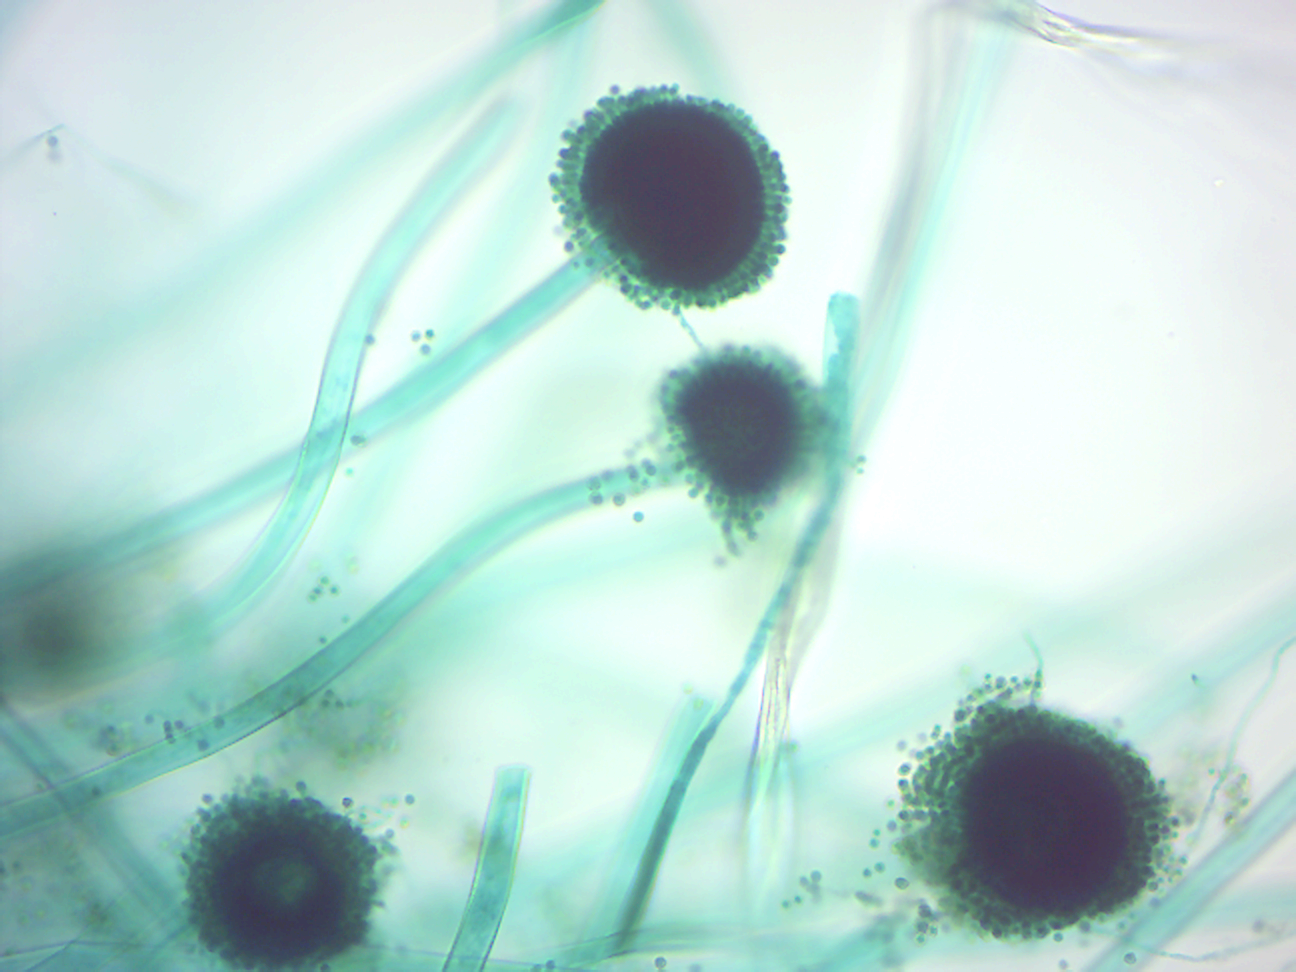
\includegraphics[width=0.7\linewidth]{./figures/fungi/aspergillus}

}

\caption{\emph{Aspergillus} conidiophores.}\label{fig:aspergillus}
\end{figure}



\begin{figure}

{\centering 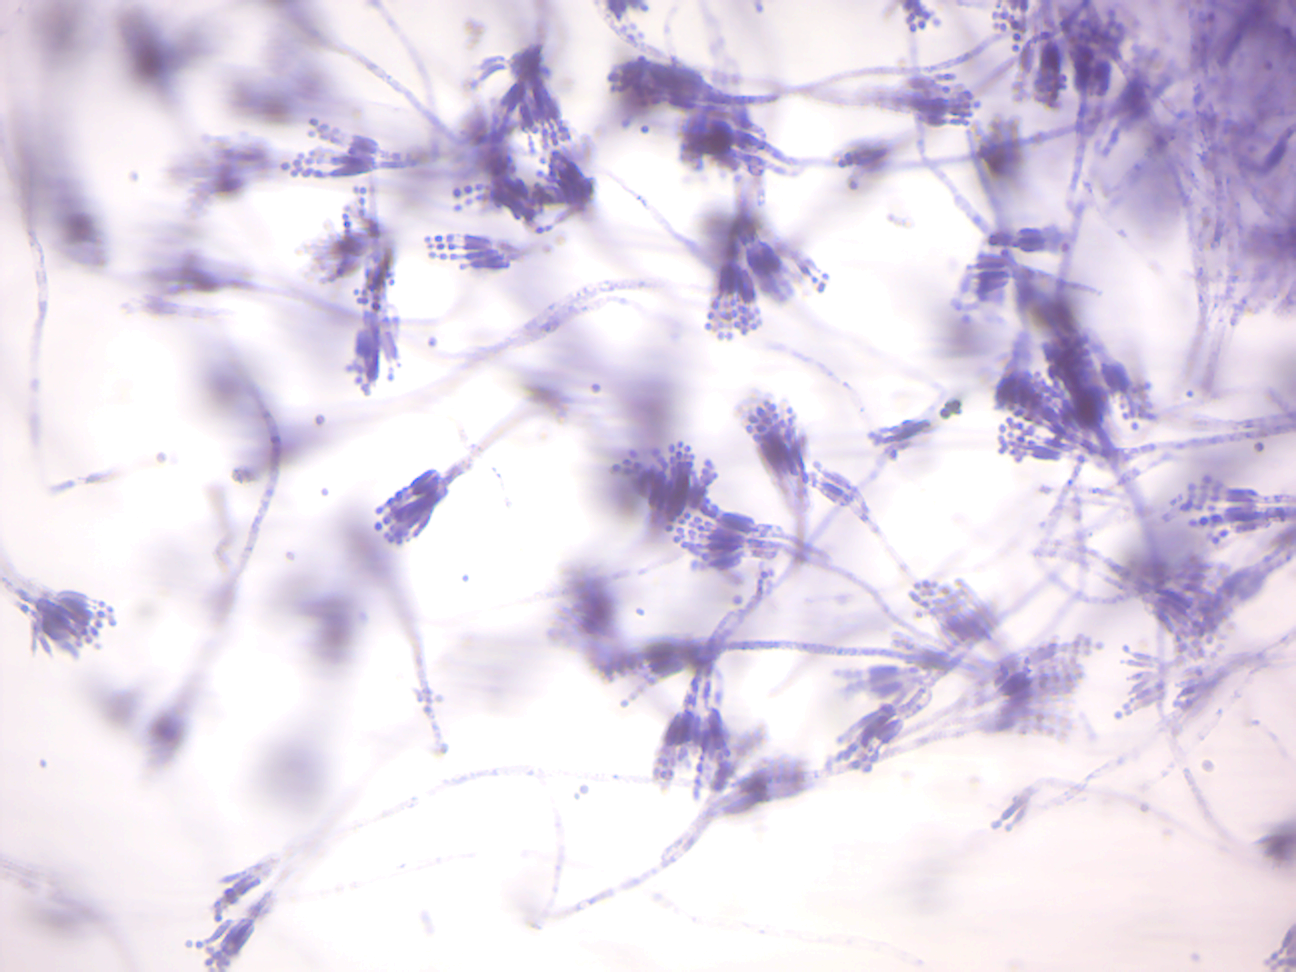
\includegraphics[width=0.7\linewidth]{./figures/fungi/penicillium}

}

\caption{\emph{Penicillium} conidiophores.}\label{fig:penicillium}
\end{figure}



\begin{figure}

{\centering 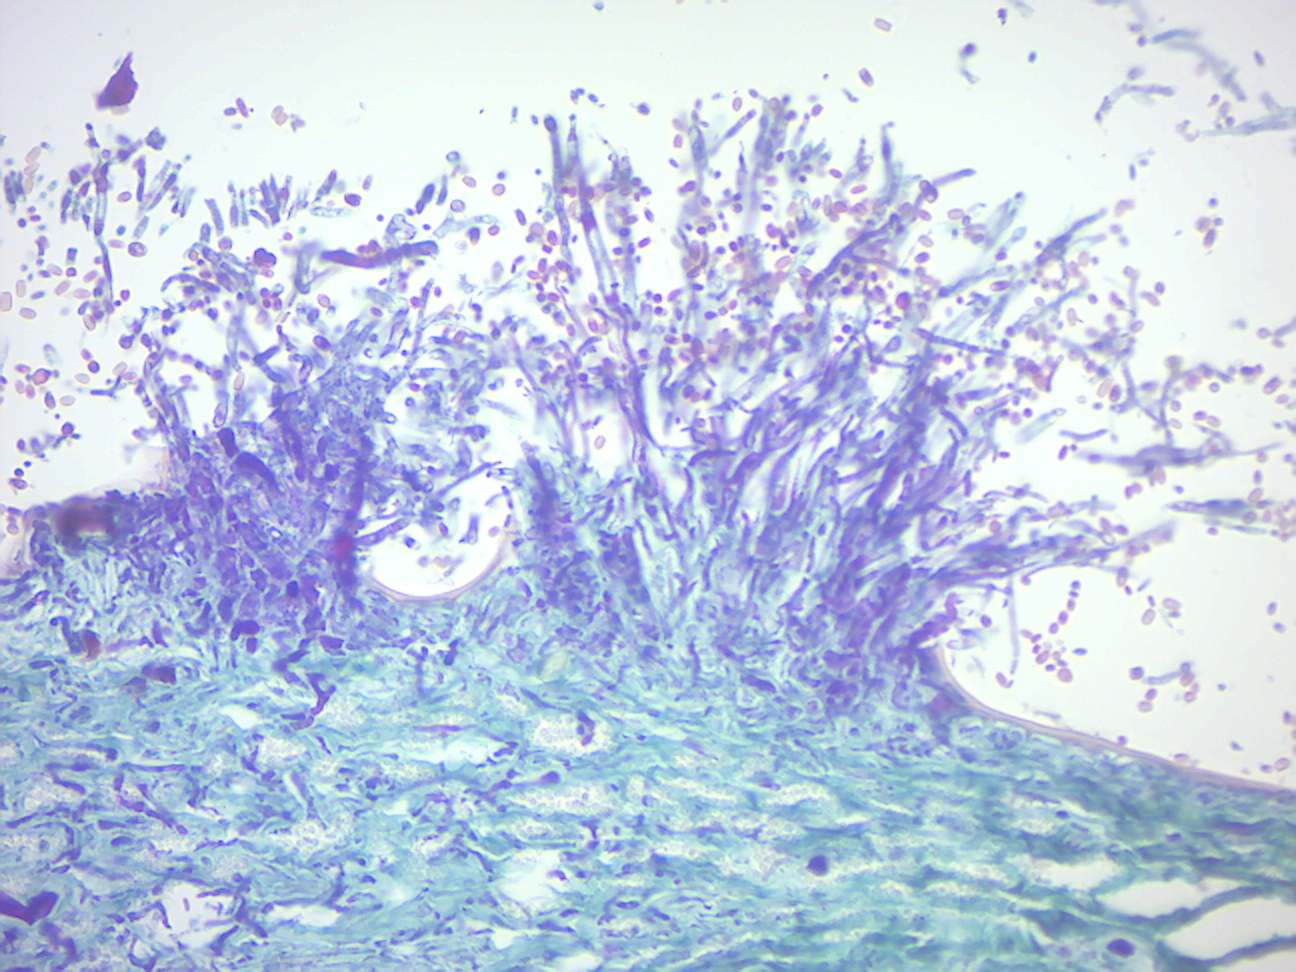
\includegraphics[width=0.7\linewidth]{./figures/fungi/penicillium_orange}

}

\caption{\emph{Penicillium} growing on orange peel.}\label{fig:orange}
\end{figure}

Sexual reproduction with meiosis has been directly observed in all
fungal phyla except Glomeromycota (genetic analysis suggests meiosis in
Glomeromycota as well). It differs in many aspects from sexual
reproduction in animals or plants. Differences also exist between fungal
groups and can be used to discriminate species by morphological
differences in sexual structures and reproductive strategies. The major
fungal groupings have initially been delineated based on the morphology
of their sexual structures and spores; for example, the spore-containing
structures, asci (sacs) and basidia (clubs), can be used in the
identification of ascomycetes (sac fungi) and basidiomycetes (club
fungi), respectively. Some species may allow mating only between
individuals of opposite mating type, whereas others can mate and
sexually reproduce with any other individual or itself. Species of the
former mating system are called heterothallic, and of the latter
homothallic.

Most fungi have both a haploid and a diploid stage in their life cycles.
In sexually reproducing fungi, compatible individuals may combine by
fusing their hyphae together into an interconnected network; this
process, anastomosis, is required for the initiation of the sexual
cycle. Many ascomycetes and basidiomycetes go through a dikaryotic
stage, in which the nuclei inherited from the two parents do not combine
immediately after cell fusion, but remain separate in the hyphal cells.

In ascomycetes, dikaryotic hyphae of the hymenium (the spore-bearing
tissue layer) form a characteristic hook at the hyphal septum. During
cell division, formation of the hook ensures proper distribution of the
newly divided nuclei into the apical and basal hyphal compartments. An
ascus (plural asci) is then formed, in which karyogamy (nuclear fusion)
occurs. Asci are embedded in an ascocarp, or fruiting body. Karyogamy in
the asci is followed immediately by meiosis and the production of
ascospores. After dispersal, the ascospores may germinate and form a new
haploid mycelium.

\section{View Prepared Slides of
Ascomycetes}\label{view-the-prepared-slides-ascomycetes}

\begin{enumerate}
\def\labelenumi{\arabic{enumi}.}
\tightlist
\item
  \href{https://en.wikipedia.org/wiki/Peziza}{\emph{Peziza}}
  (Figure \ref{fig:peziza}) apothecium

  \begin{itemize}
  \tightlist
  \item
    Locate: Hymenium layer, ascus with 8 ascospores, and infertile
    hyphae
  \end{itemize}
\item
  Yeast (Figure \ref{fig:yeast})
\end{enumerate}



\begin{figure}

{\centering 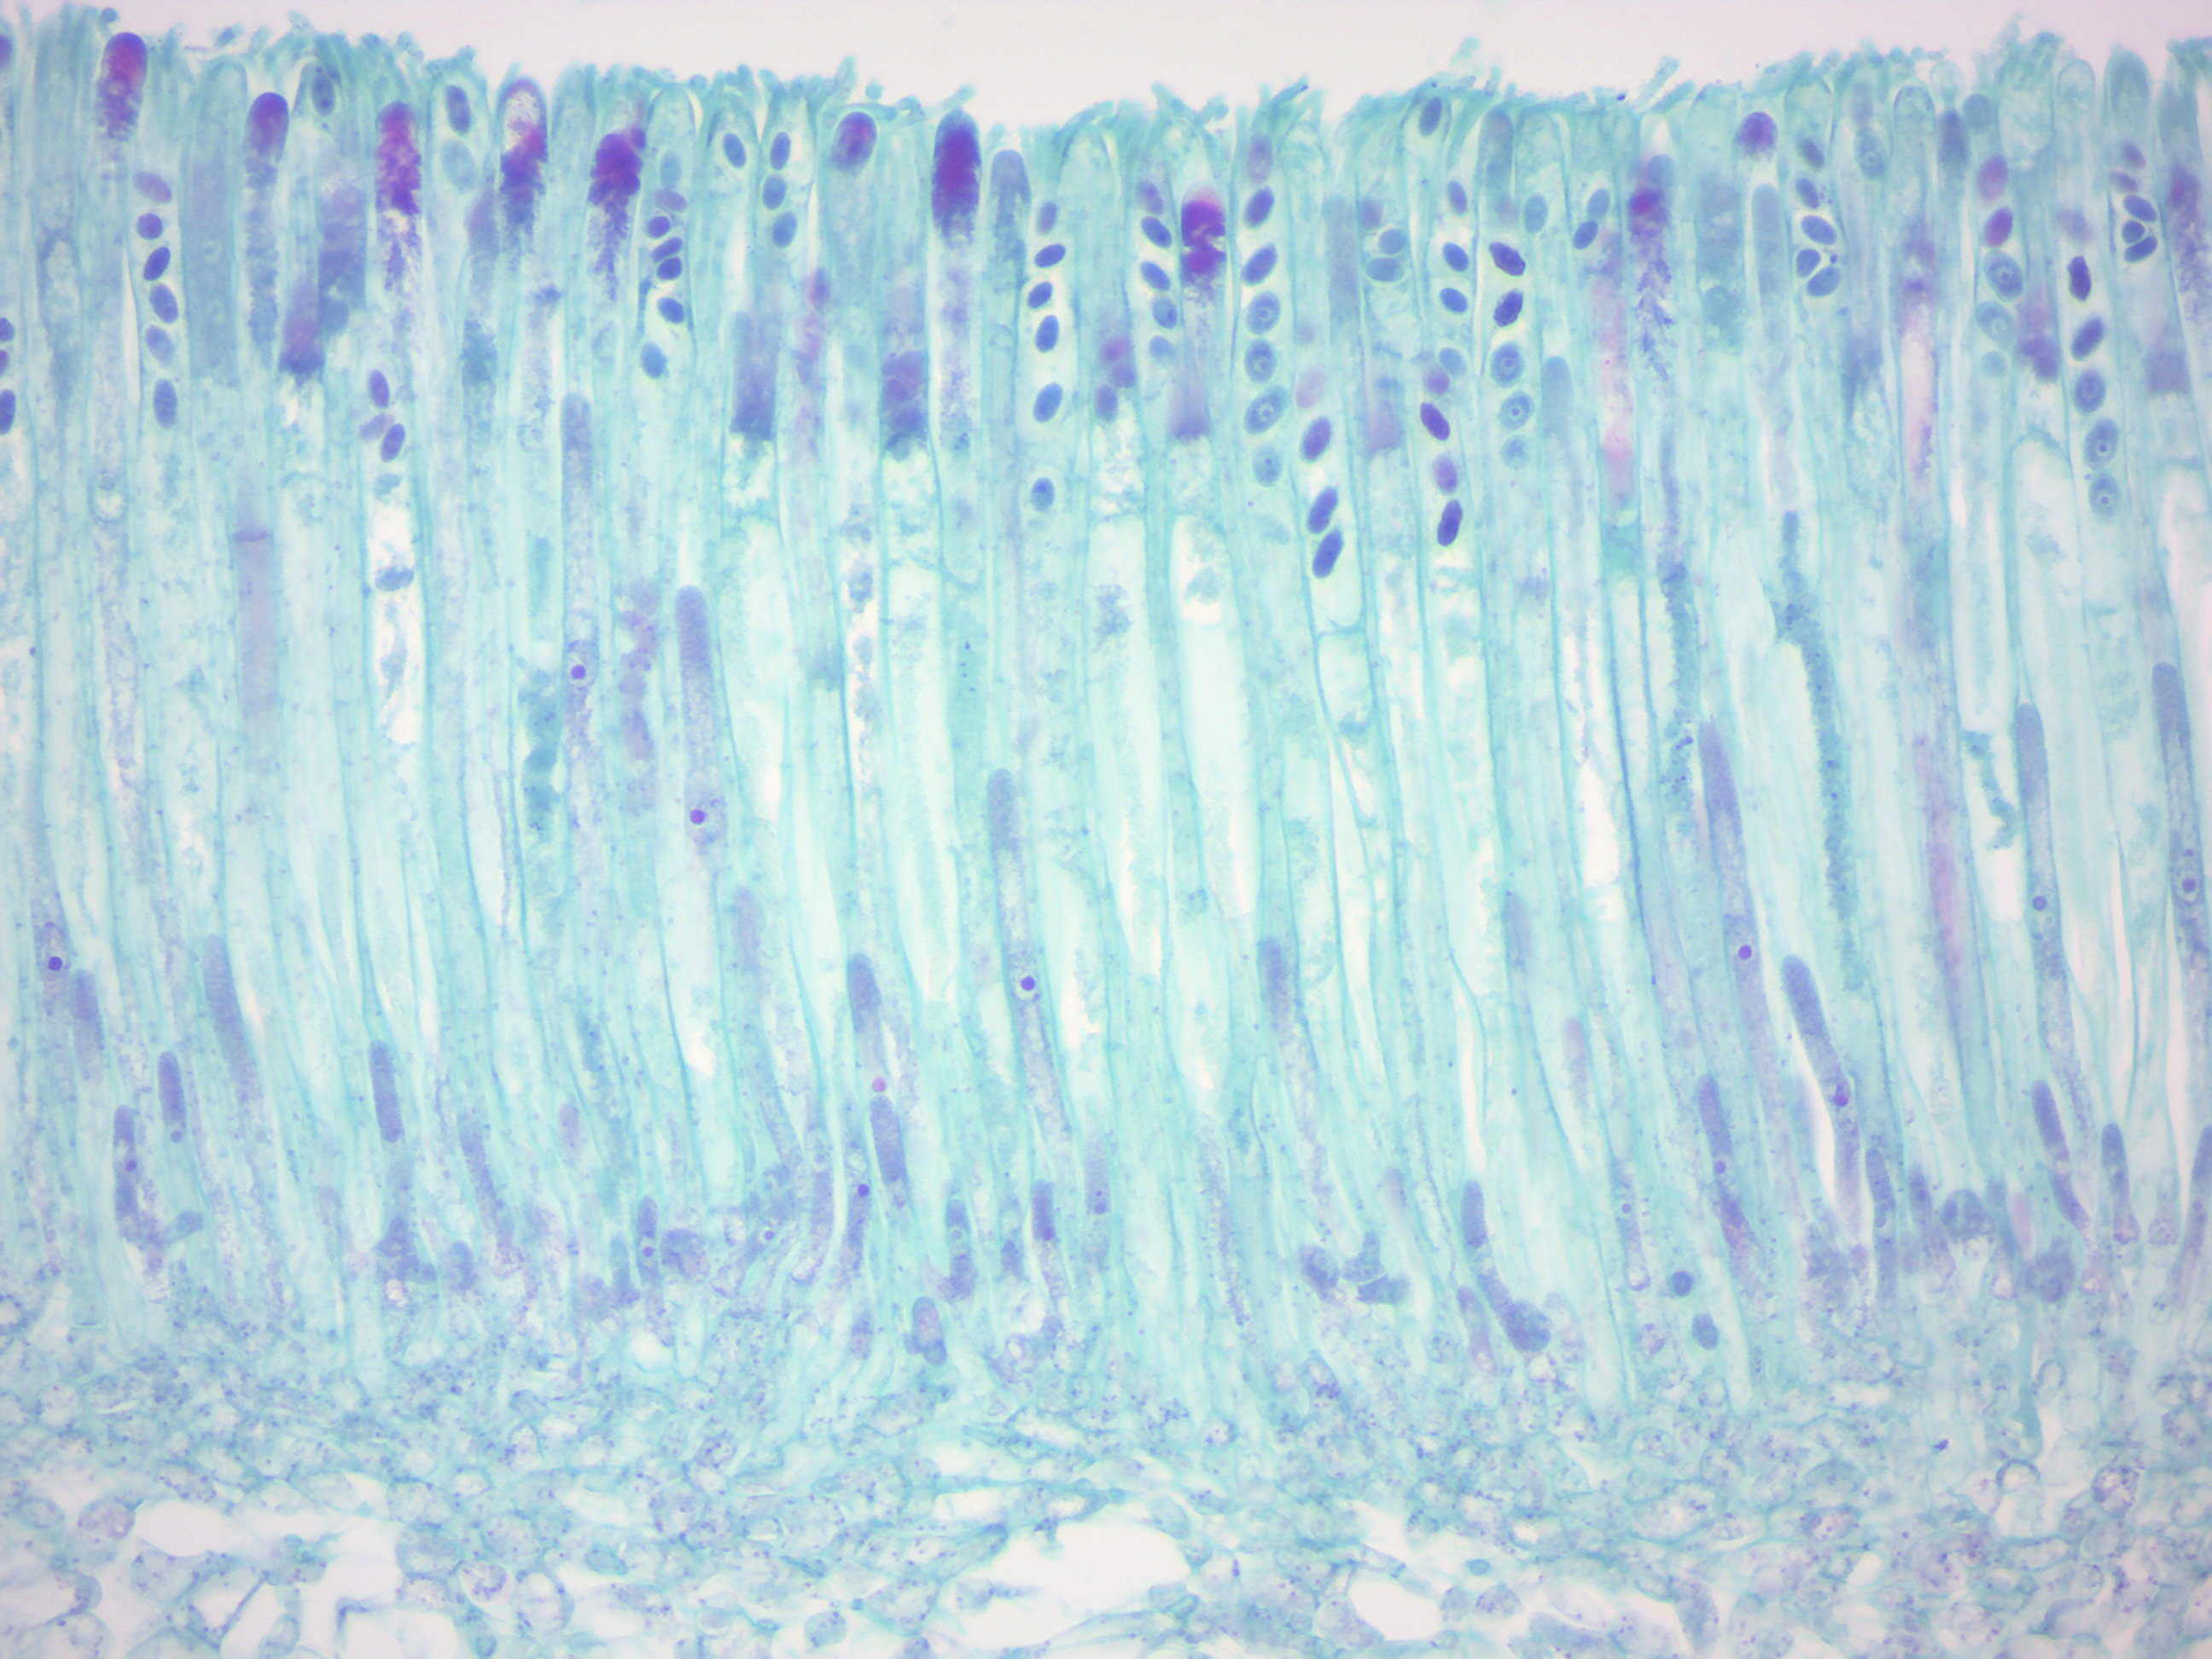
\includegraphics[width=0.7\linewidth]{./figures/fungi/peziza_apothecium}

}

\caption{\emph{Peziza} apothecium.}\label{fig:peziza}
\end{figure}

\begin{figure}

{\centering 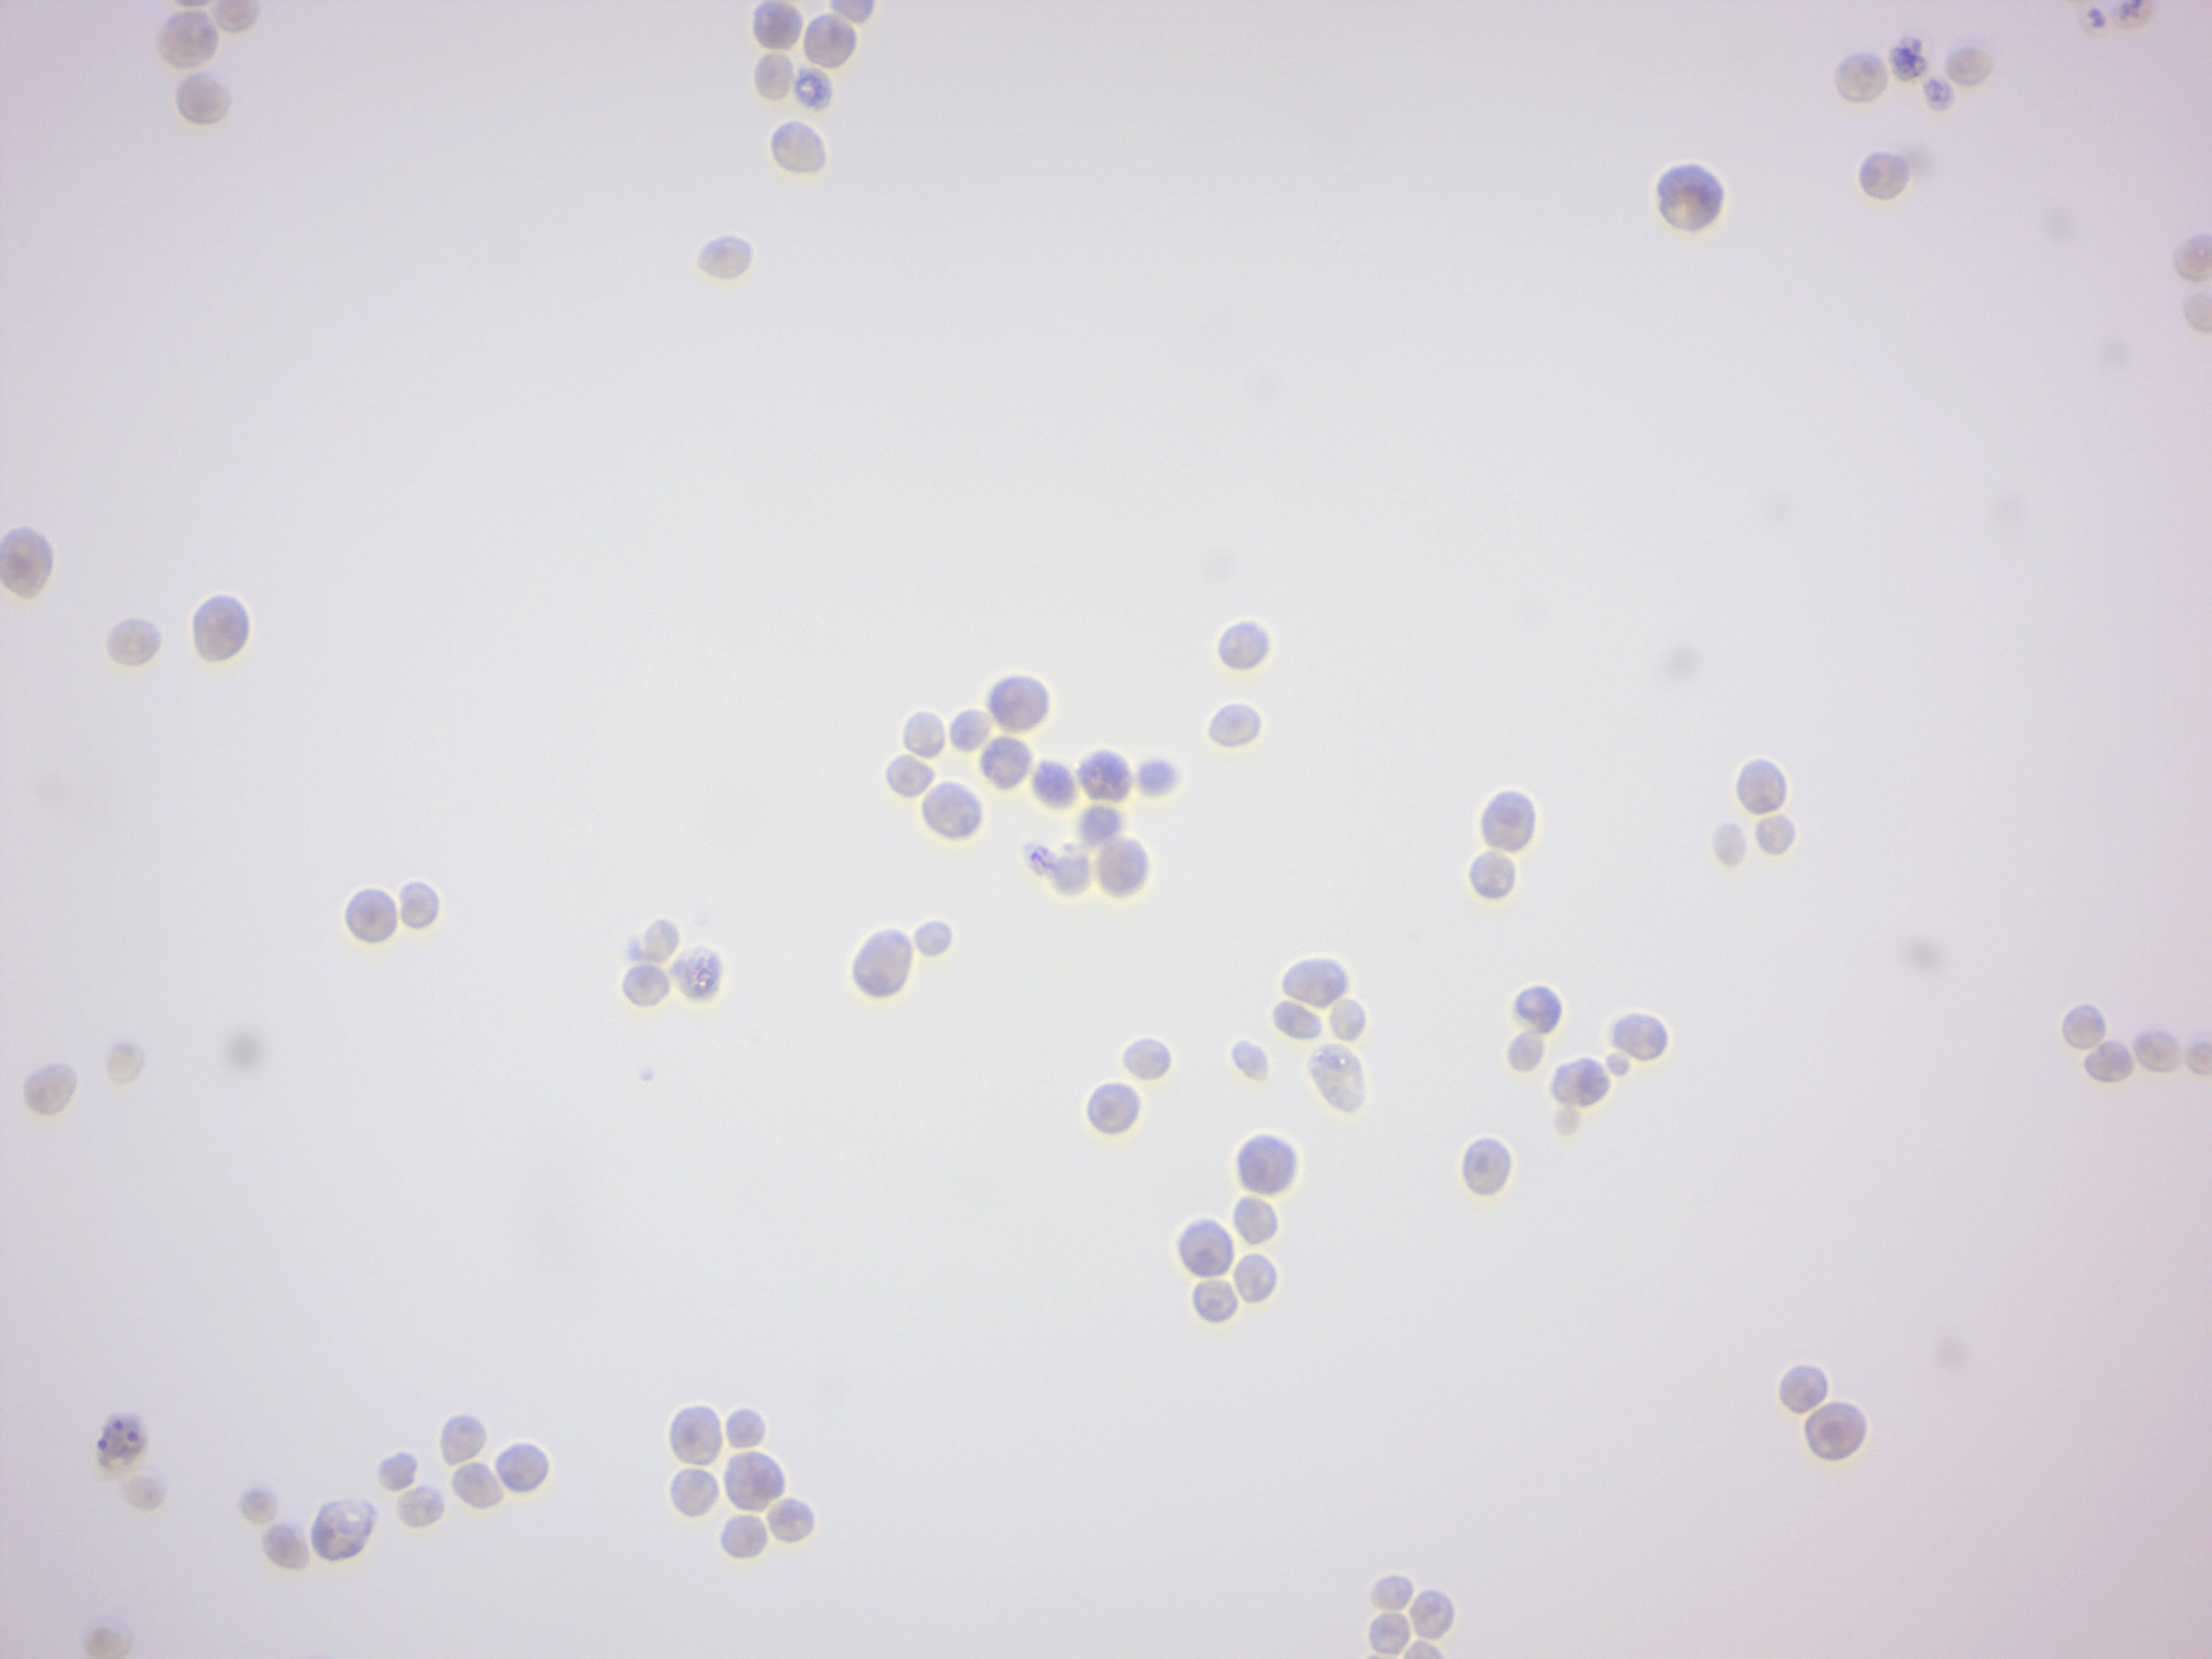
\includegraphics[width=0.7\linewidth]{./figures/fungi/yeast}

}

\caption{Yeast.}\label{fig:yeast}
\end{figure}

\section{View Prepared Slides of
Basidiomycetes}\label{view-the-prepared-slides-of-basidiomycetes}

Sexual reproduction in basidiomycetes is similar to that of the
ascomycetes. Compatible haploid hyphae fuse to produce a dikaryotic
mycelium. However, the dikaryotic phase is more extensive in the
basidiomycetes, often also present in the vegetatively growing mycelium.
A specialized anatomical structure, called a clamp connection, is formed
at each hyphal septum. As with the structurally similar hook in the
ascomycetes, the clamp connection in the basidiomycetes is required for
controlled transfer of nuclei during cell division, to maintain the
dikaryotic stage with two genetically different nuclei in each hyphal
compartment. A basidiocarp is formed in which club-like structures known
as basidia generate haploid basidiospores after karyogamy and meiosis.
The most commonly known basidiocarps are mushrooms, but they may also
take other forms.

\begin{enumerate}
\def\labelenumi{\arabic{enumi}.}
\tightlist
\item
  \href{https://en.wikipedia.org/wiki/Coprinus}{\emph{Coprinus}} (Figure
  \ref{fig:basidia})

  \begin{itemize}
  \tightlist
  \item
    Locate: gills, basidium with 4 basidiospores, hyphae
  \end{itemize}
\end{enumerate}

\begin{figure}

{\centering 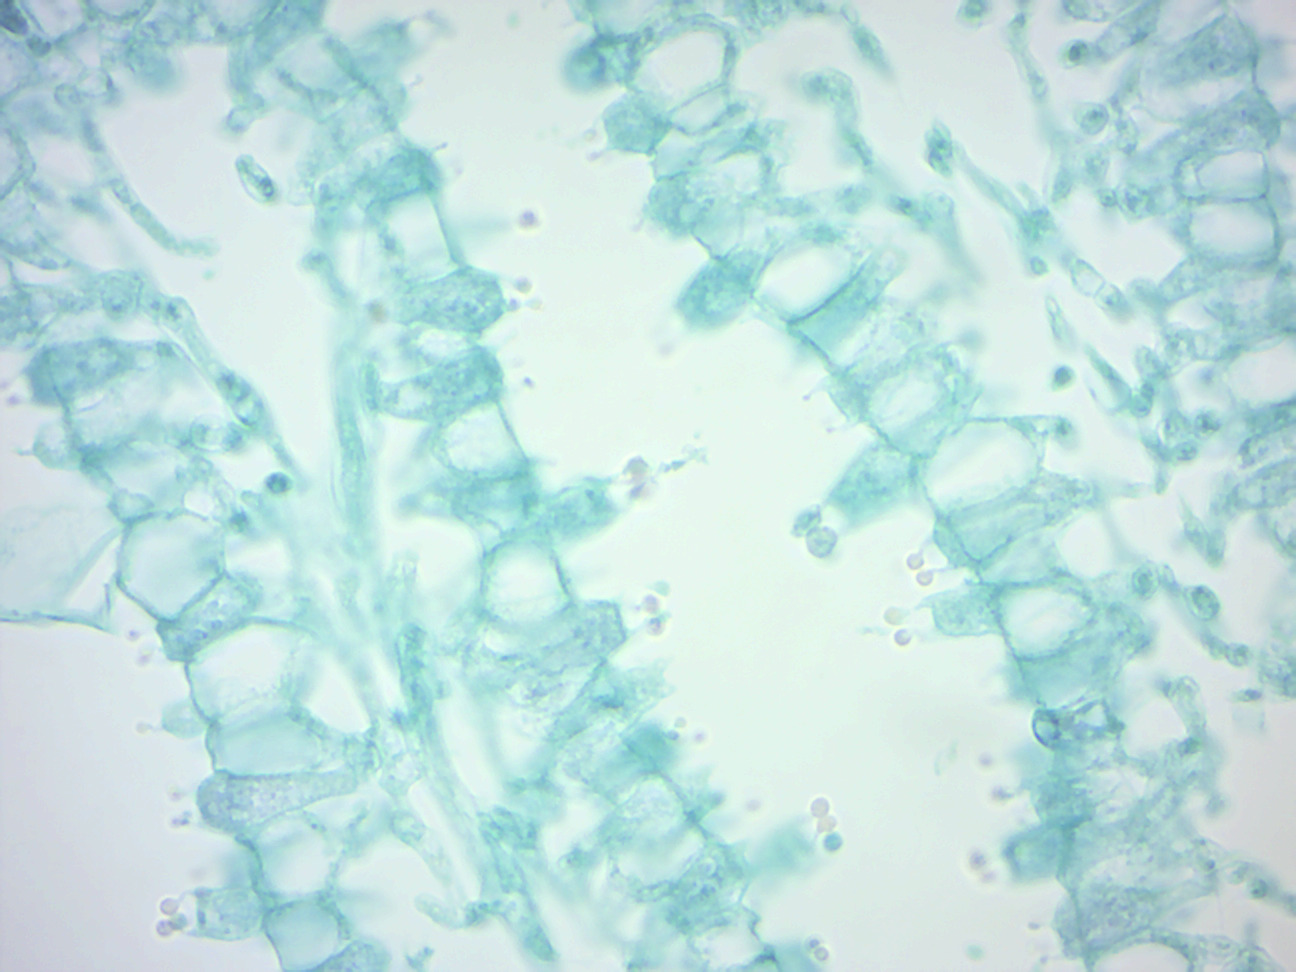
\includegraphics[width=0.7\linewidth]{./figures/fungi/basidia}

}

\caption{\emph{Coprinus} basidia with spores.}\label{fig:basidia}
\end{figure}

\section{View Prepared Slides
Glomeromycetes}\label{view-the-prepared-slides-glomeromycetes}

In glomeromycetes (formerly zygomycetes), haploid hyphae of two
individuals fuse, forming a gametangium, a specialized cell structure
that becomes a fertile gamete-producing cell. The gametangium develops
into a zygospore, a thick-walled spore formed by the union of gametes.
When the zygospore germinates, it undergoes meiosis, generating new
haploid hyphae, which may then form asexual sporangiospores. These
sporangiospores allow the fungus to rapidly disperse and germinate into
new genetically identical haploid fungal mycelia.

\begin{enumerate}
\def\labelenumi{\arabic{enumi}.}
\tightlist
\item
  \emph{Rhizopus} sporangia (Figure \ref{fig:rhizopussporangia})

  \begin{itemize}
  \tightlist
  \item
    Locate: sporangium with spores, sporangiophore, and rhizoid and
    stolon, if possible
  \end{itemize}
\item
  \emph{Rhizopus} conjugation (Figure \ref{fig:rhizopusconjugation})

  \begin{itemize}
  \tightlist
  \item
    Locate: gametangia (isogametes), zygospores, and various kinds of
    hyphae
  \end{itemize}
\item
  \emph{Rhizopus} combination (sporangia and zygotes)

  \begin{itemize}
  \tightlist
  \item
    Locate: sporangium with spores, zygospores, gametangia, and hyphae
  \end{itemize}
\end{enumerate}



\begin{figure}

{\centering 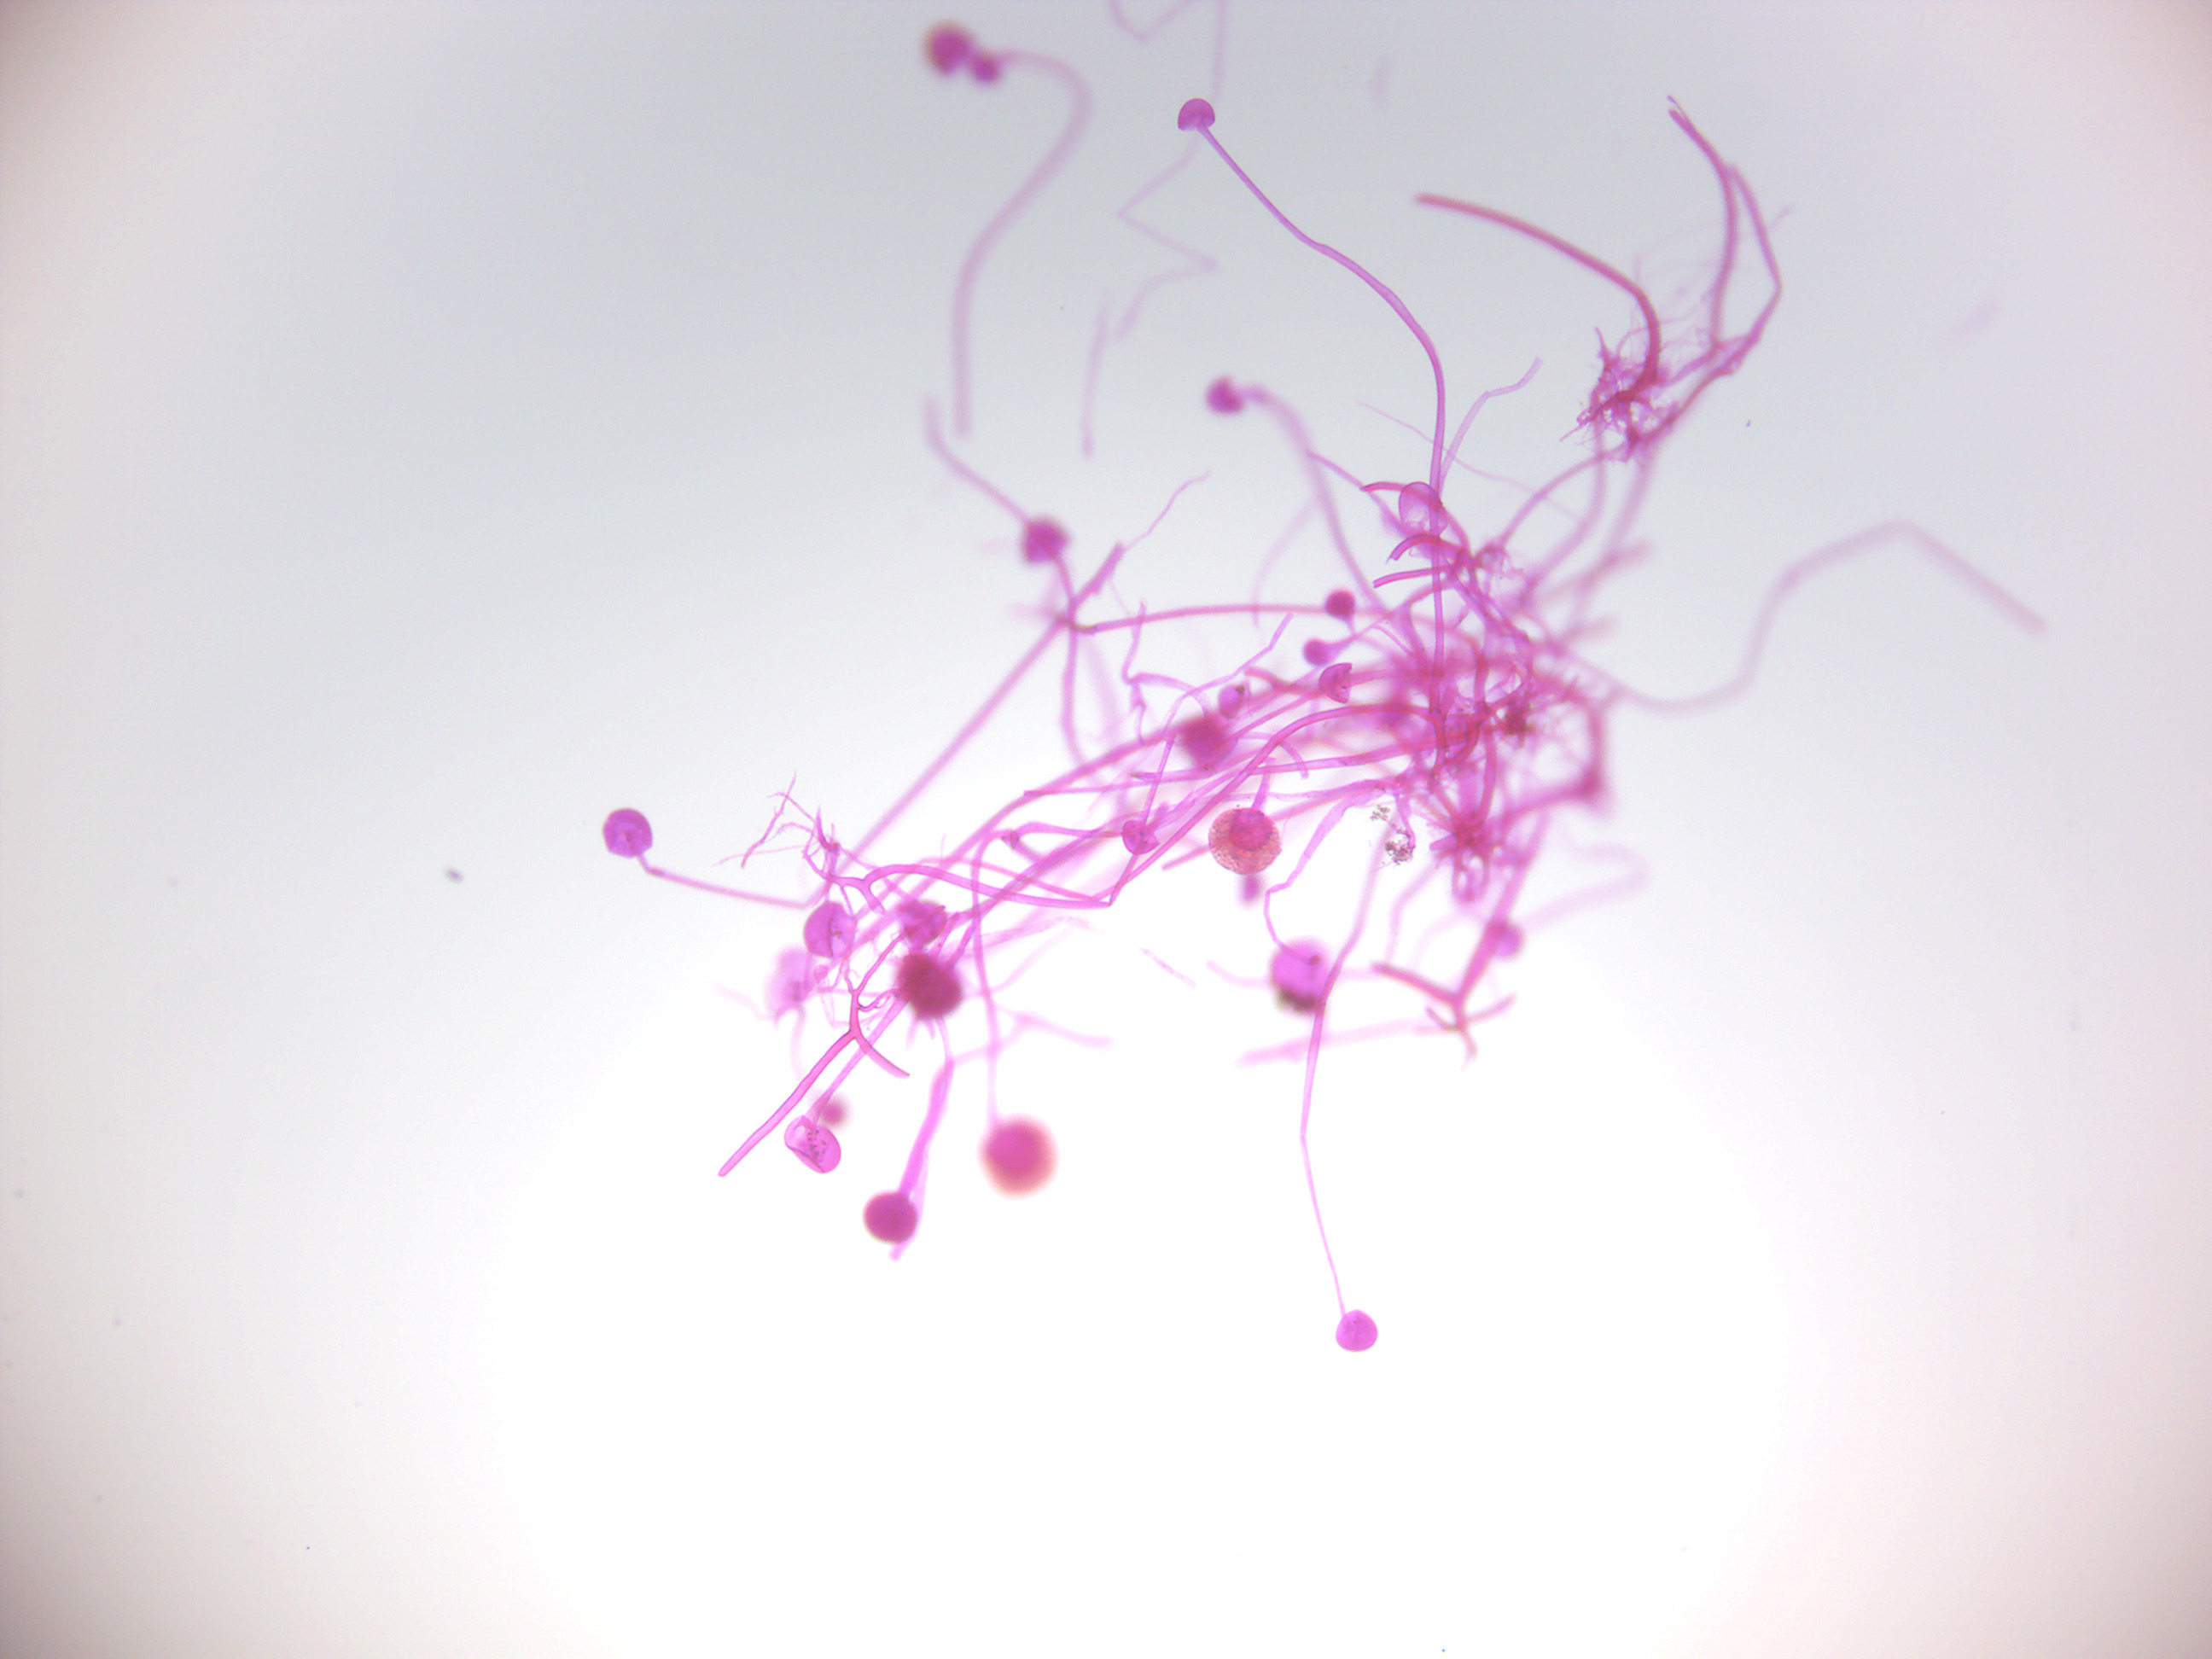
\includegraphics[width=0.7\linewidth]{./figures/fungi/rhizopus_sporangia}

}

\caption{\emph{Rhizopus} sporangia.}\label{fig:rhizopussporangia}
\end{figure}



\begin{figure}

{\centering 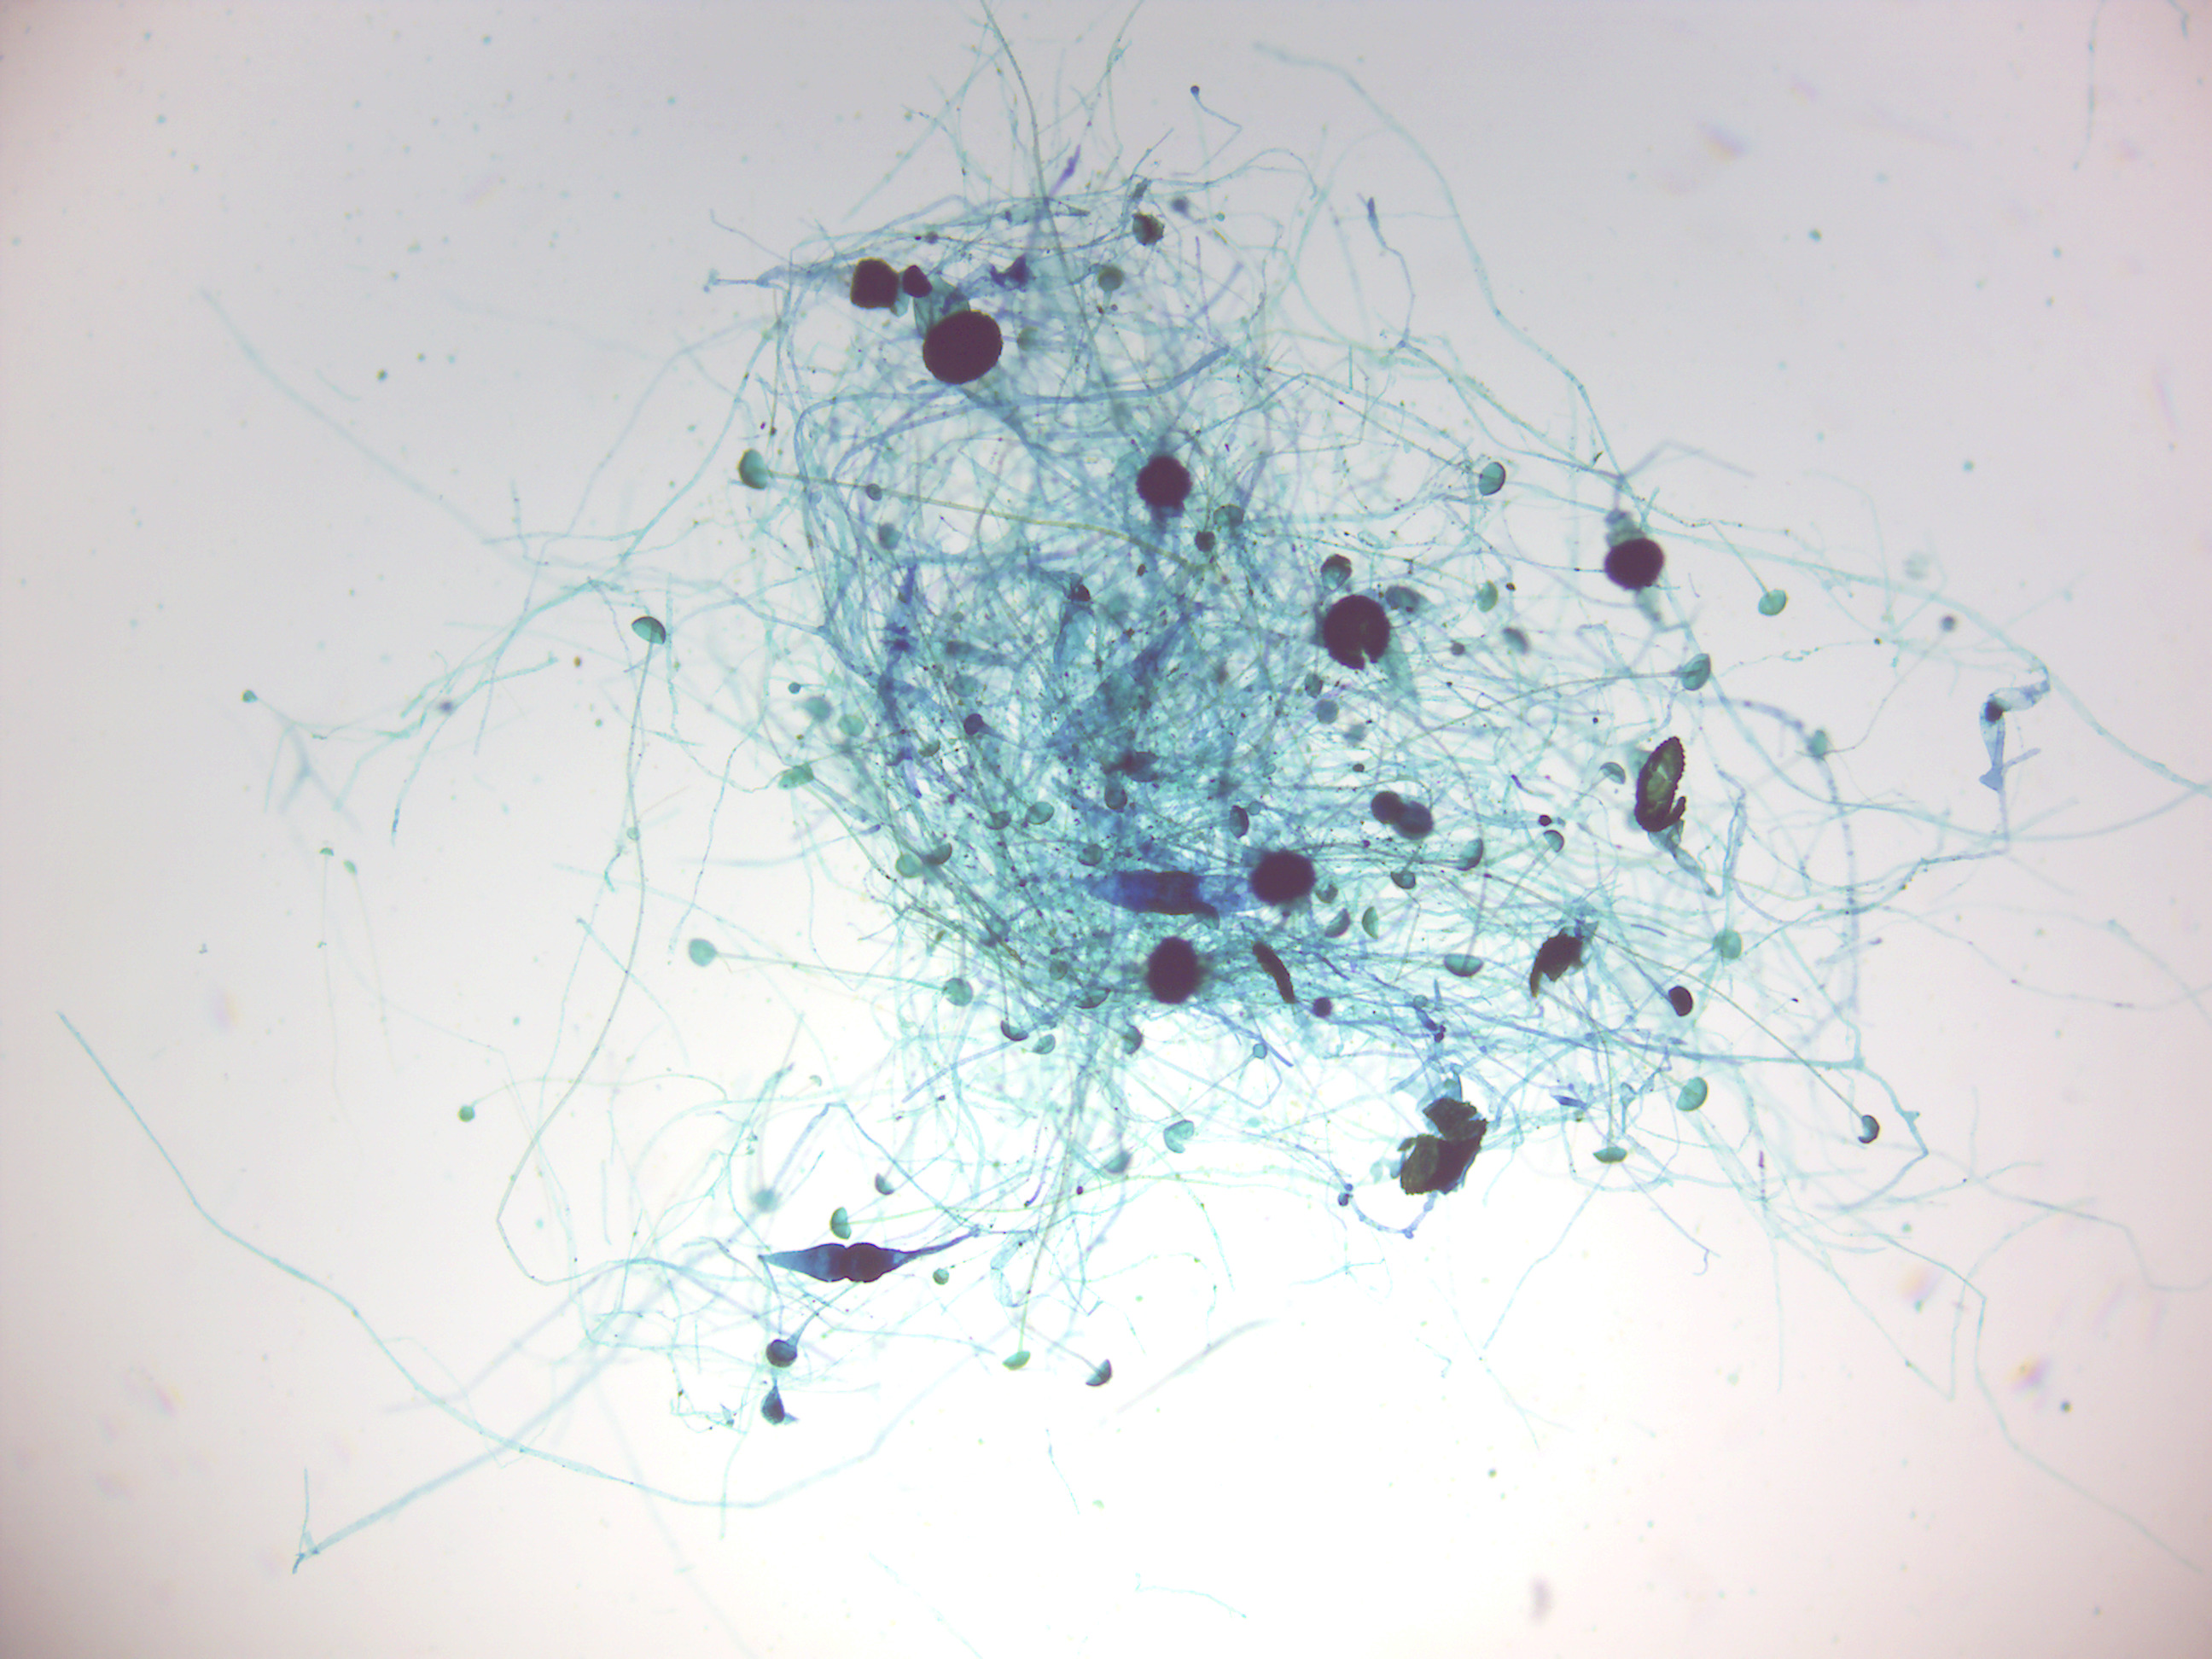
\includegraphics[width=0.7\linewidth]{./figures/fungi/rhizopus_conjugation}

}

\caption{\emph{Rhizopus} conjugation.}\label{fig:rhizopusconjugation}
\end{figure}

\section{Lichen}\label{lichen}

A \href{https://en.wikipedia.org/wiki/Lichen}{lichen} (Figure
\ref{fig:lichens}) is a composite organism that arises from algae or
cyanobacteria living among filaments of multiple fungi in a symbiotic
relationship. The combined lichen has properties different from those of
its component organisms. Lichens come in many colors, sizes, and forms.
The properties are sometimes plant-like, but lichens are not plants.
Lichens may have tiny, leafless branches (fruticose), flat leaf-like
structures (foliose), flakes that lie on the surface like peeling paint
(crustose), or other growth forms. Lichens occur from sea level to high
alpine elevations, in many environmental conditions, and can grow on
almost any surface. Lichens are abundant growing on bark, leaves,
mosses, on other lichens, and hanging from branches ``living on thin
air'' (epiphytes) in rain forests and in temperate woodland. They grow
on rock, walls, gravestones, roofs, exposed soil surfaces, and in the
soil as part of a biological soil crust. Different kinds of lichens have
adapted to survive in some of the most extreme environments on Earth:
arctic tundra, hot dry deserts, rocky coasts, and toxic slag heaps. They
can even live inside solid rock, growing between the grains. It is
estimated that 6\% of Earth's land surface is covered by lichen. There
are about 20,000 known species of lichens. Lichens may be long-lived,
with some considered to be among the oldest living things. They are
among the first living things to grow on fresh rock exposed after an
event such as a landslide. The long life-span and slow and regular
growth rate of some lichens can be used to date events.



\begin{figure}

{\centering 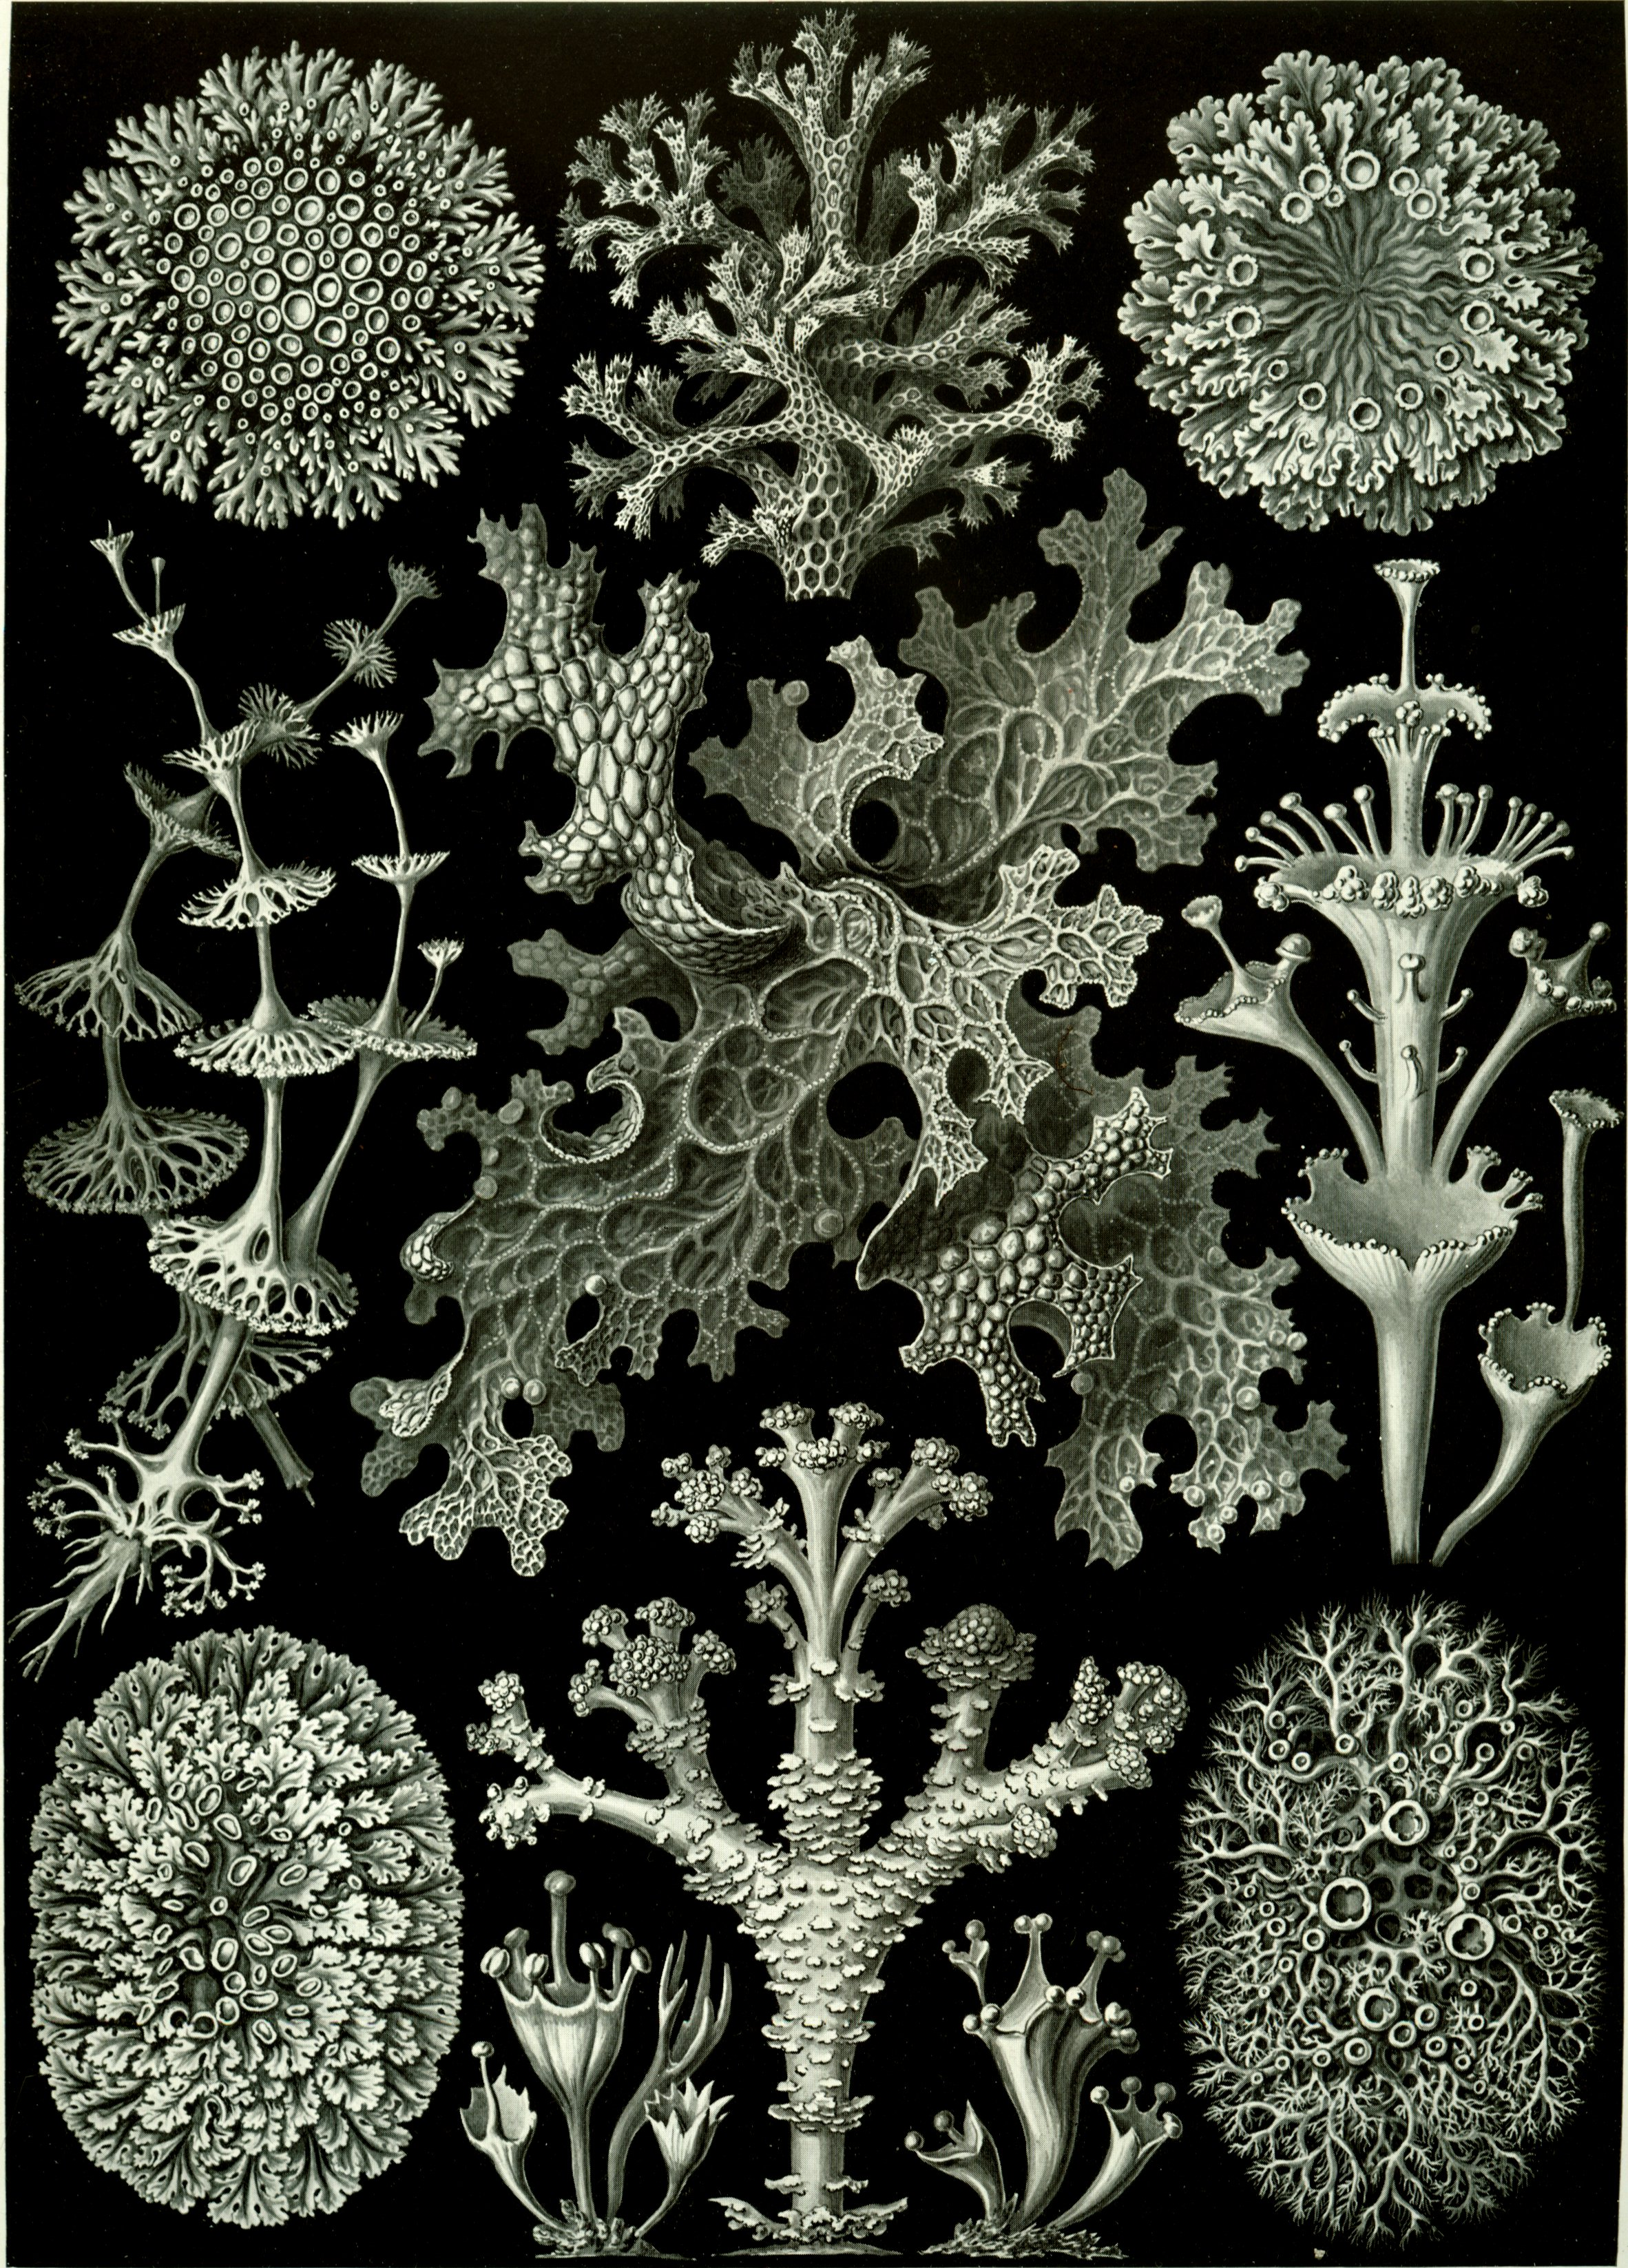
\includegraphics[width=0.7\linewidth]{./figures/fungi/Haeckel_Lichenes}

}

\caption{\href{https://commons.wikimedia.org/wiki/File:Haeckel_Lichenes.jpg}{Lichens}
from Ernst Haeckel's
\href{https://en.wikipedia.org/wiki/Kunstformen_der_Natur}{Kunstformen
der Natur}, 1904.}\label{fig:lichens}
\end{figure}

\section{View Prepared Slides of
Lichens}\label{view-the-prepared-slides-of-lichens}

\begin{enumerate}
\def\labelenumi{\arabic{enumi}.}
\tightlist
\item
  Foliose lichen thallus and apothecia (Figure \ref{fig:lichen})

  \begin{itemize}
  \tightlist
  \item
    Locate: fungal hyphae, and algal cells inside
  \end{itemize}
\end{enumerate}

\begin{figure}

{\centering 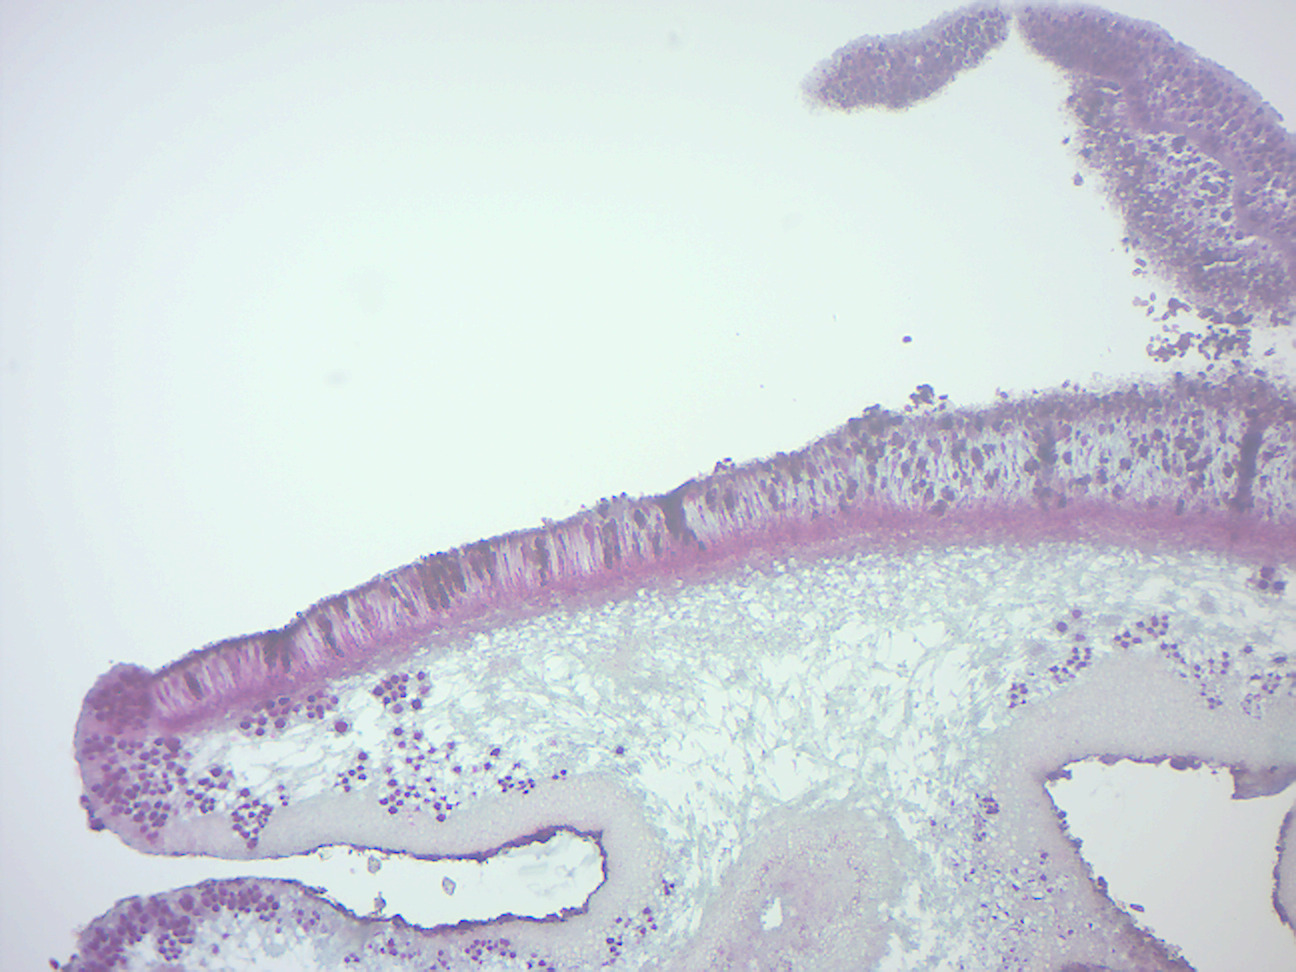
\includegraphics[width=0.7\linewidth]{./figures/fungi/foliose_lichen}

}

\caption{Foliose lichen thallus and apothecia.}\label{fig:lichen}
\end{figure}

\section{View Living Organisms}\label{view-living-organisms}

\begin{enumerate}
\def\labelenumi{\arabic{enumi}.}
\tightlist
\item
  Yeast
\item
  \emph{Rhizopus stolonifer} plate
\item
  \emph{Aspergillus} plate
\item
  \emph{Penicillium} plate
\end{enumerate}

\section{Review Questions}\label{review-questions}

\begin{enumerate}
\def\labelenumi{\arabic{enumi}.}
\tightlist
\item
  What are fungi?
\item
  How do fungi get their nutrients?
\item
  What are yeasts?
\item
  What are lichen?
\item
  What is the name of the spore containing structure in sac fungi?
\item
  In club fungi, spores are attached to
  \texttt{\_\_\_\_\_\_\_\_\_\_\_\_\_}.
\item
  What is a zygospore?
\item
  What are conidiophores?
\end{enumerate}

\chapter{Non-vascular Plants and Plants Without
Seeds}\label{non-vascular-plants-and-plants-without-seeds}

\href{https://en.wikipedia.org/wiki/Plant}{Plants} are multicellular,
photoautotrophic eukaryotes. The term Viridiplantae (Latin for ``green
plants'') includes the flowering plants, conifers and other gymnosperms,
ferns, clubmosses, hornworts, liverworts, mosses and the green algae,
and excludes the red and brown algae. Historically, plants formed one of
two kingdoms covering all living things that were not animals, and both
algae and fungi were treated as plants; however, all current definitions
of ``plant'' exclude the fungi and some algae, as well as the
prokaryotes (the archaea and bacteria).

Green plants have cell walls containing cellulose and obtain most of
their energy from sunlight via photosynthesis by primary chloroplasts,
derived from endosymbiosis with cyanobacteria. Their chloroplasts
contain chlorophylls a and b, which gives them their green color. Some
plants are parasitic and have lost the ability to produce normal amounts
of chlorophyll or to photosynthesize. Plants are characterized by sexual
reproduction and alternation of generations, although asexual
reproduction is also common.

There are over 300,000 species of plants, of which the great majority,
over 260,000, are seed plants. Green plants provide a substantial
proportion of the world's molecular oxygen and are the basis of most of
Earth's ecologies, especially on land. Plants that produce grains,
fruits and vegetables form humankind's basic foodstuffs, and have been
domesticated for millennia. Plants play many roles in culture. They are
used as ornaments and, until recently and in great variety, they have
served as the source of most medicines and drugs. The scientific study
of plants is known as botany, a branch of biology.

The evolution of plants has resulted in increasing levels of complexity,
from the earliest algal mats, through bryophytes, lycopods, ferns to the
complex gymnosperms and angiosperms of today.

\section{Embryophytes}\label{embryophytes}

The plants that are likely most familiar to us are the multicellular
land plants, called embryophytes. Embryophytes include the vascular
plants, such as ferns, conifers and flowering plants. They also include
the bryophytes, of which mosses and liverworts are the most common. All
of these plants have eukaryotic cells with cell walls composed of
cellulose, and most obtain their energy through photosynthesis, using
light, water and carbon dioxide to synthesize food. A few plant species
do not photosynthesize but are parasites on other species of
photosynthetic plants. Embryophytes are believed to have evolved from
green algae.

\section{Non-vascular plants}\label{non-vascular-plants}

Non-vascular plants are plants without a vascular system consisting of
xylem and phloem. Although non-vascular plants lack these particular
tissues, many possess simpler tissues that are specialized for internal
transport of water. Non-vascular plants do not have a wide variety of
specialized tissue types. Mosses and leafy liverworts have structures
that look like leaves but are not true leaves because they are single
sheets of cells with no stomata, no internal air spaces and have no
xylem or phloem.

\section{Bryophytes}\label{bryophytes}

\href{https://en.wikipedia.org/wiki/Bryophyte}{Bryophytes} are an
informal group consisting of three divisions of non-vascular land plants
(embryophytes), the liverworts, hornworts and mosses. They are
characteristically limited in size and prefer moist habitats although
they can survive in drier environments. The bryophytes consist of about
20,000 plant species. Bryophytes produce enclosed reproductive
structures (gametangia and sporangia), but they do not produce flowers
or seeds. They reproduce via spores. The term ``bryophyte'' comes from
bryon ``tree-moss, oyster-green'' and phyton ``plant''.

The defining features of bryophytes are:

\begin{itemize}
\tightlist
\item
  Their life cycles are dominated by the gametophyte stage.
\item
  Their sporophytes are unbranched.
\item
  They do not have a true vascular tissue containing lignin (although
  some have specialized tissues for the transport of water).
\end{itemize}

Bryophytes first appeared during the early Paleozoic. They can only
survive where moisture is available for significant periods, although
some species are desiccation-tolerant. Most species of bryophytes remain
small throughout their life-cycle. This involves an alternation between
two generations: a haploid stage, called the gametophyte, and a diploid
stage, called the sporophyte. In bryophytes, the sporophyte is always
unbranched and remains nutritionally dependent on its parent
gametophyte. The bryophytes have the ability to secrete a cuticle on
their outer surface, a waxy layer that confers resistant to desiccation.
In the mosses and hornworts, a cuticle is usually only produced on the
sporophyte. Stomata are not found in liverworts, but occur on the
sporangia of mosses and hornworts, allowing gas exchange while
controlling water loss.

\section{Mosses}\label{mosses}

\href{https://en.wikipedia.org/wiki/Moss}{Mosses}
\href{https://commons.wikimedia.org/wiki/File:Haeckel_Muscinae.jpg}{(Figure
\ref{fig:mosses})} are small flowerless plants that typically grow in
dense green clumps or mats, often in damp or shady locations. The
individual plants are usually composed of simple leaves that are
generally only one cell thick, attached to a stem that may be branched
or unbranched and has only a limited role in conducting water and
nutrients. Although some species have conducting tissues, these are
generally poorly developed and structurally different from similar
tissue found in vascular plants. Mosses do not have seeds and after
fertilization develop sporophytes with unbranched stalks topped with
single capsules containing spores. They are typically 0.2--10 cm tall,
though some species are much larger. There are approximately 12,000
species. Mosses are commonly confused with lichens, hornworts, and
liverworts.

\begin{figure}

{\centering 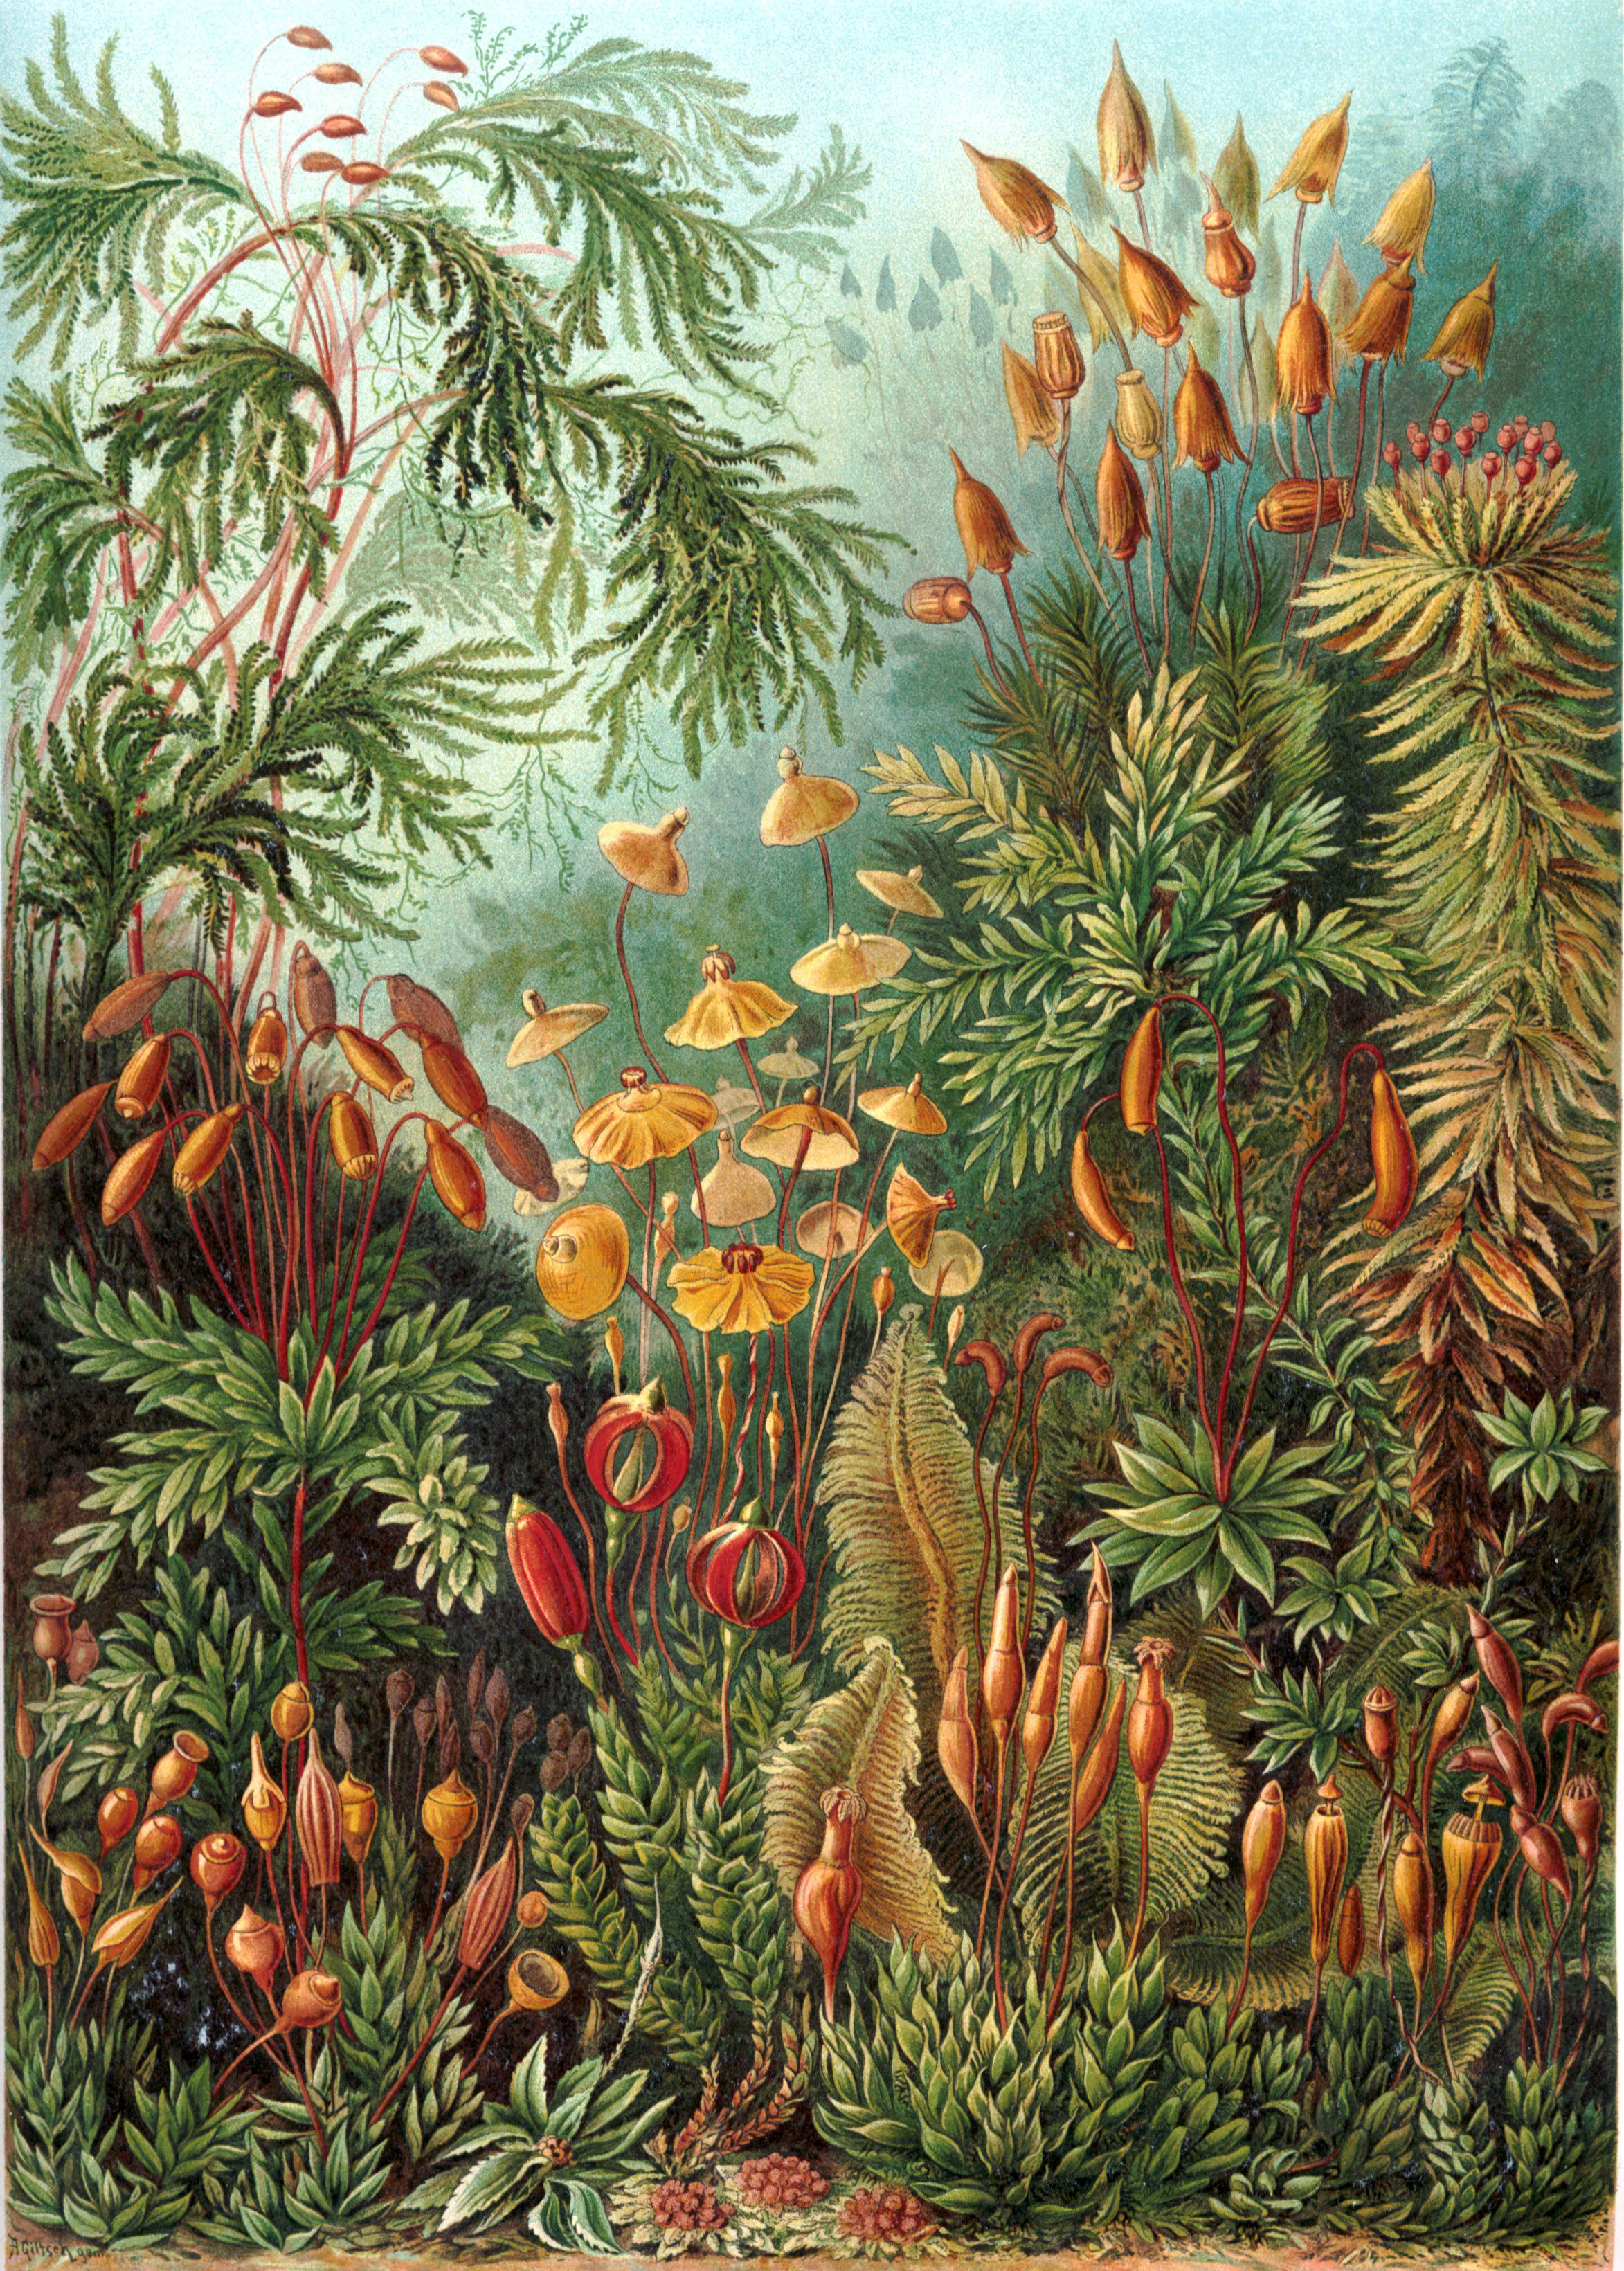
\includegraphics[width=0.7\linewidth]{./figures/mosses/Haeckel_Muscinae}

}

\caption{\href{https://commons.wikimedia.org/wiki/File:Haeckel_Muscinae.jpg}{Mosses}
from Ernst Haeckel's
\href{https://en.wikipedia.org/wiki/Kunstformen_der_Natur}{Kunstformen
der Natur}, 1904.}\label{fig:mosses}
\end{figure}

\subsection{Life cycle}\label{life-cycle}

The moss life-cycle (Figure \ref{fig:moss}) starts with a haploid spore
that germinates to produce a protonema (pl. protonemata), which is
either a mass of thread-like filaments or thalloid (flat and
thallus-like). Massed moss protonemata typically look like a thin green
felt, and may grow on damp soil, tree bark, rocks, concrete, or almost
any other reasonably stable surface. This is a transitory stage in the
life of a moss, but from the protonema grows the gametophyte that is
structurally differentiated into stems and leaves. A single mat of
protonemata may develop several gametophore shoots, resulting in a clump
of moss. From the tips of the gametophyte stems or branches develop the
sex organs of the mosses. The female organs are known as archegonia
(sing. archegonium) and are protected by a group of modified leaves
known as the perichaetum (plural, perichaeta). The archegonia are small
flask-shaped clumps of cells with an open neck (venter) down which the
male sperm swim. The male organs are known as antheridia (sing.
antheridium) and are enclosed by modified leaves called the perigonium
(pl. perigonia). The surrounding leaves in some mosses form a splash
cup, allowing the sperm contained in the cup to be splashed to
neighboring stalks by falling water droplets. In the presence of water,
sperm from the antheridia swim to the archegonia and fertilization
occurs, leading to the production of a diploid sporophyte. The sperm of
mosses is biflagellate, i.e.~they have two flagellae that aid in
propulsion. Since the sperm must swim to the archegonium, fertilization
cannot occur without water. Some species (for example \emph{Mnium hornum} or
several species of \emph{Polytrichum}) keep their antheridia in so called
`splash cups', bowl-like structures on the shoot tips that propel the
sperm several decimeters when water droplets hit it, increasing the
fertilization distance. After fertilization, the immature sporophyte
pushes its way out of the archegonial venter. It takes about a quarter
to half a year for the sporophyte to mature. The sporophyte body
comprises a long stalk, called a seta, and a capsule capped by a cap
called the operculum. The capsule and operculum are in turn sheathed by
a haploid calyptra which is the remains of the archegonial venter. The
calyptra usually falls off when the capsule is mature. Within the
capsule, spore-producing cells undergo meiosis to form haploid spores,
upon which the cycle can start again. The mouth of the capsule is
usually ringed by a set of teeth called peristome. Most mosses rely on
the wind to disperse the spores.

\begin{figure}

{\centering 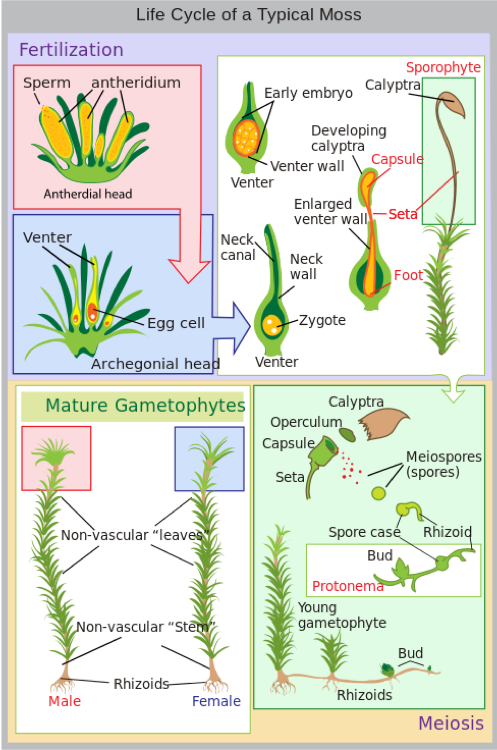
\includegraphics[width=0.7\linewidth]{./figures/mosses/moss_life_cycle}

}

\caption{\href{https://commons.wikimedia.org/wiki/File:Lifecycle_moss_svg_diagram.svg}{Life
cycle of mosses.}}\label{fig:moss}
\end{figure}

\section{View Prepared Slides of
Mosses}\label{view-the-prepared-slides-of-mosses}

\begin{enumerate}
\def\labelenumi{\arabic{enumi}.}
\tightlist
\item
  Moss archegonium (Figure \ref{fig:mossarchegonium})

  \begin{itemize}
  \tightlist
  \item
    Identify: female gametophyte tissue; archegonium with egg inside the
    venter
  \end{itemize}
\item
  Moss antheridium (Figure \ref{fig:mossantheridium})

  \begin{itemize}
  \tightlist
  \item
    Identify: male gametophyte tissue; antheridia with sperms inside;
    paraphyses (sterile filaments)
  \end{itemize}
\item
  Moss mature capsule (Figure \ref{fig:mosscapsule})

  \begin{itemize}
  \tightlist
  \item
    Identify: capsule; spores; operculum (cap); seta
  \end{itemize}
\item
  Moss protonema with bulbs w.m.

  \begin{itemize}
  \tightlist
  \item
    Identify: protonema filaments; gametophyte bulbs
  \end{itemize}
\end{enumerate}

\begin{figure}

{\centering 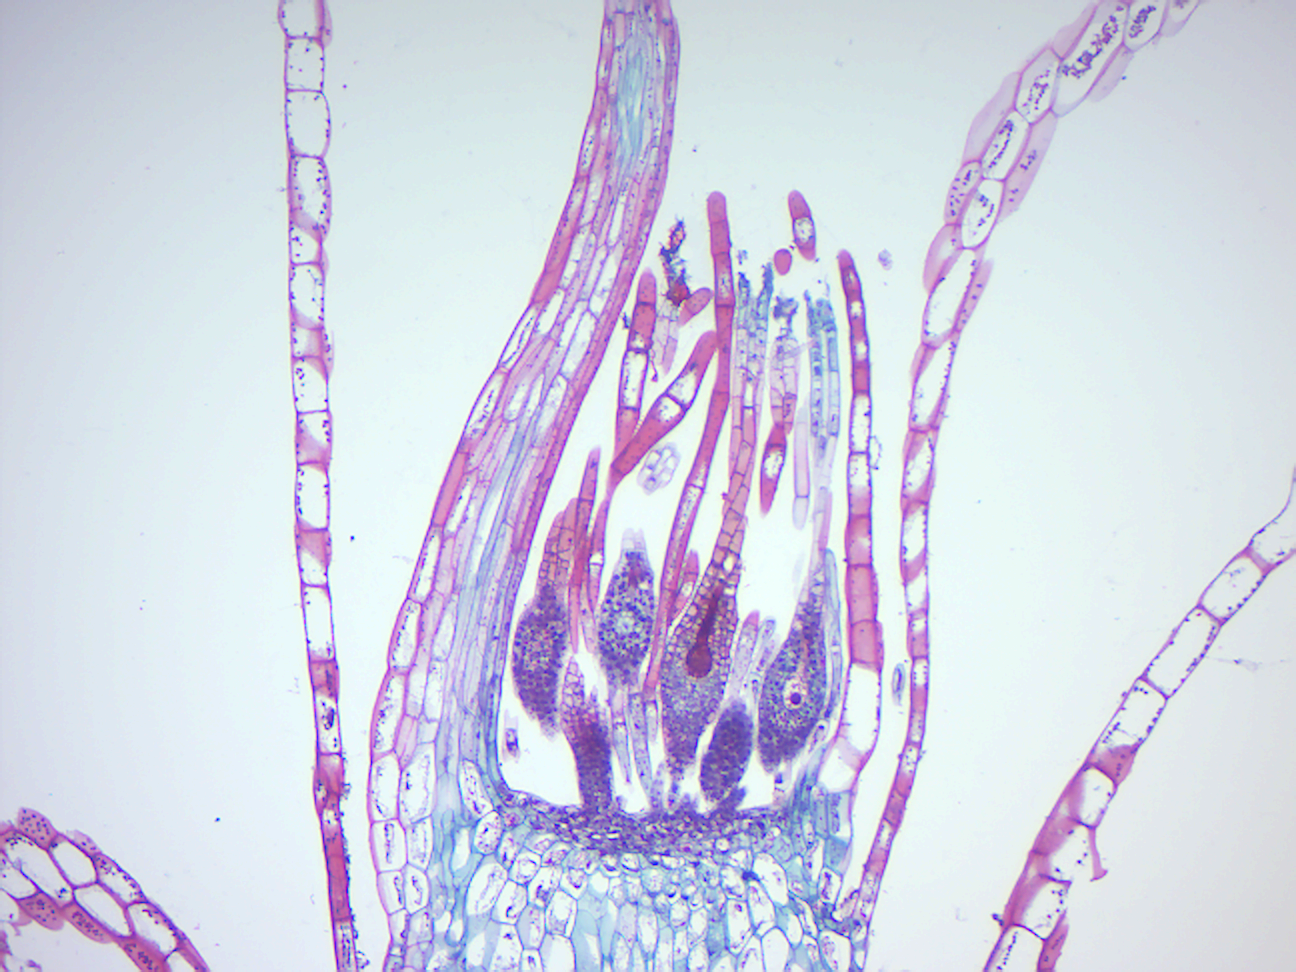
\includegraphics[width=0.7\linewidth]{./figures/mosses/moss_archegonium}

}

\caption{Moss archegonium.}\label{fig:mossarchegonium}
\end{figure}

\begin{figure}

{\centering 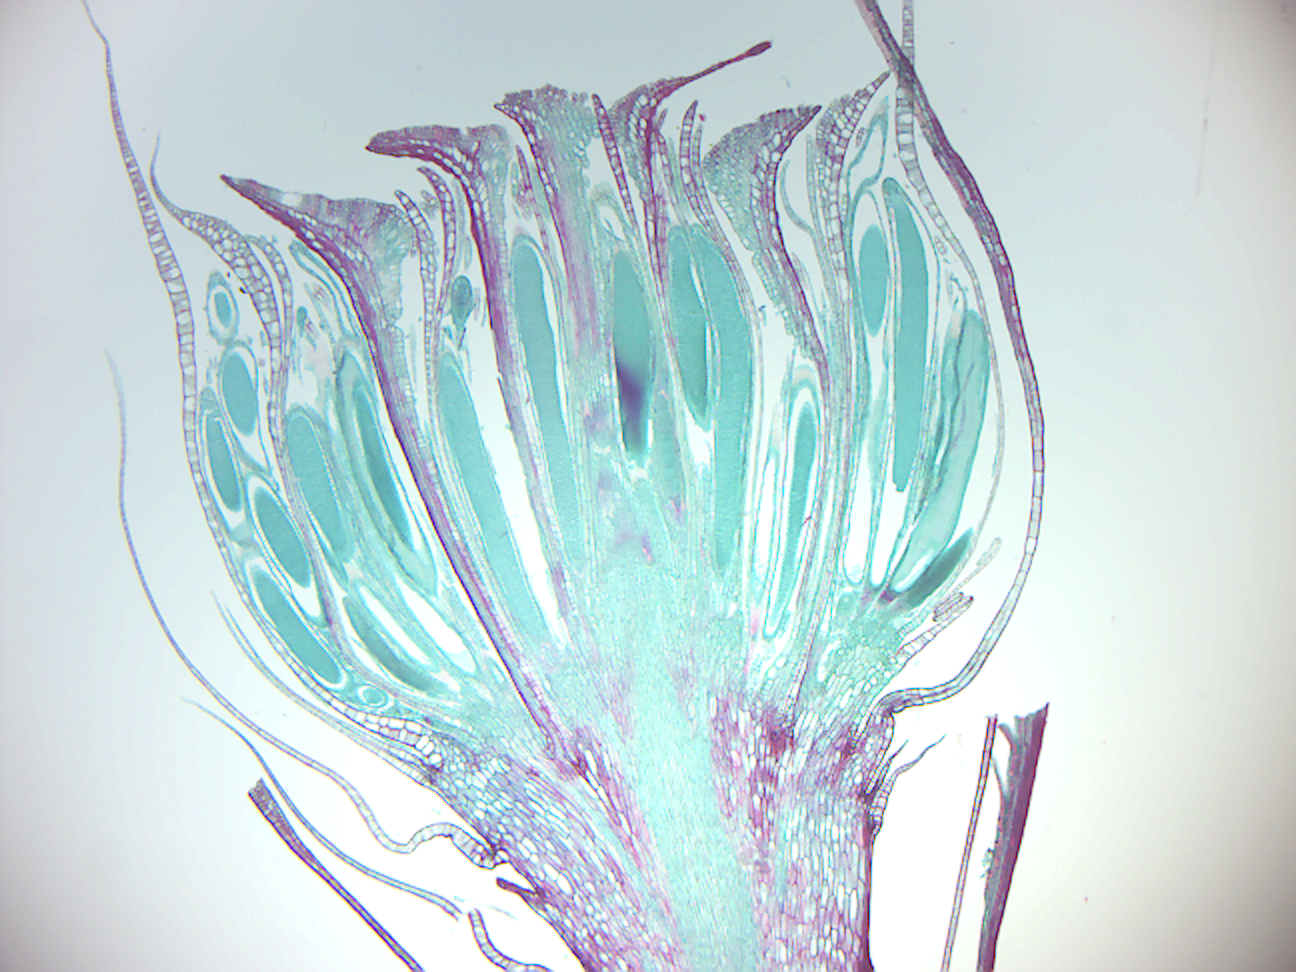
\includegraphics[width=0.7\linewidth]{./figures/mosses/moss_antheridium}

}

\caption{Moss antheridium.}\label{fig:mossantheridium}
\end{figure}

\begin{figure}

{\centering 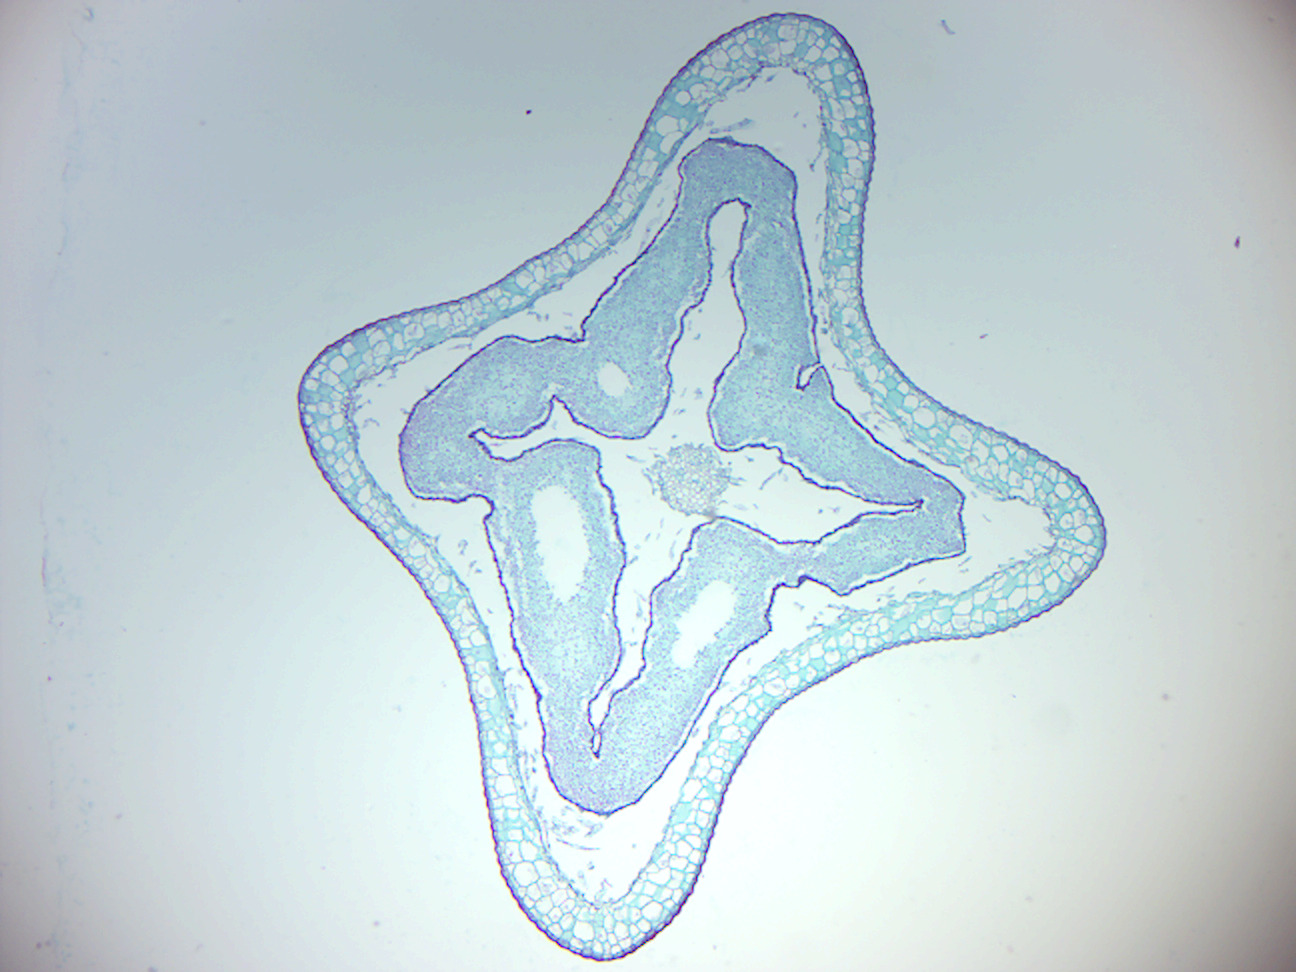
\includegraphics[width=0.7\linewidth]{./figures/mosses/moss_capsule}

}

\caption{Moss mature capsule.}\label{fig:mosscapsule}
\end{figure}

\section{Liverworts}\label{liverworts}

The
\href{https://en.wikipedia.org/wiki/Marchantiophyta}{Marchantiophyta}
(\href{https://commons.wikimedia.org/wiki/File:Haeckel_Hepaticae.jpg}{Figure
\ref{fig:hepatica}}) are a division of non-vascular land plants commonly
referred to as hepatics or liverworts. Like mosses and hornworts, they
have a gametophyte-dominant life cycle, in which cells of the plant
carry only a single set of genetic information. It is estimated that
there are about 9000 species of liverworts. Some of the more familiar
species grow as a flattened leafless thallus, but most species are leafy
with a form very much like a flattened moss. Liverworts are typically
small, usually from 2--20 mm wide with individual plants less than 10 cm
long, and are therefore often overlooked. However, certain species may
cover large patches of ground, rocks, trees or any other reasonably firm
substrate on which they occur. They are distributed globally in almost
every available habitat, most often in humid locations although there
are desert and Arctic species as well. Some species can be a nuisance in
shady greenhouses or a weed in gardens.

\begin{figure}

{\centering 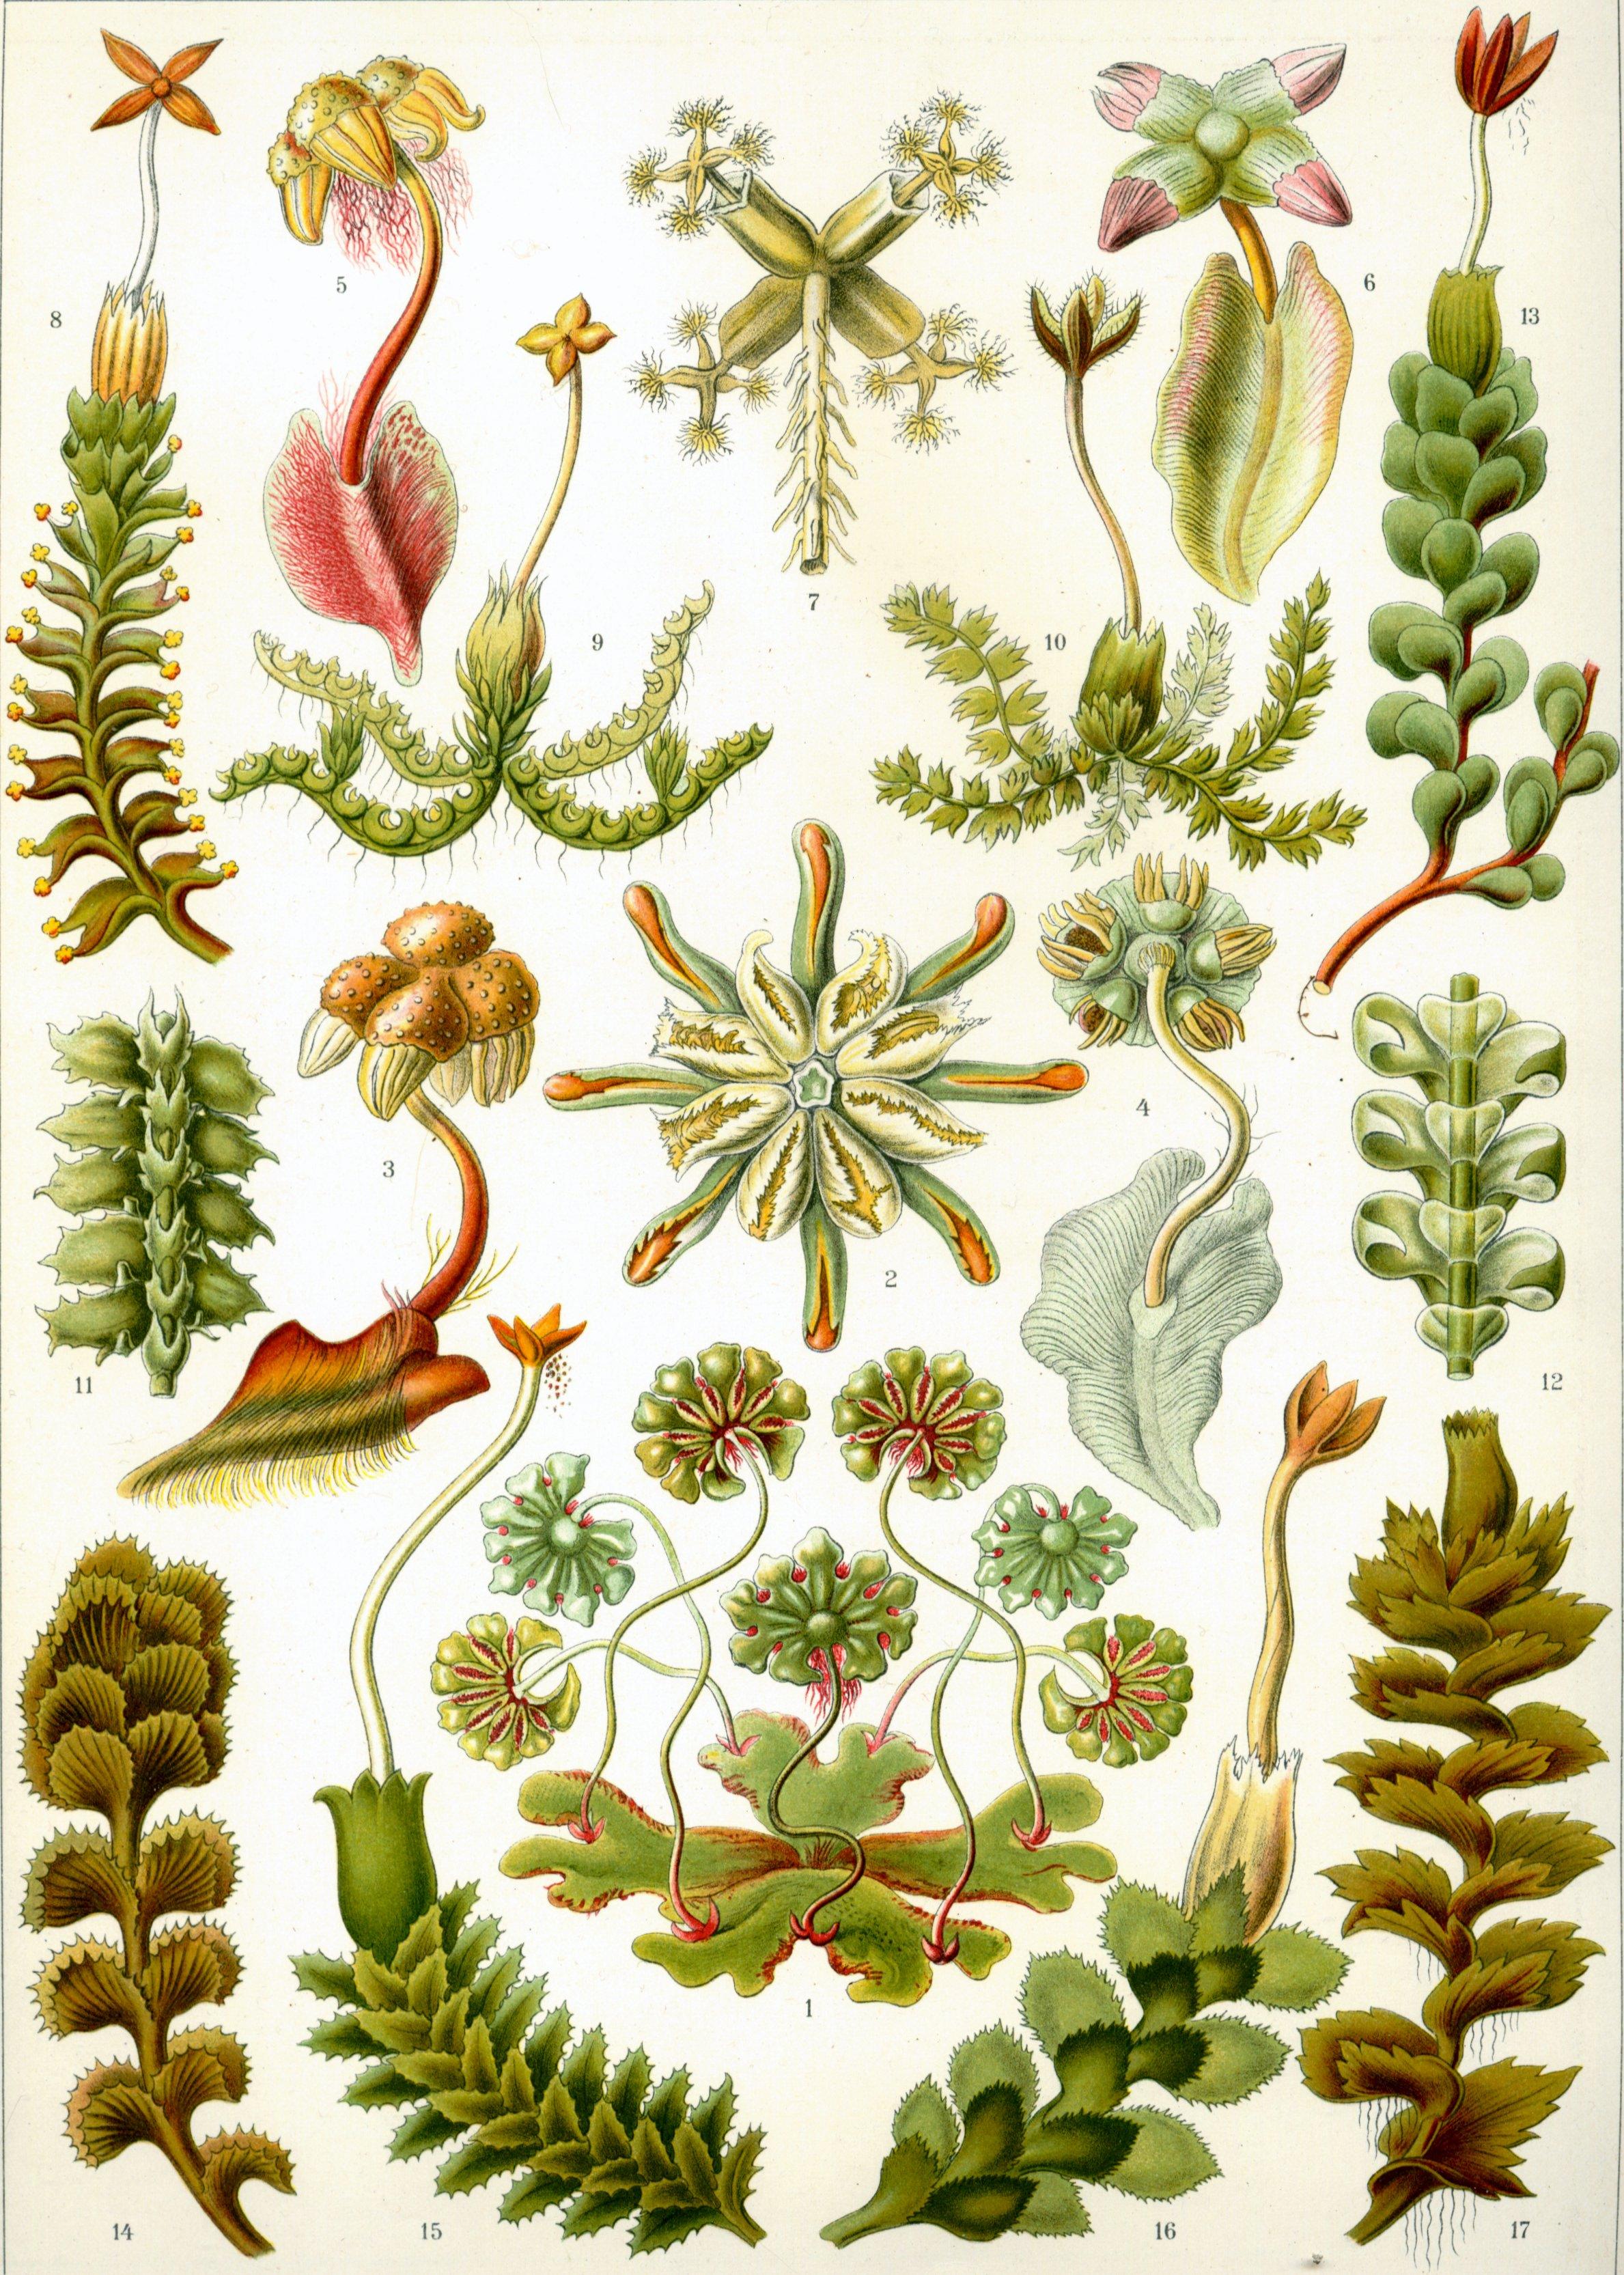
\includegraphics[width=0.7\linewidth]{./figures/mosses/Haeckel_Hepaticae}

}

\caption{\href{https://commons.wikimedia.org/wiki/File:Haeckel_Hepaticae.jpg}{Liverworts}
from Ernst Haeckel's
\href{https://en.wikipedia.org/wiki/Kunstformen_der_Natur}{Kunstformen
der Natur}, 1904.}\label{fig:hepatica}
\end{figure}

\subsection{Life cycle}\label{life-cycle-1}

The life of a liverwort starts from the germination of a haploid spore
to produce a protonema, which is either a mass of thread-like filaments
or else a flattened thallus. The protonema is a transitory stage in the
life of a liverwort, from which will grow the mature gametophyte plant
that produces the sex organs. The male organs are known as antheridia
(singular: antheridium) and produce the sperm cells. Clusters of
antheridia are enclosed by a protective layer of cells called the
perigonium (plural: perigonia). As in other land plants, the female
organs are known as archegonia (singular: archegonium) and are protected
by the thin surrounding perichaetum (plural: perichaeta). Each
archegonium has a slender hollow tube, the ``neck'', down which the
sperm swim to reach the egg cell. Liverwort species may be either
dioecious or monoecious. In dioecious liverworts, female and male sex
organs are borne on different and separate gametophyte plants. In
monoecious liverworts, the two kinds of reproductive structures are borne
on different branches of the same plant. In either case, the sperm must
move from the antheridia where they are produced to the archegonium
where the eggs are held. The sperm of liverworts is biflagellate,
i.e.~they have two tail-like flagellae that enable them to swim short
distances, provided that at least a thin film of water is present. Their
journey may be assisted by the splashing of raindrops. When sperm reach
the archegonia, fertilization occurs, leading to the production of a
diploid sporophyte. After fertilization, the immature sporophyte within
the archegonium develops three distinct regions: (1) a foot, which both
anchors the sporophyte in place and receives nutrients from its
``mother'' plant, (2) a spherical or ellipsoidal capsule, inside which
the spores will be produced for dispersing to new locations, and (3) a
seta (stalk) which lies between the other two regions and connects them.
When the sporophyte has developed all three regions, the seta elongates,
pushing its way out of the archegonium and rupturing it. While the foot
remains anchored within the parent plant, the capsule is forced out by
the seta and is extended away from the plant and into the air. Within
the capsule, cells divide to produce both elater cells and
spore-producing cells. The elaters are spring-like, and will push open
the wall of the capsule to scatter themselves when the capsule bursts.
The spore-producing cells will undergo meiosis to form haploid spores to
disperse, upon which point the life cycle can start again. Some
liverworts are capable of asexual reproduction. Some thallose liverworts
such as \emph{Marchantia polymorpha} produce small disc-shaped gemmae in
shallow cups. \emph{Marchantia} gemmae can be dispersed up to 120 cm by rain
splashing into the cups.

\begin{figure}

{\centering 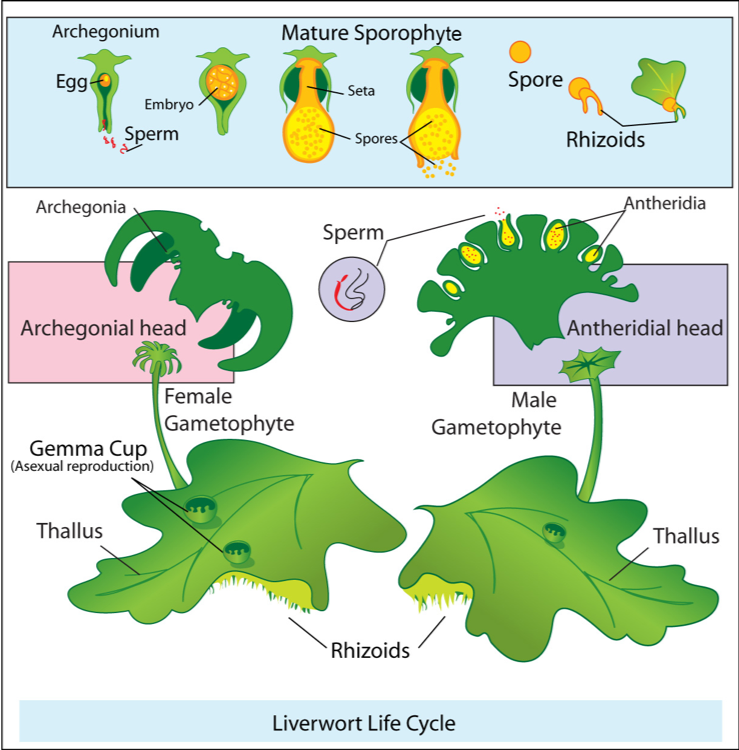
\includegraphics[width=0.7\linewidth]{./figures/mosses/liverwort_life_cycle}

}

\caption{\href{https://commons.wikimedia.org/wiki/File:Liverwort_life_cycle.jpg}{Life
cycle of liverworts.}
}\label{fig:liverwort}
\end{figure}

\section{View Prepared Slides of
Liverworts}\label{view-prepared-slides-of-liverworts}

\begin{enumerate}
\def\labelenumi{\arabic{enumi}.}
\tightlist
\item
  \emph{Marchantia} life history
\item
  \emph{Marchantia} thallus (Figure \ref{fig:marchantiathallus})

  \begin{itemize}
  \tightlist
  \item
    Identify: pores, tissue of lamina, rhizoids
  \end{itemize}
\item
  \emph{Marchantia} archegonia

  \begin{itemize}
  \tightlist
  \item
    Identify: archegonium with egg inside the venter; tissue of
    archegoniophore (female gametophyte)
  \end{itemize}
\item
  \emph{Marchantia} antheridia (Figure \ref{fig:marchantiaantheridia})

  \begin{itemize}
  \tightlist
  \item
    Identify: antheridia with sperms; tissue of antheridiophore (Male
    gametophyte); air chambers
  \end{itemize}
\item
  \emph{Marchantia} sporophyte (Figure \ref{fig:marchantiasporophyte})

  \begin{itemize}
  \tightlist
  \item
    Identify: sporophyte and its three parts: foot, seta (stalk), and
    capsule; spores and elaters inside the capsule; tissue of the female
    gametophyte
  \end{itemize}
\item
  \emph{Marchantia} gemma cup (Figure \ref{fig:gemma})

  \begin{itemize}
  \tightlist
  \item
    Identify: gemma cup and gemmae
  \end{itemize}
\end{enumerate}

\begin{figure}

{\centering 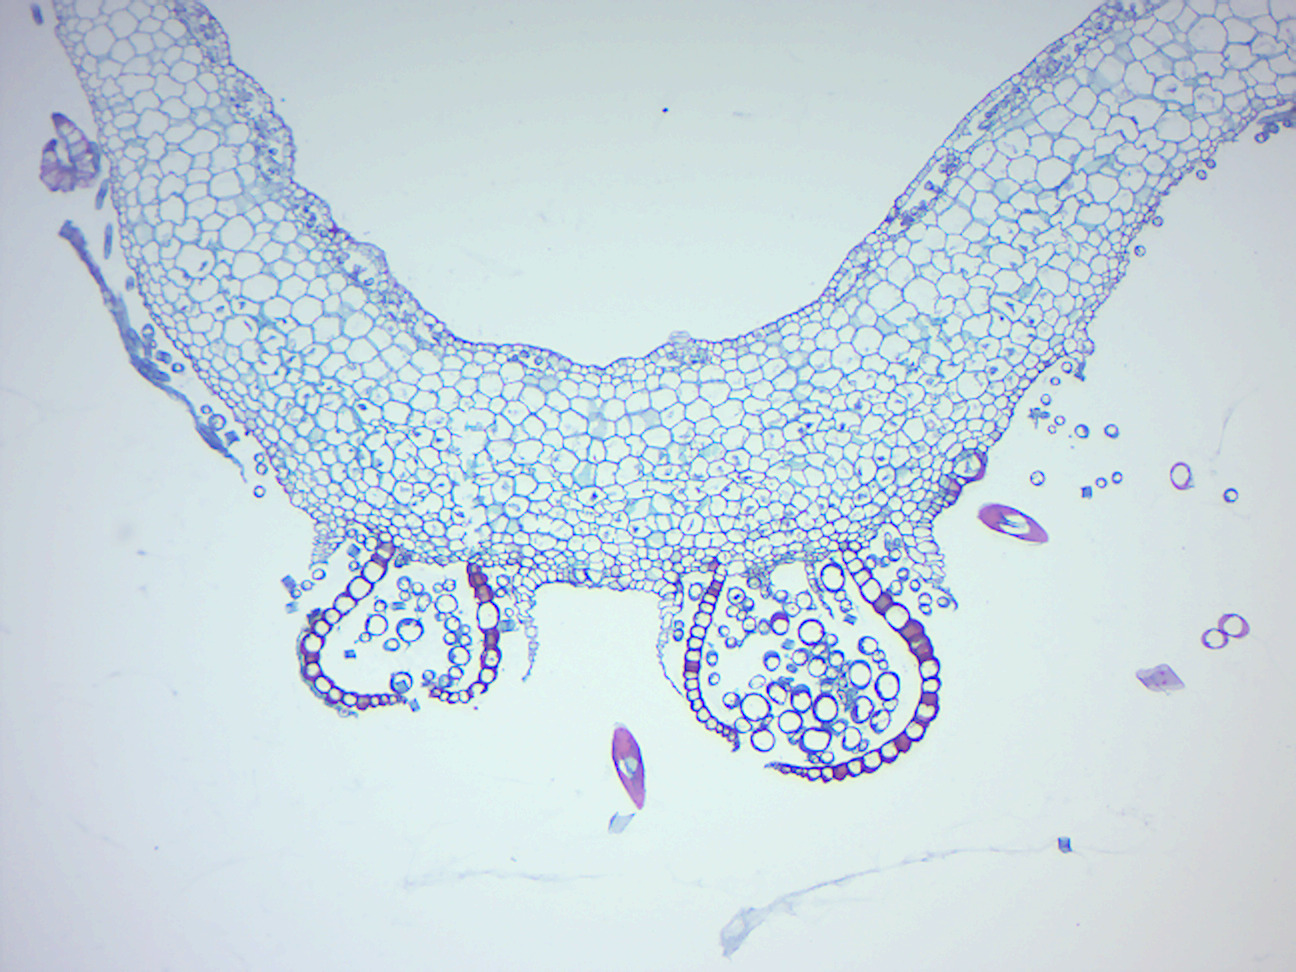
\includegraphics[width=0.7\linewidth]{./figures/mosses/marchantia_thallus}

}

\caption{\emph{Marchantia} thallus.}\label{fig:marchantiathallus}
\end{figure}

\begin{figure}

{\centering 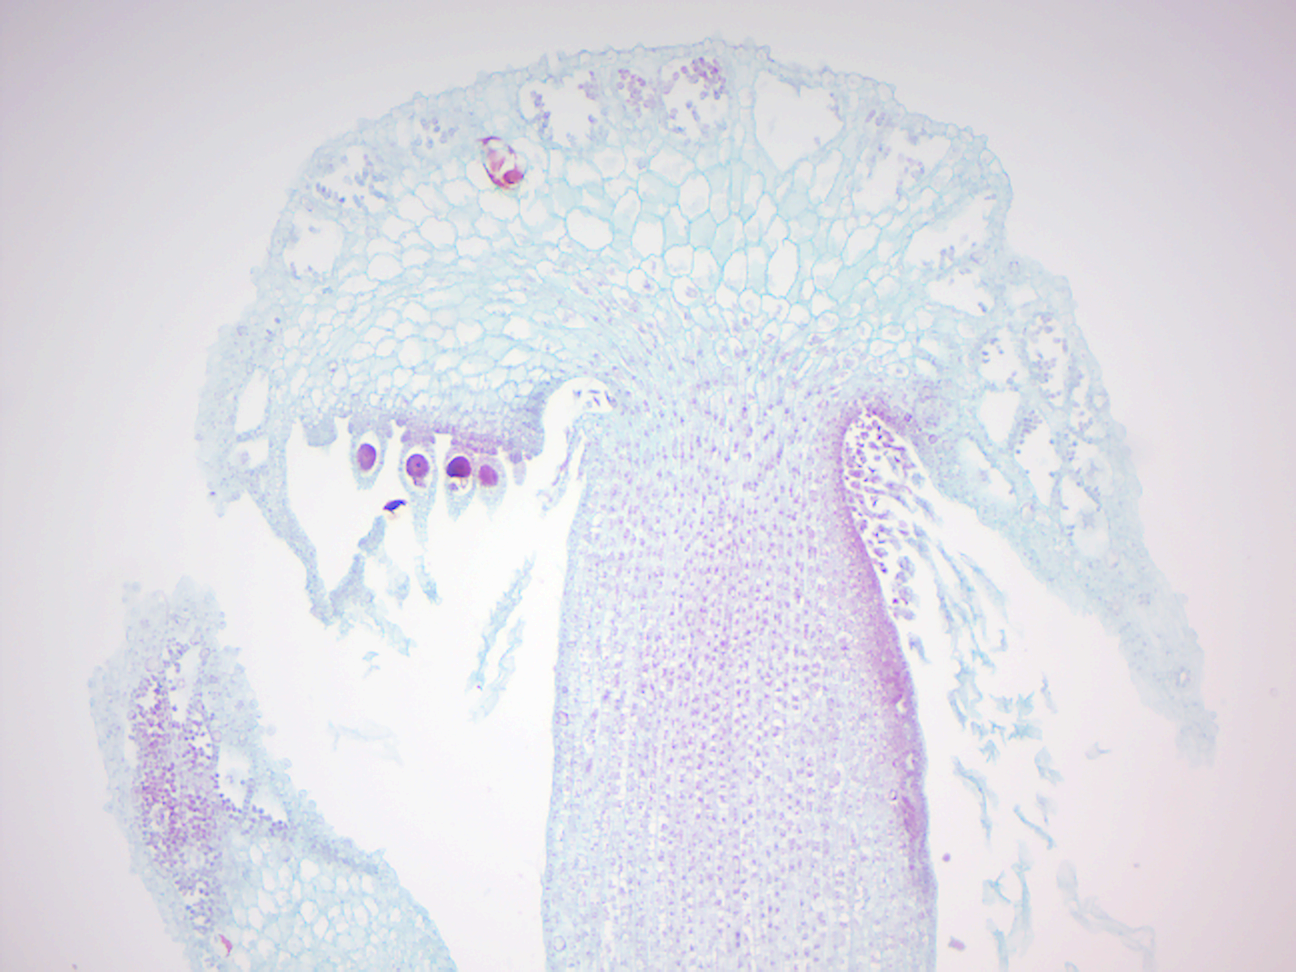
\includegraphics[width=0.7\linewidth]{./figures/mosses/marchantia_archegonia}

}

\caption{\emph{Marchantia} archegonia.}\label{fig:marchantiaarchegonia}
\end{figure}

\begin{figure}

{\centering 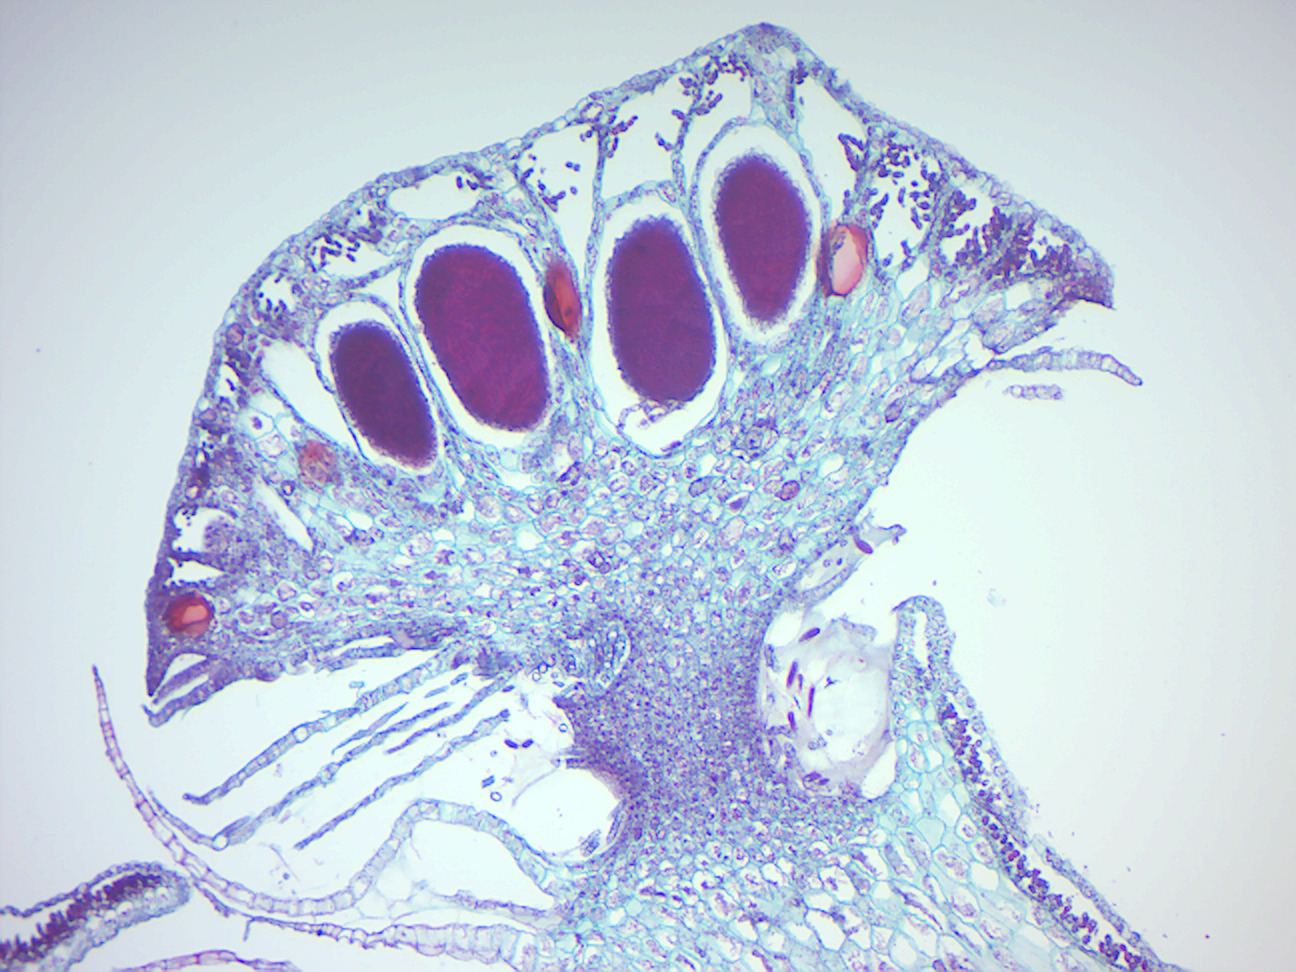
\includegraphics[width=0.7\linewidth]{./figures/mosses/marchantia_antheridia}

}

\caption{\emph{Marchantia} antheridia.}\label{fig:marchantiaantheridia}
\end{figure}

\begin{figure}

{\centering 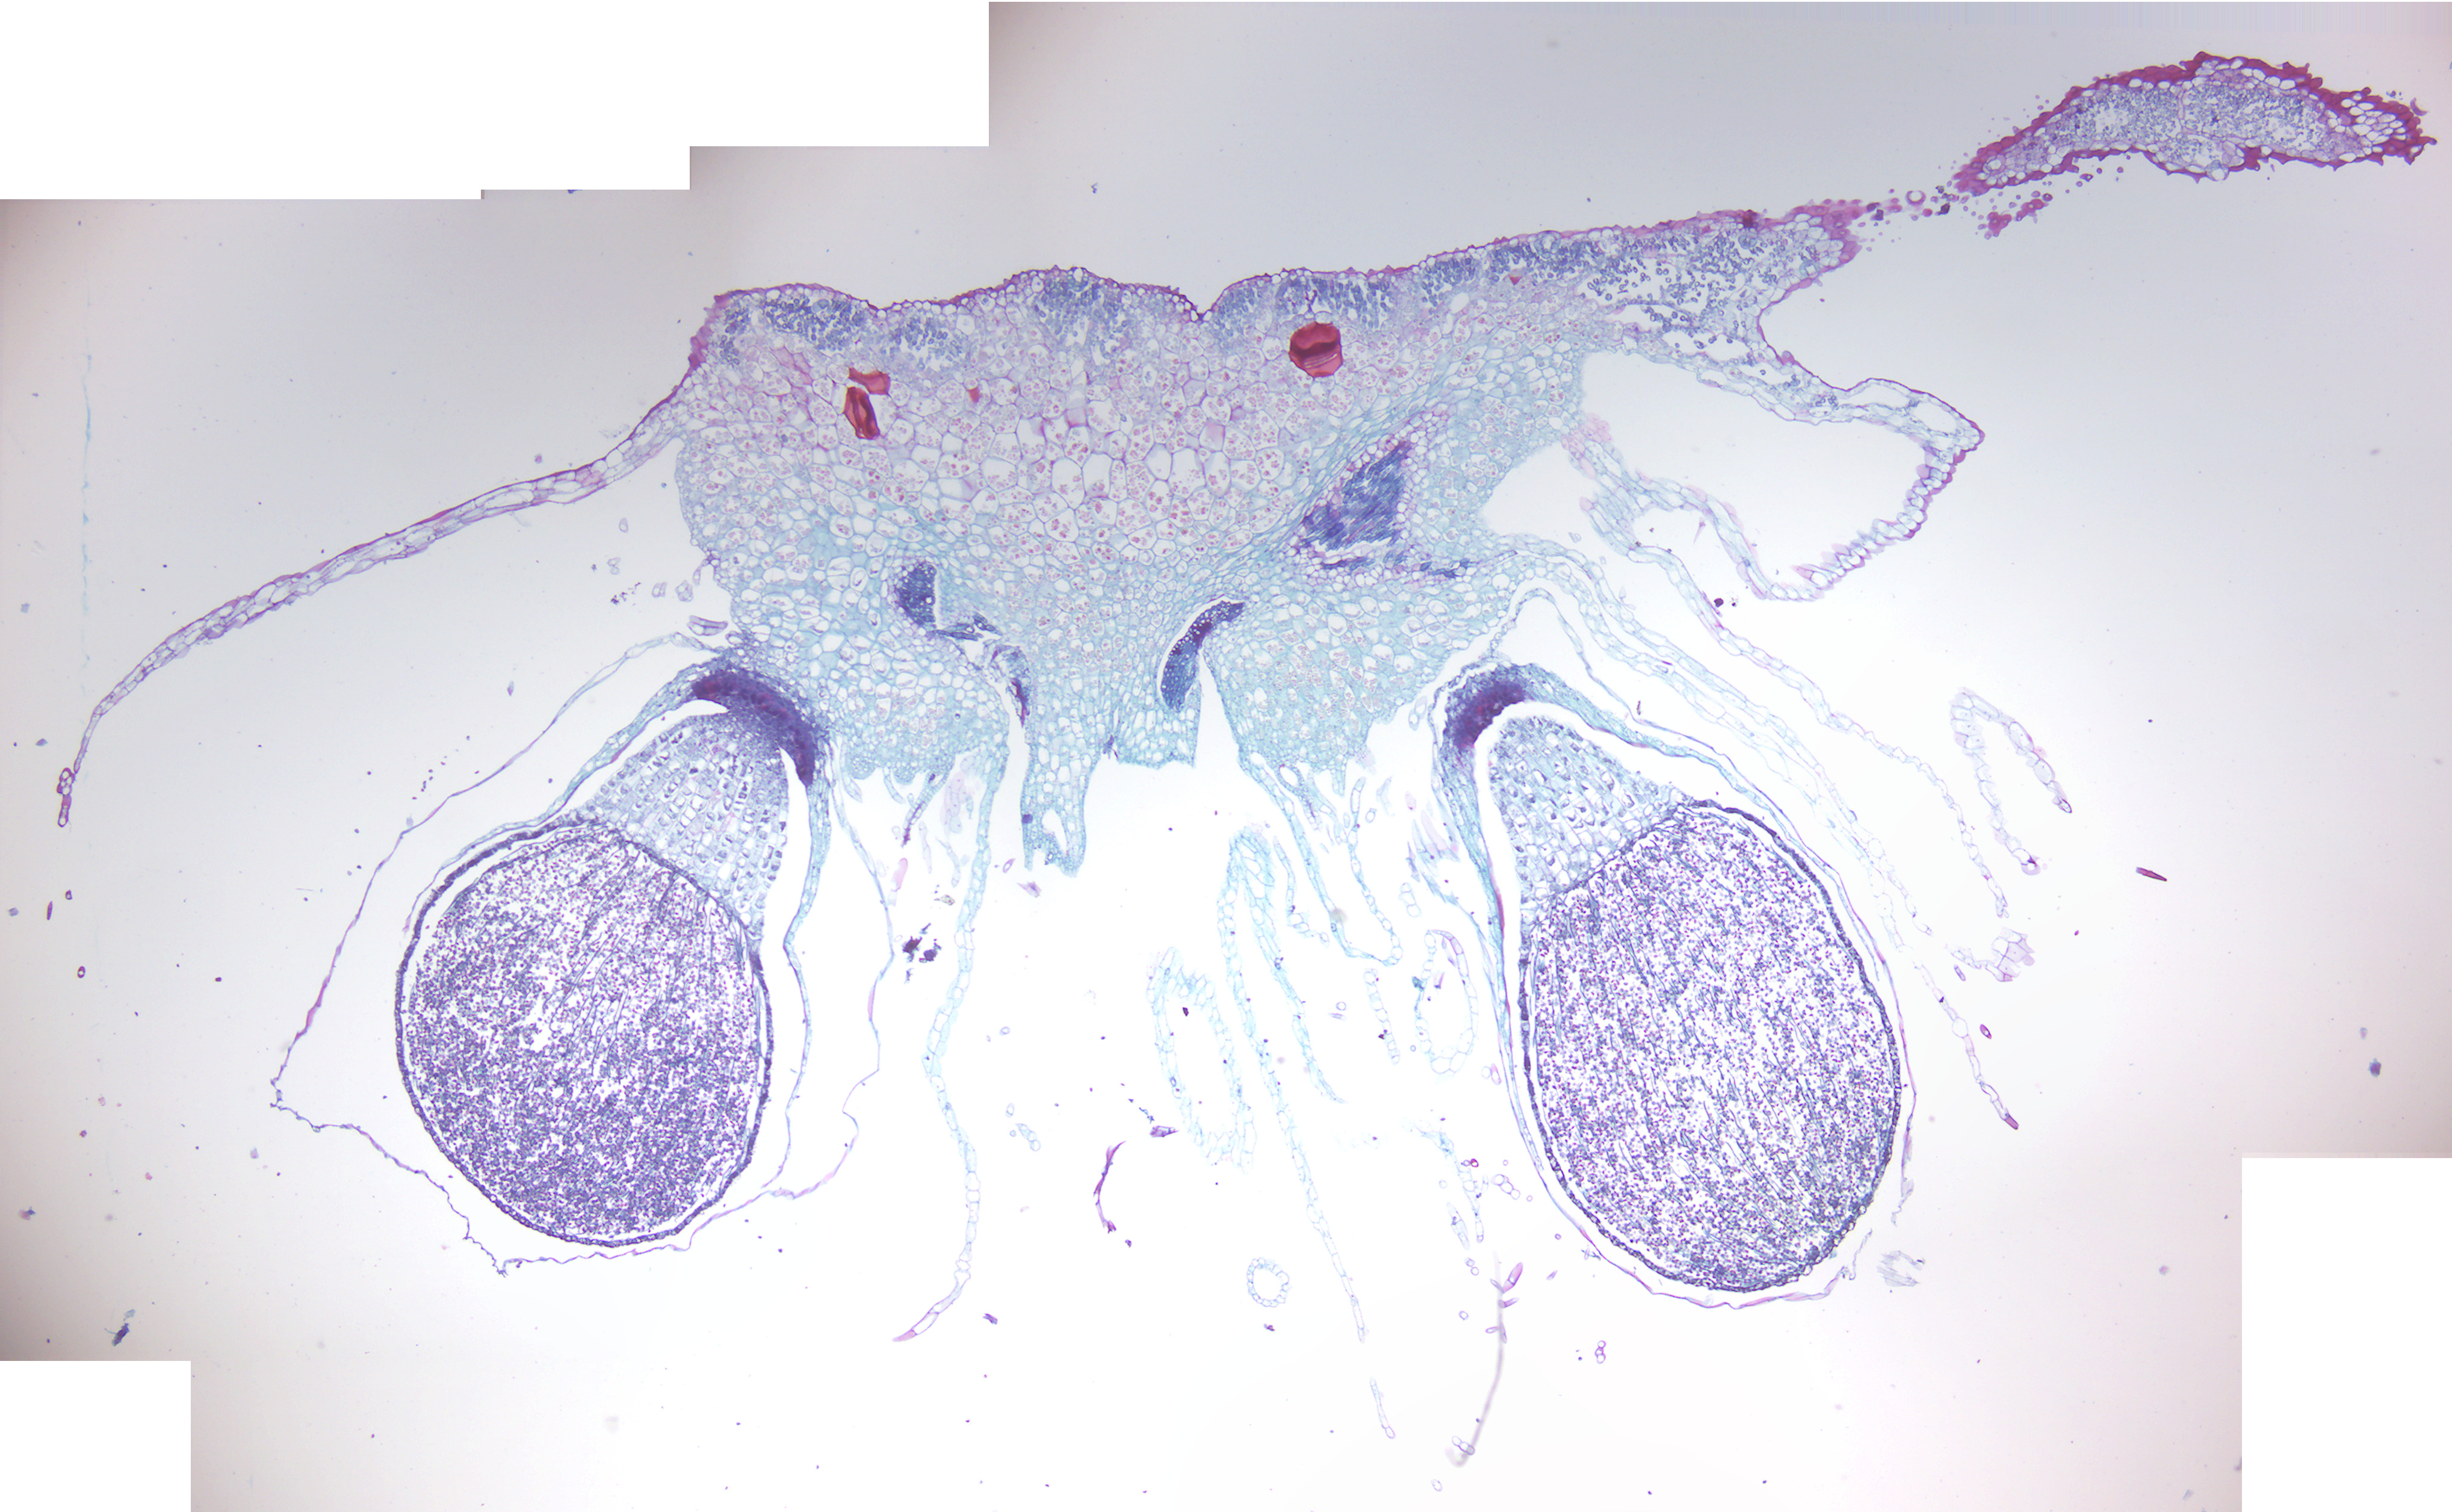
\includegraphics[width=0.7\linewidth]{./figures/mosses/marchantia_sporophyte}

}

\caption{\emph{Marchantia} sporophyte.}\label{fig:marchantiasporophyte}
\end{figure}

\begin{figure}

{\centering 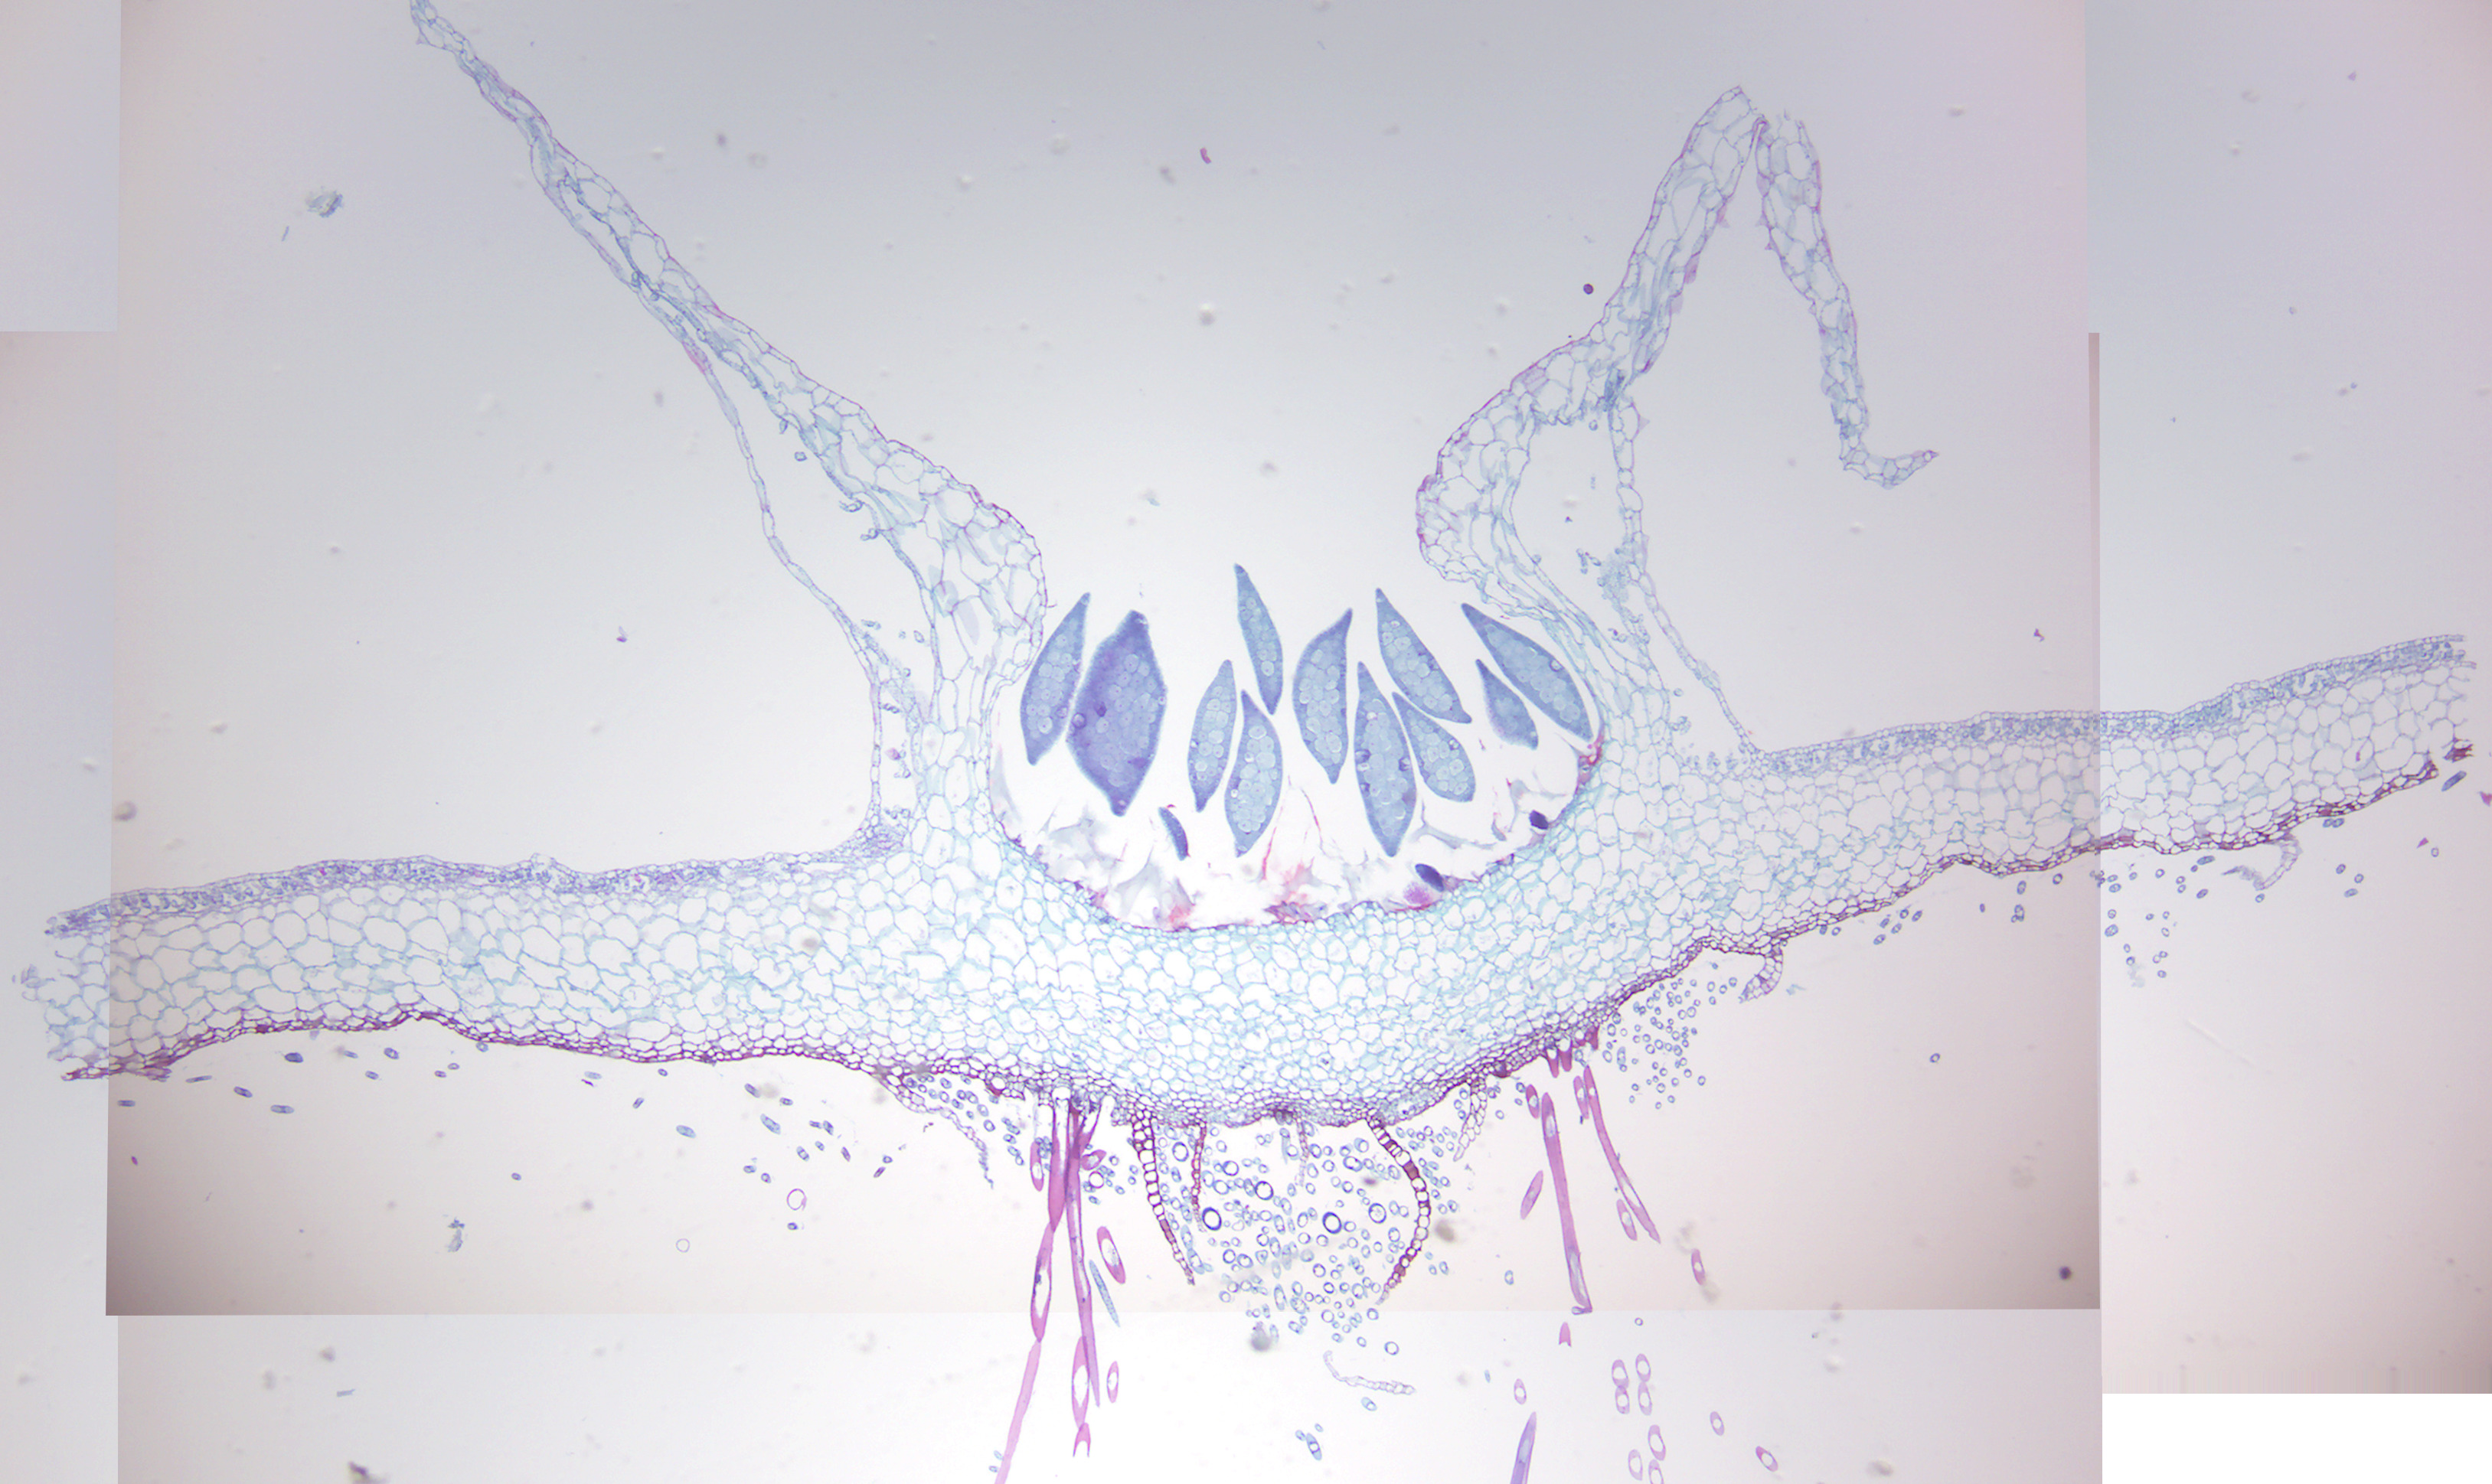
\includegraphics[width=0.7\linewidth]{./figures/mosses/marchantia_gemma_cup}

}

\caption{\emph{Marchantia} gemma cup.}\label{fig:gemma}
\end{figure}

\section{Vascular plants}\label{vascular-plants}

\href{https://en.wikipedia.org/wiki/Vascular_plant}{Vascular plants}
(from Latin vasculum: duct), also known as tracheophytes (from the
equivalent Greek term trachea) and also higher plants, form a large
group of plants (c. 308,312 accepted known species) that are defined as
those land plants that have lignified tissues (the xylem) for conducting
water and minerals throughout the plant. They also have a specialized
non-lignified tissue (the phloem) to conduct products of photosynthesis.
Vascular plants include the clubmosses, horsetails, ferns, gymnosperms
(including conifers) and angiosperms (flowering plants). Scientific
names for the group include Tracheophyta and Tracheobionta.

Vascular plants are distinguished by two primary characteristics:

\begin{enumerate}
\def\labelenumi{\arabic{enumi}.}
\tightlist
\item
  Vascular plants have vascular tissues which distribute resources
  through the plant. This feature allows vascular plants to evolve to a
  larger size than non-vascular plants, which lack these specialized
  conducting tissues and are therefore restricted to relatively small
  sizes.
\item
  In vascular plants, the principal generation phase is the sporophyte,
  which is usually diploid with two sets of chromosomes per cell. Only
  the germ cells and gametophytes are haploid. By contrast, the
  principal generation phase in non-vascular plants is the gametophyte,
  which is haploid with one set of chromosomes per cell. In these
  plants, only the spore stalk and capsule are diploid.
\end{enumerate}

Vascular plants first appeared during the Silurian period, and by the
Devonian had diversified and spread into many different terrestrial
environments. They developed a number of adaptations that allowed them
to spread into increasingly more arid places, notably the vascular
tissues xylem and phloem, that transport water and food throughout the
organism. Root systems capable of obtaining soil water and nutrients
also evolved during the Devonian. In modern vascular plants, the
sporophyte is typically large, branched, nutritionally independent and
long-lived, but there is increasing evidence that Paleozoic gametophytes
were just as complex as the sporophytes. The gametophytes of all
vascular plant groups evolved to become reduced in size and prominence
in the life cycle.

The first seed plants, pteridosperms (seed ferns), now extinct, appeared
in the Devonian and diversified through the Carboniferous. In these the
micro gametophyte is reduced to pollen and the mega gametophyte remains
inside the megasporangium, attached to the parent plant. A
megasporangium invested in protective layer called an integument is
known as an ovule. After fertilization by means of sperm deposited by
pollen grains, an embryo develops inside the ovule. The integument
becomes a seed coat, and the ovule develops into a seed. Seed plants can
survive and reproduce in extremely arid conditions, because they are not
dependent on free water for the movement of sperm, or the development of
free living gametophytes.

\section{Pteridophyta}\label{pteridophyta}

The \href{https://en.wikipedia.org/wiki/Pteridophyte}{pteridophytes} are
vascular plants (with xylem and phloem) that reproduces via spores, and
include the ferns, horsetails, and the lycophytes (clubmosses, spike
mosses, and quillworts). These are not a monophyletic group because
ferns and horsetails are more closely related to seed plants than to the
lycophytes. Therefore, ``Pteridophyta'' is now an invalid taxon,
although the term pteridophyte remains in common use.

\begin{figure}

{\centering 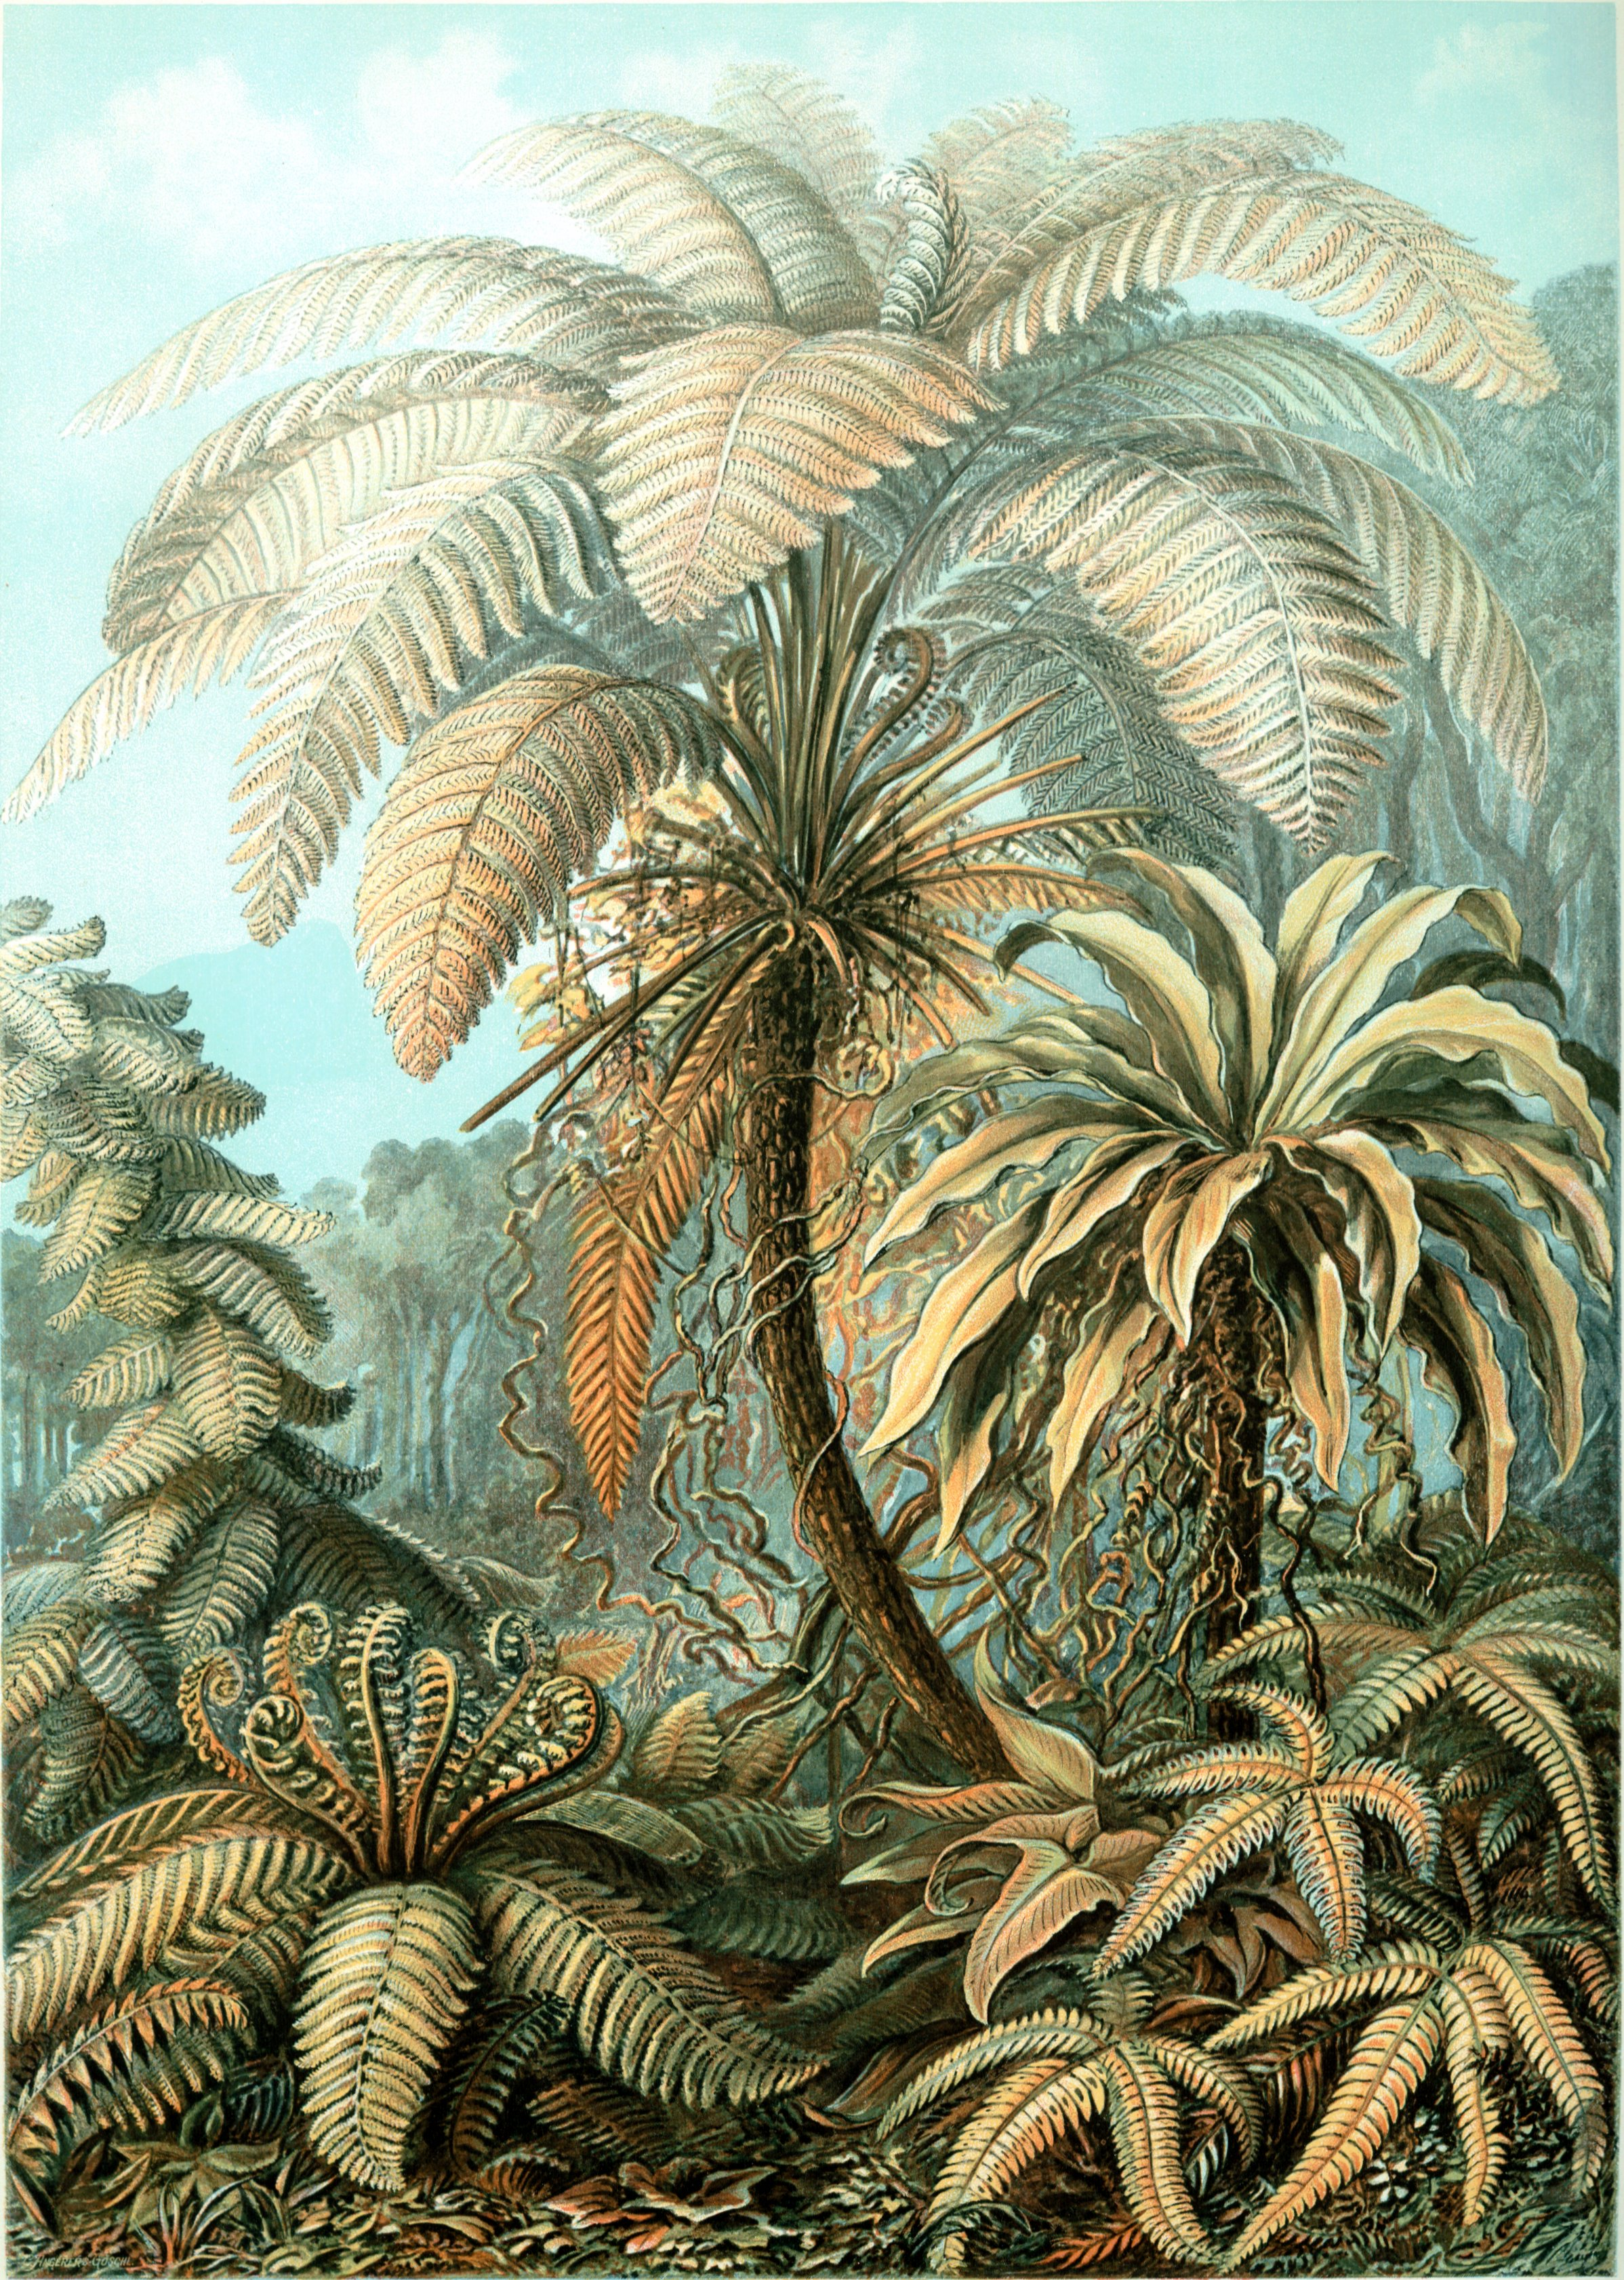
\includegraphics[width=0.7\linewidth]{./figures/mosses/Haeckel_Filicinae_92}

}

\caption{\href{https://commons.wikimedia.org/wiki/File:Haeckel_Filicinae_92.jpg}{Ferns}
from Ernst Haeckel's
\href{https://en.wikipedia.org/wiki/Kunstformen_der_Natur}{Kunstformen
der Natur}, 1904.}\label{fig:ferns}
\end{figure}

\subsection{Life cycle}\label{life-cycle-2}

Ferns are vascular plants differing from lycophytes by having true
leaves (megaphylls). They differ from seed plants (gymnosperms and
angiosperms) in their mode of reproduction---lacking flowers and seeds.
Like all land plants, they have a life cycle referred to as alternation
of generations, characterized by alternating diploid sporophytic and
haploid gametophytic phases. The diploid sporophyte has 2n paired
chromosomes, where n varies from species to species. The haploid
gametophyte has n unpaired chromosomes, i.e.~half the number of the
sporophyte. The gametophyte of ferns is a free-living organism, whereas
the gametophyte of the gymnosperms and angiosperms is dependent on the
sporophyte.

The life cycle of a typical fern proceeds as follows:

\begin{enumerate}
\def\labelenumi{\arabic{enumi}.}
\tightlist
\item
  A diploid sporophyte phase produces haploid spores by meiosis.
\item
  A spore grows into a haploid gametophyte by mitosis. The gametophyte
  typically consists of a photosynthetic prothallus.
\item
  The gametophyte produces gametes (often both sperm and eggs on the
  same prothallus) by mitosis.
\item
  A mobile, flagellate sperm fertilizes an egg that remains attached to
  the prothallus.
\item
  The fertilized egg is now a diploid zygote and grows by mitosis into a
  diploid sporophyte (the typical ``fern'' plant).
\end{enumerate}

\section{Clubmosses}\label{clubmosses}

\href{https://en.wikipedia.org/wiki/Lycopodiopsida}{Lycopodiopsida} is a
class of herbaceous vascular plants known as the clubmosses and
firmosses. They have dichotomously branching stems bearing simple leaves
without ligules and reproduce by means of spores borne in sporangia at
the bases of the leaves. Traditionally, the group also included the
spikemosses (Selaginella and relatives) and the quillworts (Isoetes and
relatives) but because these groups have leaves with ligules and
reproduce using spores of two different sizes both are now placed into
another class, Isoetopsida that also includes the extinct
Lepidodendrales. These groups, together with the horsetails are often
referred to informally as fern allies.

\section{Spikemosses}\label{spikemosses}

\href{https://en.wikipedia.org/wiki/Selaginella}{\emph{Selaginella}} is
the sole genus of primitive vascular plants in the family
Selaginellaceae, the spikemosses or lesser clubmosses. Selaginella
occurs mostly in the tropical regions of the world, with a handful of
species to be found in the arctic-alpine zones of both hemispheres.

\section{View Prepared Slides of
Selaginella}\label{view-prepared-slides-of-selaginella}

\begin{enumerate}
\def\labelenumi{\arabic{enumi}.}
\tightlist
\item
  \emph{Selaginella} strobilus (Figure \ref{fig:selaginstrobilus})

  \begin{itemize}
  \tightlist
  \item
    Identify: micro- and megaspores
  \end{itemize}
\end{enumerate}

\begin{figure}

{\centering 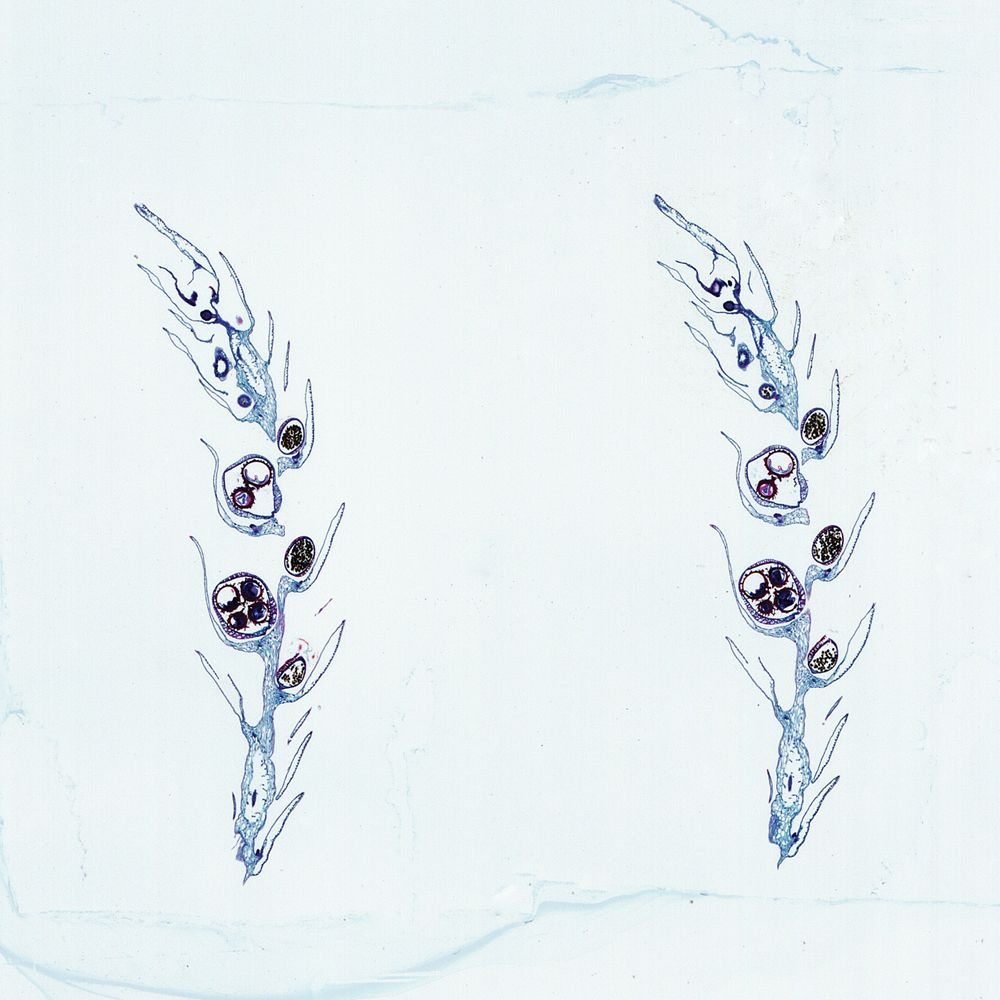
\includegraphics[width=0.7\linewidth]{./figures/mosses/selaginella_strobilus}

}

\caption{Selaginella strobilus.}\label{fig:selaginstrobilus}
\end{figure}

\section{Horsetails}\label{horsetails}

\href{https://en.wikipedia.org/wiki/Equisetum}{\emph{Equisetum}}
(horsetail) is the only living genus in Equisetaceae, a family of
vascular plants that reproduce by spores rather than seeds. \emph{Equisetum} is
a ``living fossil'' as it is the only living genus of the entire class
Equisetopsida, which for over one hundred million years was much more
diverse and dominated the understory of late Paleozoic forests. Some
Equisetopsida were large trees reaching to 30 meters tall.

\section{View Prepared Slides of
\emph{Equisetum}}\label{view-prepared-slides-of-equisetum}

\begin{enumerate}
\def\labelenumi{\arabic{enumi}.}
\tightlist
\item
  \emph{Equisetum} strobilus (Figure \ref{fig:equisetumstrobilus})

  \begin{itemize}
  \tightlist
  \item
    Identify: sporangiphores and spores
  \end{itemize}
\end{enumerate}

\begin{figure}

{\centering 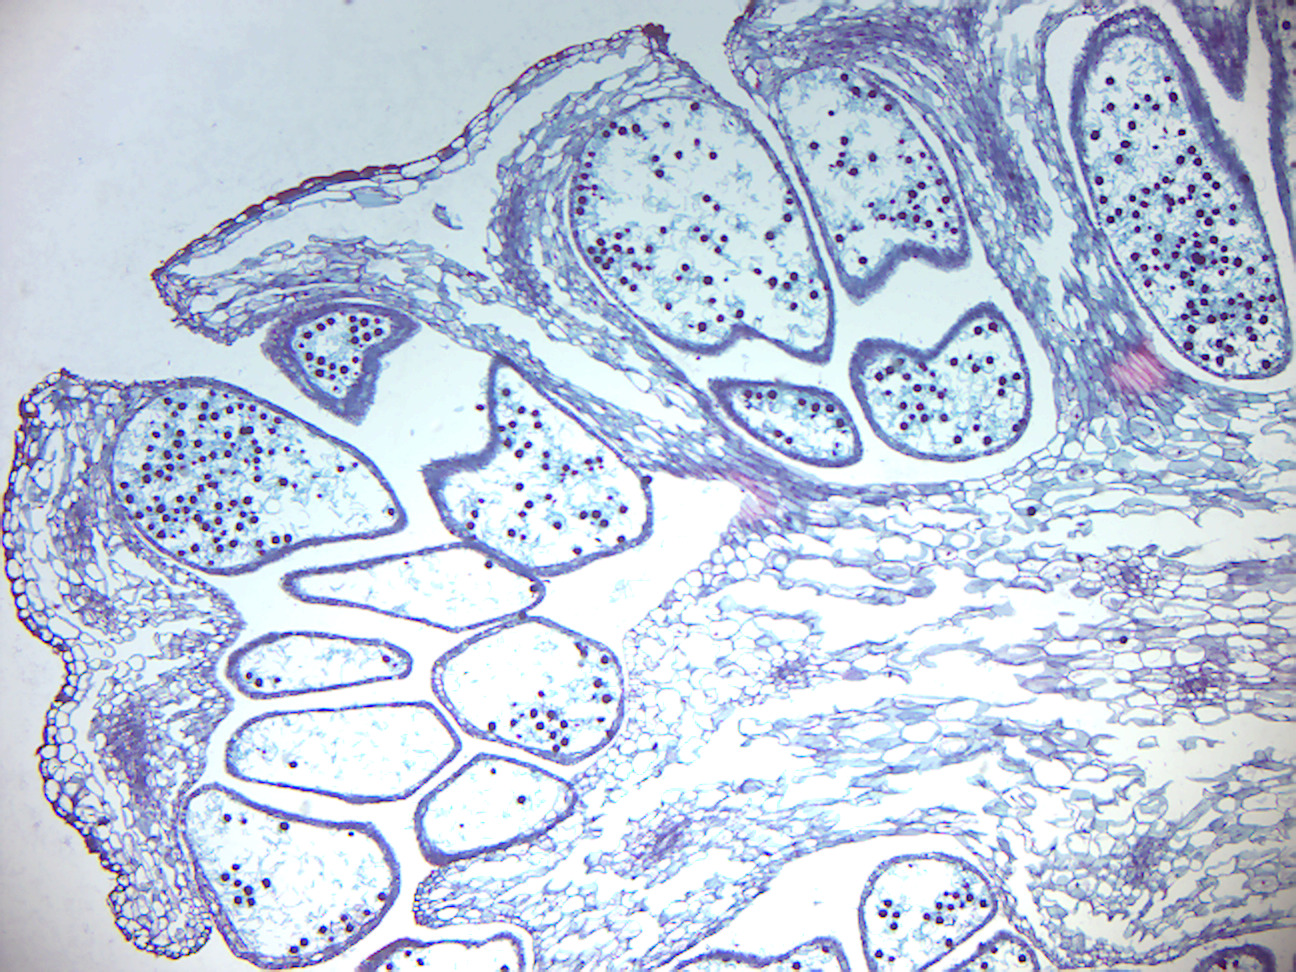
\includegraphics[width=0.7\linewidth]{./figures/mosses/equisetum_strobilus}

}

\caption{\emph{Equisetum} strobilus.}\label{fig:equisetumstrobilus}
\end{figure}

\section{Whisk ferns}\label{whisk-ferns}

\href{https://en.wikipedia.org/wiki/Psilotum}{\emph{Psilotum}} is a genus of
fern-like vascular plants, commonly known as whisk ferns. It is one of
two genera in the family Psilotaceae, the other being Tmesipteris. They
lack true roots and leaves, the stems being the organs containing
conducting tissue.

\section{View Prepared Slides of
\emph{Psilotum}}\label{view-prepared-slides-of-psilotum}

\begin{enumerate}
\def\labelenumi{\arabic{enumi}.}
\tightlist
\item
  \emph{Psilotum} sporangium (Figure \ref{fig:psilotumsporangium})

  \begin{itemize}
  \tightlist
  \item
    Identify: Sporangium, spores.
  \end{itemize}
\end{enumerate}

\begin{figure}

{\centering 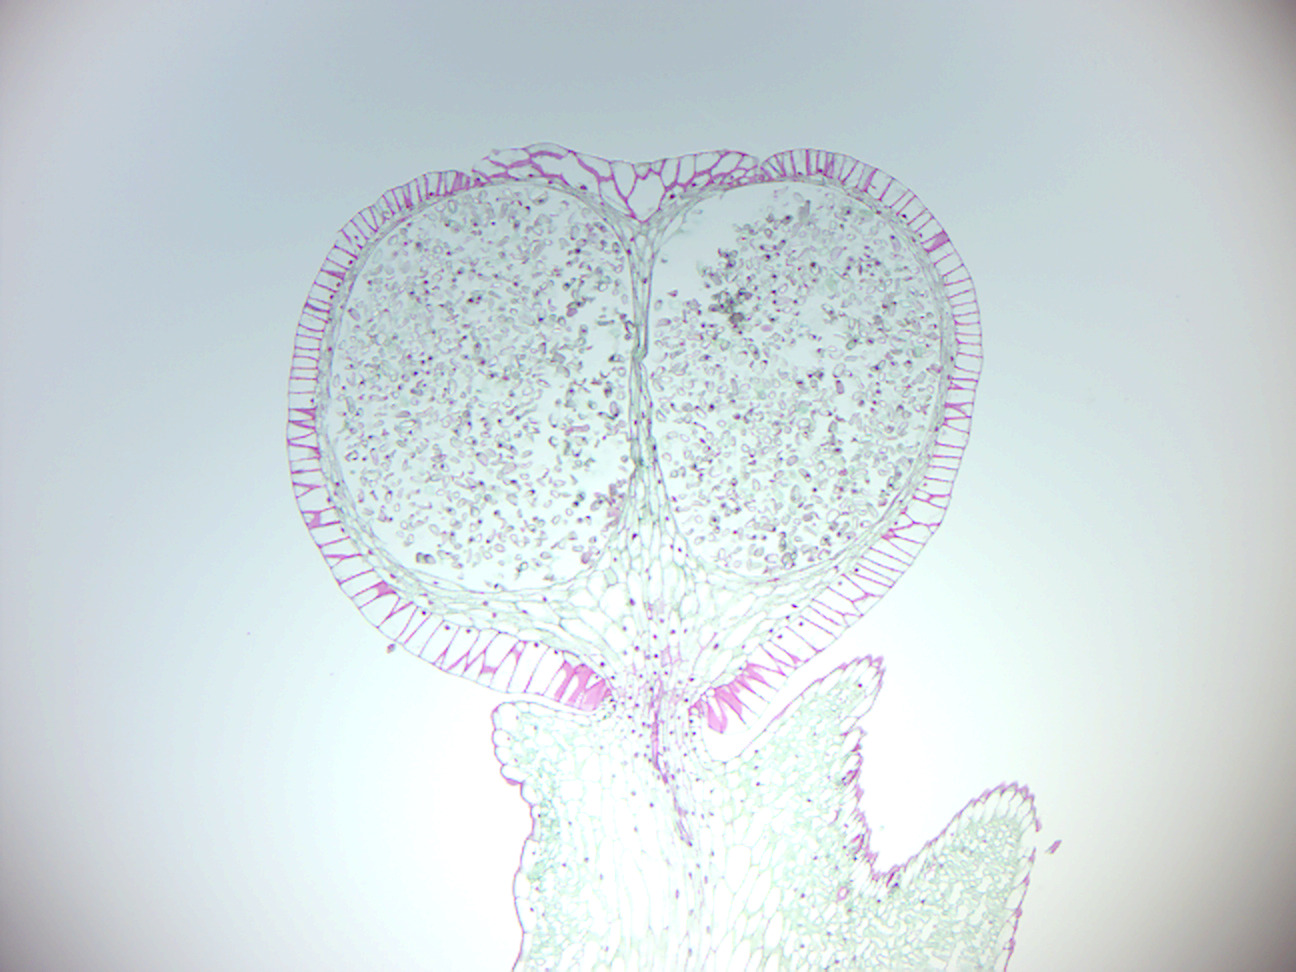
\includegraphics[width=0.7\linewidth]{./figures/mosses/psilotum_sporangium}

}

\caption{\emph{Psilotum} sporangium.}\label{fig:psilotumsporangium}
\end{figure}

\section{View Prepared Slides of
Ferns}\label{view-prepared-slides-of-ferns}

\begin{enumerate}
\def\labelenumi{\arabic{enumi}.}
\tightlist
\item
  Fern sporophyte (Figure \ref{fig:fernsporophyte})
\item
  Fern antheridia \& archegonia (Figure \ref{fig:ferngametophyte})

  \begin{itemize}
  \tightlist
  \item
    Identify: tissue of the gametophyte; antheridia; archegonia;
    rhizoids
  \end{itemize}
\item
  Fern prothallus young sporophyte (Figure \ref{fig:fernprothallus})

  \begin{itemize}
  \tightlist
  \item
    Identify: sporophyte, gametophyte; rhizoids
  \end{itemize}
\end{enumerate}

\begin{figure}

{\centering 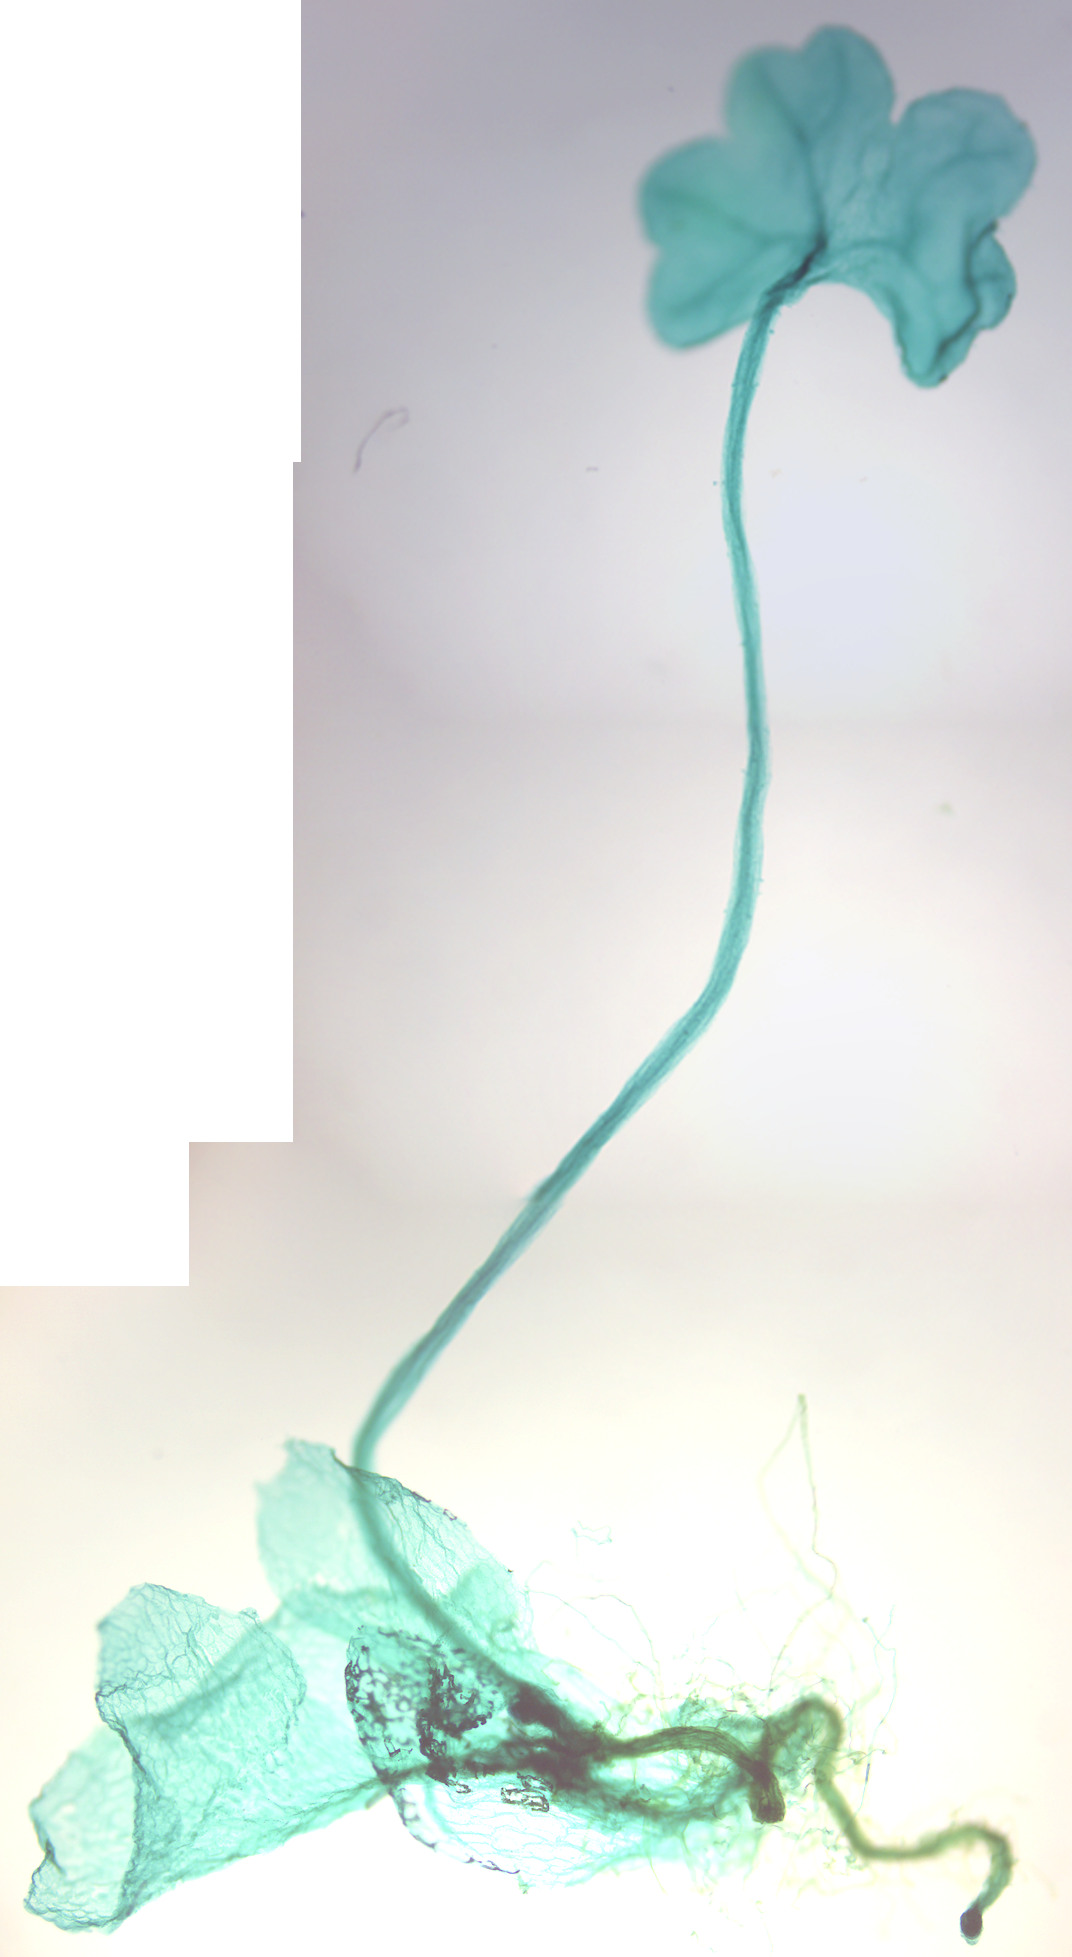
\includegraphics[width=0.7\linewidth]{./figures/mosses/fern_sporophyte}

}

\caption{Fern sporophyte.}\label{fig:fernsporophyte}
\end{figure}

\begin{figure}

{\centering 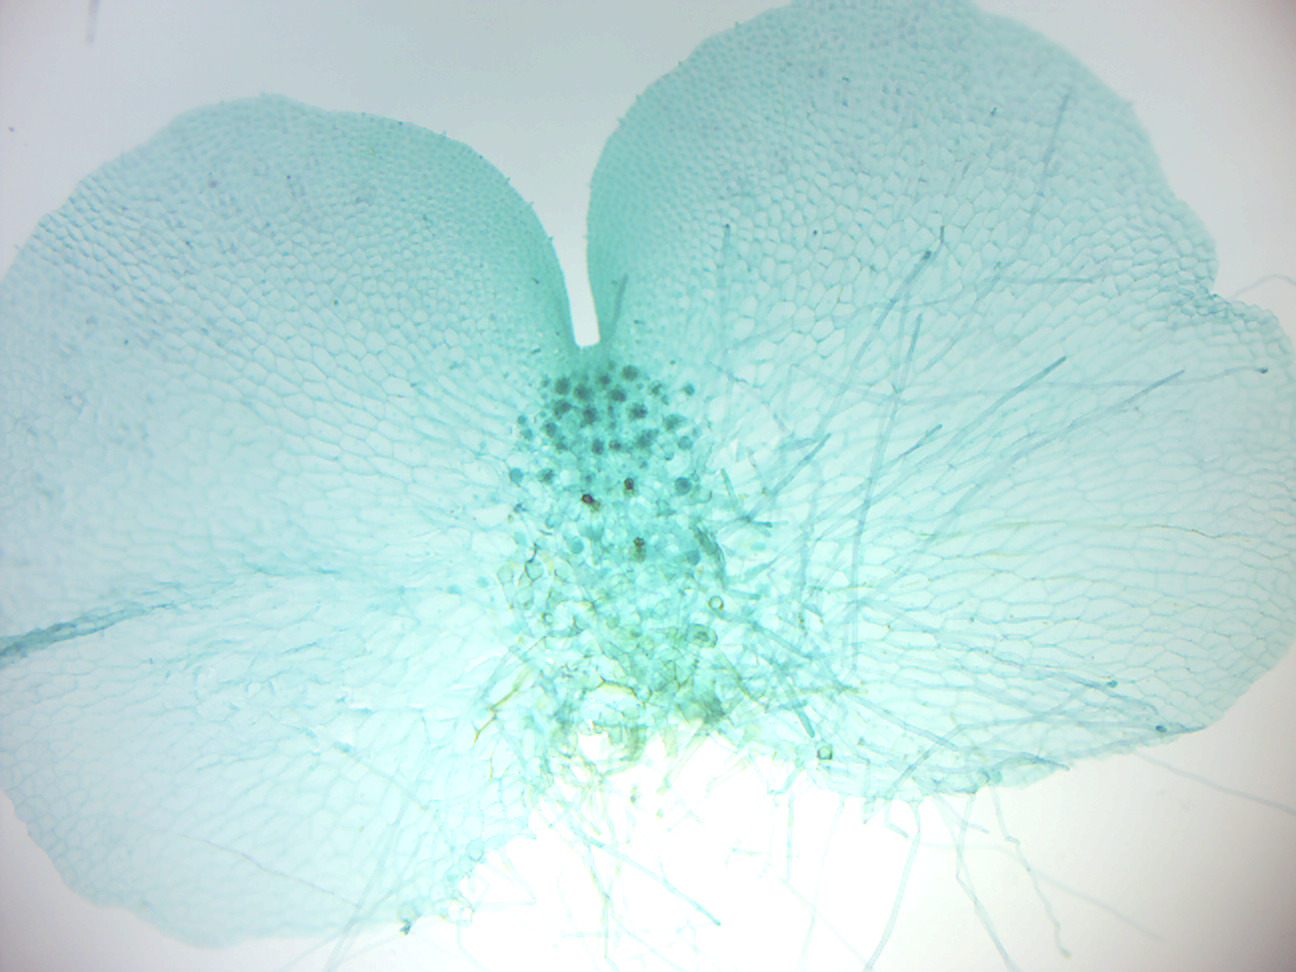
\includegraphics[width=0.7\linewidth]{./figures/mosses/fern_antheridia_archegonia}

}

\caption{Fern antheridia and archegonia.}\label{fig:ferngametophyte}
\end{figure}

\begin{figure}

{\centering 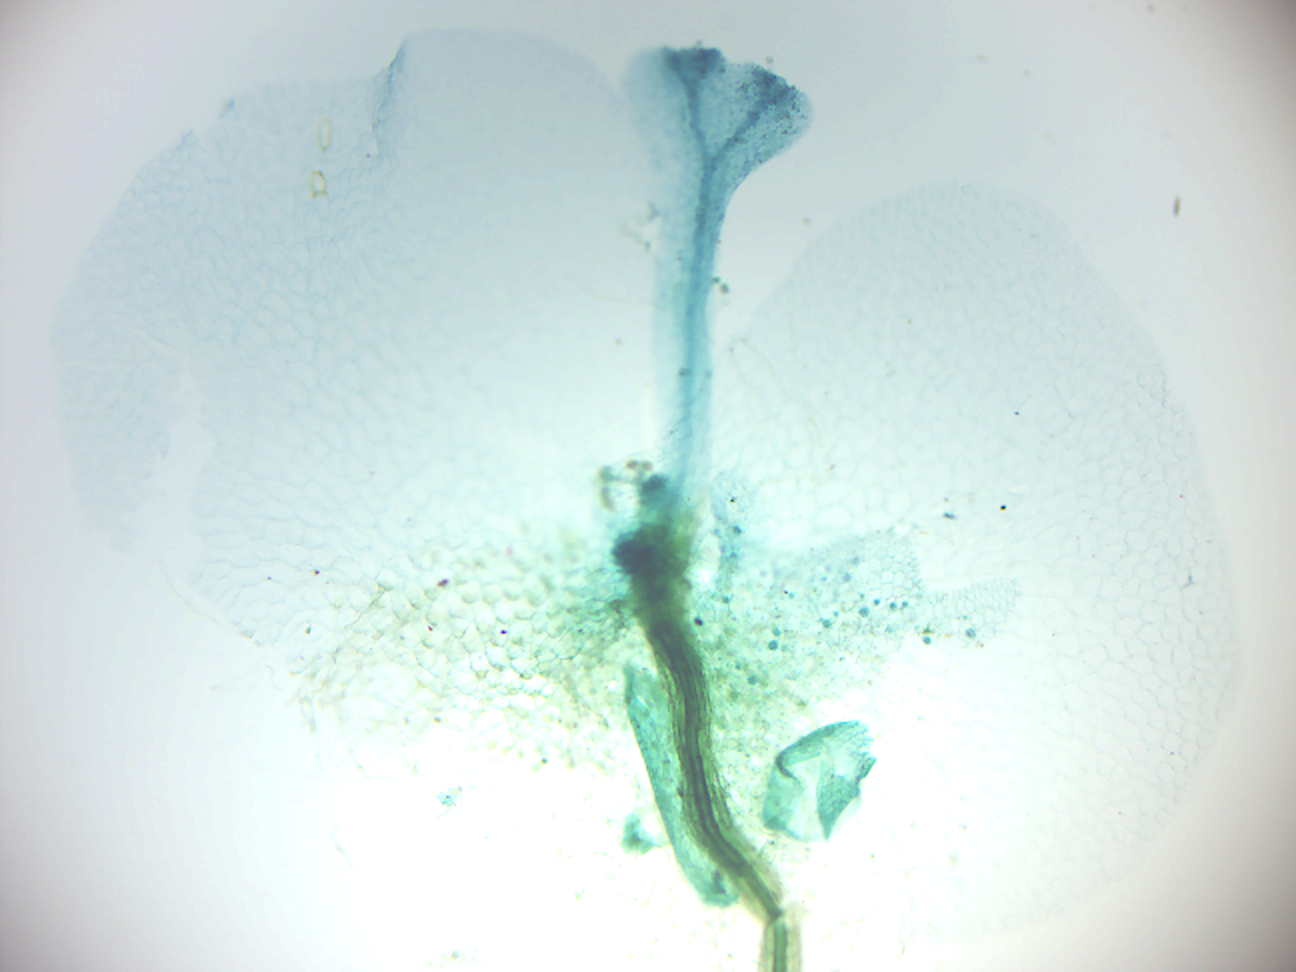
\includegraphics[width=0.7\linewidth]{./figures/mosses/fern_prothallus}

}

\caption{Fern prothallus young sporophyte.}\label{fig:fernprothallus}
\end{figure}

\section{View Prepared Slides of
\emph{Cyrtomium}}\label{view-prepared-slides-of-cyrtomium}

\href{https://en.wikipedia.org/wiki/Cyrtomium}{\emph{Cyrtomium}} is a
genus of about 15-20 species of ferns in the family Dryopteridaceae,
native to Asia, Africa (including Madagascar), and the Pacific Ocean
islands (Hawaii). \emph{Cyrtomium falcatum} is a species of fern known by the
common names house holly-fern and Japanese holly fern. It is native to
eastern Asia. It grows from crevices, coastal cliffs, streambanks, rocky
slopes, and other moist, stable areas.

\begin{enumerate}
\def\labelenumi{\arabic{enumi}.}
\tightlist
\item
  \emph{Cyrtomium falcatum} sorus on leaf

  \begin{itemize}
  \tightlist
  \item
    Locate sorus and identify the following: sporangia with spores
    inside; annular cells (annulus); lip cells; indusium (covering of
    the sorus).
  \end{itemize}
\end{enumerate}

\begin{figure}

{\centering 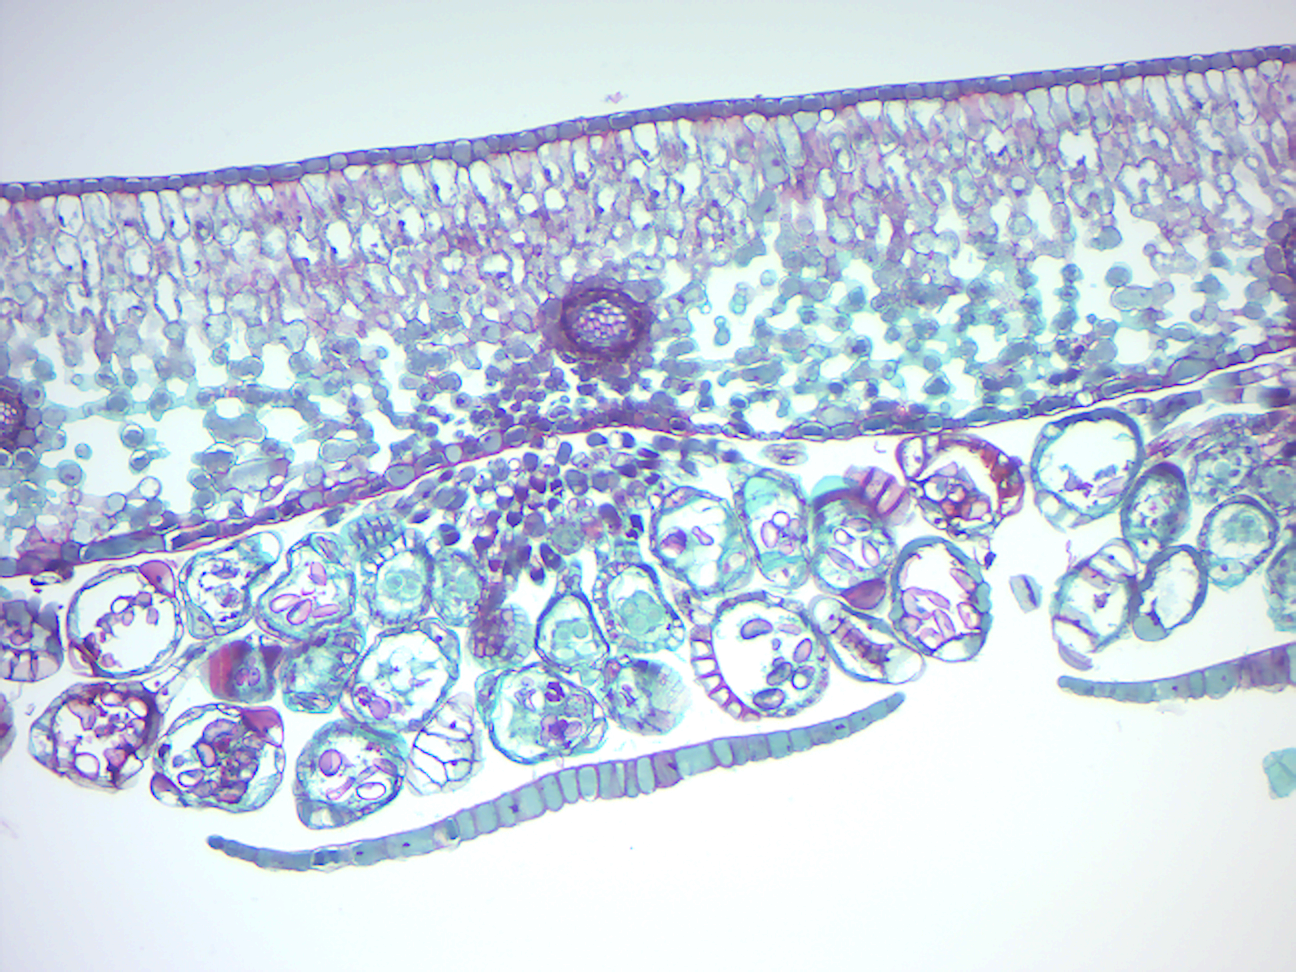
\includegraphics[width=0.7\linewidth]{./figures/mosses/cyrtomium_sorus}

}

\caption{\emph{Cyrtomium} falcatum sorus on leaf.}\label{fig:cyrtomium}
\end{figure}

\section{View Living Organisms}\label{view-living-organisms-1}

\begin{enumerate}
\def\labelenumi{\arabic{enumi}.}
\tightlist
\item
  Four types of Mosses
\item
  \emph{Marchantia hepatica}
\item
  \emph{Lycopodium lucidulum}
\end{enumerate}

\section{Review Questions}\label{review-questions-1}

\begin{enumerate}
\def\labelenumi{\arabic{enumi}.}
\tightlist
\item
  What are plants?
\item
  What are mosses?
\item
  What are liverworts?
\item
  What are ferns?
\item
  What does alternation of generations mean in the life cycle of plants?
\item
  What is a gametophyte?
\item
  What is a sporophyte?
\end{enumerate}

\chapter{Gymnosperms and Angiosperms}\label{gymnosperms-and-angiosperms}

The gymnosperms and angiosperms together compose the spermatophytes or
seed plants.

\section{Gymnosperms}\label{gymnosperms}

The \href{https://en.wikipedia.org/wiki/Gymnosperm}{gymnosperms} are a
group of seed-producing plants (spermatophytes) that includes conifers
(Pinophyta), cycads, Ginkgo, and gnetophytes. The term ``gymnosperm''
comes from the Greek composite word gymnos, ``naked'' and sperma,
``seed'', meaning ``naked seeds''. The name is based on the unenclosed
condition of their seeds (called ovules in their unfertilized state).
The non-encased condition of their seeds stands in contrast to the seeds
and ovules of flowering plants (angiosperms), which are enclosed within
an ovary. Gymnosperm seeds develop either on the surface of scales or
leaves, which are often modified to form cones, or solitary as in Yew,
Torreya, Ginkgo. By far the largest group of living gymnosperms are the
conifers (pines, cypresses, and relatives), followed by cycads,
gnetophytes (\emph{Gnetum}, \emph{Ephedra} and \emph{Welwitschia}), and \emph{Ginkgo biloba} (a
single living species). Roots in some genera have fungal association
with roots in the form of mycorrhiza (\emph{Pinus}), while in some others
(\emph{Cycas}) small specialized roots called coralloid roots are associated
with nitrogen-fixing cyanobacteria.

Gymnosperms, like all vascular plants, have a sporophyte-dominant life
cycle, which means they spend most of their life cycle with diploid
cells, while the gametophyte (gamete-bearing phase) is relatively
short-lived. Two spore types, microspores and megaspores, are typically
produced in pollen cones or ovulate cones, respectively. Gametophytes,
as with all heterosporous plants, develop within the spore wall. Pollen
grains (microgametophytes) mature from microspores, and ultimately
produce sperm cells. Megagametophytes develop from megaspores and are
retained within the ovule. Gymnosperms produce multiple archegonia,
which produce the female gamete. During pollination, pollen grains are
physically transferred between plants from the pollen cone to the ovule.
Pollen is usually moved by wind or insects. Whole grains enter each
ovule through a microscopic gap in the ovule coat (integument) called
the micropyle. The pollen grains mature further inside the ovule and
produce sperm cells. Two main modes of fertilization are found in
gymnosperms. Cycads and Ginkgo have motile sperm that swim directly to
the egg inside the ovule, whereas conifers and gnetophytes have sperm
with no flagella that are moved along a pollen tube to the egg. After
syngamy (joining of the sperm and egg cell), the zygote develops into an
embryo (young sporophyte). More than one embryo is usually initiated in
each gymnosperm seed. The mature seed comprises the embryo and the
remains of the female gametophyte, which serves as a food supply, and
the seed coat.

\section{View Prepared Slides of
Gymnosperms}\label{view-prepared-slides-of-gymnosperms}

\begin{enumerate}
\def\labelenumi{\arabic{enumi}.}
\tightlist
\item
  \emph{Zamia} young ovule (Figure \ref{fig:zamia})
\item
  Pine ovule (Figure \ref{fig:pine})

  \begin{itemize}
  \tightlist
  \item
    Identify: female gametophyte, egg, archegonia, micropyle
  \end{itemize}
\item
  Pine young ovulate cone (Figure \ref{fig:ovulate})

  \begin{itemize}
  \tightlist
  \item
    Identify: ovules, megasporophylls (scales)
  \end{itemize}
\item
  Pine staminate cone (Figure \ref{fig:staminate})

  \begin{itemize}
  \tightlist
  \item
    Identify: microsporophyll, microsporangium, pollen grains
    (microspores). In pollen grains, differentiate between the cells and
    the ``wings''
  \end{itemize}
\item
  Pine pollen (Figure \ref{fig:pollen})

  \begin{itemize}
  \tightlist
  \item
    Identify: generative cell with nucleus, tube cell with nucleus,
    ``wings''
  \end{itemize}
\item
  Pine - mature embryo
\item
  Pine needle (Figure \ref{fig:needle})

  \begin{itemize}
  \tightlist
  \item
    Identify: epidermis, stomata with guard cells, hypodermis,
    mesophyll, resin canals, endodermis, xylem, and phloem
  \end{itemize}
\end{enumerate}

\begin{figure}

{\centering \includegraphics[width=0.7\linewidth]{./figures/gymnosperms/zamia}

}

\caption{Young \emph{Zamia} ovule.}\label{fig:zamia}
\end{figure}

\begin{figure}

{\centering 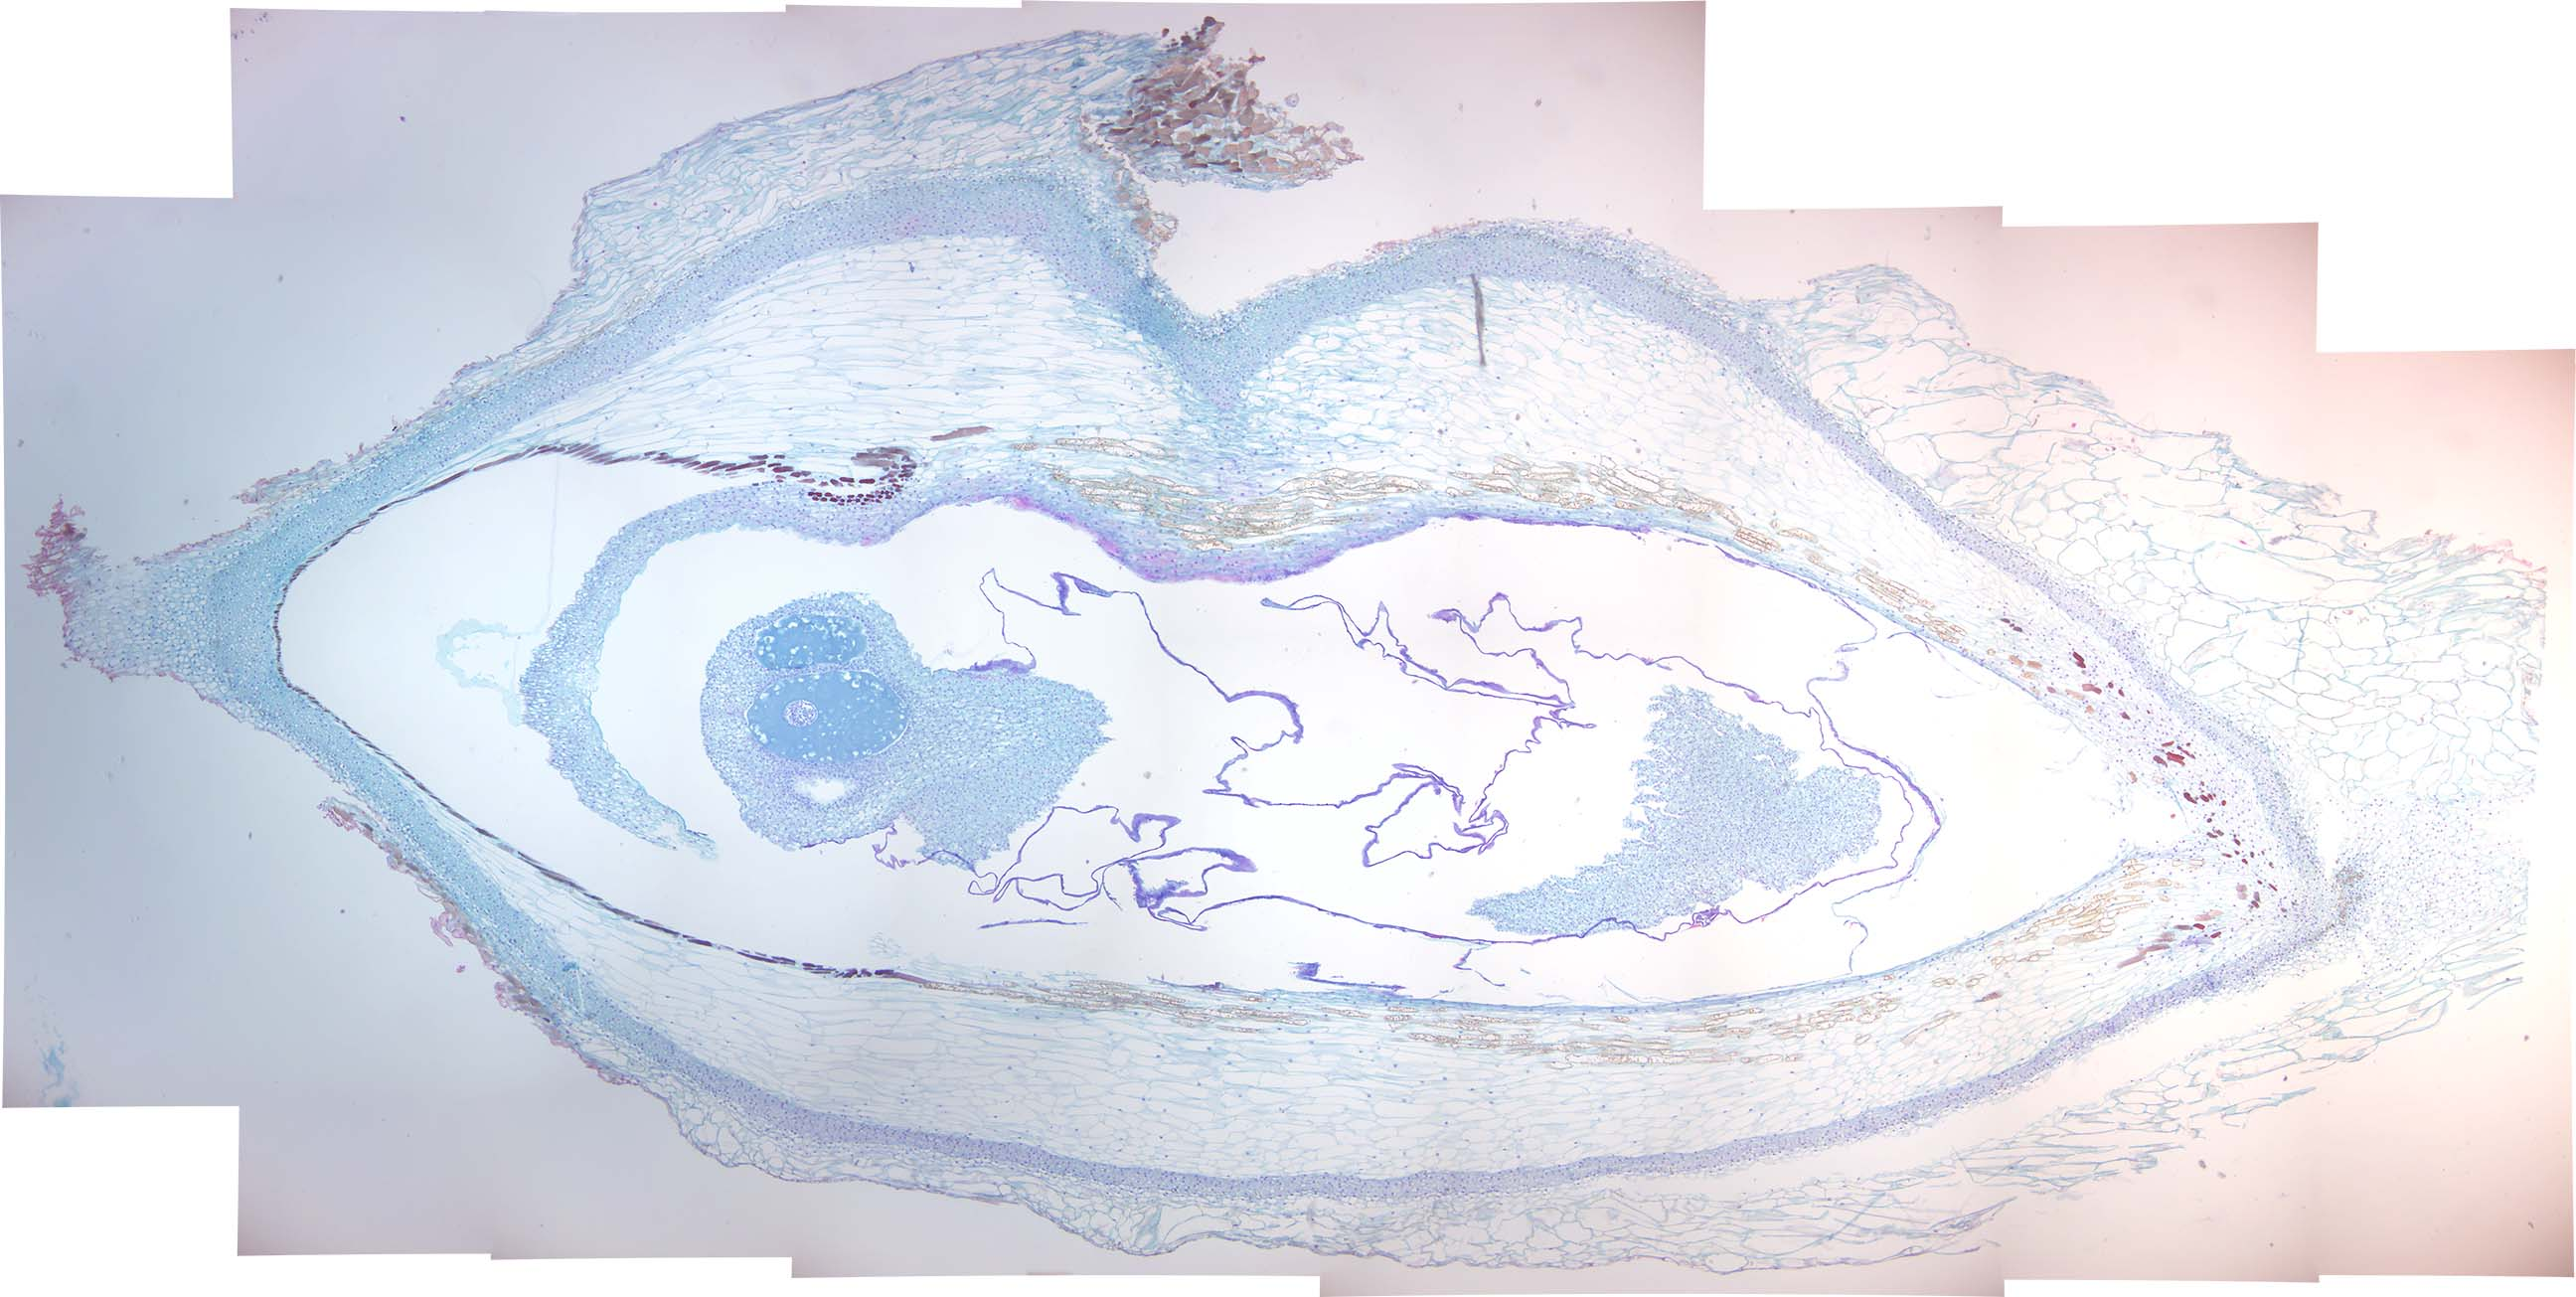
\includegraphics[width=0.7\linewidth]{./figures/gymnosperms/pine_ovule}

}

\caption{Pine ovule}\label{fig:pine}
\end{figure}

\begin{figure}

{\centering 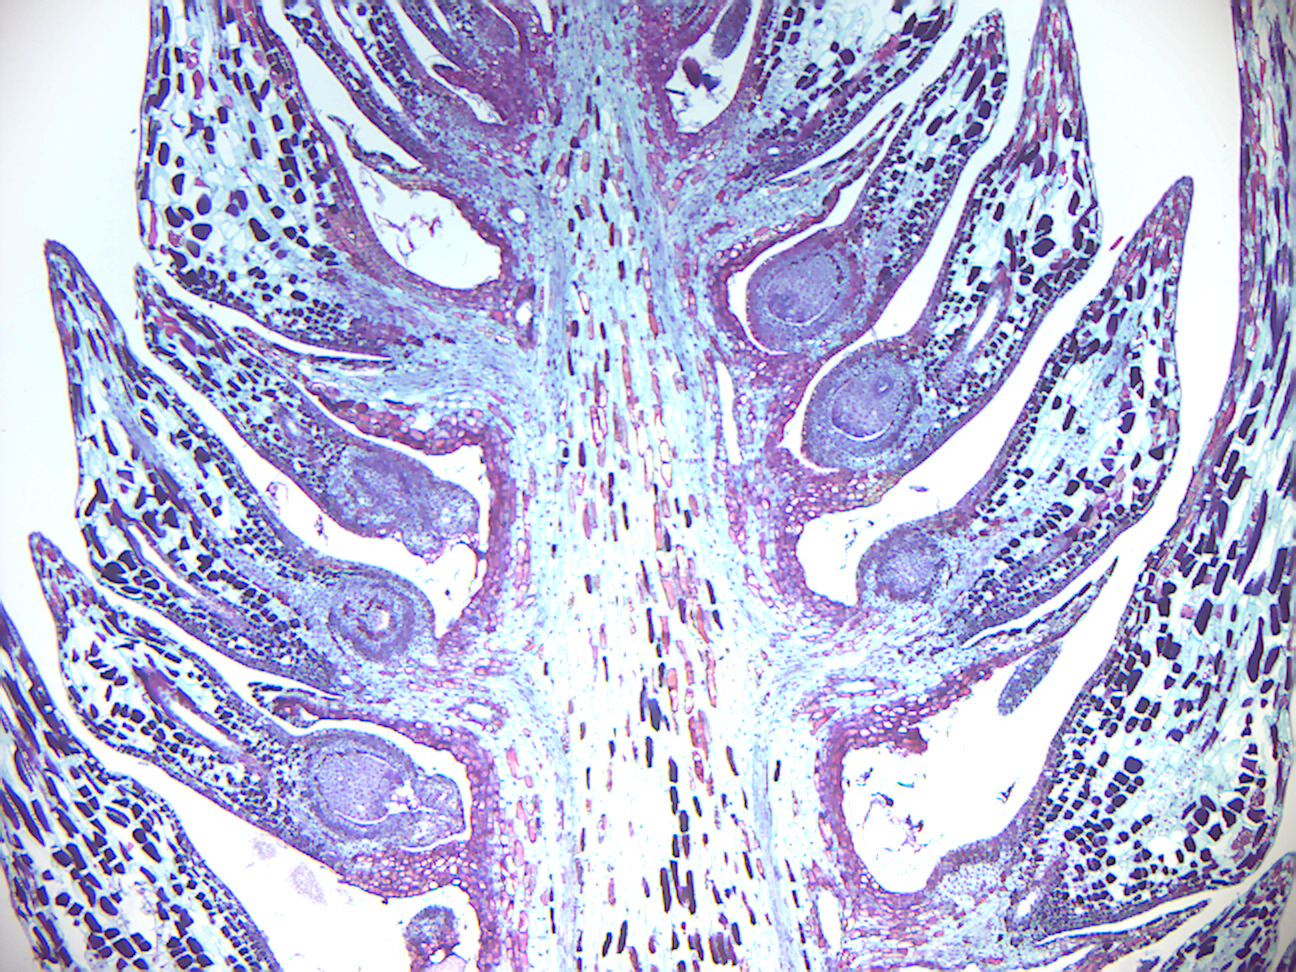
\includegraphics[width=0.7\linewidth]{./figures/gymnosperms/pine_ovulate}

}

\caption{Pine young ovulate cone.}\label{fig:ovulate}
\end{figure}

\begin{figure}

{\centering 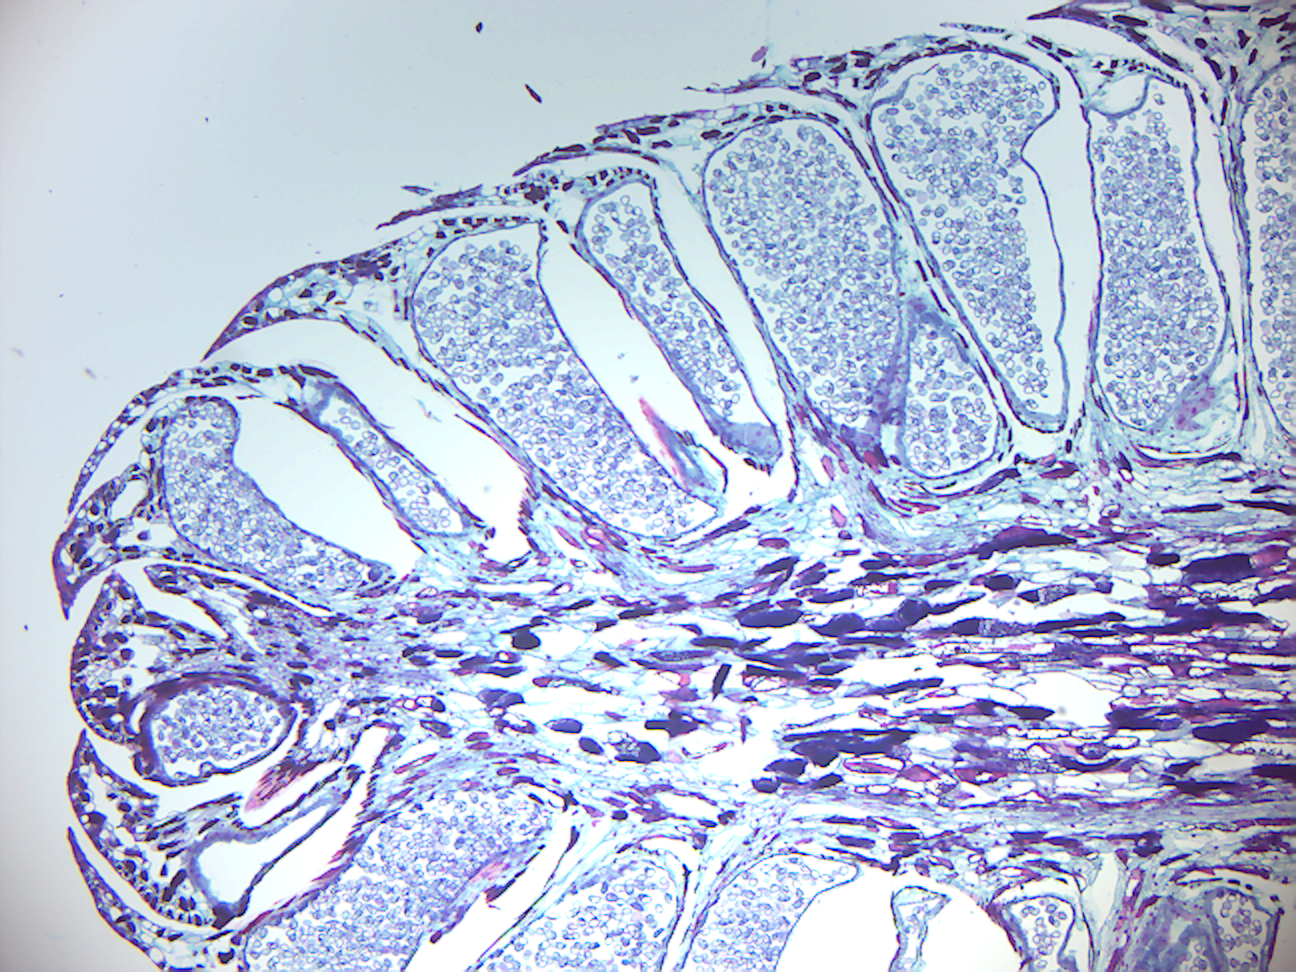
\includegraphics[width=0.7\linewidth]{./figures/gymnosperms/pine_staminate}

}

\caption{Pine staminate cone.}\label{fig:staminate}
\end{figure}

\begin{figure}

{\centering 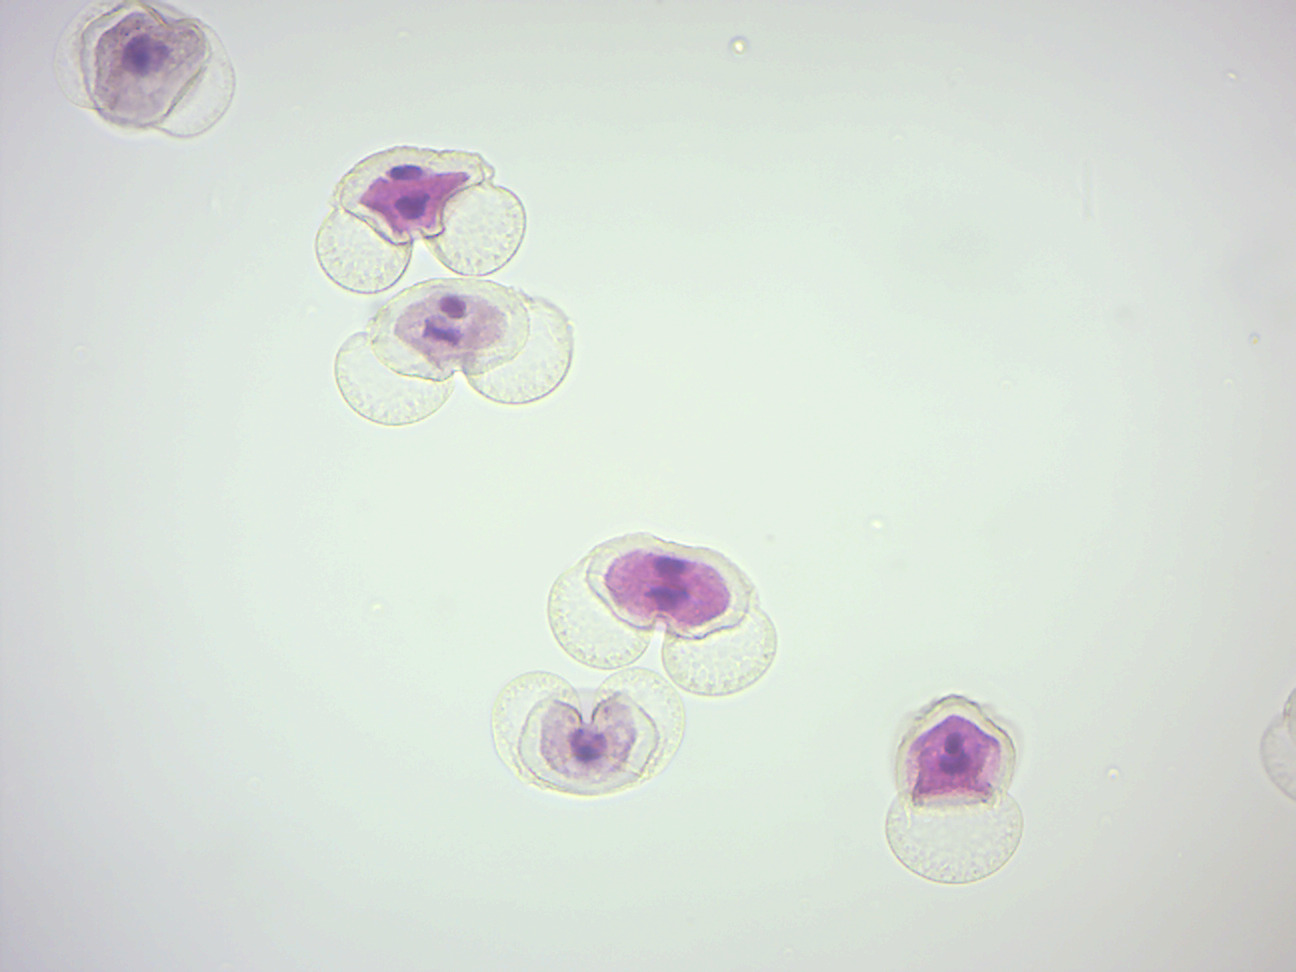
\includegraphics[width=0.7\linewidth]{./figures/gymnosperms/pine_pollen}

}

\caption{Pine pollen.}\label{fig:pollen}
\end{figure}

\begin{figure}

{\centering 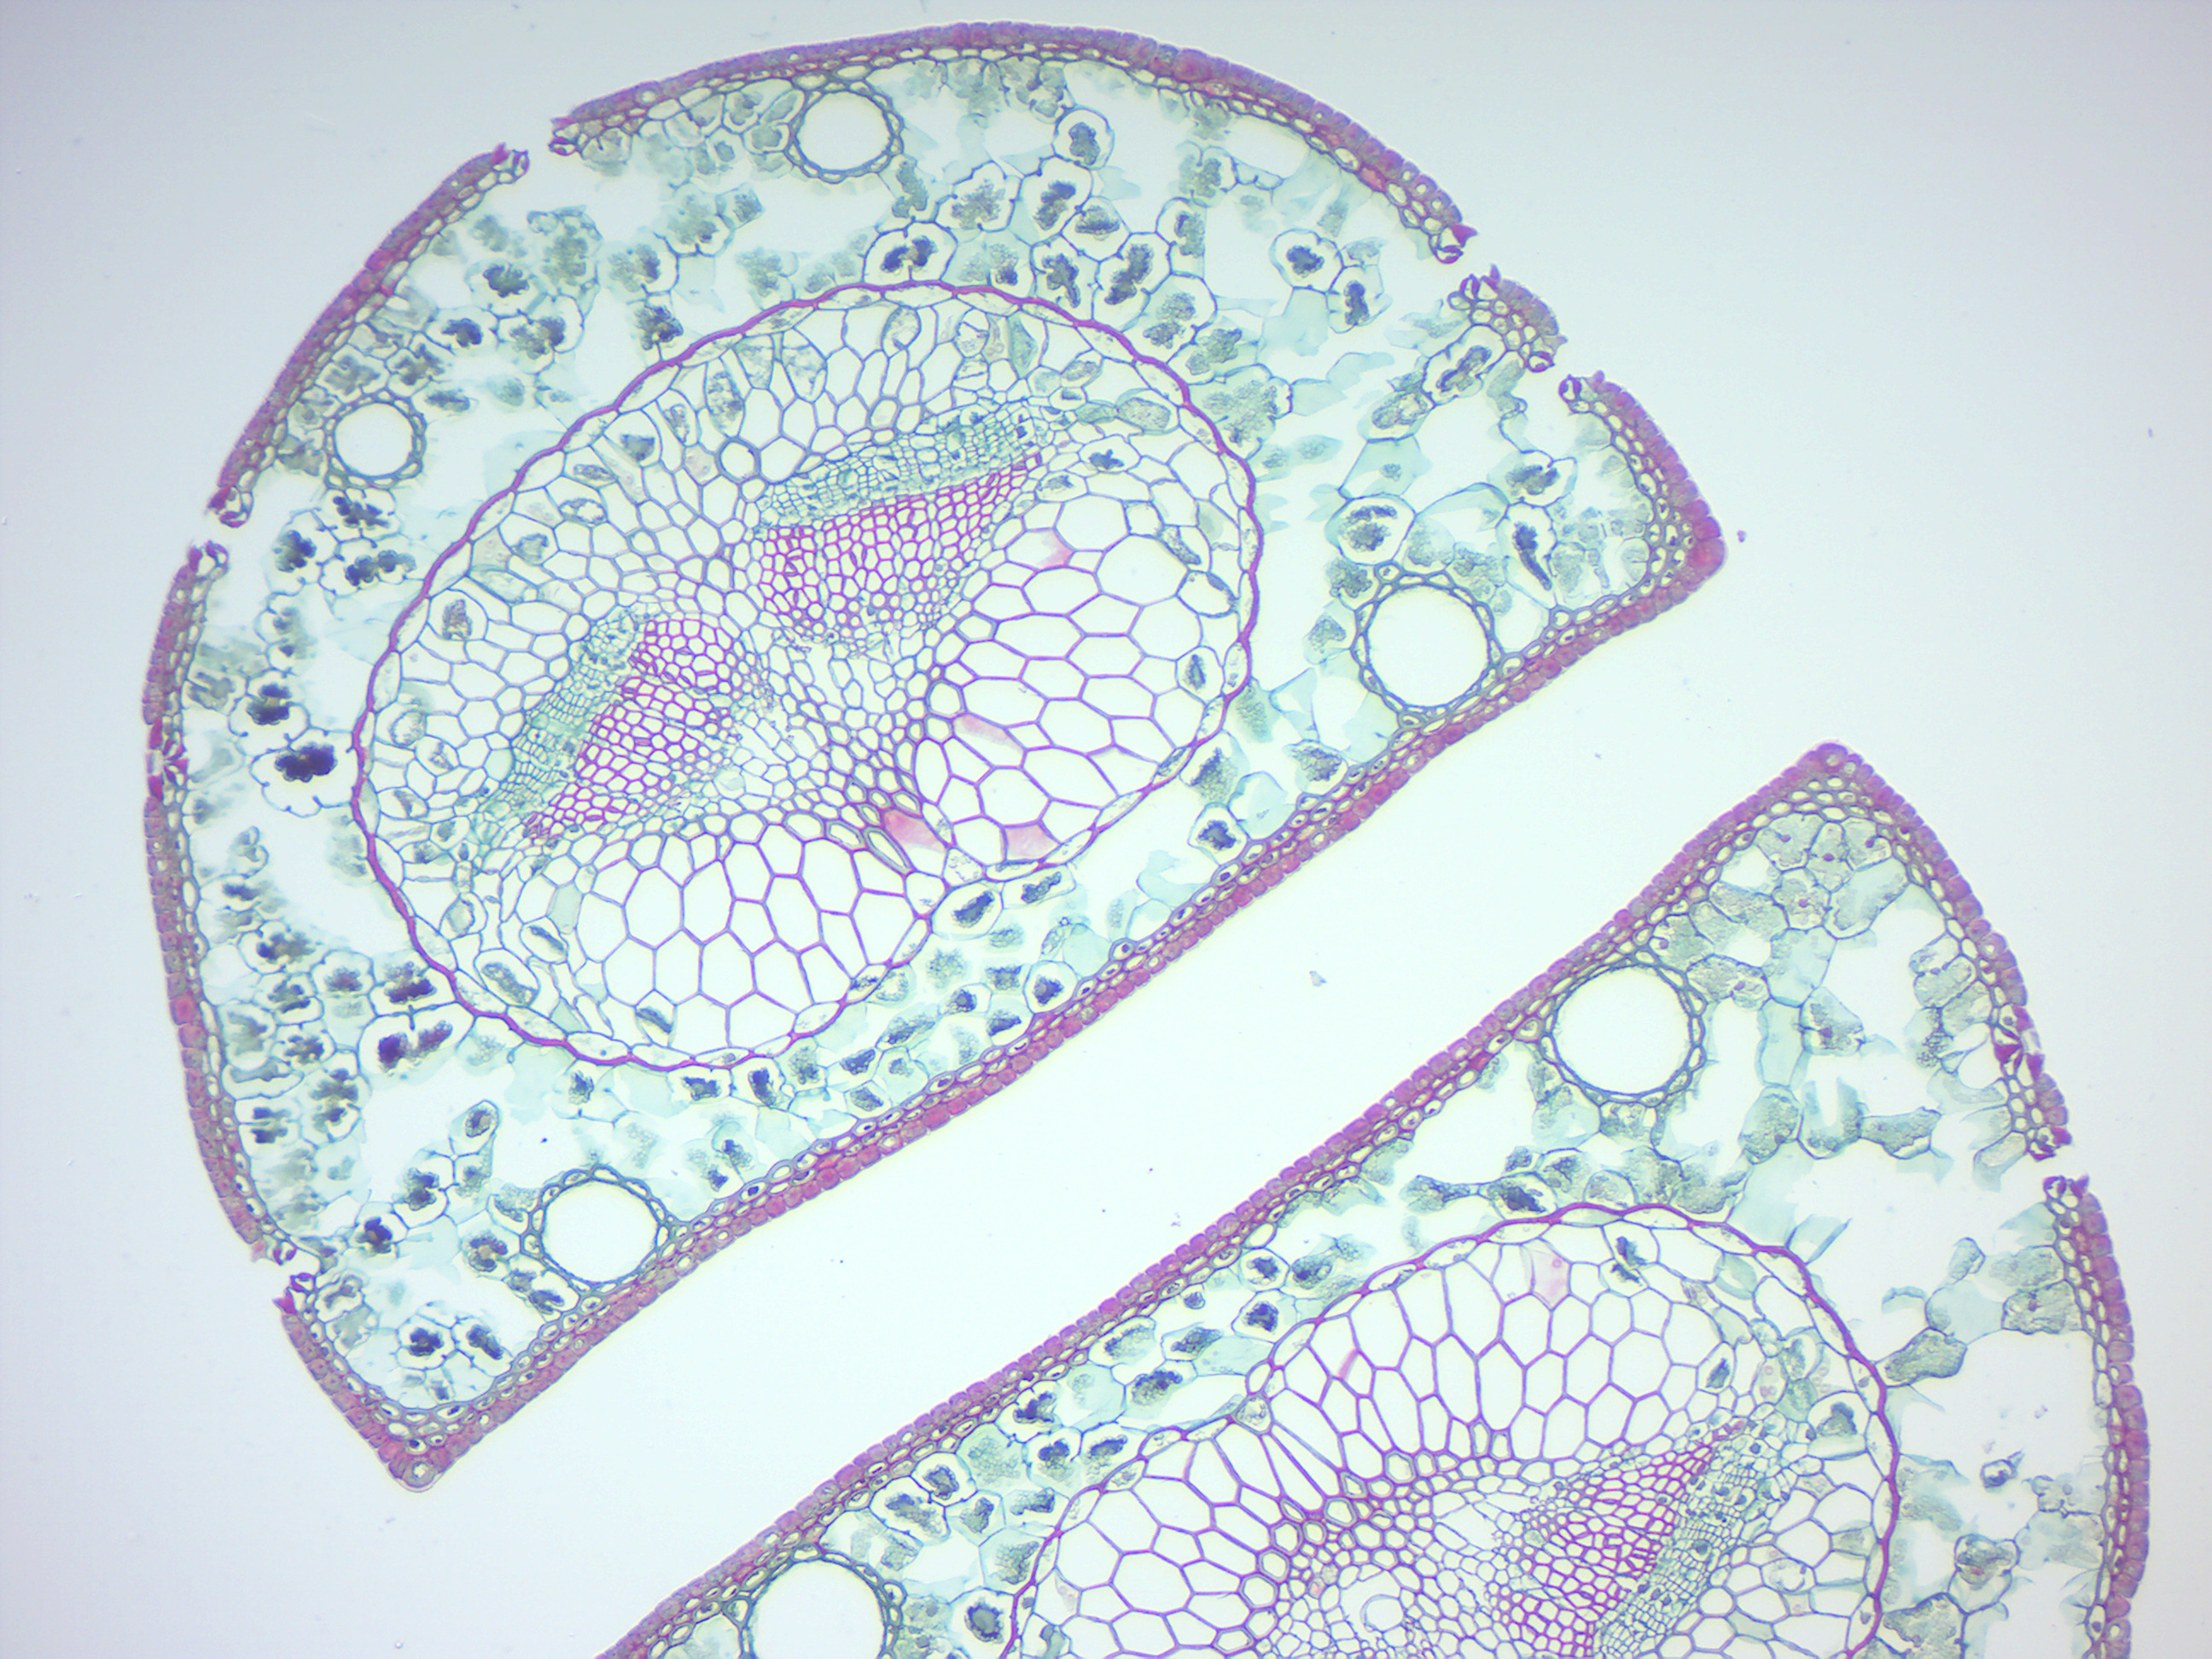
\includegraphics[width=0.7\linewidth]{./figures/gymnosperms/pine_needle}

}

\caption{Pine needle.}\label{fig:needle}
\end{figure}

\section{Angiosperms}\label{angiosperms}

The flowering plants, also known as angiosperms, Angiospermae or
Magnoliophyta, are the most diverse group of land plants, with 416
families, approximately 13,164 known genera and c. 295,383 known
species. Like gymnosperms, angiosperms are seed-producing plants.
However, they are distinguished from gymnosperms by characteristics
including flowers, endosperm within the seeds, and the production of
fruits that contain the seeds. Etymologically, angiosperm means a plant
that produces seeds within an enclosure; in other words, a fruiting
plant. The term comes from the Greek words angeion (``case'' or
``casing'') and sperma (``seed''). The ancestors of flowering plants
diverged from gymnosperms in the Triassic Period, 245 to 202 million
years ago (mya), and the first flowering plants are known from 160 mya.
They diversified extensively during the Lower Cretaceous, became
widespread by 120 mya, and replaced conifers as the dominant trees from
100 to 60 mya.

The characteristic feature of angiosperms is the flower. Flowers show
remarkable variation in form and elaboration, and provide the most
trustworthy external characteristics for establishing relationships
among angiosperm species. The function of the flower is to ensure
fertilization of the ovule and development of fruit containing seeds.
The floral apparatus may arise terminally on a shoot or from the axil of
a leaf (where the petiole attaches to the stem). Occasionally, as in
violets, a flower arises singly in the axil of an ordinary foliage-leaf.
More typically, the flower-bearing portion of the plant is sharply
distinguished from the foliage-bearing or vegetative portion, and forms
a more or less elaborate branch-system called an inflorescence.

\begin{figure}

{\centering 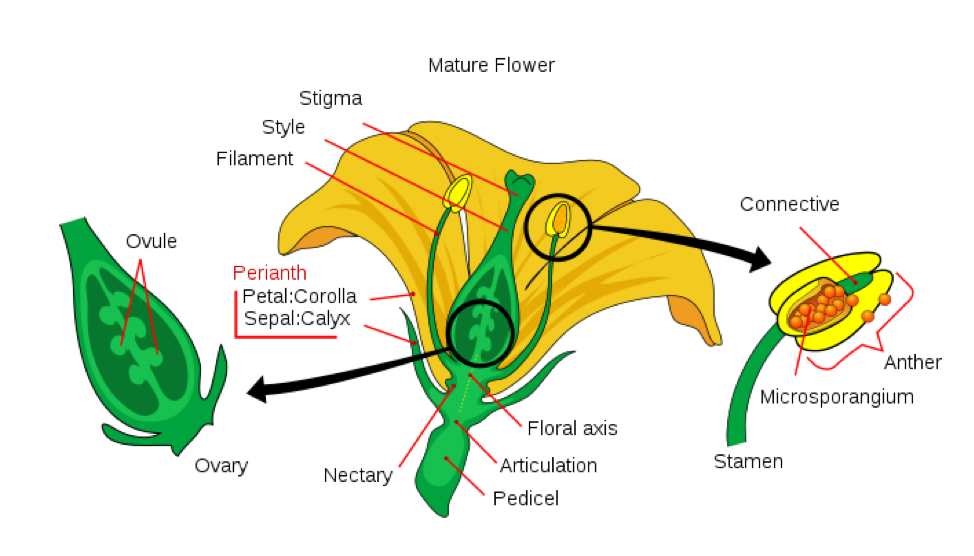
\includegraphics[width=0.7\linewidth]{./figures/gymnosperms/mature_flower}

}

\caption{\href{https://commons.wikimedia.org/wiki/File:Mature_flower_diagram.svg}{Anatomy
of the flower.}}\label{fig:flower}
\end{figure}

There are two kinds of reproductive cells produced by flowers.
Microspores, which will divide to become pollen grains, are the ``male''
cells and are borne in the stamens (or microsporophylls). The ``female''
cells called megaspores, which will divide to become the egg cell
(megagametogenesis), are contained in the ovule and enclosed in the
carpel (or megasporophyll).

The flower may consist only of these parts, as in willow, where each
flower comprises only a few stamens or two carpels. Usually, other
structures are present and serve to protect the sporophylls and to form
an envelope attractive to pollinators. The individual members of these
surrounding structures are known as sepals and petals (or tepals in
flowers such as \emph{Lilium} where sepals and petals are not distinguishable
from each other). The outer series (calyx of sepals) is usually green
and leaf-like, and functions to protect the rest of the flower,
especially the bud. The inner series (corolla of petals) is, in general,
white or brightly colored, and is more delicate in structure. It
functions to attract insect or bird pollinators. Attraction is effected
by color, scent, and nectar, which may be secreted in some part of the
flower. The characteristics that attract pollinators account for the
popularity of flowers and flowering plants among humans.

While the majority of flowers are perfect or hermaphrodite (having both
pollen and ovule producing parts in the same flower structure),
flowering plants have developed numerous morphological and physiological
mechanisms to reduce or prevent self-fertilization. Heteromorphic
flowers have short carpels and long stamens, or vice versa, so animal
pollinators cannot easily transfer pollen to the pistil (receptive part
of the carpel). Homomorphic flowers may employ a biochemical
(physiological) mechanism called self-incompatibility to discriminate
between self and non-self pollen grains. In other species, the male and
female parts are morphologically separated, developing on different
flowers.

\subsection{Sexual Reproduction}\label{sexual-reproduction}

Double fertilization refers to a process in which two sperm cells
fertilize cells in the ovary. This process begins when a pollen grain
adheres to the stigma of the pistil (female reproductive structure),
germinates, and grows a long pollen tube. While this pollen tube is
growing, a haploid generative cell travels down the tube behind the tube
nucleus. The generative cell divides by mitosis to produce two haploid
(n) sperm cells. As the pollen tube grows, it makes its way from the
stigma, down the style and into the ovary. Here the pollen tube reaches
the micropyle of the ovule and digests its way into one of the
synergids, releasing its contents (which include the sperm cells). The
synergid that the cells were released into degenerates and one sperm
makes its way to fertilize the egg cell, producing a diploid (2n)
zygote. The second sperm cell fuses with both central cell nuclei,
producing a triploid (3n) cell. As the zygote develops into an embryo,
the triploid cell develops into the endosperm, which serves as the
embryo's food supply. The ovary will now develop into a fruit and the
ovule will develop into a seed.

As the development of embryo and endosperm proceeds within the embryo
sac, the sac wall enlarges and combines with the nucellus (which is
likewise enlarging) and the integument to form the seed coat. The ovary
wall develops to form the fruit or pericarp, whose form is closely
associated with type of seed dispersal system.

Frequently, the influence of fertilization is felt beyond the ovary, and
other parts of the flower take part in the formation of the fruit, e.g.,
the floral receptacle in the apple, strawberry, and others.

The character of the seed coat bears a definite relation to that of the
fruit. They protect the embryo and aid in dissemination; they may also
directly promote germination. Among plants with indehiscent fruits, in
general, the fruit provides protection for the embryo and secures
dissemination. In this case, the seed coat is only slightly developed.
If the fruit is dehiscent and the seed is exposed, in general, the
seed-coat is well developed, and must discharge the functions otherwise
executed by the fruit.

Flowering plants generate gametes using meiosis. Meiosis takes place in the ovule (a structure within the
ovary that is located within the pistil at the center of the flower). A
diploid cell (megaspore mother cell) in the ovule undergoes meiosis
(involving two successive cell divisions) to produce four cells
(megaspores or female gametes) with haploid nuclei. One of these four
cells (megaspore) then undergoes three successive mitotic divisions to
produce an immature embryo sac (megagametocyte) with eight haploid
nuclei. Next, these nuclei are segregated into separate cells by
cytokinesis to producing 3 antipodal cells, 2 synergid cells and an egg
cell. Two polar nuclei are left in the central cell of the embryo sac.

Pollen is also produced by meiosis in the male anther (microsporangium).
During meiosis, a diploid microspore mother cell undergoes two
successive meiotic divisions to produce 4 haploid cells (microspores or
male gametes). Each of these microspores, after further mitoses, becomes
a pollen grain (microgametophyte) containing two haploid generative
(sperm) cells and a tube nucleus. When a pollen grain makes contact with
the female stigma, the pollen grain forms a pollen tube that grows down
the style into the ovary. In the act of fertilization, a male sperm
nucleus fuses with the female egg nucleus to form a diploid zygote that
can then develop into an embryo within the newly forming seed. Upon
germination of the seed, a new plant can grow and mature.

\begin{figure}

{\centering 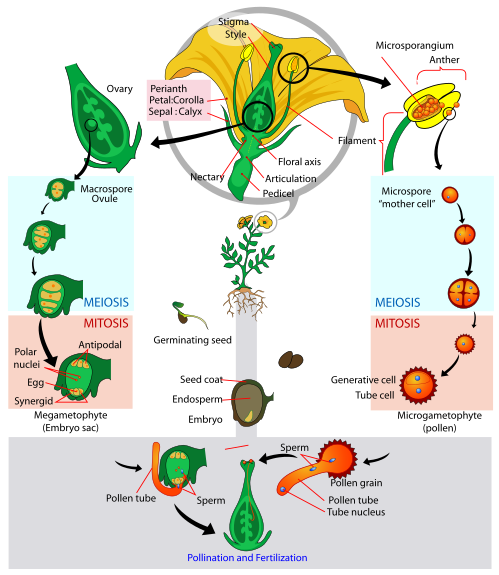
\includegraphics[width=0.7\linewidth]{./figures/gymnosperms/angiosperm_life_cycle}

}

\caption{\href{https://commons.wikimedia.org/wiki/File:Angiosperm_life_cycle_diagram-en.svg}{Life
cycle of angiosperms.}}\label{fig:angiosperm}
\end{figure}

\section{View Prepared Slides of
Angiosperms}\label{view-prepared-slides-of-angiosperms}

\begin{enumerate}
\def\labelenumi{\arabic{enumi}.}
\tightlist
\item
  Lily anther (Figure \ref{fig:lilianther})

  \begin{itemize}
  \tightlist
  \item
    Identify: anther, microsporangium, pollen grains with tube and
    generative nuclei. The structure in the middle of the slide is the
    Lily ovary. The anthers are around the ovary.
  \end{itemize}
\item
  Lily anther with mature pollen (Figure \ref{fig:lilipollen})

  \begin{itemize}
  \tightlist
  \item
    Identify: pollen grain, tube cell with nucleus, generative cell with
    nucleus
  \end{itemize}
\item
  Lily pollen tubes (Figure \ref{fig:lilitubes})

  \begin{itemize}
  \tightlist
  \item
    Identify: sigma tissue, pollen tubes
  \end{itemize}
\item
  Lily ovary (Figure \ref{fig:liliovary})

  \begin{itemize}
  \tightlist
  \item
    Identify: ovary, ovules, female gametophytes (embryo sac). If this
    slides is not available, you can observe the lily ovary in the
    ``Lily anther x.s.'' slide.
  \end{itemize}
\item
  \emph{Tilia} 2 year old stem (Figure \ref{fig:tilia})
\item
  \emph{Capsella} seeds (Figure \ref{fig:capsella})

  \begin{itemize}
  \tightlist
  \item
    Identify: embryo, cotyledons, root tip, shoot tip
  \end{itemize}
\end{enumerate}

\begin{figure}

{\centering 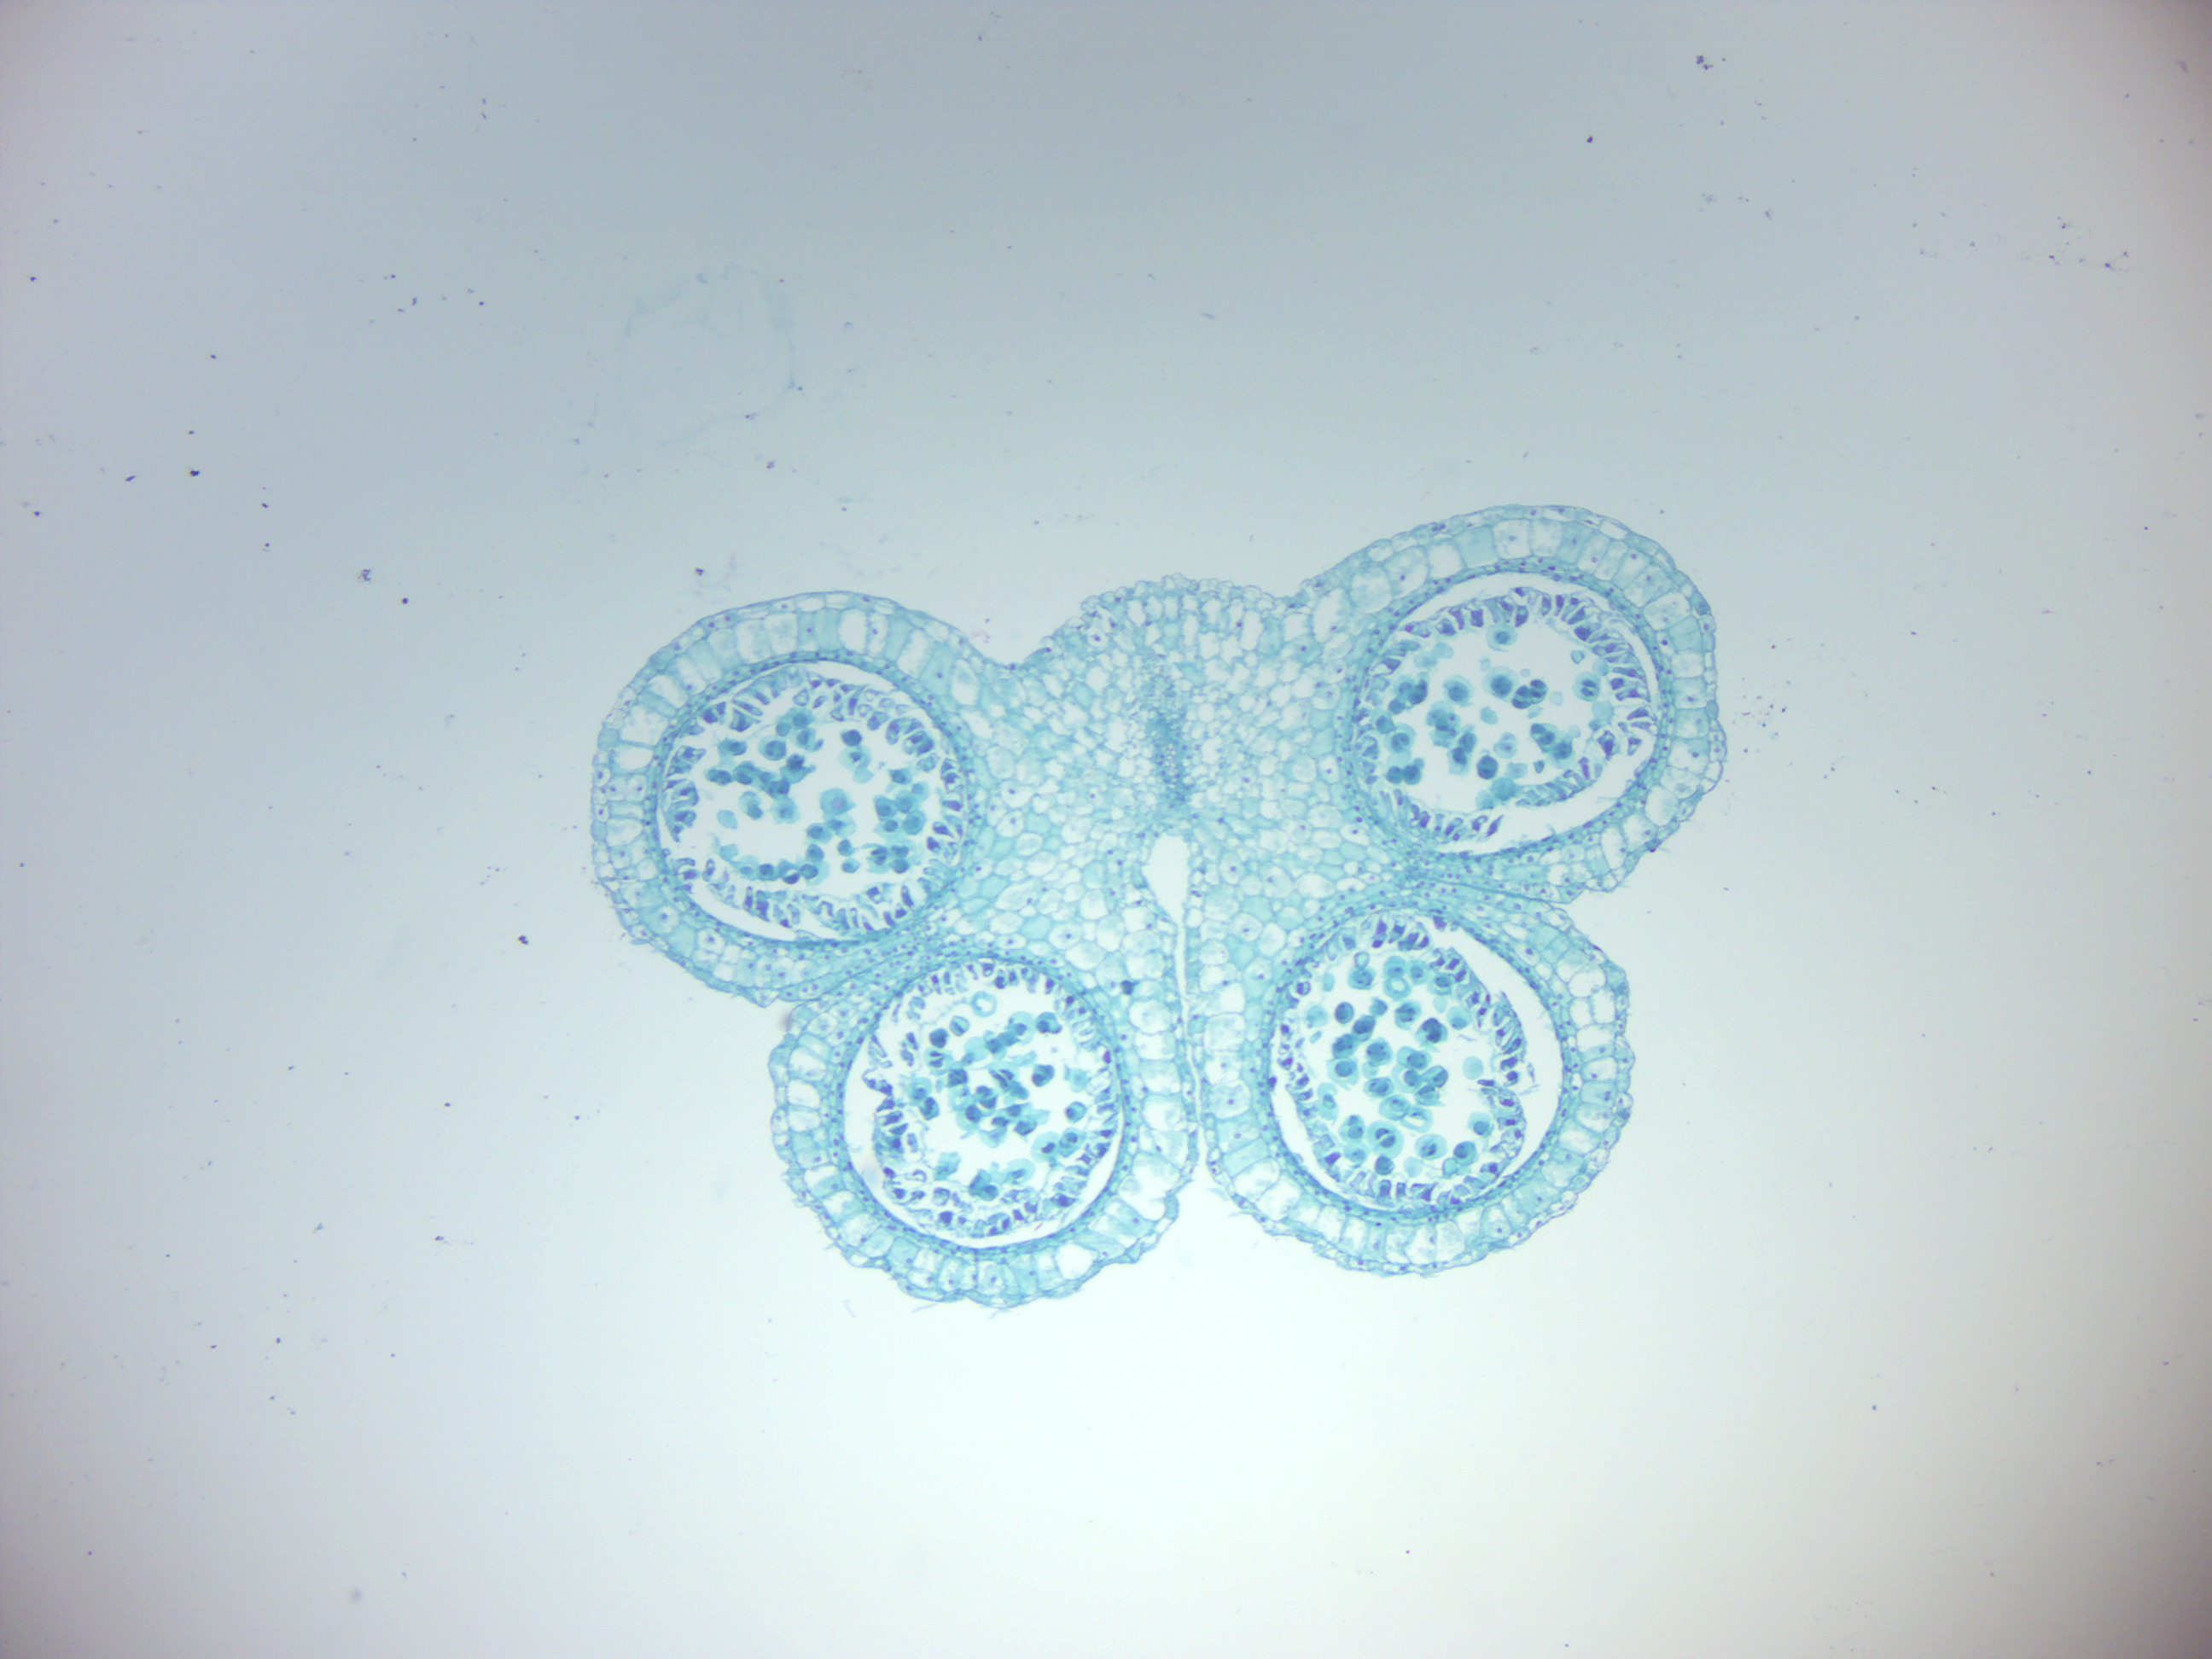
\includegraphics[width=0.7\linewidth]{./figures/gymnosperms/lily_anther}

}

\caption{Lily anther.}\label{fig:lilianther}
\end{figure}

\begin{figure}

{\centering 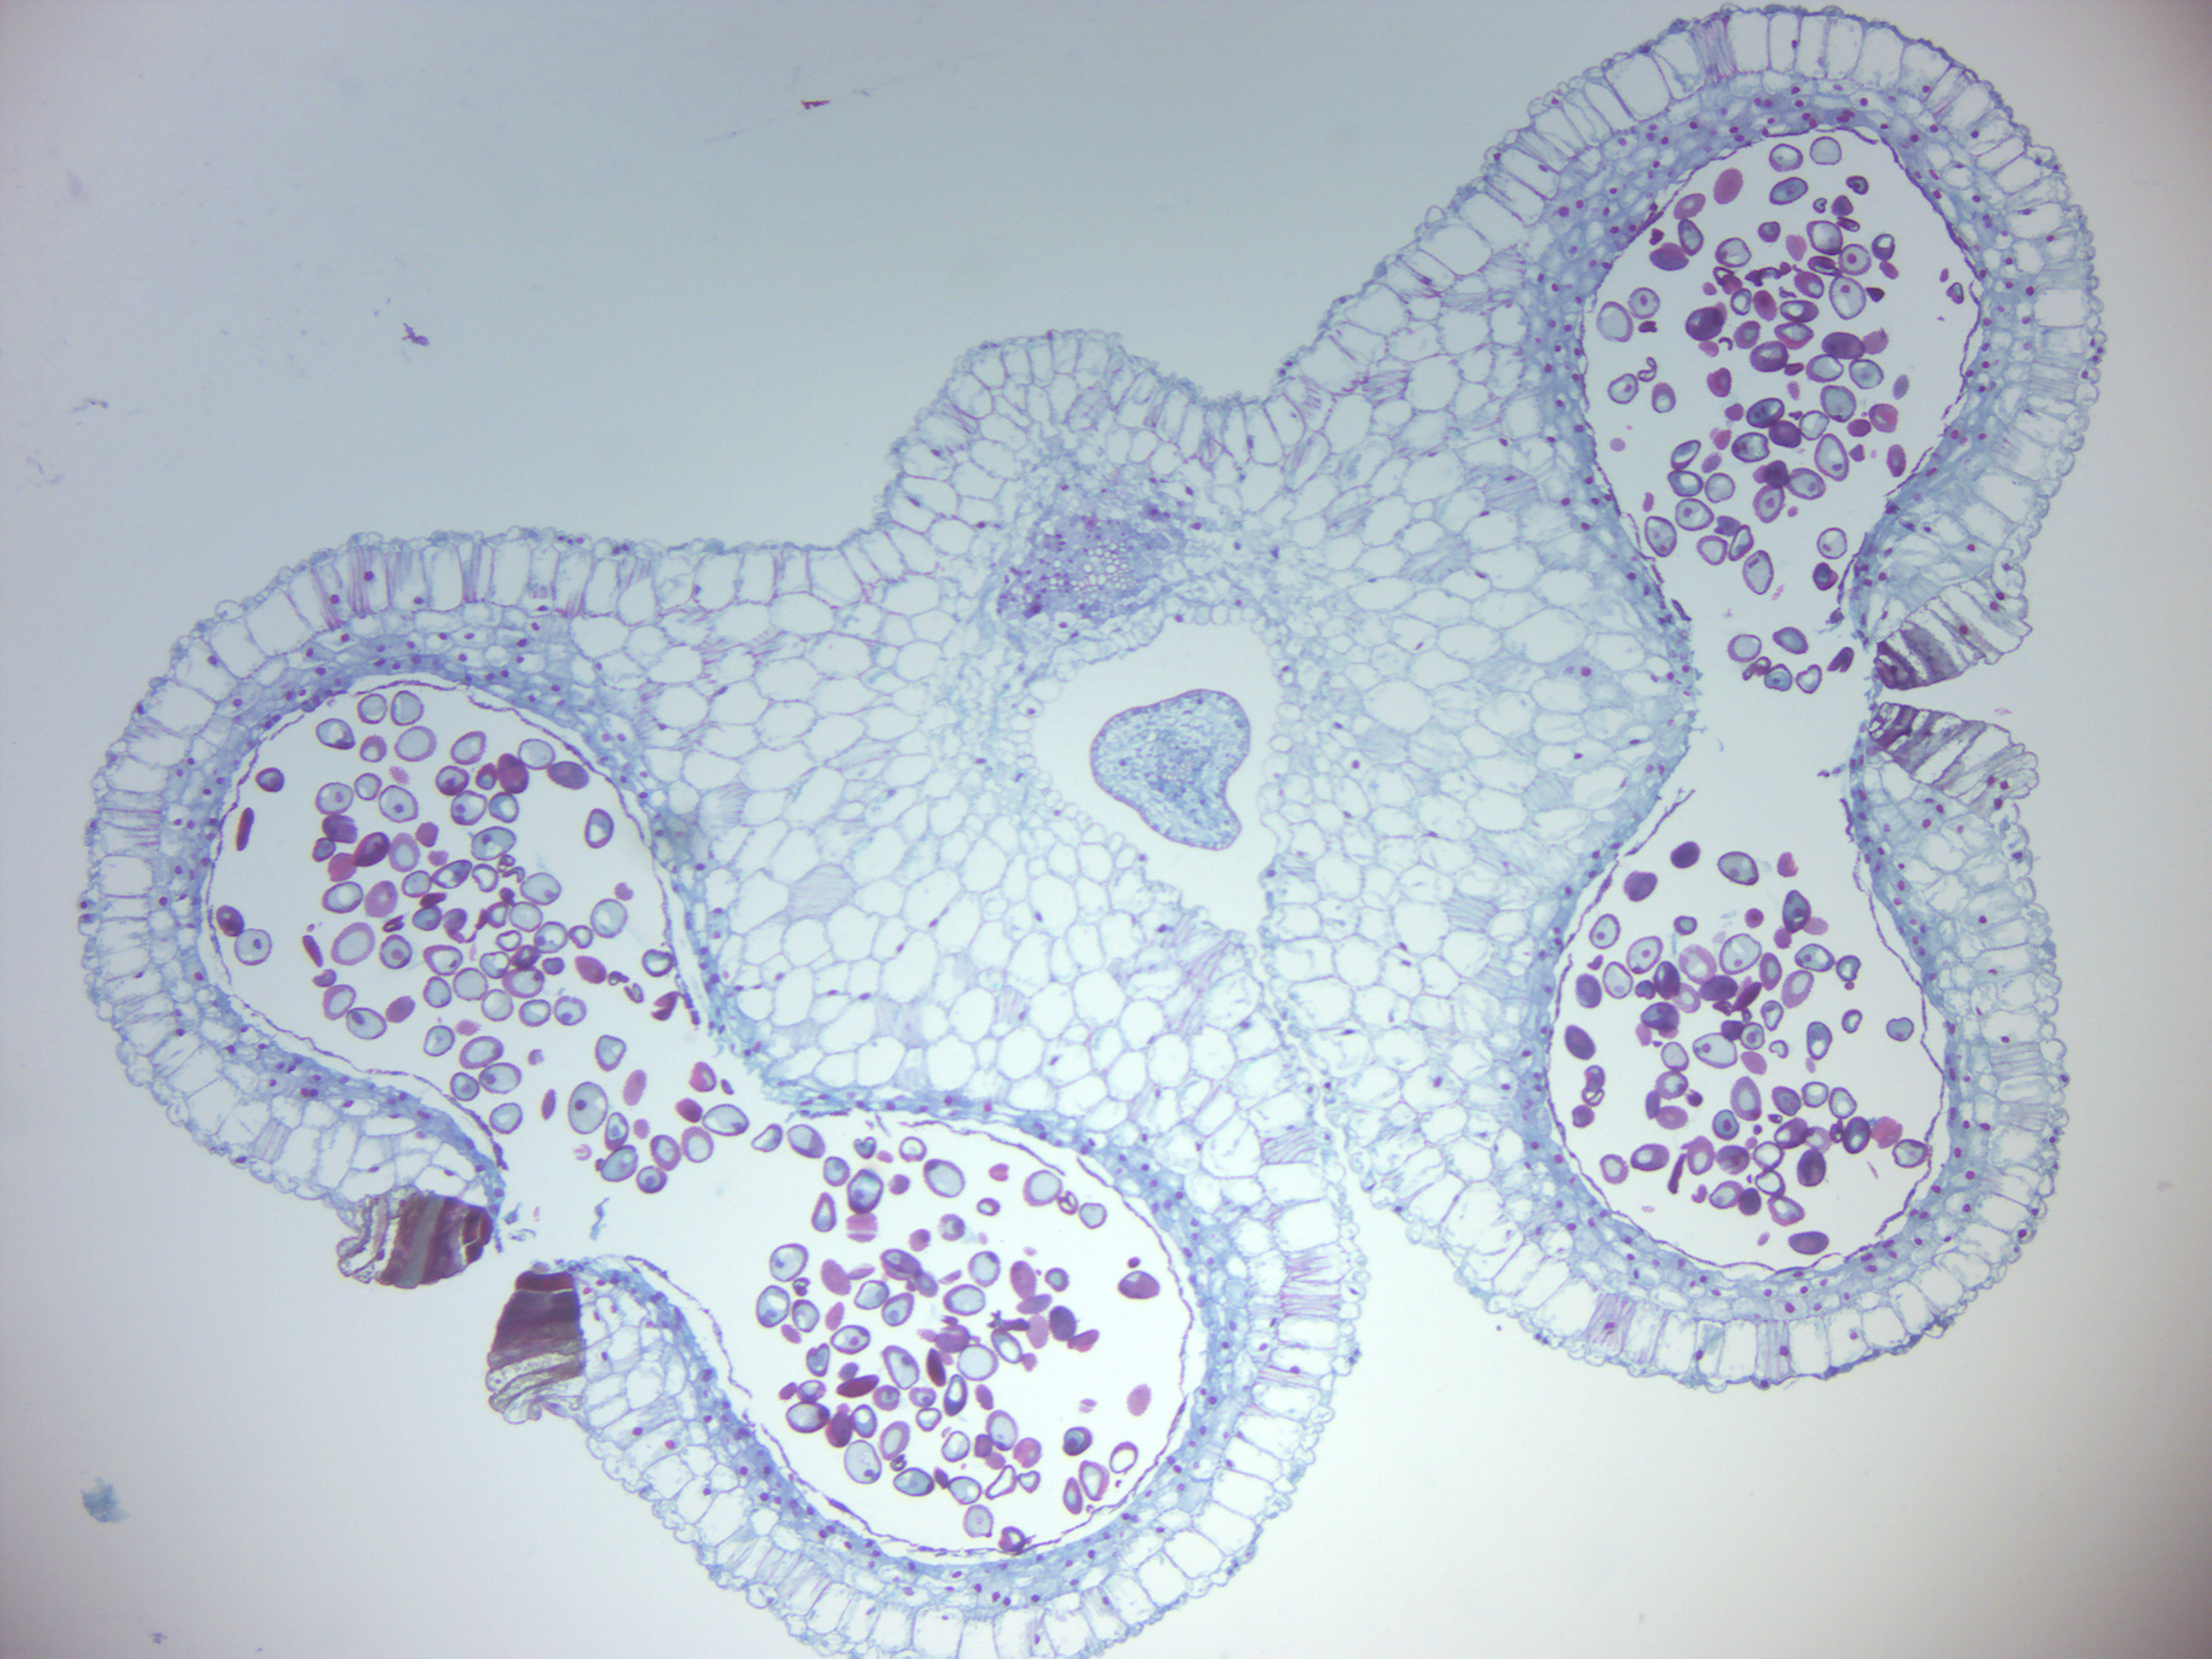
\includegraphics[width=0.7\linewidth]{./figures/gymnosperms/lily_pollen}

}

\caption{Lily anther with mature pollen.}\label{fig:lilipollen}
\end{figure}

\begin{figure}

{\centering 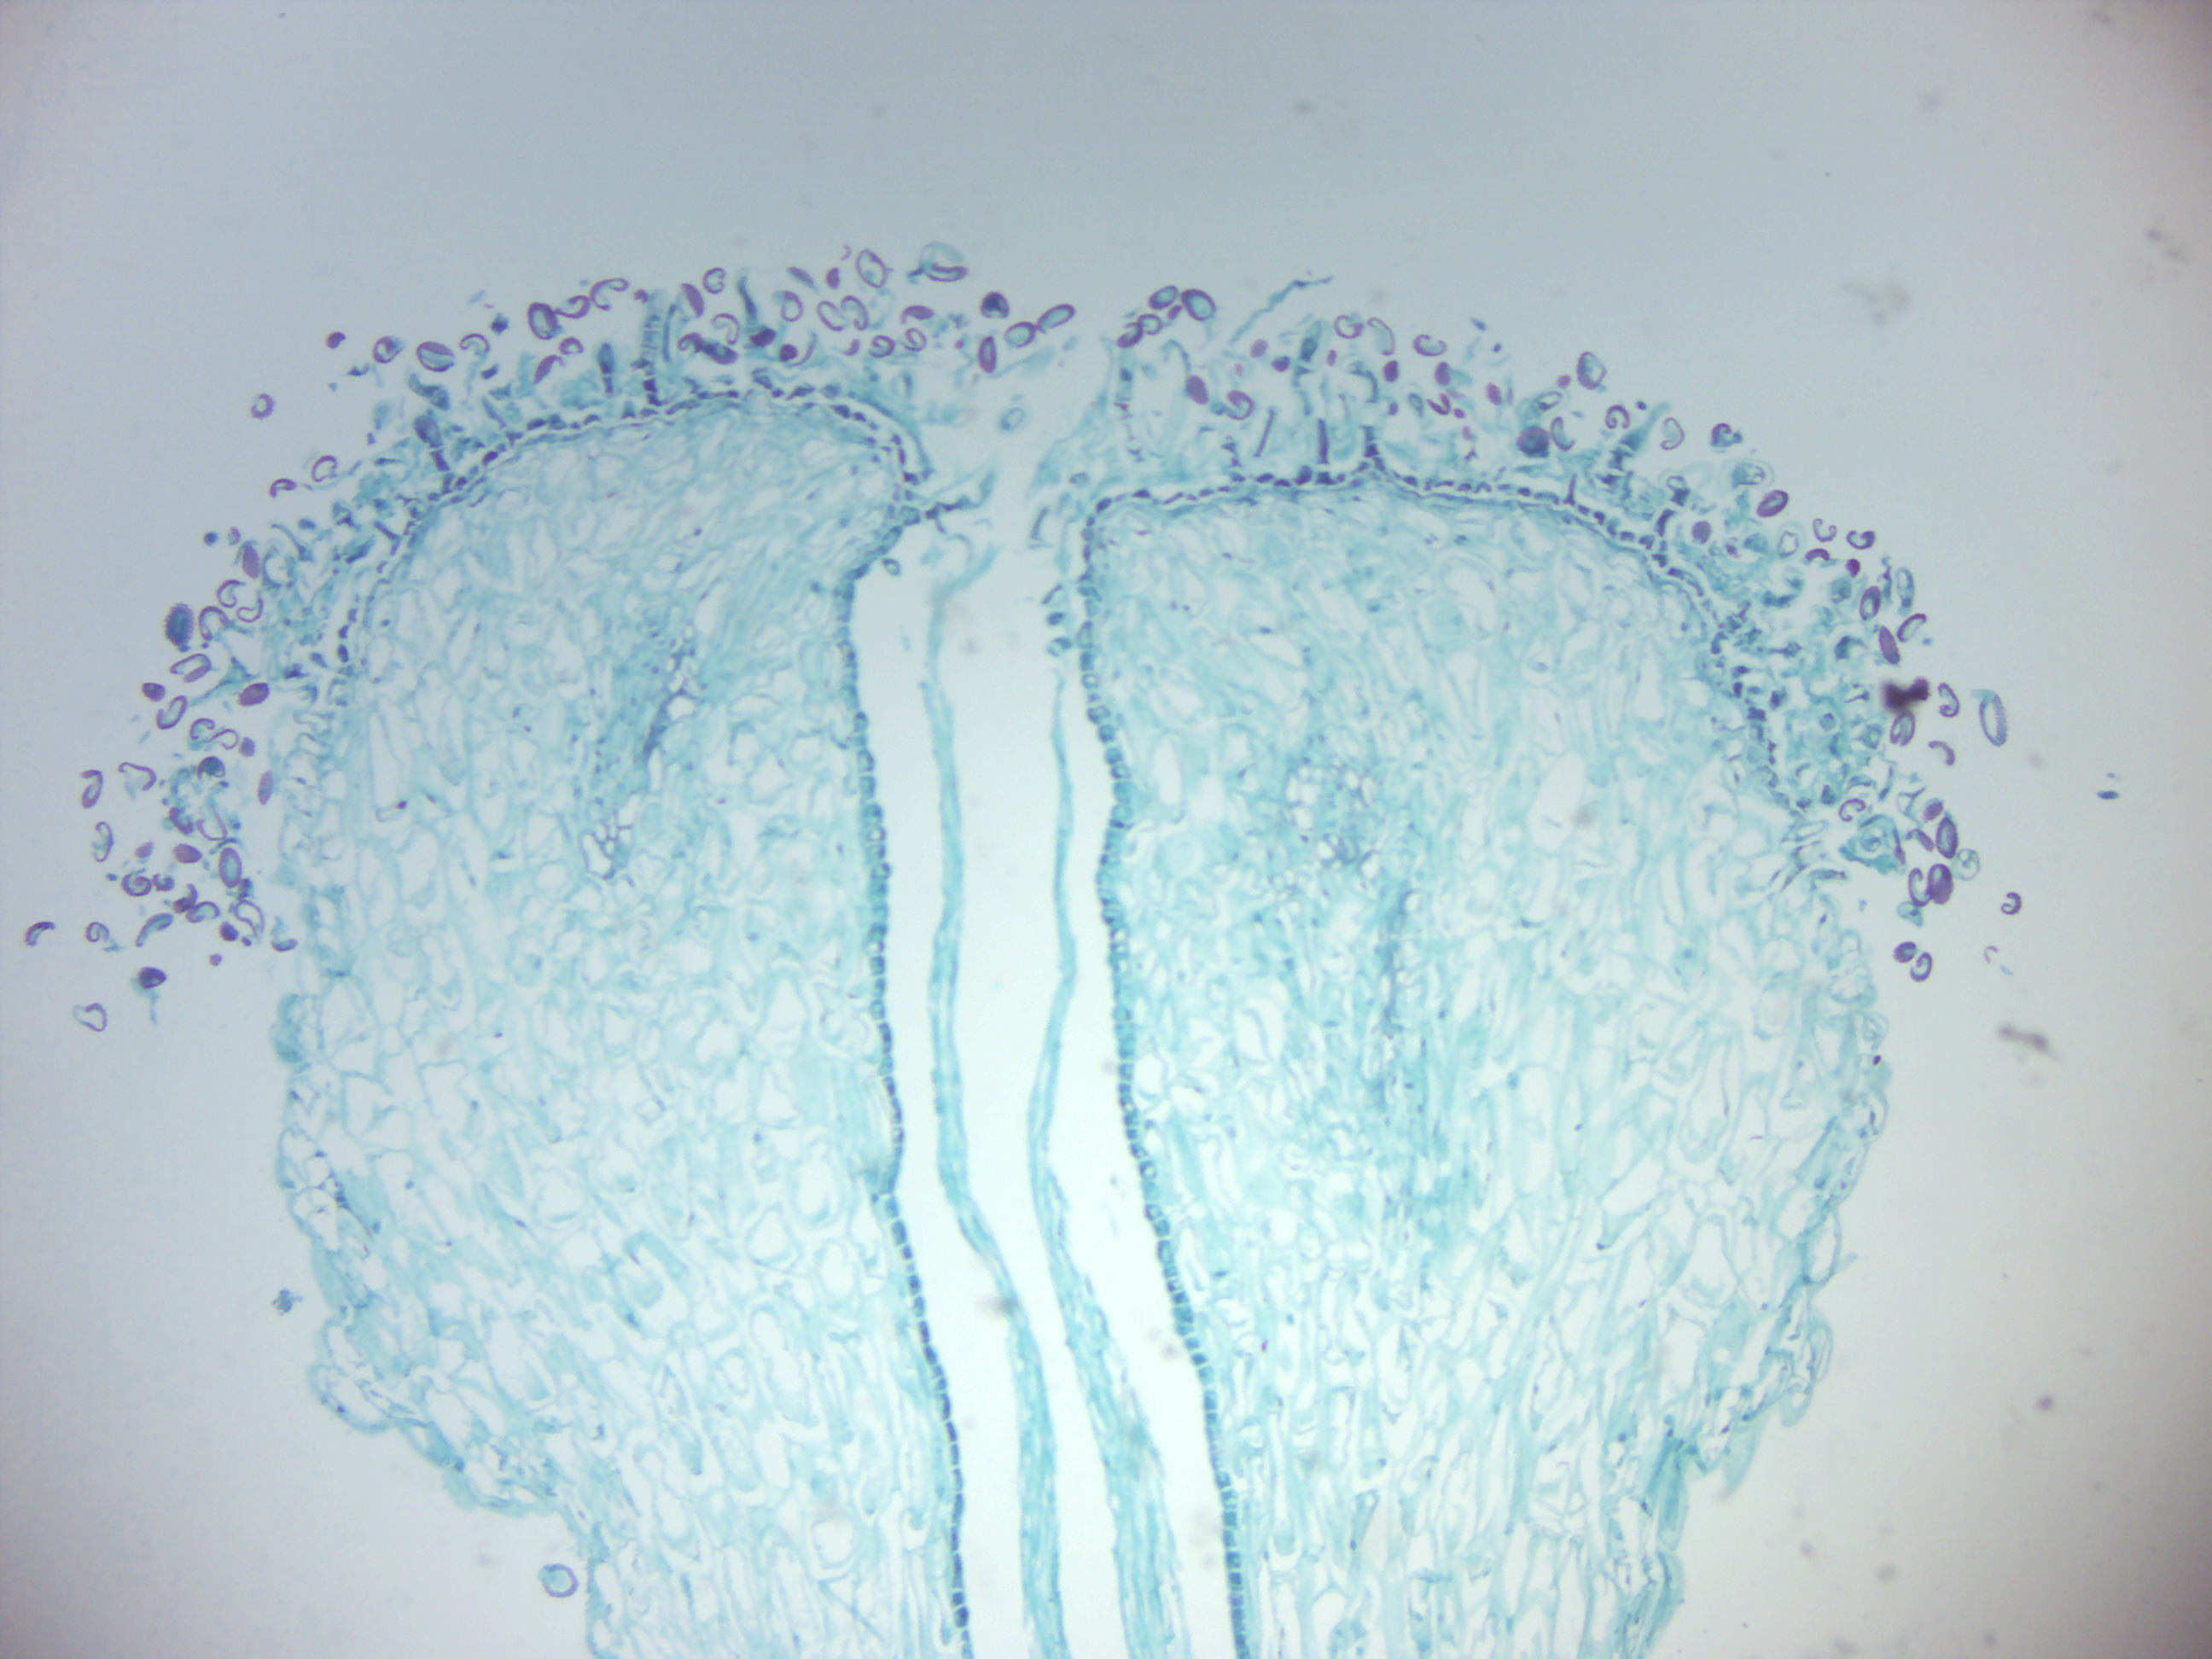
\includegraphics[width=0.7\linewidth]{./figures/gymnosperms/lily_tubes}

}

\caption{Lily pollen tubes.}\label{fig:lilitubes}
\end{figure}

\begin{figure}

{\centering 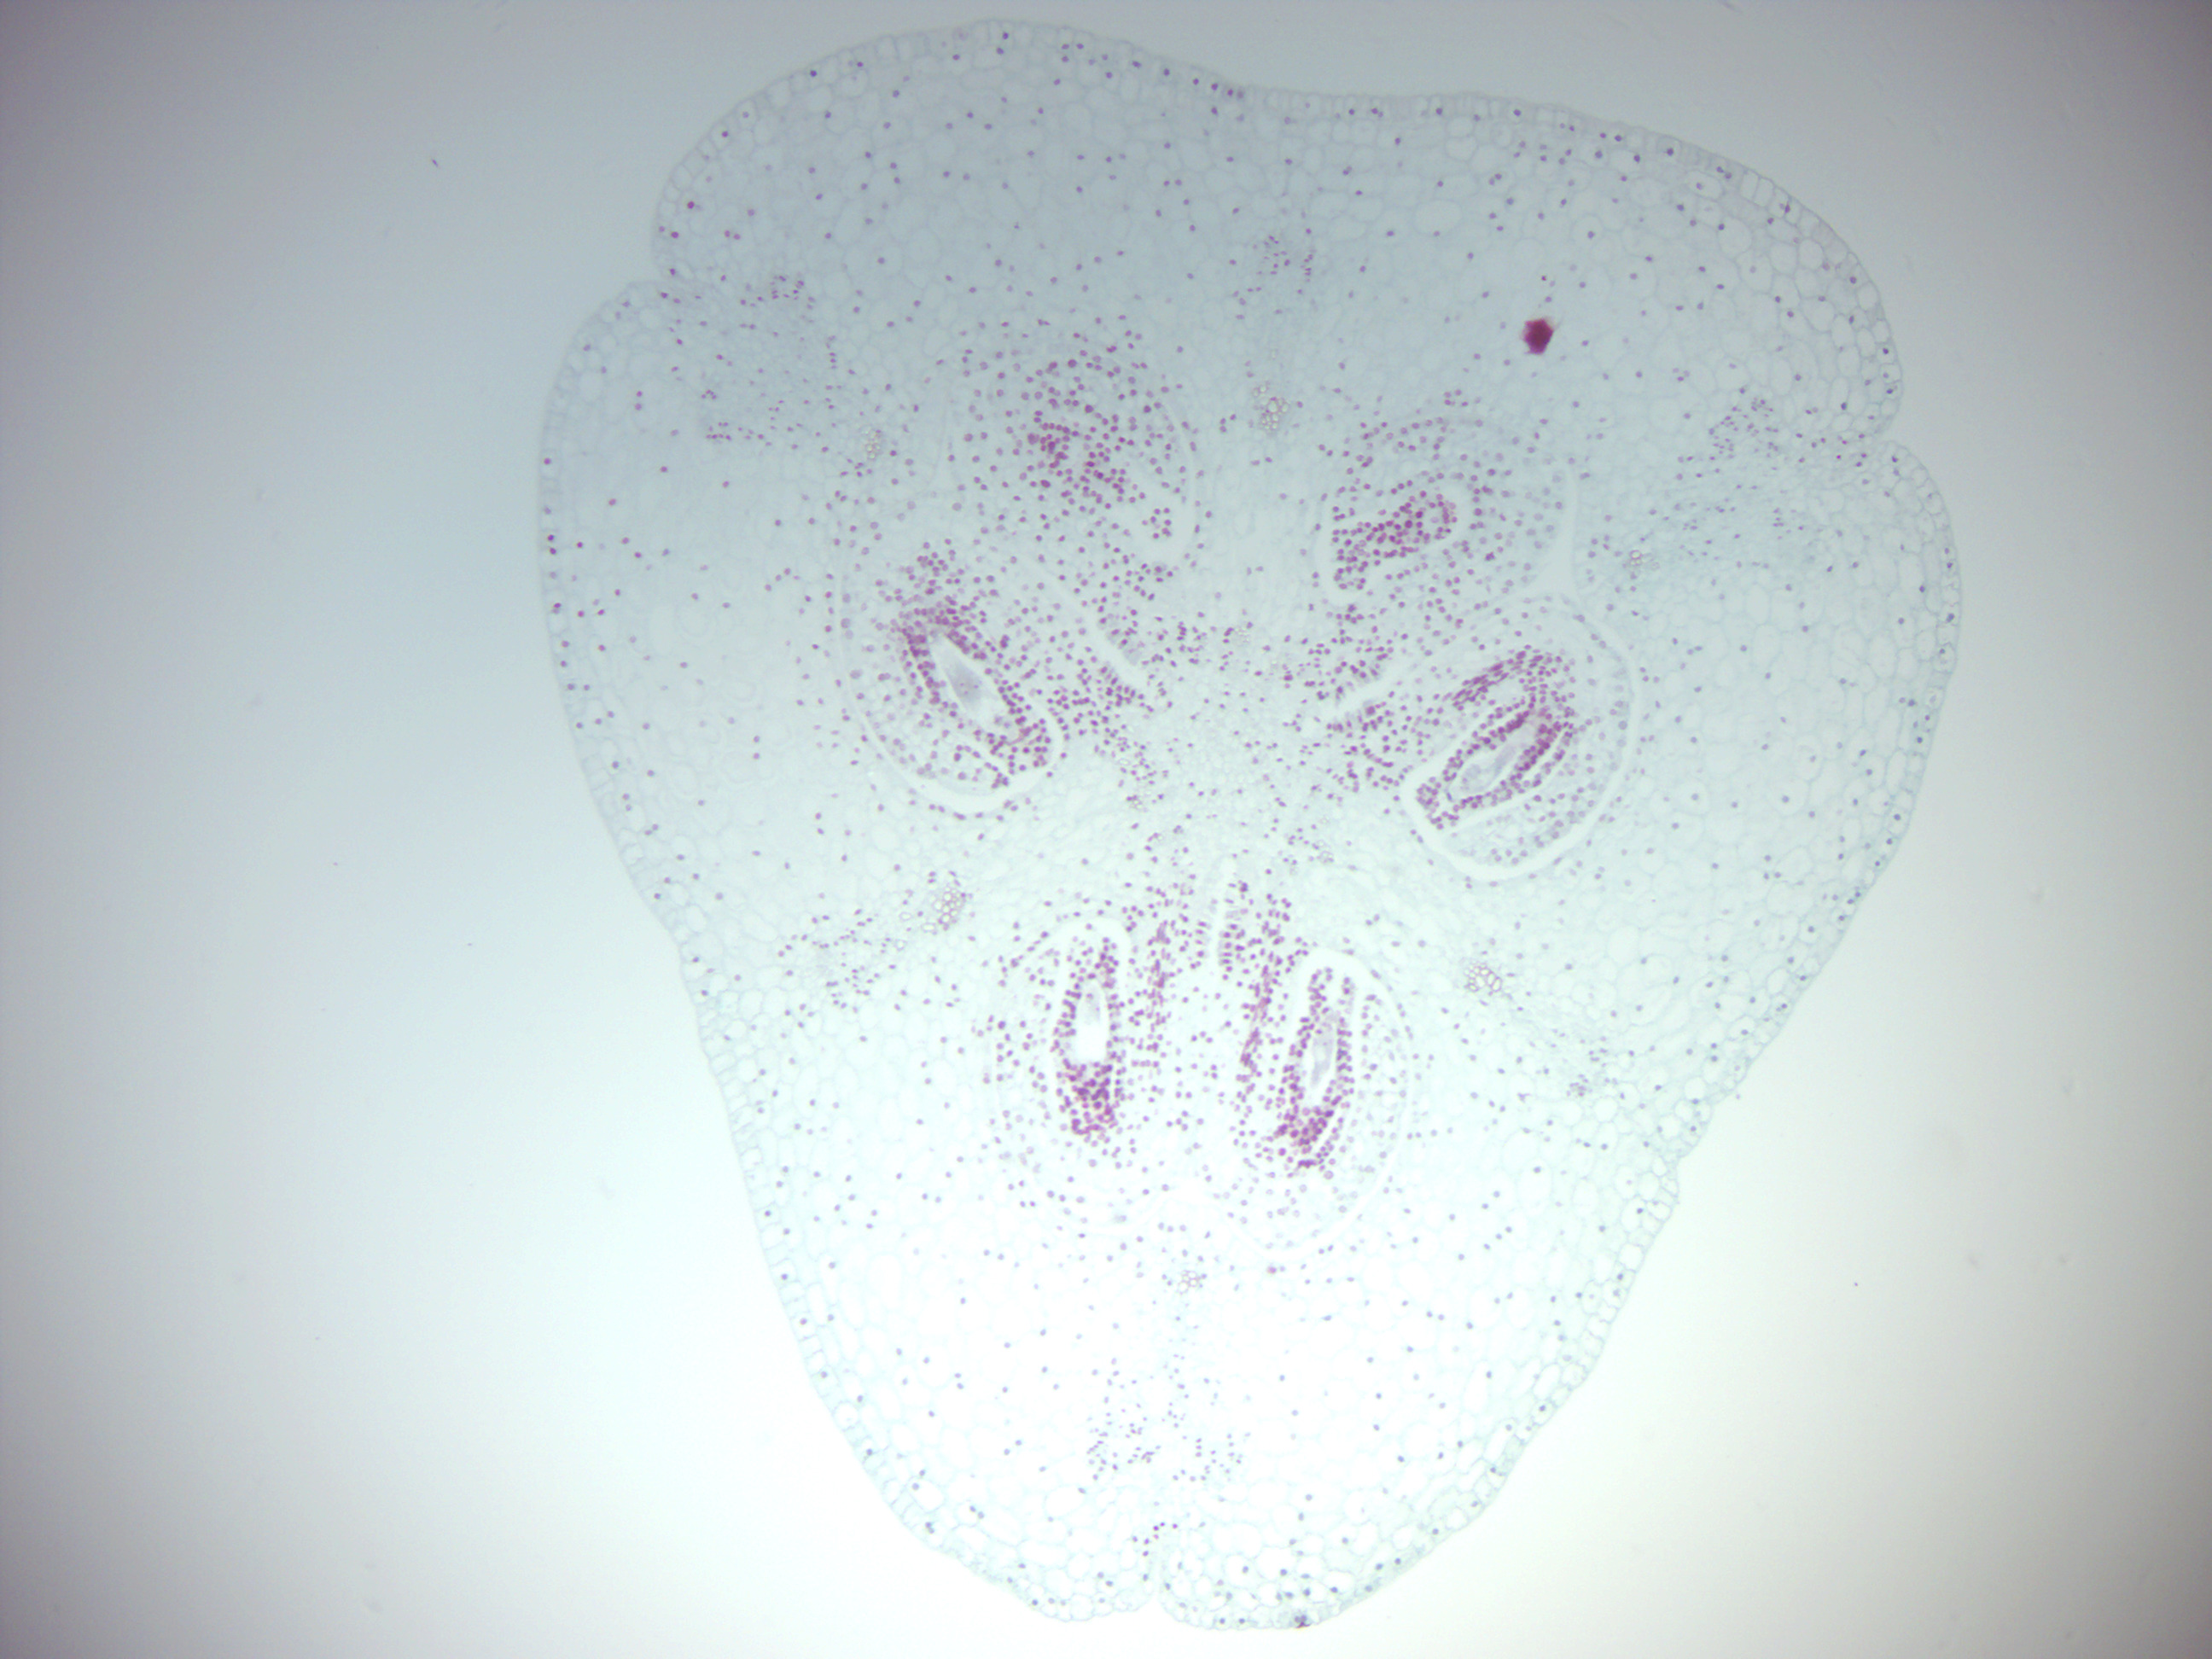
\includegraphics[width=0.7\linewidth]{./figures/gymnosperms/lily_ovary}

}

\caption{Lily ovary.}\label{fig:liliovary}
\end{figure}

\begin{figure}

{\centering 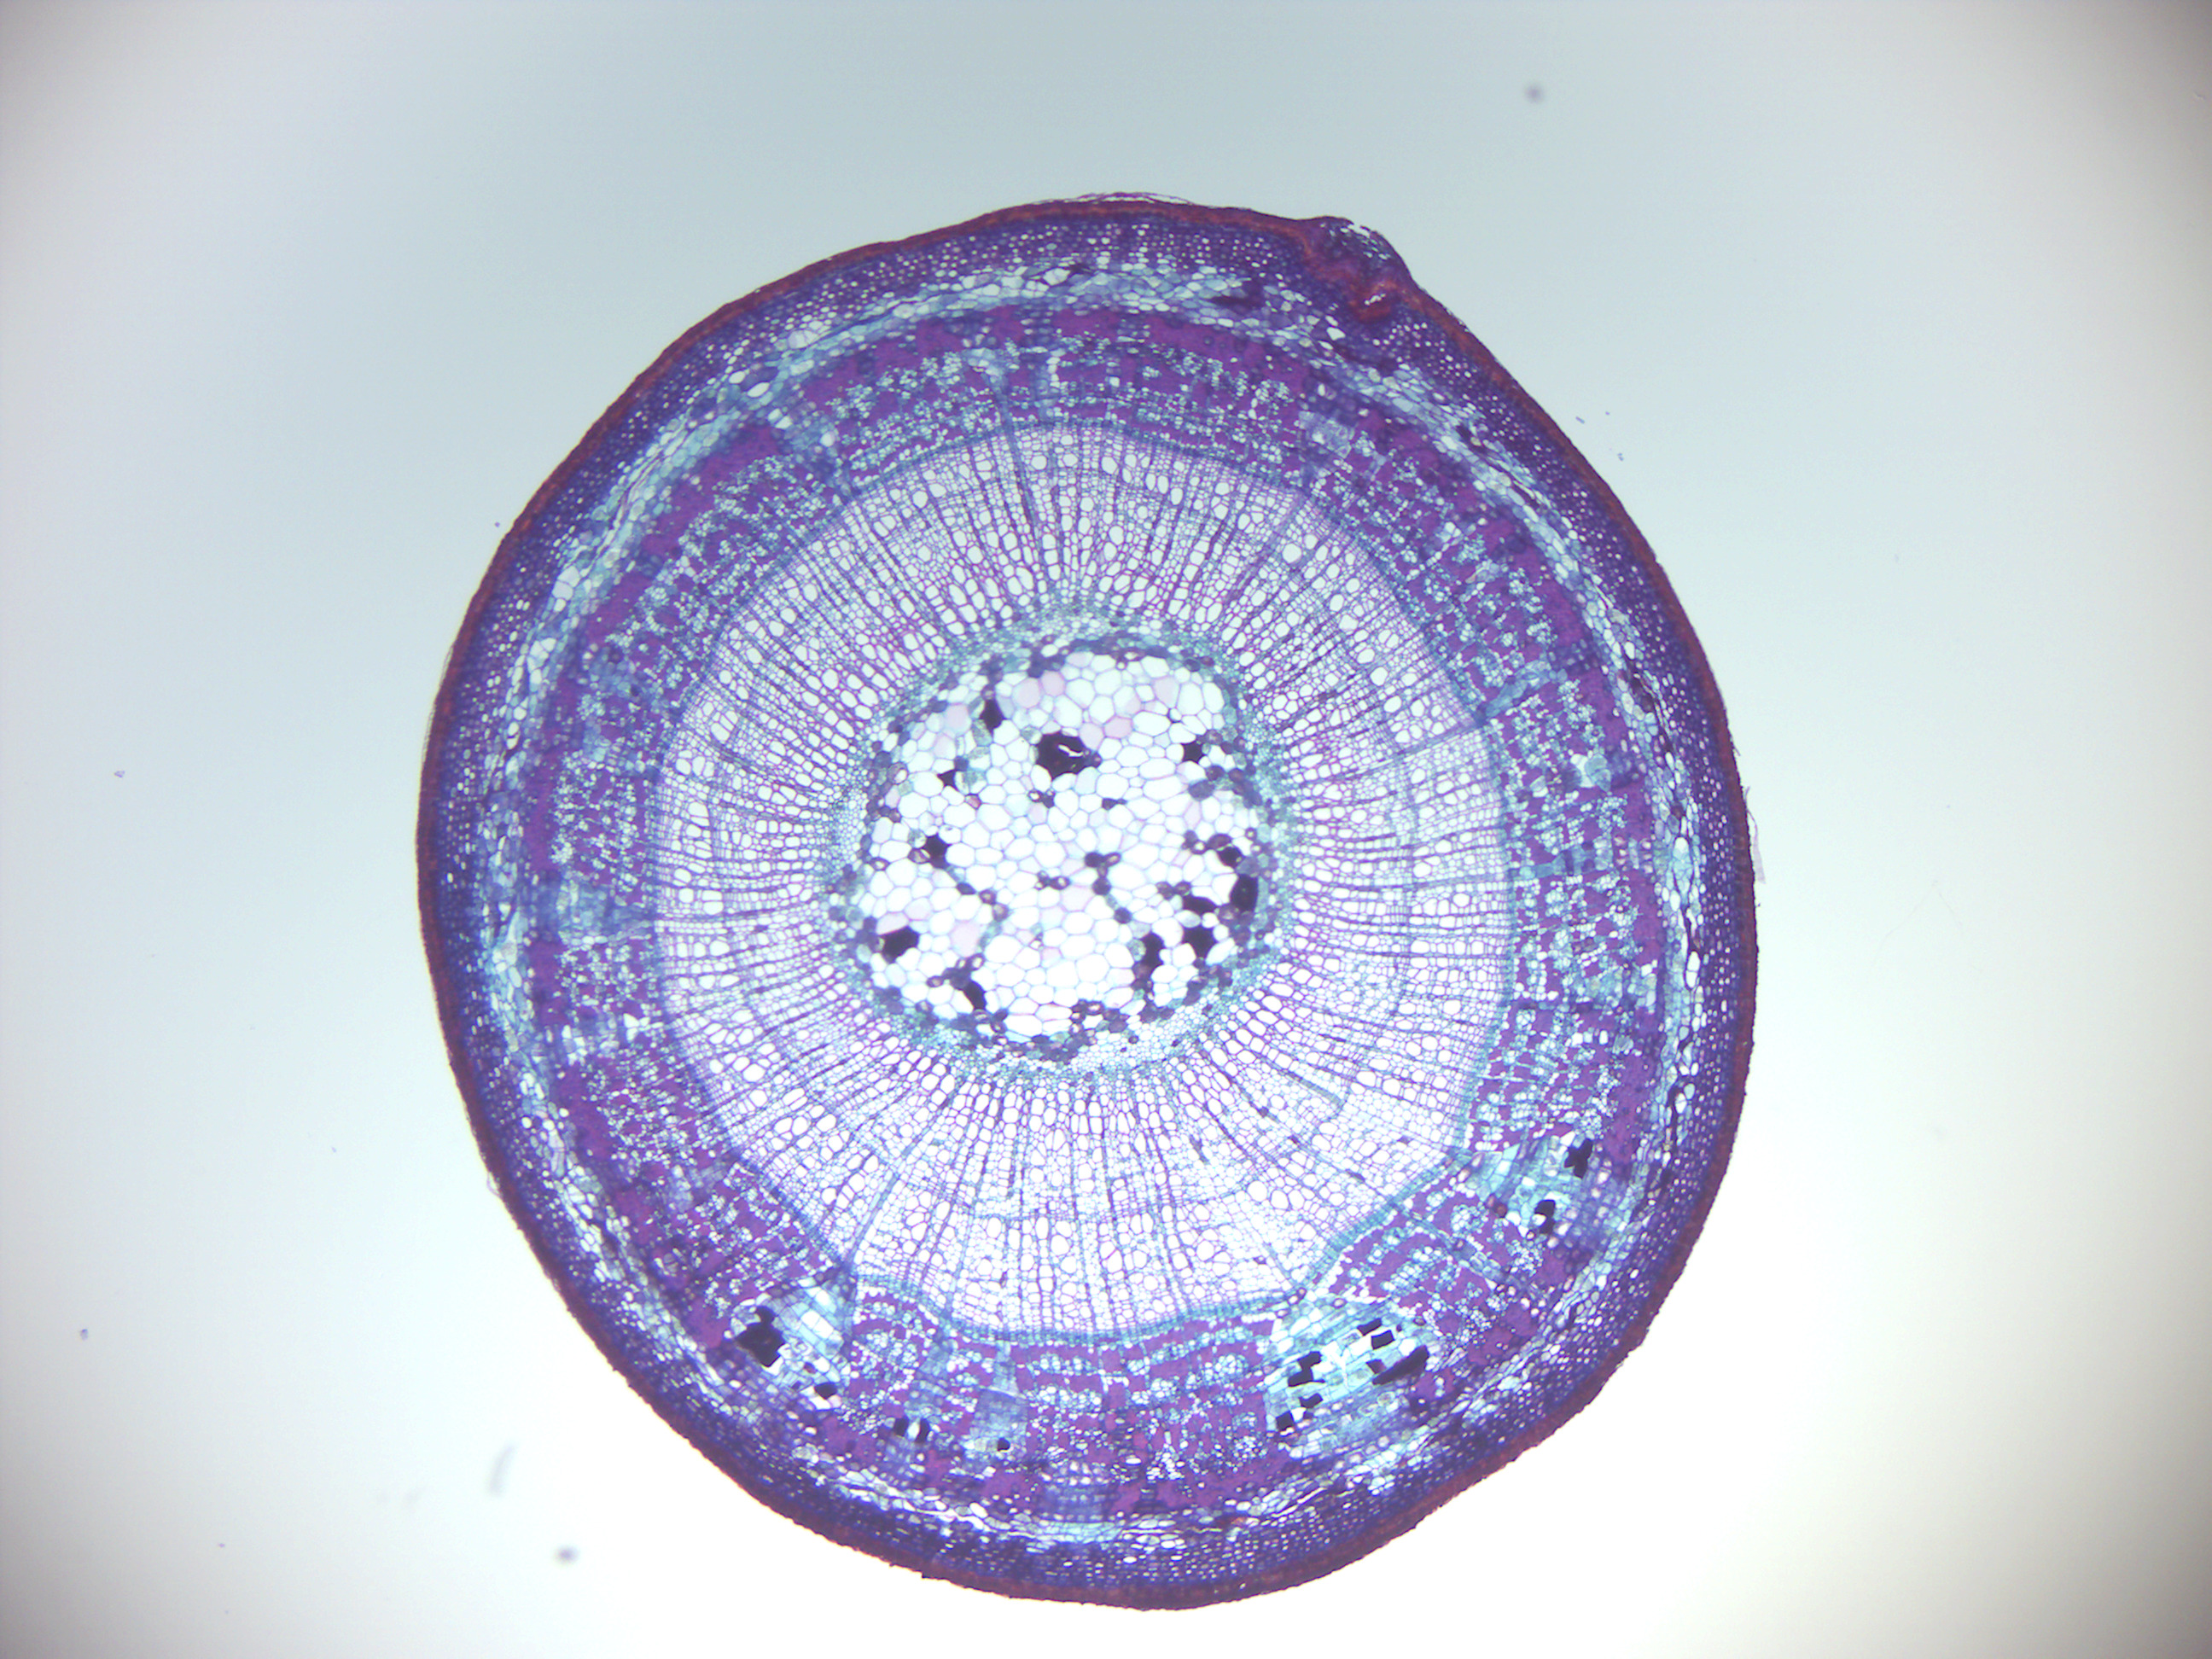
\includegraphics[width=0.7\linewidth]{./figures/gymnosperms/tilia}

}

\caption{\emph{Tilia} 2 year old stem}\label{fig:tilia}
\end{figure}

\begin{figure}

{\centering 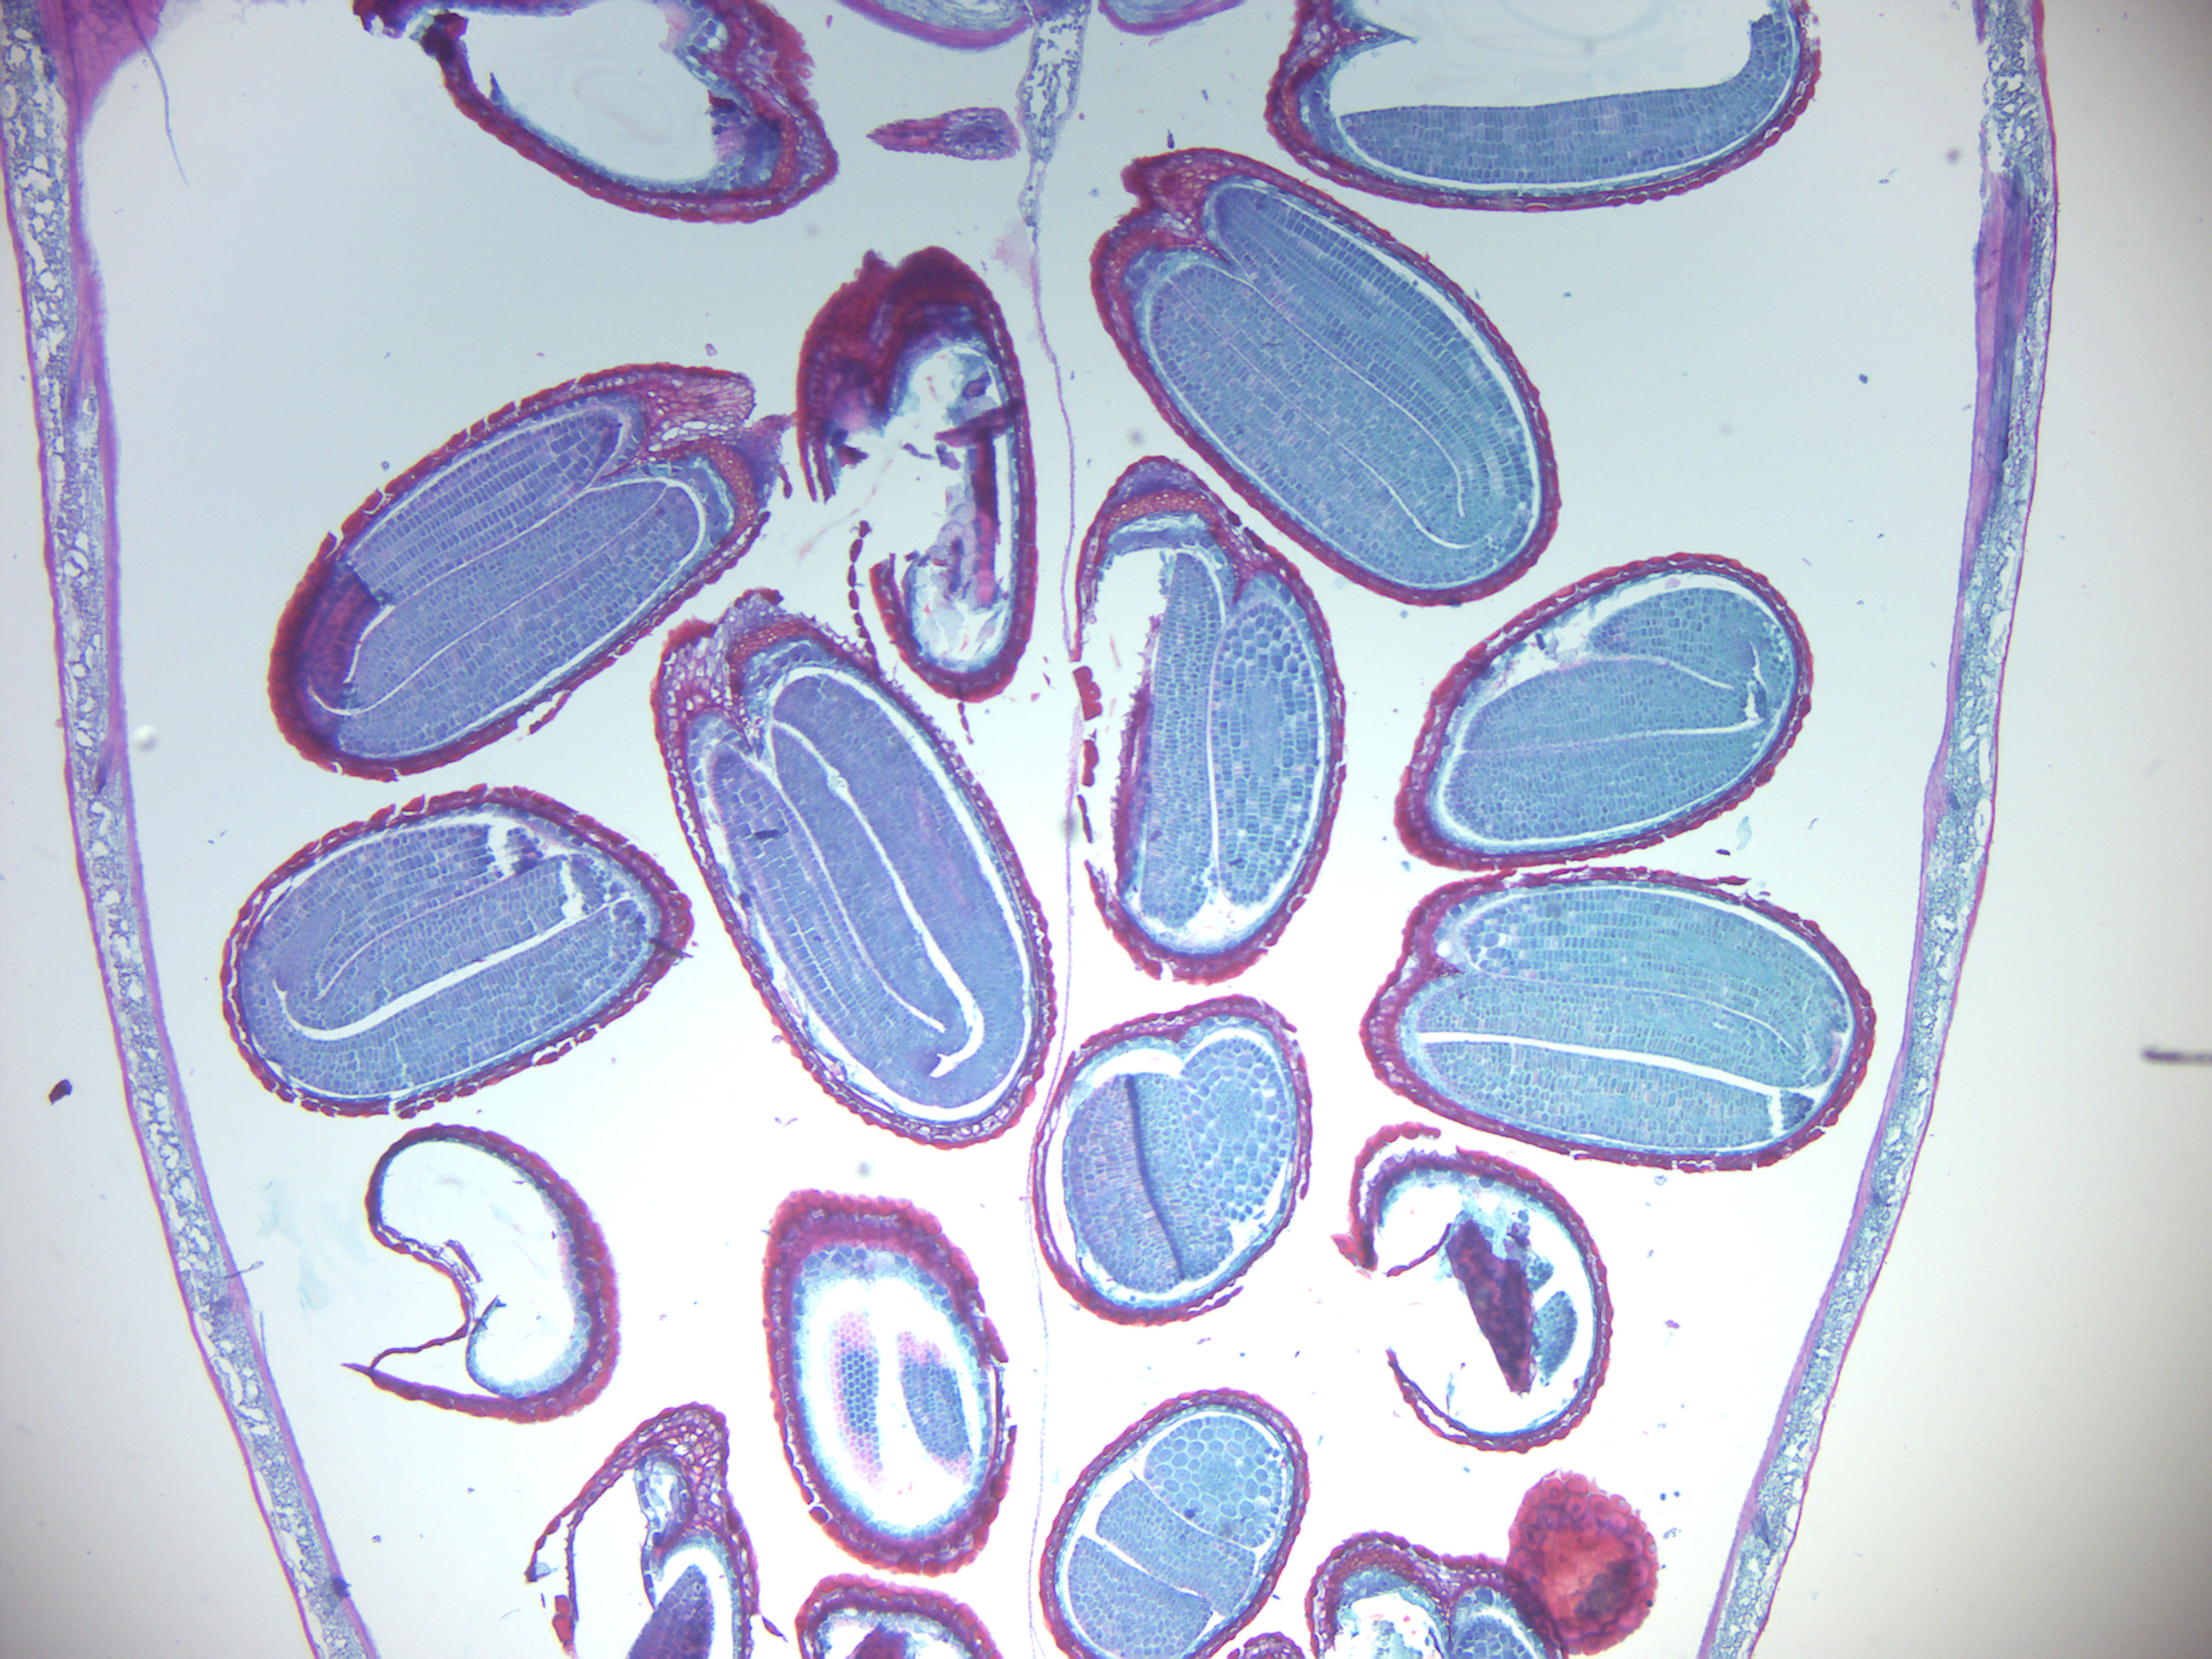
\includegraphics[width=0.7\linewidth]{./figures/gymnosperms/capsella_embryo}

}

\caption{\emph{Capsella} seeds.}\label{fig:capsella}
\end{figure}

\section{Monocotyledons and
Dicotyledons}\label{monocotyledons-and-dicotyledons}

Monocotyledons, commonly referred to as monocots are flowering plants
(angiosperms) whose seeds typically contain only one embryonic leaf, or
cotyledon. They constitute one of the major groups into which the
flowering plants have traditionally been divided, the rest of the
flowering plants having two cotyledons and therefore classified as
dicotyledons, or dicots. However, molecular phylogenetic research has
shown that while the monocots form a monophyletic group or clade
(comprising all the descendants of a common ancestor), the dicots do
not.

The eudicots, eudicotyledons are a monophyletic clade of flowering
plants. The term means ``true dicotyledons'', as it contains the
majority of plants that have been considered dicots and have
characteristics of the dicots. The term ``eudicots'' has subsequently
been widely adopted in botany to refer to one of the two largest clades
of angiosperms (constituting over 70\% of the angiosperm species),
monocots being the other.

\begin{longtable}[]{@{}lll@{}}
\caption{\label{tab:moncots} Structural differences between monocots and
dicots.}\tabularnewline
\toprule
\begin{minipage}[b]{0.10\columnwidth}\raggedright\strut
Feature\strut
\end{minipage} & \begin{minipage}[b]{0.40\columnwidth}\raggedright\strut
In monocots\strut
\end{minipage} & \begin{minipage}[b]{0.40\columnwidth}\raggedright\strut
In dicots\strut
\end{minipage}\tabularnewline
\midrule
\endfirsthead
\toprule
\begin{minipage}[b]{0.10\columnwidth}\raggedright\strut
Feature\strut
\end{minipage} & \begin{minipage}[b]{0.40\columnwidth}\raggedright\strut
In monocots\strut
\end{minipage} & \begin{minipage}[b]{0.40\columnwidth}\raggedright\strut
In dicots\strut
\end{minipage}\tabularnewline
\midrule
\endhead
\begin{minipage}[t]{0.10\columnwidth}\raggedright\strut
Leaves\strut
\end{minipage} & \begin{minipage}[t]{0.40\columnwidth}\raggedright\strut
Leaf shape oblong or linear, often sheathed at base, petiole seldom
developed, stipules absent. Major leaf veins usually parallel.\strut
\end{minipage} & \begin{minipage}[t]{0.40\columnwidth}\raggedright\strut
Broad, seldom sheathed, petiole common often with stipules. Veins
usually reticulate (pinnate or palmate).\strut
\end{minipage}\tabularnewline
\begin{minipage}[t]{0.10\columnwidth}\raggedright\strut
Roots\strut
\end{minipage} & \begin{minipage}[t]{0.40\columnwidth}\raggedright\strut
Primary root of short duration, replaced by adventitial roots forming
fibrous or fleshy root systems.\strut
\end{minipage} & \begin{minipage}[t]{0.40\columnwidth}\raggedright\strut
Develops from the radicle. Primary root often persists forming strong
taproot and secondary roots.\strut
\end{minipage}\tabularnewline
\begin{minipage}[t]{0.10\columnwidth}\raggedright\strut
Plant stem: Vascular bundles\strut
\end{minipage} & \begin{minipage}[t]{0.40\columnwidth}\raggedright\strut
Numerous scattered bundles in ground parenchyma, cambium rarely present,
no differentiation between cortical and stelar regions.\strut
\end{minipage} & \begin{minipage}[t]{0.40\columnwidth}\raggedright\strut
Ring of primary bundles with cambium, differentiated into cortex and
stele (eustelic).\strut
\end{minipage}\tabularnewline
\begin{minipage}[t]{0.10\columnwidth}\raggedright\strut
Flowers\strut
\end{minipage} & \begin{minipage}[t]{0.40\columnwidth}\raggedright\strut
Parts in threes or multiples of three (e.g.~3, 6 or 9 petals)\strut
\end{minipage} & \begin{minipage}[t]{0.40\columnwidth}\raggedright\strut
Parts in fours or fives.\strut
\end{minipage}\tabularnewline
\bottomrule
\end{longtable}

\section{View Prepared Slides of Monocots And
Eudicots}\label{view-prepared-slides-of-monocots-and-eudicots}

\begin{enumerate}
\def\labelenumi{\arabic{enumi}.}
\tightlist
\item
  Monocot and dicot roots (Figures \ref{fig:monocotroot} and
  \ref{fig:dicotroot})

  \begin{itemize}
  \tightlist
  \item
    Identify monocot and eudicot root.
  \end{itemize}
\item
  Monocot and dicot stems (Figures \ref{fig:monocotstem} and
  \ref{fig:dicotstem})

  \begin{itemize}
  \tightlist
  \item
    Identify monocot and eudicot sterm.
  \end{itemize}
\item
  Monocot and dicot leaves (Figures \ref{fig:monocotleave} and
  \ref{fig:dicotleave})

  \begin{itemize}
  \tightlist
  \item
    Identify monocot and eudicot leaf.
  \end{itemize}
\item
  Monocot and dicot flower buds (Figures \ref{fig:monocotbud} and
  \ref{fig:dicotbud})

  \begin{itemize}
  \tightlist
  \item
    Identify monocot and eudicot flower.
  \end{itemize}
\end{enumerate}

\begin{figure}

{\centering 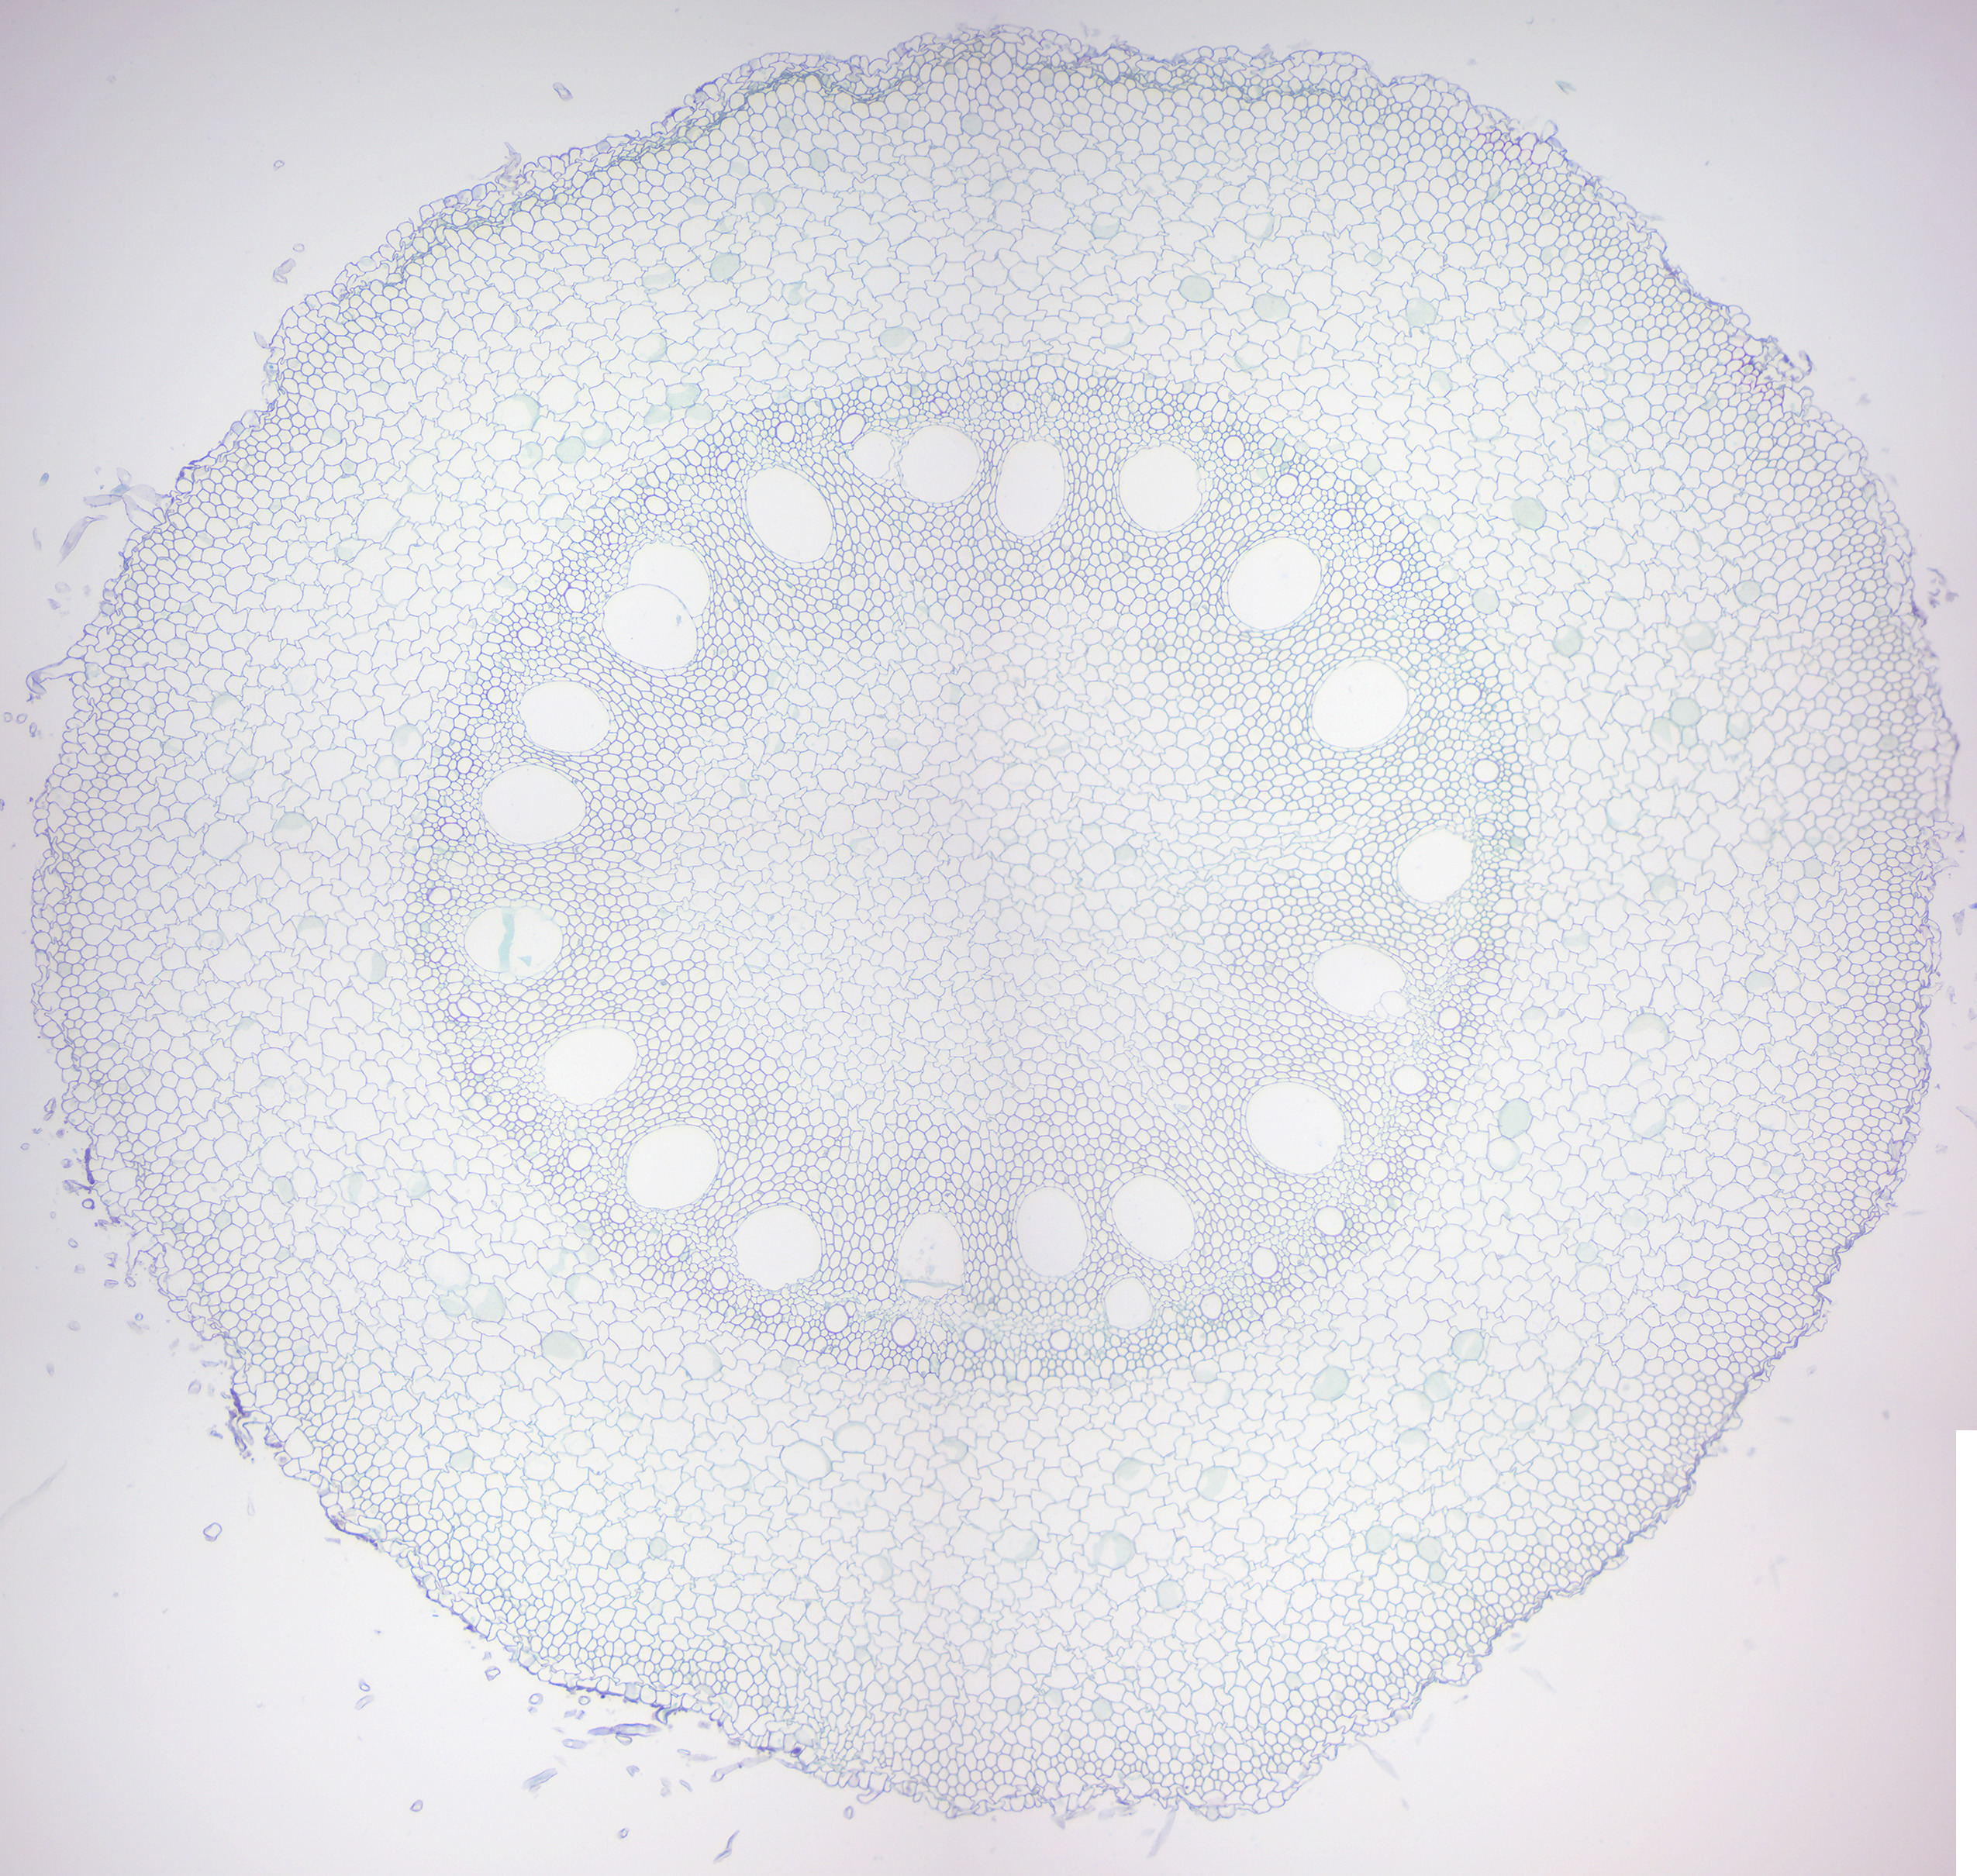
\includegraphics[width=0.7\linewidth]{./figures/gymnosperms/monocot_root}

}

\caption{Monocot root.}\label{fig:monocotroot}
\end{figure}

\begin{figure}

{\centering 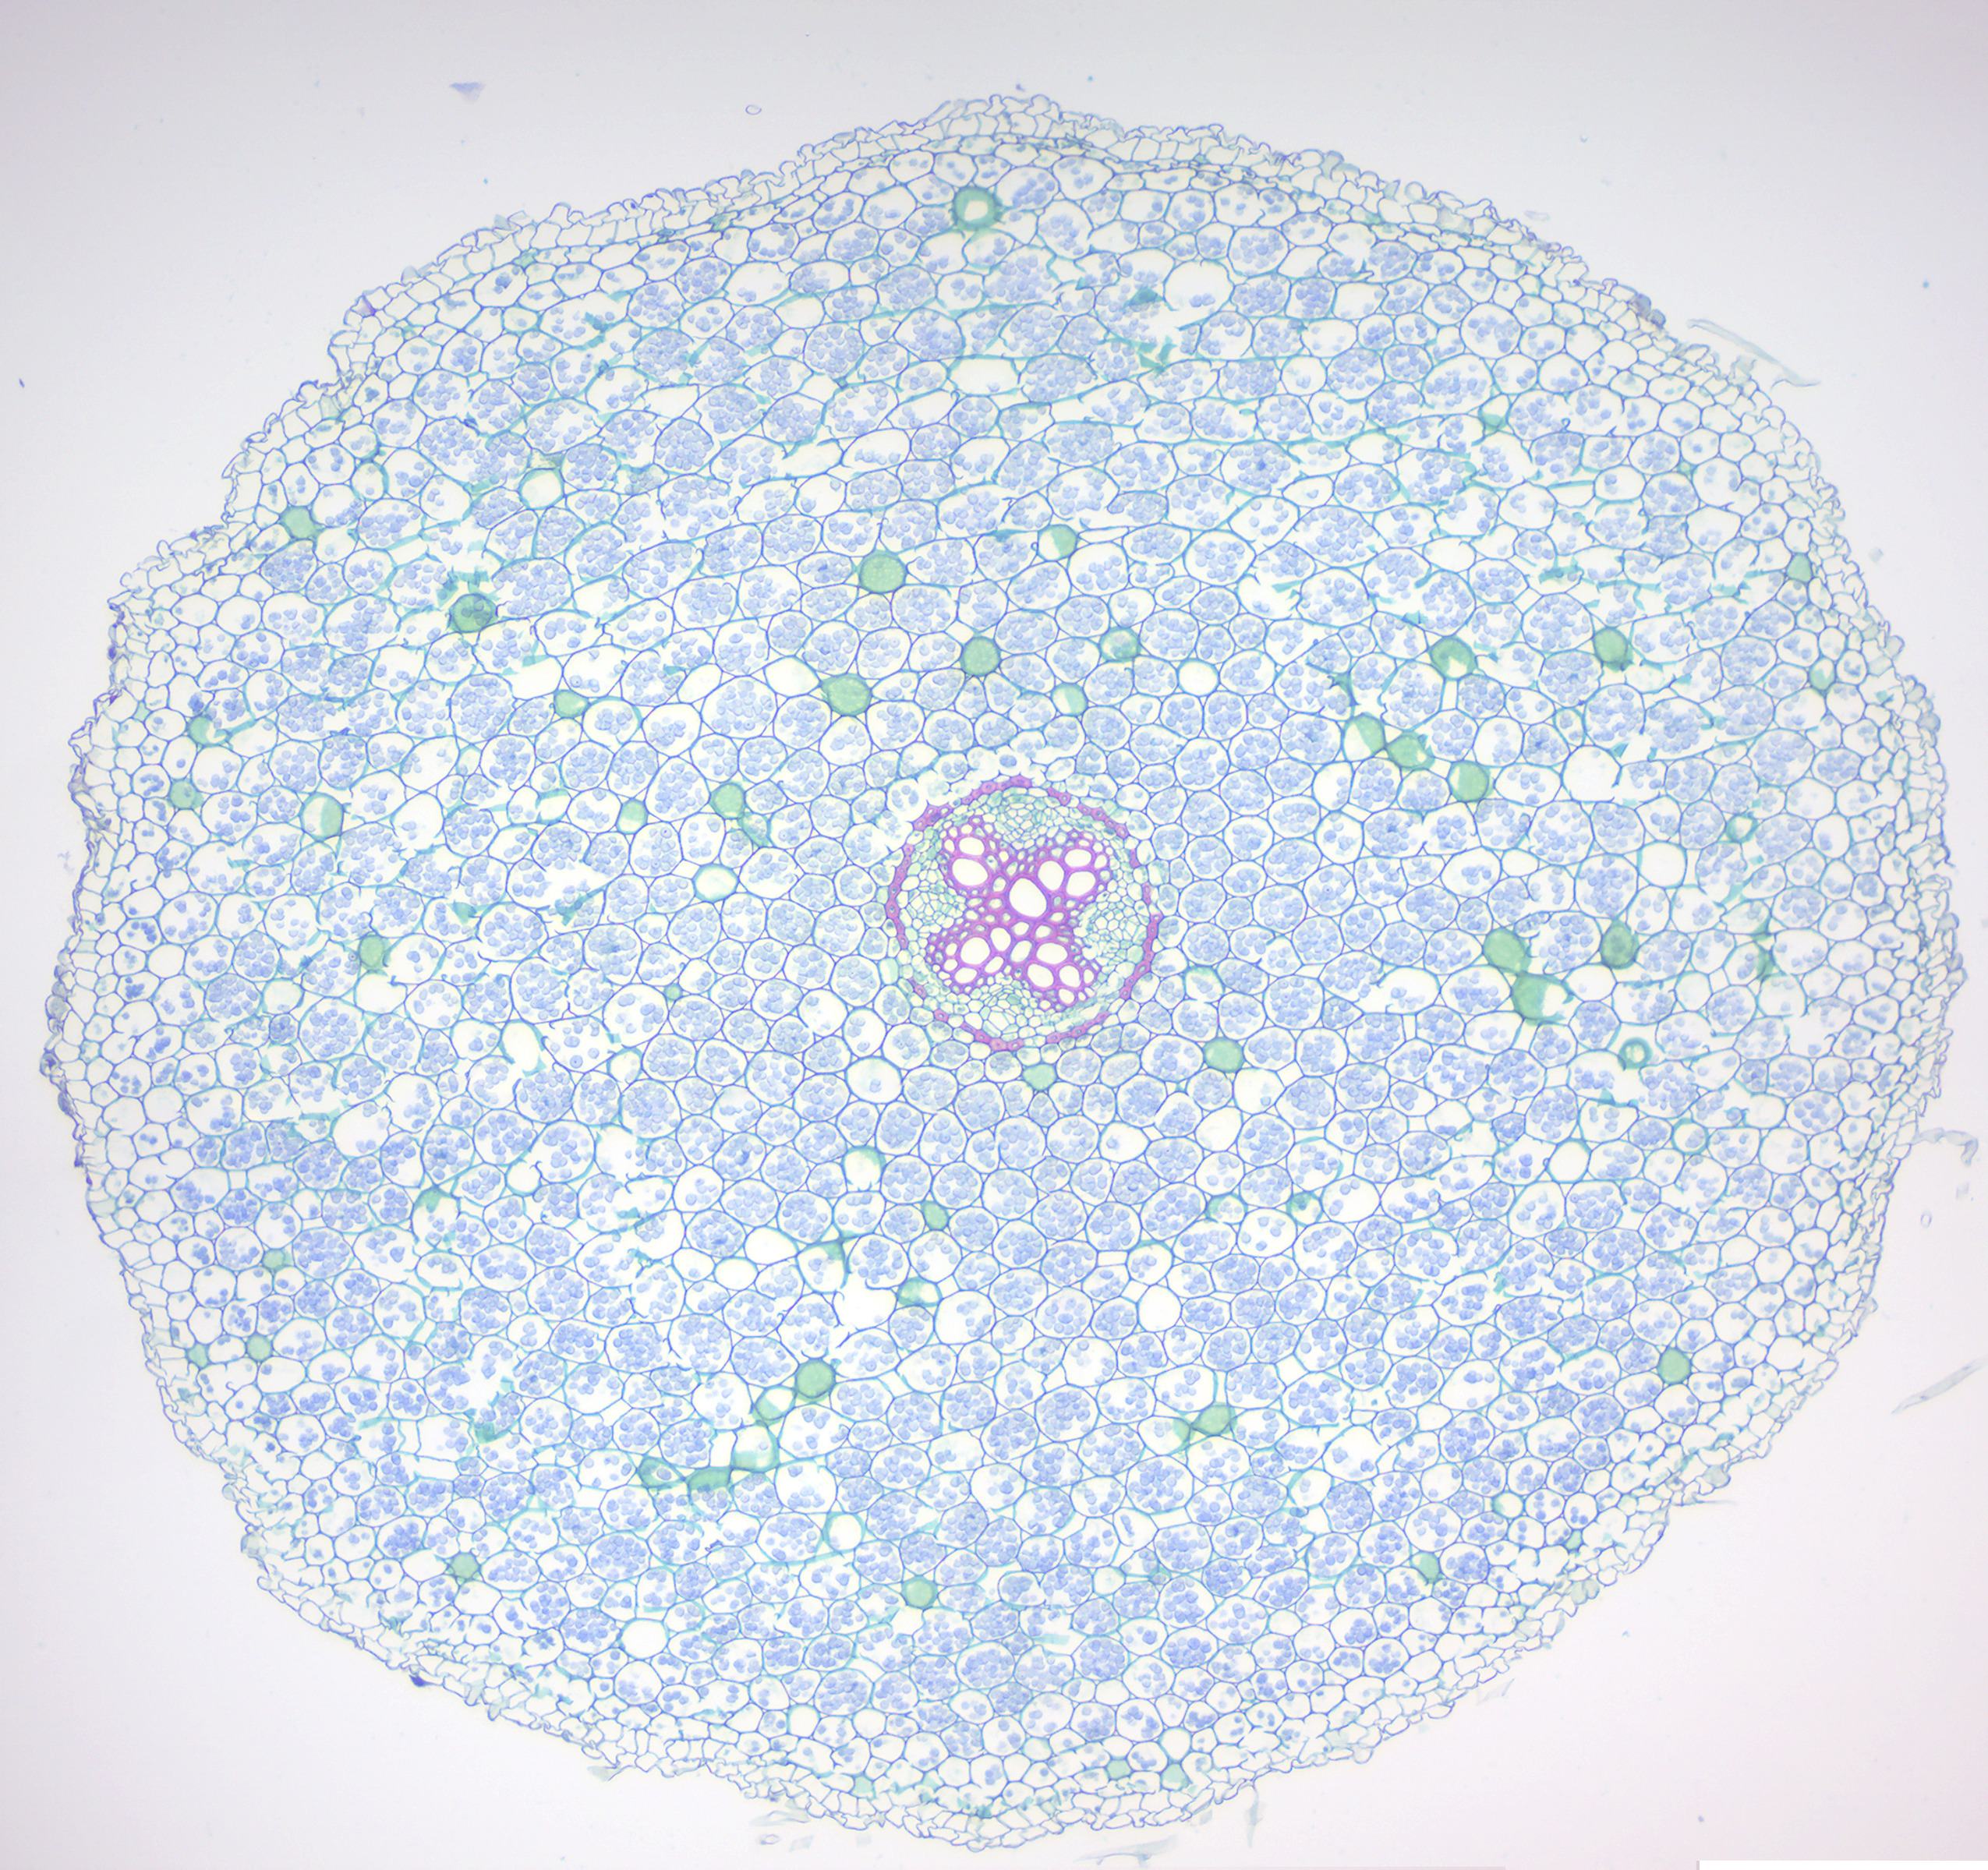
\includegraphics[width=0.7\linewidth]{./figures/gymnosperms/Dicot_root}

}

\caption{Dicot root.}\label{fig:dicotroot}
\end{figure}

\begin{figure}

{\centering 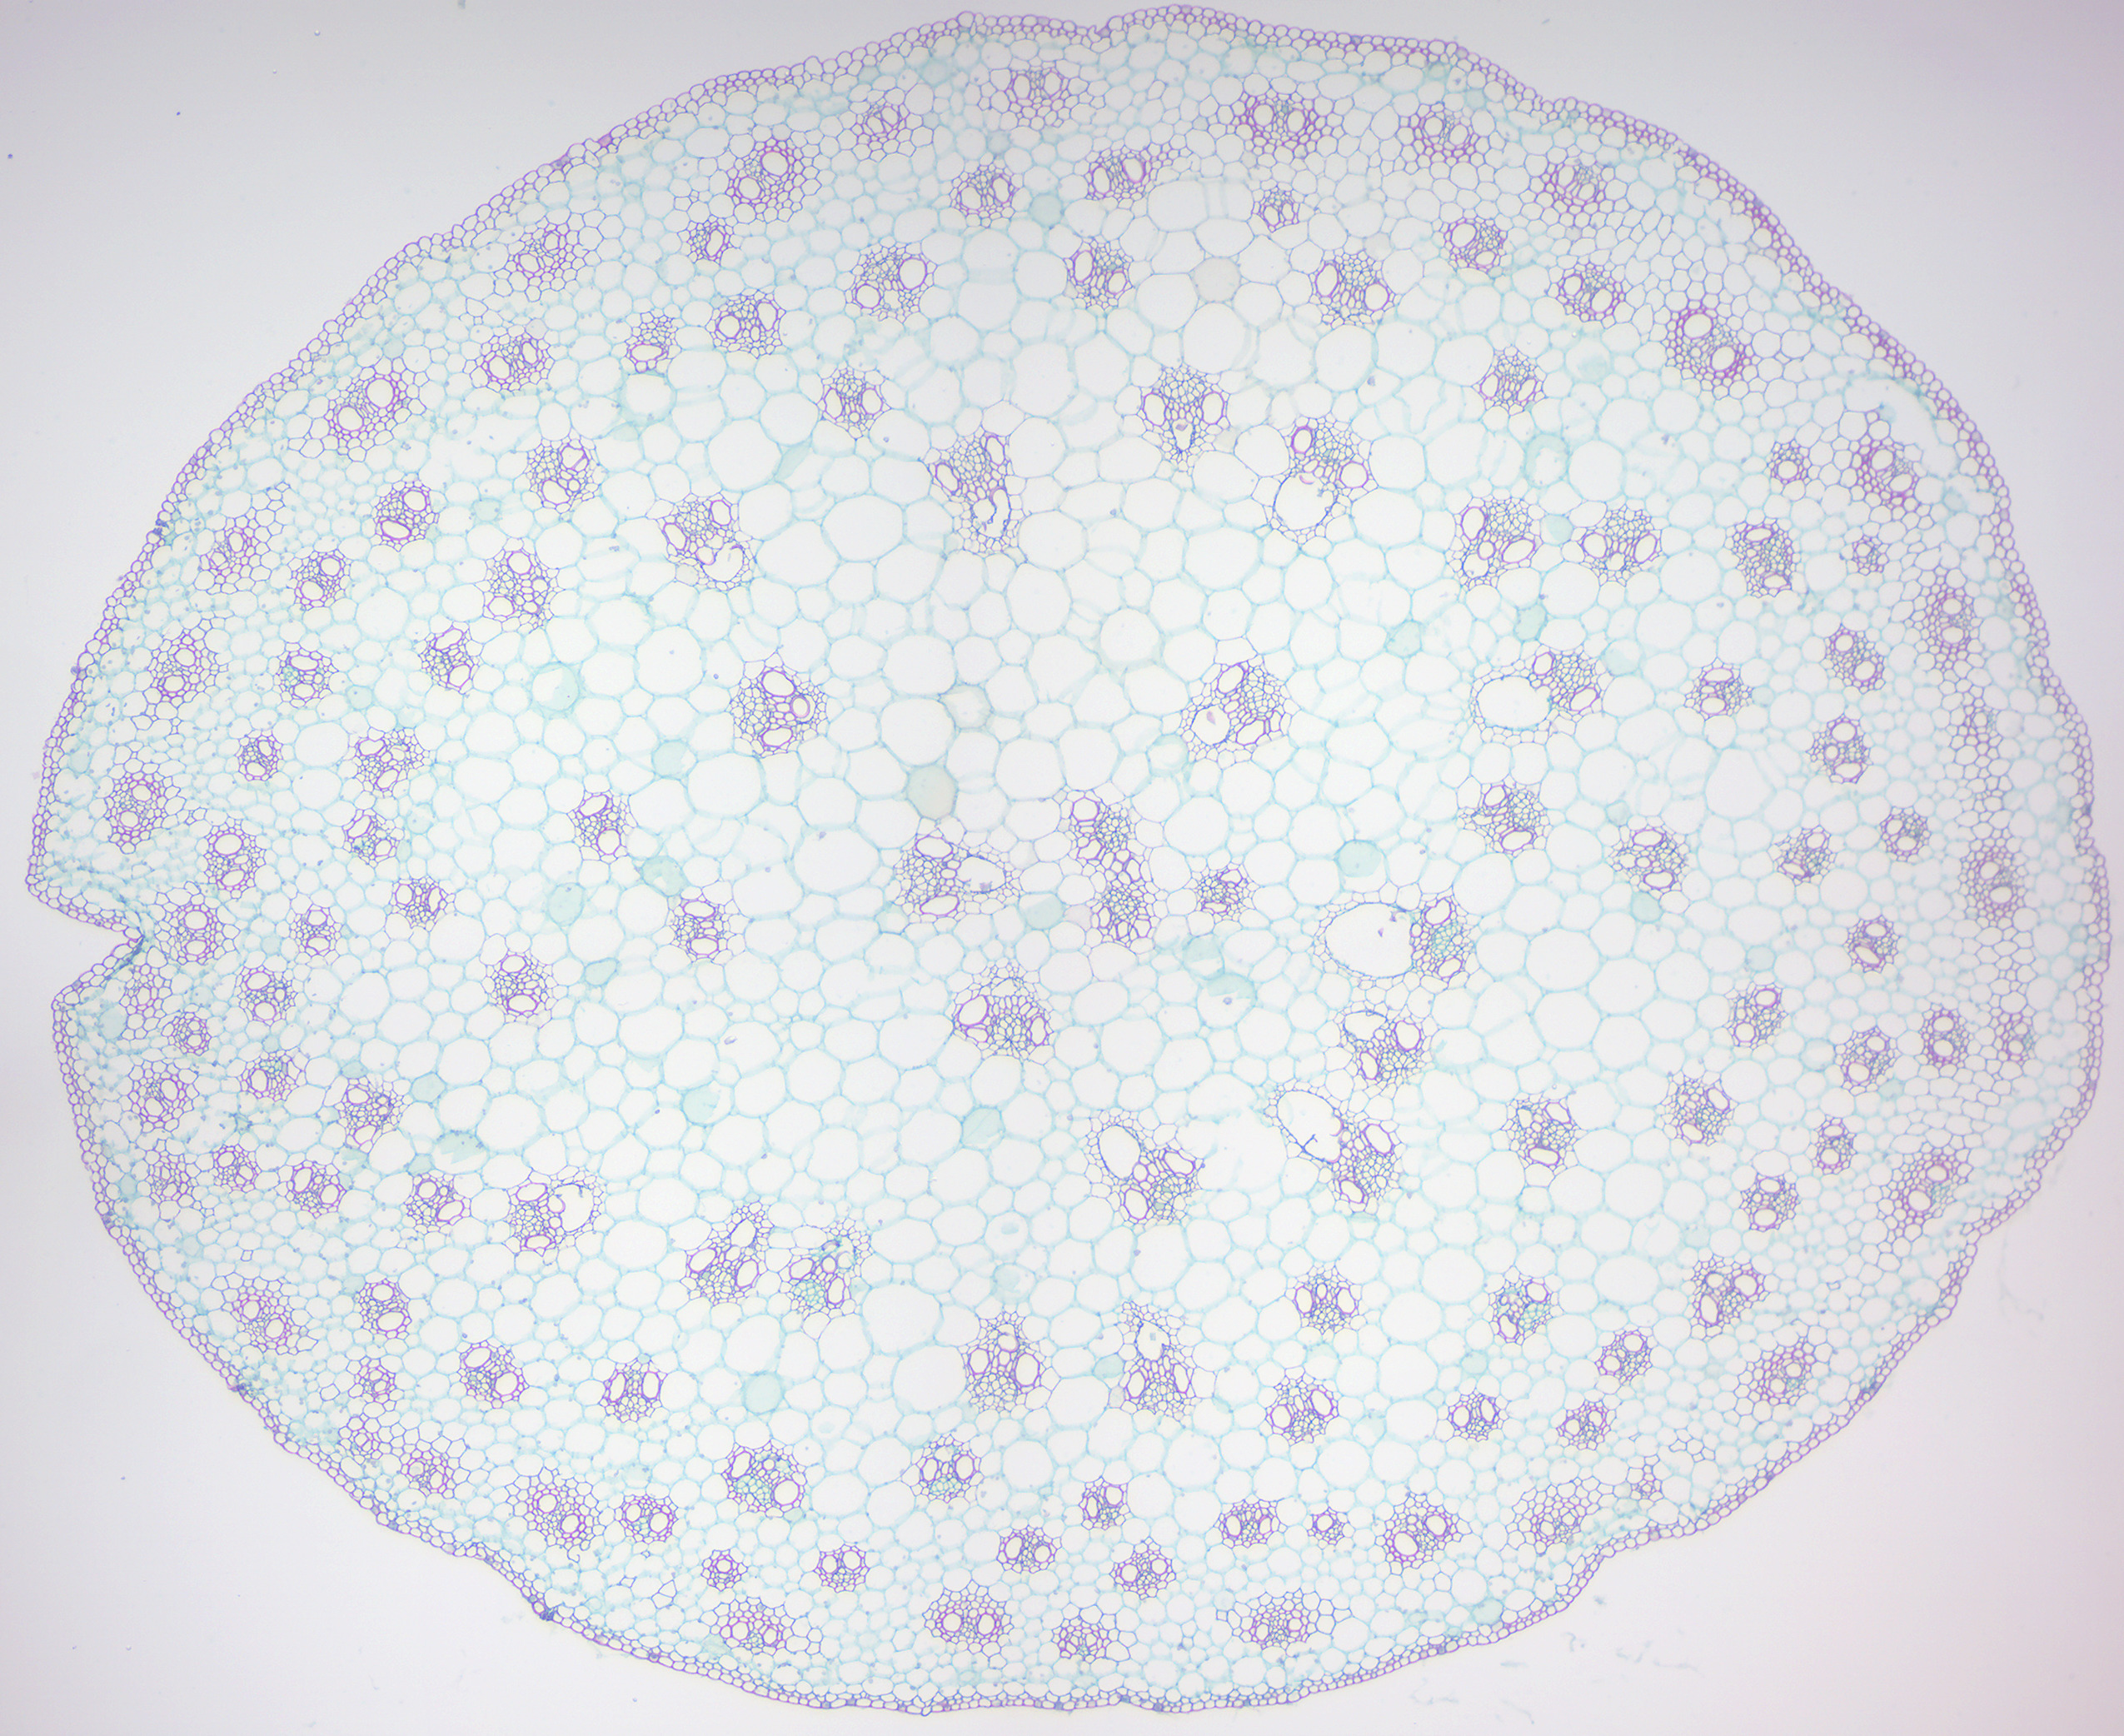
\includegraphics[width=0.7\linewidth]{./figures/gymnosperms/monocot_stem}

}

\caption{Monocot stem.}\label{fig:monocotstem}
\end{figure}

\begin{figure}

{\centering 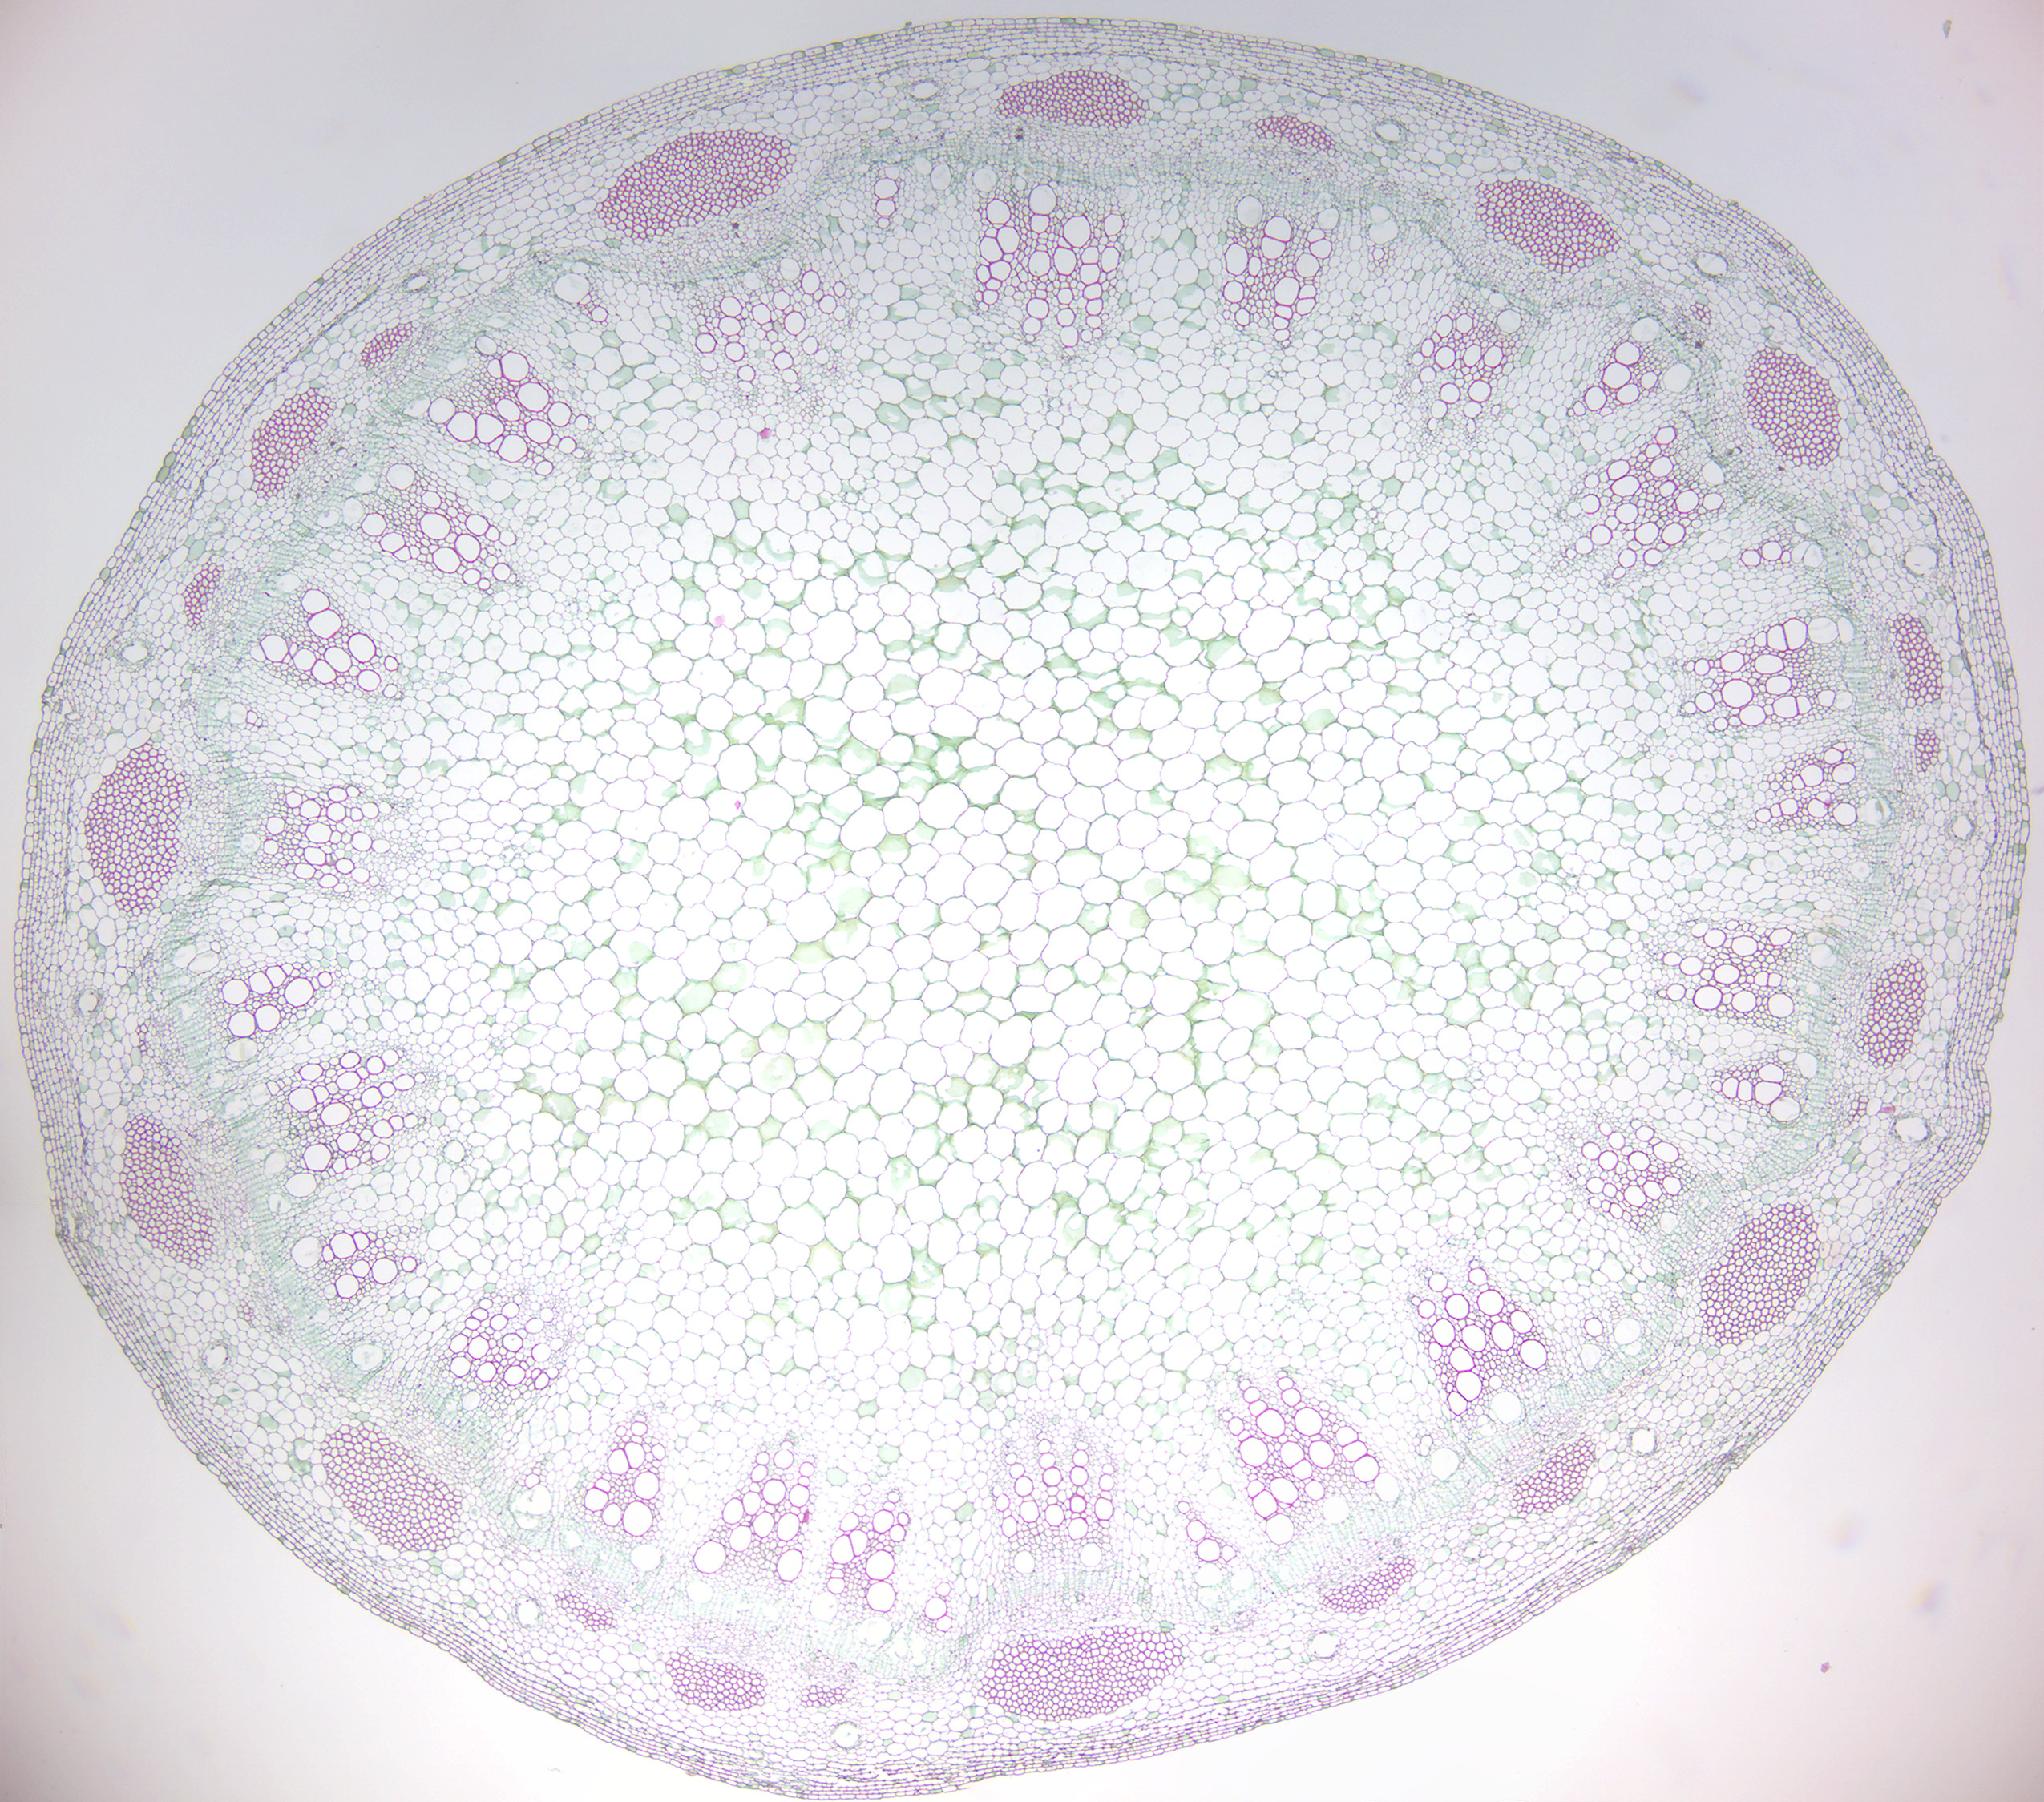
\includegraphics[width=0.7\linewidth]{./figures/gymnosperms/dicot_stem}

}

\caption{Dicot stem}\label{fig:dicotstem}
\end{figure}

\begin{figure}

{\centering 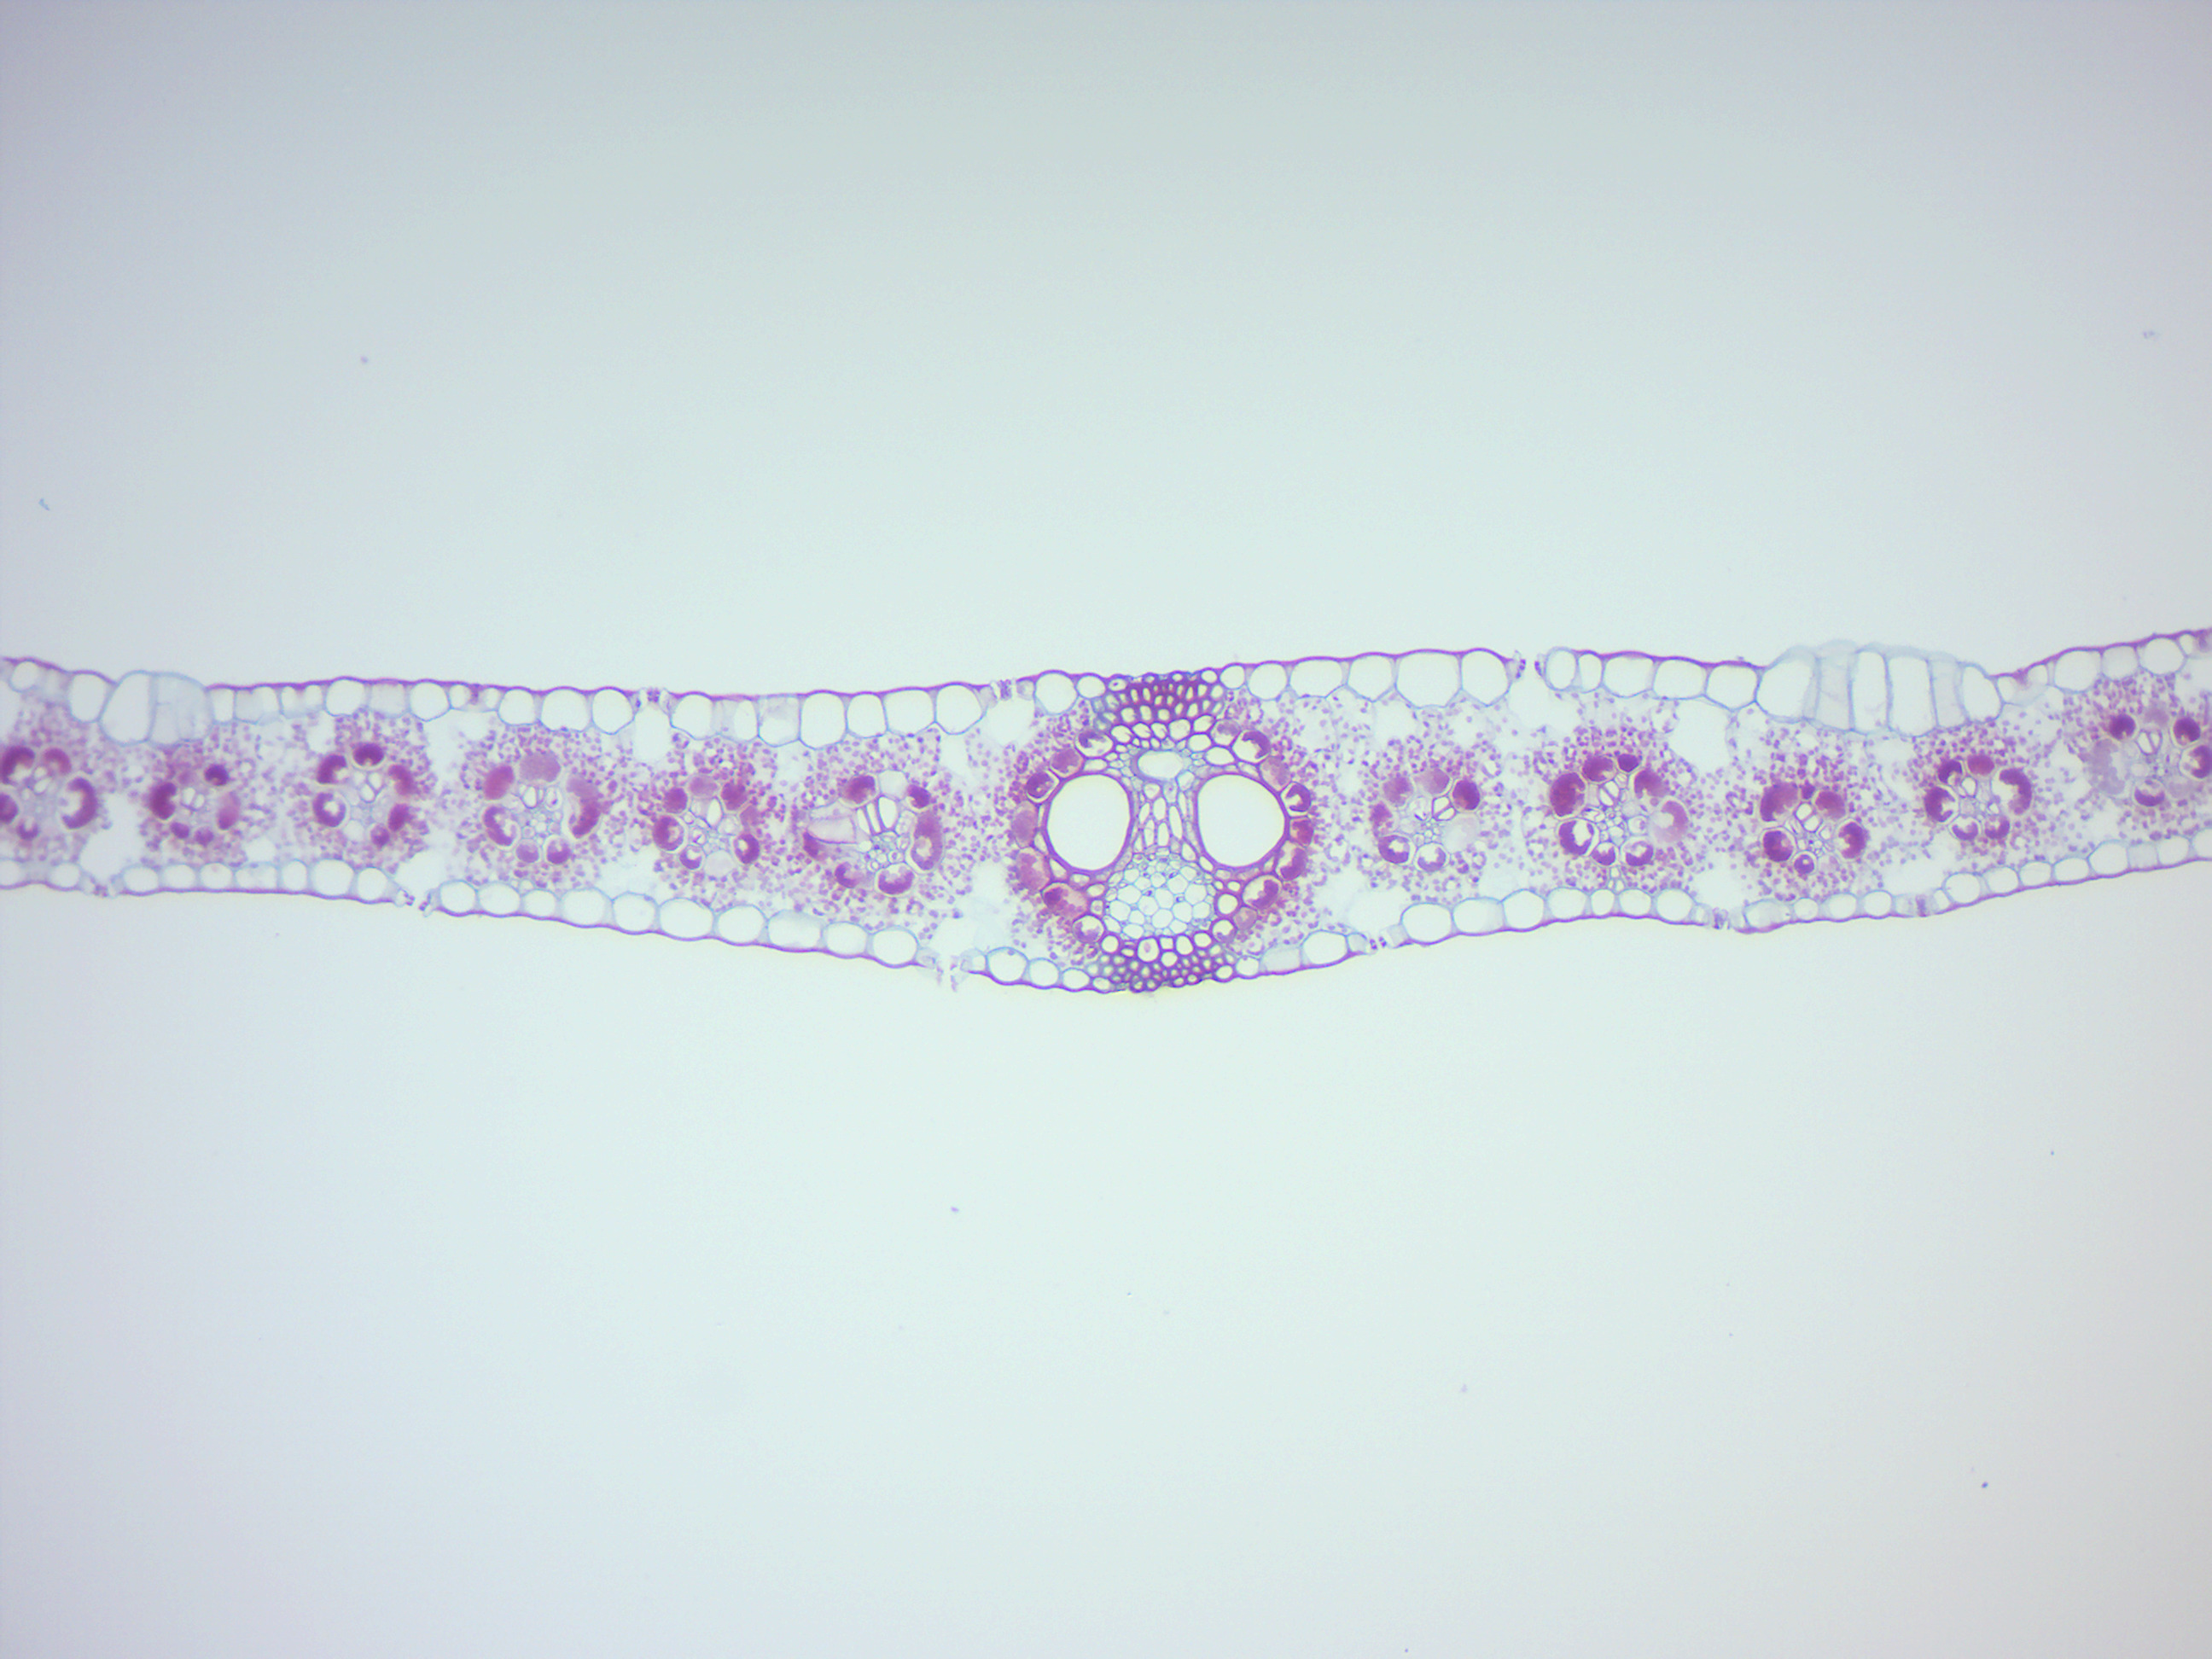
\includegraphics[width=0.7\linewidth]{./figures/gymnosperms/monocot_leave}

}

\caption{Monocot leave.}\label{fig:monocotleave}
\end{figure}

\begin{figure}

{\centering \includegraphics[width=0.7\linewidth]{./figures/gymnosperms/dicot_leave}

}

\caption{Dicot leave.}\label{fig:dicotleave}
\end{figure}

\begin{figure}

{\centering \includegraphics[width=0.7\linewidth]{./figures/gymnosperms/monocot_flower_bud}

}

\caption{Monocot flower bud.}\label{fig:monocotbud}
\end{figure}

\begin{figure}

{\centering \includegraphics[width=0.7\linewidth]{./figures/gymnosperms/dicot_flower_bud}

}

\caption{Dicot flower bud.}\label{fig:dicotbud}
\end{figure}

\pagebreak

\section{\texorpdfstring{\emph{Lilium}}{Lilium}}\label{lilium}

\emph{Lilium} is a genus of herbaceous flowering plants growing from
bulbs, all with large prominent flowers. Lilies are a group of flowering
plants which are important in culture and literature in much of the
world. Most species are native to the temperate northern hemisphere,
though their range extends into the northern subtropics. Lilies are
tall perennials ranging in height from 2--6 ft.

\begin{figure}

{\centering \includegraphics[width=0.7\linewidth]{./figures/gymnosperms/lily}

}

\caption{Lilies}\label{fig:Lilies}
\end{figure}

The flowers are large, often fragrant, and come in a wide range of
colors including whites, yellows, oranges, pinks, reds and purples.
Markings include spots and brush strokes. The plants are late spring- or
summer-flowering. Flowers are at the tip of the stem, with six tepals
(sepals and petals are not distinct). The tepals are free from each
other, and bear a nectary at the base of each flower. The ovary is
`superior', borne above the point of attachment of the anthers. The
fruit is a three-celled capsule. Seeds ripen in late summer. They
exhibit varying and sometimes complex germination patterns, many adapted
to cool temperate climates. 

\section{Dissection of Fresh Lilies}\label{dissection-of-fresh-lilies}

\begin{enumerate}
\def\labelenumi{\arabic{enumi}.}
\tightlist
\item
  The outer ring of the flower consists of sepals, and the inner ring of
  petals. In lilies they look nearly identical. In many other flowers,
  the sepals are green and the petals are colorful.
\item
  Peel off first the sepals and then the petals.
\item
  Count the number of sepals and petals. Do you notice any (orange
  colored) pollen on any of them?
\item
  After you have peeled away the sepals and petals, you can clearly see
  the stamens (the ``male'' parts of the flower). The stamens mostly
  consist of anthers (the long, elliptical and brown heads on top of the
  filaments (the supporting stalks). Some anthers may have split open to
  expose othe pollen grains inside.
\item
  Cut off the stamens and examine the anther and pollen using the stereo
  dissection microscope.
\item
  The long stalk remainin in the center of the flower is the pistil (the
  ``female'' parts) with the stigma at its top end. If the flowers are
  fresh, the stigma will be sticky for catching pollen. You can cut it
  open along the path down the style (the stalky part), to the ovule.
\item
  At the base of the style is the ovary. It contains the ovules that
  will develop into vseeds if they are fertilized by sperm from the
  pollen.
\item
  Cut the ovary in half to see the ovules.
\item
  Examine the cut ovary using the stereo dissection microscope.
\item
  At the base of the the ovary is the main nectary. Cut it open to see
  the xylem (the water conducting vessels of vascular plants) and phloem
  (the sugar conductiong vessels).
\end{enumerate}

\section{Review Questions}\label{review-questions-2}

\begin{enumerate}
\def\labelenumi{\arabic{enumi}.}
\tightlist
\item
  What are gymnosperms?
\item
  What are angiosperms?
\item
  What are pollen?
\item
  What are cotyledons?
\item
  What is xylem?
\item
  What is phloem?
\end{enumerate}

\chapter{Porifera, Cnidaria,
Ctenophora}\label{porifera-cnidaria-ctenophora}

\section{Animals}\label{animals}

\href{https://en.wikipedia.org/wiki/Animal}{Animals} are eukaryotic,
multicellular organisms that form the biological kingdom Animalia. With
few exceptions, animals are motile (able to move), heterotrophic
(consume organic material), reproduce sexually, and their embryonic
development includes a blastula stage. The body plan of the animal
derives from this blastula, differentiating specialized tissues and
organs as it develops; this plan eventually becomes fixed, although some
undergo metamorphosis at some stage in their lives.

Zoology is the study of animals. Currently there are over 66,000
(less than 5\% of all animals) vertebrate species, and over 1.3 million
(over 95\% of all animals) invertebrate species in existence.
Classification of animals into groups (taxonomy) is accomplished using
either the hierarchical Linnaean system; or cladistics, which displays
diagrams (phylogenetic trees) called cladograms to show relationships
based on the evolutionary principle of the most recent common ancestor.
Some recent classifications based on modern cladistics have explicitly
abandoned the term ``kingdom'', noting that the traditional kingdoms are
not monophyletic, i.e., do not consist of all the descendants of a
common ancestor.

Animals are divided by body plan into vertebrates and invertebrates.
Vertebrates---fishes, amphibians, reptiles, birds, and mammals---have a
vertebral column (spine); invertebrates do not. All vertebrates and most
invertebrates are bilaterally symmetrical (Bilateria). Invertebrates
include arthropods, molluscs, roundworms, ringed worms, flatworms, and
other phyla in Ecdysozoa and Spiralia. Echinoderm larvae are initially
bilaterally symmetrical, but later as adults develop radial symmetry;
Cnidarians are radially symmetrical; ctenophores are biradially
symmetrical; and sponges have no symmetry.

Animal phyla appeared in the fossil record as marine species during the
Cambrian explosion, about 542 million years ago. Animals emerged as a
clade within \ref{https://en.wikipedia.org/wiki/Apoikozoa}{Apoikozoa} as the sister group to the choanoflagellates.

\section{Poriphera}\label{poriphera}

\href{https://en.wikipedia.org/wiki/Sponge}{Sponges}, the members of the
phylum Porifera (meaning ``pore bearer''), are multicellular organisms
that have bodies full of pores and channels allowing water to circulate
through them, consisting of jelly-like mesohyl sandwiched between two
thin layers of cells. Sponges have unspecialized cells that can
transform into other types and that often migrate between the main cell
layers and the mesohyl in the process. Sponges do not have nervous,
digestive or circulatory systems. Instead, most rely on maintaining a
constant water flow through their bodies to obtain food and oxygen and
to remove wastes. Sponges are thought to be the first to branch off the
evolutionary tree from the common ancestor of all animals, making them
the sister group of all other animals.

The phylum Porifera is further divided into four classes mainly
according to the composition of their skeletons:

\begin{enumerate}
\def\labelenumi{\arabic{enumi}.}
\tightlist
\item
  Hexactinellida (glass sponges) have silicate spicules, the largest of
  which have six rays and may be individual or fused. The main
  components of their bodies are syncytia in which large numbers of cell
  share a single external membrane.
\item
  Calcarea have skeletons made of calcite, a form of calcium carbonate,
  which may form separate spicules or large masses. All the cells have a
  single nucleus and membrane.
\item
  Most Demospongiae have silicate spicules or spongin fibers or both
  within their soft tissues. However a few also have massive external
  skeletons made of aragonite, another form of calcium carbonate. All
  the cells have a single nucleus and membrane.
\item
  Archeocyatha are known only as fossils from the Cambrian period.
\end{enumerate}

Sponges are similar to other animals in that they are multicellular,
heterotrophic, lack cell walls and produce sperm cells. Unlike other
animals, they lack true tissues and organs, and have no body symmetry.
The shapes of their bodies are adapted for maximal efficiency of water
flow through the central cavity, where it deposits nutrients, and leaves
through a hole called the osculum. Many sponges have internal skeletons
of spongin and/or spicules of calcium carbonate or silicon dioxide. All
sponges are sessile aquatic animals. Although there are freshwater
species, the great majority are marine (salt water) species, ranging
from tidal zones to depths exceeding 8,800 m (5.5 mi).

While most of the approximately 5,000--10,000 known species feed on
bacteria and other food particles in the water, some host
photosynthesizing micro-organisms as endosymbionts and these alliances
often produce more food and oxygen than they consume. A few species of
sponge that live in food-poor environments have become carnivores that
prey mainly on small crustaceans.

\begin{figure}

{\centering \includegraphics[width=0.7\linewidth]{./figures/porifera/sponges}

}

\caption{Sponges and corals.}\label{fig:sponges}
\end{figure}

Sponges in temperate regions live for at most a few years, but some
tropical species and perhaps some deep-ocean ones may live for 200 years
or more. Some calcified demosponges grow by only 0.2 mm (0.0079 in) per
year and, if that rate is constant, specimens 1 m (3.3 ft) wide must be
about 5,000 years old. Some sponges start sexual reproduction when only
a few weeks old, while others wait until they are several years old.

Most species use sexual reproduction, releasing sperm cells into the
water to fertilize ova that in some species are released and in others
are retained by the ``mother''. The fertilized eggs form larvae which
swim off in search of places to settle. Sponges are known for
regenerating from fragments that are broken off, although this only
works if the fragments include the right types of cells. A few species
reproduce by budding. When conditions deteriorate, for example as
temperatures drop, many freshwater species and a few marine ones produce
gemmules, ``survival pods'' of unspecialized cells that remain dormant
until conditions improve and then either form completely new sponges or
recolonize the skeletons of their parents.

The mesohyl functions as an endoskeleton in most sponges, and is the
only skeleton in soft sponges that encrust hard surfaces such as rocks.
More commonly, the mesohyl is stiffened by mineral spicules, by spongin
fibers or both. Demosponges use spongin, and in many species, silica
spicules and in some species, calcium carbonate exoskeletons.
Demosponges constitute about 90\% of all known sponge species, including
all freshwater ones, and have the widest range of habitats. Calcareous
sponges, which have calcium carbonate spicules and, in some species,
calcium carbonate exoskeletons, are restricted to relatively shallow
marine waters where production of calcium carbonate is easiest. The
fragile glass sponges, with ``scaffolding'' of silica spicules, are
restricted to polar regions and the ocean depths where predators are
rare. Fossils of all of these types have been found in rocks dated from
580 million years ago.

The few species of demosponge that have entirely soft fibrous skeletons
with no hard elements have been used by humans over thousands of years
for several purposes, including as padding and as cleaning tools. By the
1950s, though, these had been overfished so heavily that the industry
almost collapsed, and most sponge-like materials are now synthetic.
Sponges and their microscopic endosymbionts are now being researched as
possible sources of medicines for treating a wide range of diseases.
Dolphins have been observed using sponges as tools while foraging.

A sponge's body is hollow and is held in shape by the mesohyl, a
jelly-like substance made mainly of collagen and reinforced by a dense
network of fibers also made of collagen. The inner surface is covered
with choanocytes, cells with cylindrical or conical collars surrounding
one flagellum per choanocyte. The wave-like motion of the whip-like
flagella drives water through the sponge's body. All sponges have ostia,
channels leading to the interior through the mesohyl, and in most
sponges these are controlled by tube-like porocytes that form closable
inlet valves. Pinacocytes, plate-like cells, form a single-layered
external skin over all other parts of the mesohyl that are not covered
by choanocytes, and the pinacocytes also digest food particles that are
too large to enter the ostia, while those at the base of the animal are
responsible for anchoring it.

The single-celled choanoflagellates resemble the choanocyte cells of
sponges which are used to drive their water flow systems and capture
most of their food. This along with phylogenetic studies of ribosomal
molecules have been used as morphological evidence to suggest sponges
are the sister group to the rest of animals. Some studies have shown
that sponges do not form a monophyletic group, in other words do not
include all and only the descendants of a common ancestor. Recent
phylogenetic analyses suggest that comb jellies rather than sponges are
the sister group to the rest of animals.

Most sponges work rather like chimneys: they take in water at the bottom
and eject it from the osculum (``little mouth'') at the top. Since
ambient currents are faster at the top, the suction effect that they
produce by Bernoulli's principle does some of the work for free. Sponges
can control the water flow by various combinations of wholly or
partially closing the osculum and ostia (the intake pores) and varying
the beat of the flagella, and may shut it down if there is a lot of sand
or silt in the water.

Although the layers of pinacocytes and choanocytes resemble the
epithelia of more complex animals, they are not bound tightly by
cell-to-cell connections or a basal lamina (thin fibrous sheet
underneath). The flexibility of these layers and re-modeling of the
mesohyl by lophocytes allow the animals to adjust their shapes
throughout their lives to take maximum advantage of local water
currents.

\subsection{Reproduction}\label{reproduction-1}

Sponges have three asexual methods of reproduction: after fragmentation;
by budding; and by producing gemmules. Fragments of sponges may be
detached by currents or waves. They use the mobility of their
pinacocytes and choanocytes and reshaping of the mesohyl to re-attach
themselves to a suitable surface and then rebuild themselves as small
but functional sponges over the course of several days. The same
capabilities enable sponges that have been squeezed through a fine cloth
to regenerate. A sponge fragment can only regenerate if it contains both
collencytes to produce mesohyl and archeocytes to produce all the other
cell types. A very few species reproduce by budding. Gemmules are
``survival pods'' which a few marine sponges and many freshwater species
produce by the thousands when dying and which some, mainly freshwater
species, regularly produce in autumn. Spongocytes make gemmules by
wrapping shells of spongin, often reinforced with spicules, round
clusters of archeocytes that are full of nutrients.

Most sponges are hermaphrodites (function as both sexes simultaneously),
although sponges have no gonads (reproductive organs). Sperm are
produced by choanocytes or entire choanocyte chambers that sink into the
mesohyl and form spermatic cysts while eggs are formed by transformation
of archeocytes, or of choanocytes in some species. Each egg generally
acquires a yolk by consuming ``nurse cells''. During spawning, sperm
burst out of their cysts and are expelled via the osculum. If they
contact another sponge of the same species, the water flow carries them
to choanocytes that engulf them but, instead of digesting them,
metamorphose to an ameboid form and carry the sperm through the mesohyl
to eggs, which in most cases engulf the carrier and its cargo.

A few species release fertilized eggs into the water, but most retain
the eggs until they hatch. There are four types of larvae, but all are
balls of cells with an outer layer of cells whose flagellae or cilia
enable the larvae to move. After swimming for a few days the larvae sink
and crawl until they find a place to settle. Most of the cells transform
into archeocytes and then into the types appropriate for their locations
in a miniature adult sponge.

Glass sponge embryos start by dividing into separate cells, but once 32
cells have formed they rapidly transform into larvae that externally are
ovoid with a band of cilia round the middle that they use for movement,
but internally have the typical glass sponge structure of spicules with
a cobweb-like main syncytium draped around and between them and
choanosyncytia with multiple collar bodies in the center. The larvae
then leave their parents' bodies.

\section{\texorpdfstring{\emph{Grantia}}{Grantia}}\label{grantia}

\href{https://en.wikipedia.org/wiki/Grantia}{\emph{Grantia}} is a genus
of calcareous sponges belonging to the family Grantiidae. Grantias
contain spicules and spongin fibers.

\section{\texorpdfstring{View Prepared Slides of \emph{Grantia}}{View Prepared Slides of Grantia}}\label{view-prepared-slides}

\begin{enumerate}
\def\labelenumi{\arabic{enumi}.}
\tightlist
\item
  \emph{Grantia} c.s. l.s. (Figures \ref{fig:grantiaxs} and
  \ref{fig:grantials})

  \begin{itemize}
  \tightlist
  \item
    Identify spongocoel, radial canals, ostium, incurrent canals, collar
    cells (choanocytes).
  \end{itemize}
\item
  \emph{Grantia} thick x.s.

  \begin{itemize}
  \tightlist
  \item
    Identify spongocoel, incurrent canals, ostium, radial canals, collar
    cells (choanocytes).
  \end{itemize}
\item
  \emph{Grantia} spicules x.s. (Figure \ref{fig:spicules})

  \begin{itemize}
  \tightlist
  \item
    Notice shape.
  \end{itemize}
\end{enumerate}

\begin{figure}

{\centering \includegraphics[width=0.7\linewidth]{./figures/porifera/grantia_xs}

}

\caption{\emph{Grantia} cross section.}\label{fig:grantiaxs}
\end{figure}

\begin{figure}

{\centering \includegraphics[width=0.7\linewidth]{./figures/porifera/grantia_ls}

}

\caption{\emph{Grantia} longitudinal section.}\label{fig:grantials}
\end{figure}

\begin{figure}

{\centering \includegraphics[width=0.7\linewidth]{./figures/porifera/spicules}

}

\caption{Spicules.}\label{fig:spicules}
\end{figure}

\section{Cnidaria}\label{cnidaria}

\href{https://en.wikipedia.org/wiki/Cnidaria}{Cnidaria} is a phylum
containing over 10,000 species of animals found exclusively in aquatic
(freshwater and marine) environments: they are predominantly marine
species. Their distinguishing feature is the presence of cnidocytes,
specialized cells that they use mainly for capturing prey. Their bodies
consist of mesoglea, a non-living jelly-like substance, sandwiched
between two layers of epithelium that are mostly one cell thick. They
have two basic body forms: swimming medusae (singuar: medusa) and
sessile polyps, both of which are radially symmetrical with mouths
surrounded by tentacles that bear cnidocytes. Both forms have a single
orifice and body cavity that are used for digestion and respiration.
Many cnidarian species produce colonies that are single organisms
composed of medusa-like or polyp-like zooids, or both (hence they are
trimorphic). Cnidarians' activities are coordinated by a decentralized
nerve net and simple receptors. Several free-swimming species of Cubozoa
and Scyphozoa possess balance-sensing statocysts, and some have simple
eyes. Statocysts are sac-like structure sensory structures containing a
mineralized mass (statolith) and numerous innervated sensory hairs
(setae). The statolith's inertia causes it to push against the setae
when the animal accelerates. Deflection of setae by the statolith in
response to gravity activates neurons, providing feedback to the animal
on change in orientation and allowing balance to be maintained.

\begin{figure}

{\centering \includegraphics[width=0.7\linewidth]{./figures/porifera/chrysaora_colorata}

}

\caption{\href{https://en.wikipedia.org/wiki/Chrysaora_colorata}{Purple striped
jellyfish \emph{Chrysaora colorata}.}}\label{fig:chrysaora}
\end{figure}

Not all cnidarians reproduce sexually, with many species having complex
life cycles of asexual polyp stages and sexual medusae. Some, however,
omit either the polyp or the medusa stage.

Cnidarians are classified into five groups:

\begin{enumerate}
\def\labelenumi{\arabic{enumi}.}
\tightlist
\item
  \emph{Anthozoa} (sea anemones, corals, sea pens)
\item
  \emph{Scyphozoa} (jellyfish)
\item
  \emph{Cubozoa} (box jellies)
\item
  \emph{Hydrozoa} (a diverse group that includes all the freshwater
  cnidarians, such as \emph{Hydra}, as well as many marine forms, and
  has both sessile members and colonial swimmers, such as the Portuguese
  Man o' War)
\item
  \emph{Staurozoa} (stalked jellyfish that do not have an alternation of
  polyp and medusa life cycle phases but are instead interpreted as an
  attached medusa stage, with a life style more resembling that of
  polypoid forms)
\end{enumerate}

Most cnidarians prey on organisms ranging in size from plankton to
animals several times larger than themselves, but many obtain much of
their nutrition from dinoflagellates, and a few are parasites. Many are
preyed on by other animals including starfish, sea slugs, fish, turtles,
and even other cnidarians. Many scleractinian corals---which form the
structural foundation for coral reefs---possess polyps that are filled
with symbiotic photo-synthetic zooxanthellae. While reef-forming corals
are almost entirely restricted to warm and shallow marine waters, other
cnidarians can be found at great depths, in polar regions, and in
freshwater.

\begin{figure}

{\centering \includegraphics[width=0.7\linewidth]{./figures/porifera/anthopleura_xanthogrammica}

}

\caption{\href{https://en.wikipedia.org/wiki/Anthopleura_xanthogrammica}{Giant
green giant green anemone \emph{Anthopleura xanthogrammica}.}}\label{fig:anthopleura}
\end{figure}

Recent phylogenetic analyses support monophyly of cnidarians, as well as
the position of cnidarians as the sister group of bilaterians. Fossil
cnidarians have been found in rocks formed about 580 million years ago,
and other fossils show that corals may have been present shortly before
490 million years ago and diversified a few million years later.
However, molecular clock analysis of mitochondrial genes suggests a much
older age for the crown group of cnidarians, estimated around 741
million years ago, almost 200 million years before the Cambrian period
as well as any fossils.

\begin{figure}

{\centering \includegraphics[width=0.7\linewidth]{./figures/porifera/nematocyst}

}

\caption{\href{https://commons.wikimedia.org/wiki/File:Hydra_nematocyst_firing_01.png}{A
firing \emph{Hydra} nematocyst.}}\label{fig:nematocyst}
\end{figure}

\subsection{Reproduction}\label{reproduction-2}

Cnidarian sexual reproduction often involves a complex life cycle with
both polyp and medusa stages. For example, in Scyphozoa (jellyfish) and
Cubozoa (box jellies) larvae swim until they settle down and become
polyps. Polyps grow normally but then absorb their tentacles and split
horizontally into a series of disks that become juvenile medusae, a
process called strobilation. The juveniles swim off and slowly grow to
maturity, while the polyps re-grow and may continue strobilating
periodically. The adults have gonads in the gastroderm, and these
release ova and sperm into the water in the breeding season.

This phenomenon of succession of differently organized generations (one
asexually reproducing, sessile polyp, followed by a free-swimming medusa
or a sessile polyp that reproduces sexually) is sometimes called
``alternation of asexual and sexual phases'' or ``metagenesis'', but
should not be confused with the alternation of generations as found in
plants.

Shortened forms of this life cycle are common, for example some oceanic
scyphozoans omit the polyp stage completely, and cubozoan polyps produce
only one medusa. Hydrozoa have a variety of life cycles. Some have no
polyp stages and some (e.g.~\emph{Hydra}) have no medusae. In some species, the
medusae remain attached to the polyp and are responsible for sexual
reproduction; in extreme cases these reproductive zooids may not look
much like medusae. Meanwhile, life cycle reversal, in which polyps are
formed directly from medusae without the involvement of sexual
reproduction process, was observed in both Hydrozoa (Turritopsis dohrnii
and Laodicea undulata) and Scyphozoa (e. g. \emph{Aurelia}. Anthozoa have
no medusa stage at all and the polyps are responsible for sexual
reproduction.

Spawning is generally driven by environmental factors such as changes in
the water temperature, and their release is triggered by lighting
conditions such as sunrise, sunset or the phase of the moon. Many
species of Cnidaria may spawn simultaneously in the same location, so
that there are too many ova and sperm for predators to eat more than a
tiny percentage --- one famous example is the Great Barrier Reef, where
at least 110 corals and a few non-cnidarian invertebrates produce enough
gametes to turn the water cloudy. These mass spawnings may produce
hybrids, some of which can settle and form polyps, but it is not known
how long these can survive. In some species the ova release chemicals
that attract sperm of the same species.

The fertilized eggs develop into larvae by dividing until there are
enough cells to form a hollow sphere (blastula) and then a depression
forms at one end (gastrulation) and eventually becomes the digestive
cavity. However, in cnidarians the depression forms at the end further
from the yolk (at the animal pole), while in bilaterians it forms at the
other end (vegetal pole). The larvae, called planulae, swim or crawl by
means of cilia. They are cigar-shaped but slightly broader at the
``front'' end, which is the aboral, vegetal-pole end and eventually
attaches to a substrate if the species has a polyp stage.

Anthozoan larvae either have large yolks or are capable of feeding on
plankton, and some already have endosymbiotic algae that help to feed
them. Since the parents are immobile, these feeding capabilities extend
the larvae's range and avoid overcrowding of sites. Scyphozoan and
hydrozoan larvae have little yolk and most lack endosymbiotic algae, and
therefore have to settle quickly and metamorphose into polyps. Instead,
these species rely on their medusae to extend their ranges.

All known cnidaria can reproduce asexually by various means, in addition
to regenerating after being fragmented. Hydrozoan polyps only bud, while
the medusae of some hydrozoans can divide down the middle. Scyphozoan
polyps can both bud and split down the middle. In addition to both of
these methods, Anthozoa can split horizontally just above the base.
Asexual reproduction makes the daughter cnidarian a clone of the adult.

\section{\texorpdfstring{\emph{Hydra}}{Hydra}}\label{hydra}

\href{https://en.wikipedia.org/wiki/Hydra_(genus)}{\emph{Hydra}} is a
genus of small, fresh-water organisms of the phylum Cnidaria and class
Hydrozoa. They are native to the temperate and tropical regions.
Biologists are especially interested in \emph{Hydra} because of their
regenerative ability --- they do not appear to die of old age, or indeed
to age at all. Hydra has a tubular, radially symmetric body up to 10 mm
long when extended, secured by a simple adhesive foot called the basal
disc. Gland cells in the basal disc secrete a sticky fluid that accounts
for its adhesive properties.

At the free end of the body is a mouth opening surrounded by one to
twelve thin, mobile tentacles. Each tentacle, or cnida (plural: cnidae),
is clothed with highly specialized stinging cells called cnidocytes.
Cnidocytes contain specialized structures called nematocysts, which look
like miniature light bulbs with a coiled thread inside. At the narrow
outer edge of the cnidocyte is a short trigger hair called a cnidocil.
Upon contact with prey, the contents of the nematocyst are explosively
discharged, firing a dart-like thread containing neurotoxins into
whatever triggered the release which can paralyse the prey, especially
if many hundreds of nematocysts are fired.

\emph{Hydra} has two main body layers, which makes it ``diploblastic''.
The layers are separated by mesoglea, a gel-like substance. The outer
layer is the epidermis, and the inner layer is called the gastrodermis,
because it lines the stomach. The cells making up these two body layers
are relatively simple. Hydramacin is a bactericide recently discovered
in \emph{Hydra}; it protects the outer layer against infection.

The nervous system of \emph{\emph{Hydra}} is a nerve net, which is structurally
simple compared to more derived animal nervous systems. \emph{Hydra}
does not have a recognizable brain or true muscles. Nerve nets connect
sensory photoreceptors and touch-sensitive nerve cells located in the
body wall and tentacles.

Respiration and excretion occur by diffusion everywhere through the
epidermis.

If \emph{Hydra} are alarmed or attacked, the tentacles can be retracted
to small buds, and the body column itself can be retracted to a small
gelatinous sphere. \emph{Hydra} generally react in the same way
regardless of the direction of the stimulus, and this may be due to the
simplicity of the nerve nets.

\emph{Hydra} are generally sedentary or sessile, but do occasionally
move quite readily, especially when hunting.

\subsection{Reproduction and life
cycle}\label{reproduction-and-life-cycle}

When food is plentiful, many \emph{Hydra} reproduce asexually by
producing buds in the body wall, which grow to be miniature adults and
break away when they are mature. When a hydra is well fed, a new bud can
form every two days. When conditions are harsh, often before winter or
in poor feeding conditions, sexual reproduction occurs in some
\emph{Hydra}. Swellings in the body wall develop into either an ovary or
testes. The testes release free-swimming gametes into the water, and
these can fertilize the egg in the ovary of another individual. The
fertilized eggs secrete a tough outer coating, and, as the adult dies
(due to starvation and/or cold), these resting eggs fall to the bottom
of the lake or pond to await better conditions, whereupon they hatch
into nymph \emph{Hydra}. Some, like \emph{Hydra circumcincta} and
\emph{Hydra viridissima}, are hermaphrodites and may produce both testes
and an ovary at the same time.

Many members of the Hydrozoa go through a body change from a polyp to an
adult form called a medusa. However, all \emph{Hydra}, despite being
hydrozoans, remain as polyps throughout their lives.

\begin{figure}

{\centering \includegraphics[width=0.7\linewidth]{./figures/porifera/hydra}

}

\caption{\href{https://en.wikipedia.org/wiki/Hydra_(genus)\#/media/File:Hydra-Foto.jpg}{A
budding \emph{Hydra}.}}\label{fig:hydra}
\end{figure}

\section{\texorpdfstring{View Prepared Slides of
\emph{Hydra}}{View Prepared Slides of Hydra}}\label{view-prepared-slides-of-hydra}

\begin{enumerate}
\def\labelenumi{\arabic{enumi}.}
\tightlist
\item
  \emph{Hydra} x.s. (Figure \ref{fig:hydraxs})

  \begin{itemize}
  \tightlist
  \item
    Identify: epidermis (ectoderm), gastrodermis (endoderm),
    gastrovascular cavity.
  \end{itemize}
\item
  \emph{Hydra} spermary (Figure \ref{fig:spermary})

  \begin{itemize}
  \tightlist
  \item
    Identify: testis, sperms, epidermis, mesoglea, gastrodermis,
    gastrovascular cavity.
  \end{itemize}
\end{enumerate}

\begin{figure}

{\centering \includegraphics[width=0.7\linewidth]{./figures/porifera/hydra_xs}

}

\caption{\emph{Hydra} cross section.}\label{fig:hydraxs}
\end{figure}

\begin{figure}

{\centering \includegraphics[width=0.7\linewidth]{./figures/porifera/hydra_spermary}

}

\caption{\emph{Aurelia} spermary}\label{fig:spermary}
\end{figure}

\section{\texorpdfstring{\emph{Aurelia}}{Aurelia}}\label{aurelia}

\href{https://en.wikipedia.org/wiki/Aurelia_(name)}{\emph{Aurelia}} is a genus
of scyphozoan jellyfish, commonly called moon jellies. Species of
Aurelia can be found in the Atlantic Ocean, the Arctic Ocean and the
Pacific Ocean, and are common to the waters off California, northern
China, Japan, Korea, Australia, New Zealand, the Black Sea, Indonesia,
the East Coast of the United States as well as Europe. Aurelia undergoes
alternation of generations, whereby the sexually-reproducing pelagic
medusa stage is either male or female, and the benthic polyp stage
reproduces asexually.

\section{\texorpdfstring{View Prepared Slides of
\emph{Aurelia}}{View Prepared Slides of Aurelia}}\label{view-prepared-slides-of-Aurelia}
\begin{enumerate}
\def\labelenumi{\arabic{enumi}.}
\tightlist
\item
  \emph{Aurelia} Planula (Figure \ref{fig:planula})
\item
  \emph{Aurelia} Scyphistoma (Figure \ref{fig:scyphistoma})

  \begin{itemize}
  \tightlist
  \item
    Identify: tentacles, and base.
  \end{itemize}
\item
  \emph{Aurelia} Strobilus (Figure \ref{fig:strobilus})

  \begin{itemize}
  \tightlist
  \item
    Identify: tentacles, base, developing medusae (ephyrae).
  \end{itemize}
\end{enumerate}

\begin{figure}

{\centering \includegraphics[width=0.7\linewidth]{./figures/porifera/aurelia_planula}

}

\caption{\emph{Aurelia} planula larva}\label{fig:planula}
\end{figure}

\begin{figure}

{\centering \includegraphics[width=0.7\linewidth]{./figures/porifera/aurelia_scyphistoma}

}

\caption{\emph{Aurelia} scyphistoma}\label{fig:scyphistoma}
\end{figure}

\begin{figure}

{\centering \includegraphics[width=0.7\linewidth]{./figures/porifera/aurelia_strobilus}

}

\caption{\emph{Aurelia} strobilus}\label{fig:strobilus}
\end{figure}

\section{\texorpdfstring{\emph{Obelia}}{Obelia}}\label{obelia}

\href{https://en.wikipedia.org/wiki/Obelia}{\emph{Obelia}} is a genus in the
class Hydrozoa, which consists of mainly marine and some freshwater
animal species and have both the polyp and medusa stages in their life
cycle. The genus belongs to the phylum Cnidaria, which are all aquatic
and mainly marine organisms that are relatively simple in structure. It
is also called sea fur. \emph{Obelia} has a worldwide distribution except the
high-arctic and Antarctic seas. The medusa stage of \emph{Obelia} species are
common in coastal and offshore plankton around the world. \emph{Obelia} are
usually found no deeper than 200 meters from the water's surface,
growing in intertidal rock pools and at the extreme low water of spring
tides.

Through its life cycle, \emph{Obelia} take two forms: polyp and medusa. They
are diploblastic, with two true tissue layers -- an epidermis
(ectodermis) and a gastrodermis (endodermis), with a jelly-like mesoglea
filling the area between the two true tissue layers. They carry a nerve
net with no brain or ganglia. A gastrovascular cavity is present where
the digestion starts and later becomes intracellular. They have
incomplete digestive tracts where the food enters, is digested, and
expelled through the same opening. During the polyp stage, the mouth is
situated at the top of the body, surrounded by tentacles, whereas during
the medusa stage, the mouth is situated at the distal end of the main
body structure. Four gonads lie in this main body structure, or
manubrium. When food is taken in through the mouth, it enters the
manubrium. The food is then distributed through a canal system,
consisting of four radial canals and an outer ring. Defense and the
capture of prey are helped by unique stinging cells called cnidocytes
that contain nematocysts, which are triggered by the cnidocil. It has a
ridge-like structure on the inner margin, called velum. If the velum is
present, it is named as craspedote medusa.

The polyp colony reproduces asexually. During this stage of life, \emph{Obelia}
are confined to substrate surfaces. On this mature colony there are
individual hydranths called gastrozooids, which can be found expanded or
contracted, to aid in the growth of this organism by feeding; the
reproductive polyp gonozooids has medusa buds. Other hydranths are
specialized for defense. The main stalky body of the colony is composed
of a coenosarc, which is covered by a protective perisarc.

The next generation of the life cycle begins when the medusae are
released from these gonozooids, producing free swimming only male
medusae velum with gonads, a mouth, and tentacles. The physical
appearance of the male and female medusae velum, including their gonads,
are indistinguishable, and the sex can only be determined by observing
the inside of the gonads, which will either contain sperm or eggs. The
medusae reproduce sexually, releasing sperm and eggs that fertilize to
form a zygote, which later morphs into a blastula, then a ciliated
swimming larva called a planula.

The planulae live free-swimming for a while but eventually attach
themselves to some solid surface, where they begin their reproductive
phase of life. Once attached to a substrate, a planula quickly develops
into one feeding polyp. As the polyp grows, it begins developing
branches of other feeding individuals, thus forming a new generation of
polyps by asexual budding.

\begin{figure}

{\centering \includegraphics[width=0.7\linewidth]{./figures/porifera/obelia_geniculata}

}

\caption{\href{https://commons.wikimedia.org/wiki/File:Obelia_geniculata.jpg}{\emph{Obelia
geniculata} colony with 3 hydranths and 2 gonophores.}}\label{fig:obelia}
\end{figure}

\section{View Prepared Slides of
\emph{Obelia}}\label{view-prepared-slides-of-obelia}

\begin{enumerate}
\def\labelenumi{\arabic{enumi}.}
\tightlist
\item
  \emph{Obelia} medusa w.m. (Figure \ref{fig:obeliamedusa})

  \begin{itemize}
  \tightlist
  \item
    Identify: tentacles, manubrium, mouth, gonads.
  \end{itemize}
\item
  \emph{Obelia} w.m. (Figure \ref{fig:obeliacolony})

  \begin{itemize}
  \tightlist
  \item
    Identify: hydranth, tentacles, mouth, hydrotheca, gonangium,
    gonotheca, gonopore, medusa buds, blastostyle.
  \end{itemize}
\end{enumerate}



\begin{figure}

{\centering \includegraphics[width=0.7\linewidth]{./figures/porifera/obelia_medusa}

}

\caption{\emph{Obelia} medusa.}\label{fig:obeliamedusa}
\end{figure}



\begin{figure}

{\centering \includegraphics[width=0.7\linewidth]{./figures/porifera/obelia_wm}

}

\caption{\emph{Obelia} colony.}\label{fig:obeliacolony}
\end{figure}

\section{\texorpdfstring{\emph{Metridium}}{Metridium}}\label{metridium}

Members of the genus
\href{https://en.wikipedia.org/wiki/Metridium}{Metridium}, also known as
plumose anemones, are sea anemones found mostly in the cooler waters of
the northern Pacific and Atlantic oceans. They are characterized by
their numerous threadlike tentacles extending from atop a smooth
cylindrical column, and can vary from a few centimeters in height up to
one meter or more. In larger specimens, the oral disk becomes densely
curved and frilly.

\begin{figure}

{\centering \includegraphics[width=0.7\linewidth]{./figures/porifera/metridium_live}

}

\caption{\emph{Metridium}.}\label{fig:metridum}
\end{figure}

\section{\texorpdfstring{View Prepared Slides of
\emph{Metridium}}{View Prepared Slides of Metridium}}\label{view-prepared-slides-of-metridium}

\begin{enumerate}
\def\labelenumi{\arabic{enumi}.}
\tightlist
\item
  \emph{Metridium} x.s. (Figure \ref{fig:metridiumxs})

  \begin{itemize}
  \tightlist
  \item
    Identify: tentacles, mouth, type of symmetry.
  \end{itemize}
\end{enumerate}

\begin{figure}

{\centering \includegraphics[width=0.7\linewidth]{./figures/porifera/metridium}

}

\caption{\emph{Metridium}.}\label{fig:metridiumxs}
\end{figure}

\section{View Living Organisms}\label{view-living-organisms-2}

\begin{enumerate}
\def\labelenumi{\arabic{enumi}.}
\tightlist
\item
  \emph{Hydra}
\end{enumerate}

\section{\texorpdfstring{\emph{Ctenophora}}{Ctenophora}}\label{ctenophora}

\href{https://en.wikipedia.org/wiki/Ctenophora}{Ctenophora} (singular
ctenophore; from the Greek kteis `comb' and pherō `carry'; commonly
known as comb jellies) is a phylum of invertebrate animals that live in
marine waters worldwide. They are notable for the groups of cilia they
use for swimming (commonly referred to as ``combs''), and they are the
largest animals that swim by means of cilia. Depending on the species,
adult ctenophores range from a few millimeters to 1.5 m in size. Only
100--150 species have been validated, and possibly another 25 have not
been fully described and named. The textbook examples are cydippids with
egg-shaped bodies and a pair of retractable tentacles fringed with
tentilla (``little tentacles'') that are covered with colloblasts,
sticky cells that capture prey.

The phylum has a wide range of body forms, including the flattened,
deep-sea platyctenids, in which the adults of most species lack combs,
and the coastal beroids, which lack tentacles and prey on other
ctenophores by using huge mouths armed with groups of large, stiffened
cilia that act as teeth. Almost all ctenophores are predators, taking
prey ranging from microscopic larvae and rotifers to the adults of small
crustaceans; the exceptions are juveniles of two species, which live as
parasites on the salps on which adults of their species feed. Most
species are hermaphrodites, and juveniles of at least some species are
capable of reproduction before reaching the adult size and shape. This
combination of hermaphroditism and early reproduction enables small
populations to grow at an explosive rate.

Early writers combined ctenophores with cnidarians into a single phylum
called Coelenterata on account of morphological similarities between the
two groups. Like cnidarians, the bodies of ctenophores consist of a mass
of jelly, with one layer of cells on the outside and another lining the
internal cavity. In ctenophores, however, these layers are two cells
deep, while those in cnidarians are only a single cell deep. Ctenophores
also resemble cnidarians in relying on water flow through the body
cavity for both digestion and respiration, as well as in having a
decentralized nerve net rather than a brain. However, genomic studies
have suggested that the neurons of Ctenophora, which differ in many ways
from other animal neurons, evolved independently from those of the other
animals, and increasing awareness of the differences between the groups
has persuaded more recent authors to classify the two as separate phyla.
The position of the ctenophores in the evolutionary family tree of
animals has long been debated, and the majority view at present, based
on molecular phylogenetics, is that cnidarians and bilaterians are more
closely related to each other than either is to ctenophores.

The traditional classification divides ctenophores into two classes,
those with tentacles (Tentaculata) and those without (Nuda). The Nuda
contains only one order (Beroida) and family (Beroidae), and two genera,
Beroe (several species) and Neis (one species).

The \emph{Tentaculata} are divided into the following eight orders:

\begin{enumerate}
\def\labelenumi{\arabic{enumi}.}
\tightlist
\item
  \emph{Cydippida}, egg-shaped animals with long tentacles
\item
  \emph{Lobata}, with paired thick lobes
\item
  \emph{Platyctenida}, flattened animals that live on or near the
  sea-bed; most lack combs as adults, and use their pharynges as suckers
  to attach themselves to surfaces
\item
  \emph{Ganeshida}, with a pair of small lobes round the mouth, but an
  extended pharynx like that of platyctenids
\item
  \emph{Cambojiida}
\item
  \emph{Cryptolobiferida}
\item
  \emph{Thalassocalycida}, with short tentacles and a jellyfish-like
  ``umbrella''
\item
  \emph{Cestida}, ribbon-shaped and the largest ctenophores
\end{enumerate}

Despite their soft, gelatinous bodies, fossils thought to represent
ctenophores, apparently with no tentacles but many more comb-rows than
modern forms, have been found as far back as the early Cambrian, about
515 million years ago.

Adults of most species can regenerate tissues that are damaged or
removed, although only platyctenids reproduce by cloning, splitting off
from the edges of their flat bodies fragments that develop into new
individuals.

Almost all species are hermaphrodites. Some are simultaneous
hermaphrodites, which can produce both eggs and sperm at the same time,
while others are sequential hermaphrodites, in which the eggs and sperm
mature at different times. The gonads are located in the parts of the
internal canal network under the comb rows, and eggs and sperm are
released via pores in the epidermis. Fertilization is generally
external, but some use internal fertilization and keep the eggs in brood
chambers until they hatch. Self-fertilization has occasionally been seen
in some species and it is thought that most of the hermaphroditic
species are self-fertile.

Development of the fertilized eggs is direct, in other words there is no
distinctive larval form. Juveniles of all groups are generally
planktonic, and in most species, resemble miniature adult cydippids,
gradually developing their adult body forms as they grow.

\section{Review Questions}\label{review-questions-3}

\begin{enumerate}
\def\labelenumi{\arabic{enumi}.}
\tightlist
\item
  What are animals?
\item
  What are porifera?
\item
  What are choanocytes?
\item
  What are cnidaria?
\item
  What are cnidocytes?
\item
  What is a statocyst?
\item
  What are ctenophora?
\item
  Ctenophora move by means of \texttt{\_\_\_\_\_\_\_\_\_}.
\end{enumerate}

\chapter{Rotifera, Platyhelminthes, Molluska and
Annelida}\label{rotifera-platyhelminthes-molluska-and-annelida}

\section{Rotifers}\label{rotifers}

The \href{https://en.wikipedia.org/wiki/Rotifer}{rotifers} (Rotifera,
commonly called wheel animals) make up a phylum of microscopic and
near-microscopic pseudocoelomate animals. The word ``rotifer'' is
derived from a Latin word meaning ``wheel-bearer'', due to the corona
around the mouth that in concerted sequential motion resembles a wheel
(though the organ does not actually rotate). They were first described
by Rev.~John Harris in 1696, and other forms were described by \href{https://en.wikipedia.org/wiki/Antonie_van_Leeuwenhoek}{Antonie
van Leeuwenhoek} in 1703. Most rotifers are around 0.1--0.5 mm long
(although their size can range from 50 μm to over 2 mm), and are common
in freshwater environments throughout the world with a few saltwater
species; for example, those of genus Synchaeta. Some rotifers are free
swimming and truly planktonic, others move by inchworming along a
substrate, and some are sessile, living inside tubes or gelatinous
holdfasts that are attached to a substrate. About 25 species are
colonial (e.g., Sinantherina semibullata), either sessile or planktonic.
Rotifers are an important part of the freshwater zooplankton, being a
major foodsource and with many species also contributing to the
decomposition of soil organic matter.

Rotifers have bilateral symmetry and a variety of different shapes. The
body of a rotifer is divided into a head, trunk, and foot, and is
typically somewhat cylindrical. There is a well-developed cuticle, which
may be thick and rigid, giving the animal a box-like shape, or flexible,
giving the animal a worm-like shape; such rotifers are respectively
called loricate and illoricate. Rigid cuticles are often composed of
multiple plates, and may bear spines, ridges, or other ornamentation.
Their cuticle is non-chitinous and is formed from sclerotized proteins.

The most distinctive feature of rotifers is the presence of a ciliated
structure, called the corona, on the head. In the more primitive
species, this forms a simple ring of cilia around the mouth from which
an additional band of cilia stretches over the back of the head. In the
great majority of rotifers, however, this has evolved into a more
complex structure. The trunk forms the major part of the body, and
encloses most of the internal organs. The foot projects from the rear of
the trunk, and is usually much narrower, giving the appearance of a
tail. The cuticle over the foot often forms rings, making it appear
segmented, although the internal structure is uniform. Many rotifers can
retract the foot partially or wholly into the trunk. The foot ends in
from one to four toes, which, in sessile and crawling species, contain
adhesive glands to attach the animal to the substratum. In many
free-swimming species, the foot as a whole is reduced in size, and may
even be absent.

Rotifers are dioecious and reproduce sexually or parthenogenetically.
They are sexually dimorphic, with the females always being larger than
the males. In some species, this is relatively mild, but in others the
female may be up to ten times the size of the male. In parthenogenetic
species, males may be present only at certain times of the year, or
absent altogether. The female reproductive system consists of one or two
ovaries, each with a vitellarium gland that supplies the eggs with yolk.
Together, each ovary and vitellarium form a single syncitial structure
in the anterior part of the animal, opening through an oviduct into the
cloaca. Males do not usually have a functional digestive system, and are
therefore short-lived, often being sexually fertile at birth. They have
a single testicle and sperm duct, associated with a pair of glandular
structures referred to as prostates (unrelated to the vertebrate
prostate). The sperm duct opens into a gonopore at the posterior end of
the animal, which is usually modified to form a penis. The gonopore is
homologous to the cloaca of females, but in most species has no
connection to the vestigial digestive system, which lacks an anus.
Fertilization is internal. The male either inserts his penis into the
female's cloaca or uses it to penetrate her skin, injecting the sperm
into the body cavity. The egg secretes a shell, and is attached either
to the substratum, nearby plants, or the female's own body. A few
species, such as Rotaria, are ovoviviparous, retaining the eggs inside
their body until they hatch. Most species hatch as miniature versions of
the adult. Sessile species, however, are born as free-swimming larvae,
which closely resemble the adults of related free-swimming species.
Females grow rapidly, reaching their adult size within a few days, while
males typically do not grow in size at all.

\section{Platyhelminthes}\label{platyhelminthes}

The \href{https://en.wikipedia.org/wiki/Flatworm}{flatworms}, flat
worms, Platyhelminthes, Plathelminthes, or platyhelminths (from the
Greek platy, meaning ``flat'' and helminth-, meaning ``worm'') are a
phylum of relatively simple bilaterian, unsegmented, soft-bodied
invertebrates. Unlike other bilaterians, they are acoelomates (having no
body cavity), and have no specialized circulatory and respiratory
organs, which restricts them to having flattened shapes that allow
oxygen and nutrients to pass through their bodies by diffusion. The
digestive cavity has only one opening for both ingestion (intake of
nutrients) and egestion (removal of undigested wastes); as a result, the
food cannot be processed continuously.

Free-living flatworms are mostly predators, and live in water or in
shaded, humid terrestrial environments, such as leaf litter. Cestodes
(tapeworms) and trematodes (flukes) have complex life-cycles, with
mature stages that live as parasites in the digestive systems of fish or
land vertebrates, and intermediate stages that infest secondary hosts.
The eggs of trematodes are excreted from their main hosts, whereas adult
cestodes generate vast numbers of hermaphroditic, segment-like
proglottids that detach when mature, are excreted, and then release
eggs. Unlike the other parasitic groups, the monogeneans are external
parasites infesting aquatic animals, and their larvae metamorphose into
the adult form after attaching to a suitable host.

Over half of all known flatworm species are parasitic, and some do
enormous harm to humans and their livestock. Schistosomiasis, caused by
one genus of trematodes, is the second-most devastating of all human
diseases caused by parasites, surpassed only by malaria.
Neurocysticercosis, which arises when larvae of the pork tapeworm \emph{Taenia
solium} penetrate the central nervous system, is the major cause of
acquired epilepsy worldwide. The threat of flatworm parasites to humans
in developed countries is rising because of the popularity of raw or
lightly cooked foods, and imports of food from high-risk areas. In less
developed countries, people often cannot afford the fuel required to
cook food thoroughly, and poorly designed water-supply and irrigation
projects increase the dangers presented by poor sanitation and
unhygienic farming.

In traditional medicinal texts, Platyhelminthes are divided into

\begin{itemize}
\tightlist
\item
  Turbellaria
\item
  Cestoda
\item
  Trematoda
\item
  Monogenea
\end{itemize}

\section{Turbellaria}\label{turbellaria}

\href{https://en.wikipedia.org/wiki/Turbellaria}{Turbellaria} have about
4,500 species, are mostly free-living, and range from 1 mm (0.039 in) to
600 mm in length. Most are predators or scavengers, and terrestrial
species are mostly nocturnal and live in shaded, humid locations, such
as leaf litter or rotting wood. However, some are symbiotes of other
animals, such as crustaceans, and some are parasites. Free-living
turbellarians are mostly black, brown or gray, but some larger ones are
brightly colored.

\section{\texorpdfstring{\emph{Dugesia}}{Dugesia}}\label{dugesia}

\href{https://en.wikipedia.org/wiki/Dugesia}{\emph{Dugesia}} is a
representatives of the class Turbellaria. These common flatworms are
found in freshwater habitats of Africa, Europe, Middle East, Asia and
Australia. \emph{Dugesia} species have an elongated body with a slightly
triangle-shaped head. Usually they have grey, brown or black colors on
the dorsal body surface, the ventral surface uses to be paler. These
animals have a couple of eyes constituted by a multicellular pigmented
cup with many retinal cells to detect the amount of light in the nearby
environment. Sometimes they present supernumerary eyes. At the anterior
part of the body, behind the eyes level, they have two of structures
called auricles that give the triangle look to the `head' and that allow
them to detect the intensity of water current. These auricles are free
of pigment and rhabdites. Each side of the anterior margin of the head
have between 5 and 10 shallow sensory fossae, their number depends on
the species or the individual. The sensory fossae and the auricle
grooves are supplied with many nerve endings.

\emph{Dugesia} digestion tract consists of a central non-pigmented
tubular pharynx. Like the other triclads \emph{Dugesia} gut consists in
three ramified branches. Each branch consists of ceca, which delivers
the nutrients to the body. This worm has a sac digestive plan, that is,
it does not have a separate opening for waste excretion.

In \emph{Dugesia} the ovaries are ventrally situated, they start just
behind the brain, usually at the level of the fourth intestinal branch.
The bursal canal runs on the right side of the copulatory apparatus and
above the atrium.

They are hermaphrodites. Many species can reproduce both sexually and
asexually (by parthenogenesis or by fission).

\section{\texorpdfstring{View Prepared Slides of
\emph{Dugesia}}{View Prepared Slides of Dugesia}}\label{view-prepared-slides-of-dugesia}

\begin{enumerate}
\def\labelenumi{\arabic{enumi}.}
\tightlist
\item
  \emph{Dugesia} w.m. (Figure \ref{fig:dugesia})

  \begin{itemize}
  \tightlist
  \item
    Identify: highly branched gastrovascular cavity (GVC), pharynx,
    pharyngeal pouch, eyespots, auricles. Be sure to differentiate
    between anterior and posterior ends.
  \end{itemize}
\item
  \emph{Dugesia} x.s. 3 regions (Figure \ref{fig:dugesiaxs})

  \begin{itemize}
  \tightlist
  \item
    Identify: Anterior region: gastrovascular cavity (GVC) surrounded by
    endoderm; pharynx region: pharynx, GVC surrounded by endoderm,
    epidermis, testis, dorsoventral muscles; posterior end: epidermis,
    GVC surrounded by endoderm, dorsoventral muscles, ventral nerve cord
  \end{itemize}
\end{enumerate}

\begin{figure}

{\centering \includegraphics[width=0.7\linewidth]{./figures/rotifera/dugesia}

}

\caption{\emph{Dugesia}.}\label{fig:dugesia}
\end{figure}

\begin{figure}

{\centering \includegraphics[width=0.7\linewidth]{./figures/rotifera/dugesia_xs}

}

\caption{\emph{Dugesia} cross section through pharynx region.}\label{fig:dugesiaxs}
\end{figure}

\section{Cestoda}\label{cestoda}

\href{https://en.wikipedia.org/wiki/Cestoda}{\emph{Cestoda}} are
commonly called tapeworms. All cestodes are parasitic and their life
histories vary, but typically they live in the digestive tracts of
vertebrates as adults, and often in the bodies of other species of
animals as juveniles. Over a thousand species have been described, and
all vertebrate species may be parasitized by at least one species of
tapeworm.

Humans are subject to infection by several species of tapeworms if they
eat undercooked meat such as pork
(\href{https://en.wikipedia.org/wiki/Taenia_solium}{\emph{Taenia
solium}}), beef
(\href{https://en.wikipedia.org/wiki/Taenia_saginata}{\emph{T.
saginata}}), and fish (\emph{Diphyllobothrium} spp.), or if they live
in, or eat food prepared in, conditions of poor hygiene
(\emph{Hymenolepis} or \emph{Echinococcus} species).

\emph{T. saginata}, the beef tapeworm, can grow up to 20 m. Species
using small vertebrates as hosts, though, tend to be small.

Tapeworm parasites of vertebrates have a long history: recognizable
clusters of cestode eggs, one with a developing larva, have been
discovered in fossil feces (coprolites) of a shark dating to the mid- to
late Permian, some 270 million years ago.

The worm's head, known as a scolex, attaches to the intestine of the
definitive host. In some species, the scolex is dominated by bothria, or
``sucking grooves'' that function like suction cups. Other species have
hooks and suckers that aid in attachment.

The main nerve centre of a cestode is a cerebral ganglion in its scolex.
Motor and sensory innervation depends on the number of nerves in and
complexity of the scolex. Smaller nerves emanate from the ganglion to
supply the general body muscular and sensory ending. The cirrus and
vagina are innervated, and sensory endings around the genital pore are
more plentiful than other areas. Sensory function includes both
tactoreception (touch) and chemoreception (smell or taste). Some nerves
are only temporary.

The body is composed of successive segments called proglottids. The sum
of the proglottids is called a strobila, which is thin, and resembles a
strip of tape. From this is derived the common name ``tapeworm''.
Proglottids are continually produced by the neck region of the scolex,
as long as the scolex is attached and alive. Like some other flatworms,
cestodes use flame cells (protonephridia), located in the proglottids,
for excretion. Mature proglottids are released from the tapeworm's end
segment and leave the host in feces or migrate as independent motile
proglottids. The proglottids farthest away from the scolex are the
mature ones containing eggs. Mature proglottids are essentially bags of
eggs, each of which is infective to the proper intermediate host.

Once anchored to the host's intestinal wall, the tapeworm absorbs
nutrients through its skin as the food being digested by the host flows
over and around it. Soon, it begins to grow a tail composed of a series
of segments, with each segment containing an independent digestive
system and reproductive tract. Older segments are pushed toward the tip
of the tail as new segments are produced by the neckpiece. By the time a
segment has reached the end of the worm's tail, only the reproductive
tract is left. The segment then separates, carrying the tapeworm eggs
out of the definitive host as what is basically a sack of eggs.

True tapeworms are exclusively hermaphrodites, with both male and female
reproductive systems in their bodies. The reproductive system includes
one or more testes, cirri, vas deferens, and seminal vesicles as male
organs, and a single lobed or unlobed ovary with the connecting oviduct
and uterus as female organs. The common external opening for both male
and female reproductive systems is known as the genital pore, which is
situated at the surface opening of the cup-shaped atrium. Though they
are sexually hermaphroditic, self-fertilization is a rare phenomenon. To
permit hybridization, cross-fertilization between two individuals is
often practiced for reproduction. During copulation, the cirri of one
individual connect with those of the other through the genital pore, and
then spermatozoa are exchanged.

The lifecycle of tapeworms is simple in the sense that no asexual phases
occur as in other flatworms, but complicated in that at least one
intermediate host is required as well as the definitive host. Many
tapeworms have a two-phase lifecycle with two types of hosts. The adult
\emph{Taenia saginata} lives in the gut of a primate such as a human, but more
alarming is \emph{Taenia solium}, which can form cysts in the human brain.
Proglottids leave the body through the anus and fall onto the ground,
where they may be eaten with grass by an animal such as a cow. If the
tapeworm is compatible with the eating animal, this animal becomes an
intermediate host. The juvenile form of the worm enters through the
mouth, but then migrates and establishes as a cyst in the intermediate
host's body tissues such as muscles, rather than the gut. This can cause
more damage to the intermediate host than it does to its definitive
host. The parasite completes its lifecycle when the intermediate host
passes on the parasite to the definitive host. This is usually done by
the definitive host eating a suitably infected intermediate host, e.g.,
a human eating raw or undercooked meat.

\section{\texorpdfstring{View Prepared Slides of
\emph{Taenia}}{View Prepared Slides of Taenia}}\label{view-prepared-slides-of-taenia}

\begin{enumerate}
\def\labelenumi{\arabic{enumi}.}
\tightlist
\item
  \href{https://en.wikipedia.org/wiki/Taenia_pisiformis}{\emph{Taenia
  pisoformis}}. Identify

  \begin{itemize}
  \tightlist
  \item
    Scolex: rostellum with hooks, suckers (Figure \ref{fig:scolex})
  \item
    Mature proglottid: testes, sperm duct, excretory duct, uterus,
    vagina, ovary, genital pore, yolk gland (Figure
    \ref{fig:proglottid})
  \item
    Gravid proglottid: zygotes in branched uterus (Figure
    \ref{fig:gravid})
  \end{itemize}
\item
  \emph{Taenia solium} cysticercus w.m. (Figure \ref{fig:cysticercus}).

  \begin{itemize}
  \tightlist
  \item
    Identify: scolex, neck, bladder
  \end{itemize}
\end{enumerate}

\begin{figure}

{\centering \includegraphics[width=0.7\linewidth]{./figures/rotifera/taenia_scolex}

}

\caption{\emph{Taenia} scolex.}\label{fig:scolex}
\end{figure}

\begin{figure}

{\centering \includegraphics[width=0.7\linewidth]{./figures/rotifera/taenia_proglottids}

}

\caption{\emph{Taenia} proglottid.}\label{fig:proglottid}
\end{figure}

\begin{figure}

{\centering \includegraphics[width=0.7\linewidth]{./figures/rotifera/taenia_gravid_proglottid}

}

\caption{\emph{Taenia} gravid proglottid.}\label{fig:gravid}
\end{figure}

\begin{figure}

{\centering \includegraphics[width=0.7\linewidth]{./figures/rotifera/taenia_solium_cysticercus}

}

\caption{\emph{Taenia solium} cysticercus.}\label{fig:cysticercus}
\end{figure}

\section{Trematoda}\label{trematoda}

The \href{https://en.wikipedia.org/wiki/Trematoda}{trematodes} or flukes
include 18,000 to 24,000 species, divided into two subclasses. Nearly
all trematodes are parasites of mollusks and vertebrates. Most
trematodes have a complex life cycle with at least two hosts. The
primary host, where the flukes sexually reproduce, is a vertebrate. The
intermediate host, in which asexual reproduction occurs, is usually a
snail.

Trematodes are flattened oval or worm-like animals, usually no more than
a few centimeters in length, although species as small as 1 millimeter)
are known. Their most distinctive external feature is the presence of
two suckers, one close to the mouth, and the other on the underside of
the animal.

The body surface of trematodes comprises a tough syncitial tegument,
which helps protect against digestive enzymes in those species that
inhabit the gut of larger animals. It is also the surface of gas
exchange; there are no respiratory organs. The mouth is located at the
forward end of the animal, and opens into a muscular, pumping pharynx.
The pharynx connects, via a short oesophagus, to one or two blind-ending
caeca, which occupy most of the length of the body. In some species, the
caeca are themselves branched. As in other flatworms, there is no anus,
and waste material must be egested through the mouth.

Although the excretion of nitrogenous waste occurs mostly through the
tegument, trematodes do possess an excretory system, which is instead
mainly concerned with osmoregulation. This consists of two or more
protonephridia, with those on each side of the body opening into a
collecting duct. The two collecting ducts typically meet up at a single
bladder, opening to the exterior through one or two pores near the
posterior end of the animal.

The brain consists of a pair of ganglia in the head region, from which
two or three pairs of nerve cords run down the length of the body.
Trematodes generally lack any specialized sense organs, although some
ectoparasitic species do possess one or two pairs of simple ocelli.

Most trematodes are simultaneous hermaphrodites, having both male and
female organs. There are usually two testes, with sperm ducts that join
together on the underside of the front half of the animal. This final
part of the male system varies considerably in structure between
species, but may include sperm storage sacs and accessory glands, in
addition to the copulatory organ, which is either eversible, and termed
a cirrus, or non-eversible, and termed a penis.

There is usually only a single ovary. Eggs pass from it into an oviduct.
The distal part of the oviduct, called ootype, is dilated. The ootype is
connected to an elongated uterus that opens to the exterior in the
genital pore, close to the male opening. In most trematodes, sperm cells
travel through the uterus to reach the ootype, where fertilization
occurs.

Almost all trematodes infect mollusks as the first host in the life
cycle, and most have a
\href{https://en.wikipedia.org/wiki/Trematode_life_cycle_stages}{complex
life cycle} involving other hosts. Most trematodes are monoecious and
alternately reproduce sexually and asexually. Schistosomes are
dioecious.

In the definitive host, in which sexual reproduction occurs, eggs are
commonly shed along with host feces. Eggs shed in water release
free-swimming larval forms that are infective to the intermediate host,
in which asexual reproduction occurs.

Human infections are most common in Asia, Africa, Latin and South
America and the Middle East. However, trematodes can be found anywhere
where untreated human waste is used as fertilizer. Schistosomiasis (also
known as bilharzia, bilharziosis or snail fever) is an example of a
parasitic disease caused by one of the species of trematodes
(platyhelminth infection, or ``flukes''), a parasitic worm of the genus
\emph{Schistosoma}. \emph{Clonorchis}, \emph{Opisthorchis}, \emph{Fasciola} and \emph{Paragonimus} species,
the foodborne trematodes, are another. Other diseases are caused by
members of the \emph{Choledocystus} genus.


\href{https://en.wikipedia.org/wiki/Clonorchis_sinensis}{\emph{Clonorchis
sinensis}}, the Chinese liver fluke, is a human liver fluke belonging to
the class Trematoda, phylum Platyhelminthes. This parasite lives in the
liver of humans, and is found mainly in the common bile duct and gall
bladder, feeding on bile. These animals, which are believed to be the
third most prevalent worm parasite in the world, are endemic to Japan,
China, Taiwan, and Southeast Asia, currently infecting an estimated
30,000,000 humans. 85\% of cases are found in China. The infection
called clonorchiasis generally appears as jaundice, indigestion, biliary
inflammation, bile duct obstruction, even liver cirrhosis,
cholangiocarcinoma (CCA), and hepatic carcinoma.

An adult \emph{C. sinensis} is a flattened (dorso-ventrally flat) and
leaf-shaped fluke. The body is slightly elongated and slender, measuring
15--20 mm in length and 3--4 mm in width. It narrows down at the
anterior region into a small opening called oral sucker, which act as
the mouth. From the mouth run two tubes called caeca throughout the
length of body. They are the digestive and excretory tracts. The
posterior end is broad and blunt. A poorly developed ventral sucker lies
behind the oral sucker, at about one-fourth of the body length form the
anterior end. A common genital pore opens just in front of it. As a
hermaphrodite, it has both male and female reproductive organs. A single
rounded ovary is at the center of the body, and two testes are towards
the posterior end. The uterus from the ovary, and seminal ducts from the
testes meet and opens at the genital pore. The testes are highly
branched. Another highly branched organs called vitellaria (or vitelline
glands) are distributed on either side of the body.

The eggs are similar to those of other related flukes are often confused
during diagnosis. They small and oval in shape, measuring about 30 x 15
μm in diameter. They are sharply curved and with a clear convex
operculum towards the narrower end. At the broader end is a stem-shaped
knob. The larva called miracidium can be seen inside the fertilized egg.

\subsection{Life cycle}\label{life-cycle-3}

The eggs of a \emph{C. sinensis} are released through the biliary tract,
and excreted out along with the faeces. The eggs are embryonated and
contain the larvae called miracidia. Unlike most other flukes in which
the miracidia undergo development and swim in water to infect suitable
host, the eggs of \emph{C. sinensis} are simply deposited in water. The eggs
are then eaten up by snails. Once inside of the snail body, the
embryonic membrane is dissolved by the snail's digestive enzymes so that
the miracidium hatches from the egg. The ciliated miracidium can move
about, penetrating the intestine, enters the haemocoel and digestive
gland. Here it undergoes metamorphosis into a sporocyst. The sporocyst
gives rise to small larvae called rediae. The rediae burst out from the
sporocyst to become the next-stage larvae called cercaria. This system
of asexual reproduction allows for an exponential multiplication of
cercaria individuals from one miracidium. This aids the \emph{Clonorchis} in
reproduction, because it enables the miracidium to capitalize on one
chance occasion of passively being eaten by a snail before the egg dies.
The mature cercariae bore out of the snail body into the freshwater
environment. However, they are non-feeding and must find a fish host
within 2--3 days, otherwise they die. The ceraciae of \emph{C. sinensis} are
different from those of other flukes in that they do not swim. Instead,
they initially hang upside-down in the water, and then sink to the
bottom. They rise to the water surface to resume their initial position,
and the movement is repeated again. They attack fish when they feel any
disturbance in their life-style. When they detect fish, they attached
themselves on the scales using their suckers. Boring their way into the
fish's body, they penetrate into the fish muscle within 6 to 13 minutes.
Within an hour of penetration they develop hard coverings called cysts,
and become metacercariae. This protective cyst is useful when the fish
muscle is consumed. The metacercariae gradually develop and become
infective to their next hosts after 3 to 4 weeks. The common second
intermediate hosts are freshwater fish. The metacercariae are eaten
along with raw or undercooked fish. The cysts of the metacercariae are
gradually digested by the human gastric acids, and upon reaching the
small intestines, the entire cyst is lost. The free metacercariae
penetrate the intestinal mucosa and enters the bile ducts. It takes 1-2
day for migration into the bile ducts. They start feeding on the bile
secreted from the liver, and gradually grow. They become adult in about
a month, and start laying eggs. The average lifespan of an adult fluke
is 30 years. An individual fluke can produce 4,000 eggs in a day. The
definitive hosts are fish-eating mammals such as dogs, cats, rats, pigs,
badgers, weasels, camels, buffaloes and humans.

\section{View Prepared Slides of
Trematoda}\label{view-prepared-slides-trematoda}

\BeginKnitrBlock{rmdcaution}
\textbf{Notice that these slides are very thick, since they contain
whole mounts (w.m.) of the flukes. Use only the 4x (low power) objective
of your microscope to avoid crushing these slides.}
\EndKnitrBlock{rmdcaution}

\begin{enumerate}
\def\labelenumi{\arabic{enumi}.}
\tightlist
\item
  \emph{Clonorchis sinensis} w.m. (Figure \ref{fig:clonorchis}).

  \begin{itemize}
  \tightlist
  \item
    Identify: oral and ventral suckers, pharynx, esophagus, dead-end
    intestine, reproductive structures, excretory pore
  \end{itemize}
\item
  \emph{Fasciola hepatica} w.m. (Figure \ref{fig:fasciola}).

  \begin{itemize}
  \tightlist
  \item
    Identify: mouth, oral and ventral suckers, pharynx, uterus,
    intestine
  \end{itemize}
\end{enumerate}

\begin{figure}

{\centering \includegraphics[width=0.7\linewidth]{./figures/rotifera/clonorchis_sinensis_wm}

}

\caption{\emph{Clonorchis sinensis}.}\label{fig:clonorchis}
\end{figure}

\begin{figure}

{\centering \includegraphics[width=0.7\linewidth]{./figures/rotifera/fasciola_hepatica}

}

\caption{\emph{Fasciola hepatica}.}\label{fig:fasciola}
\end{figure}

\section{\texorpdfstring{
\emph{Schistosoma}}{Schistosoma}}\label{Schistosoma}


\href{https://en.wikipedia.org/wiki/Schistosoma_mansoni}{\emph{Schistosoma
mansoni}} is a water-borne parasite of humans, and belongs to the group
of blood flukes (\emph{Schistosoma}). The adult lives in the blood vessels
(mesenteric veins) near the human intestine. It causes intestinal
schistosomiasis. Clinical symptoms are caused by the eggs. As the
leading cause of schistosomiasis in the world, it is one of the most prevalent
parasite in humans. It is classified as a neglected tropical disease. As
of 2016, 206.5 million people have schistosomiasis and \emph{S. mansoni} is the
major parasite. It is found in Africa, the Middle East, the Caribbean,
Brazil, Venezuela and Suriname.

Unlike other flukes (trematodes) in which sexes are not separate
(monoecious), schistosomes are unique in that adults are divided into
males and females, thus, (dioecious). However, the two adults live in
permanent partnership, a condition called in copula; for this, they are
considered as hermaphrodites. The life cycle of schistosomes includes
two hosts: humans as definitive hosts, where the parasite undergoes
sexual reproduction, and snails as intermediate hosts, where a series of
asexual reproductive takes place. \emph{S. mansoni} is transmitted through
water, where freshwater snails of the genus \emph{Biomphalaria} act as
intermediate hosts. The larvae are able to live in water and infect the
hosts by directly penetrating the skin. Prevention of infection is done
by improved sanitation and killing the snails. Infection is treated with
praziquantel. S. mansoni was first noted by Theodor Maximillian Bilharz
in Egypt in 1851, while discovering \emph{S. haematobium}. Sir Patrick Manson
identified it as unique species in 1902.

After the eggs of the human-dwelling parasite are emitted in the faeces
and into the water, the ripe miracidium hatches out of the egg. The
hatching happens in response to temperature, light and dilution of
faeces with water. The miracidium searches for a suitable freshwater
snail belonging to the genus \emph{Biomphalaria}. Miracidia directly penetrate
the soft tissue of snail. Inside the snail, they lose their cilia and
develop into mother sporocysts. The sporocysts rapidly multiply by
asexual reproduction, each forming numerous daughter sporocysts. The
daughter sporocysts move to the liver and gonads of the snail, where
they undergo further growth. Within 2--4 weeks, they undergo
metamorphosis and give rise to fork-tailed cercariae. Stimulated by
light, hundreds of cercariae penetrate out of the snail into water.

The cercaria emerge from the snail during daylight and they propel
themselves in water with the aid of their bifurcated tail, actively
seeking out their final host. In water, they can live for up to 12
hours, and their maximum infectivity is between 1 and 9 hours after
emergence. When they recognise human skin, they penetrate it within a
very short time. This occurs in three stages, an initial attachment to
the skin, followed by the creeping over the skin searching for a
suitable penetration site, often a hair follicle, and finally
penetration of the skin into the epidermis using cytolytic secretions
from the cercarial post-acetabular, then pre-acetabular glands. On
penetration, the head of the cercaria transforms into an endoparasitic
larva, the schistosomule. Each schistosomule spends a few days in the
skin and then enters the circulation starting at the dermal lymphatics
and venules. Here, they feed on blood, regurgitating the haem as
hemozoin. The schistosomule migrates to the lungs (5--7 days
post-penetration) and then moves via circulation through the left side
of the heart to the hepatoportal circulation (\textgreater{}15 days)
where, if it meets a partner of the opposite sex, it develops into a
sexually mature adult and the pair migrate to the mesenteric veins. Such
pairings are monogamous.

Male schistosomes undergo normal maturation and morphological
development in the presence or absence of a female, although
behavioural, physiological and antigenic differences between males from
single-sex, as opposed to bisex, infections have been reported. On the
other hand, female schistosomes do not mature without a male. Female
schistosomes from single-sex infections are underdeveloped and exhibit
an immature reproductive system. Although the maturation of the female
worm seems to be dependent on the presence of the mature male, the
stimuli for female growth and for reproductive development seem to be
independent from each other.

The adult female worm resides within the adult male worm's gynaecophoric
canal, which is a modification of the ventral surface of the male,
forming a groove. The paired worms move against the flow of blood to
their final niche in the mesenteric circulation, where they begin egg
production (\textgreater{}32 days). The \emph{S. mansoni} parasites are found
predominantly in the small inferior mesenteric blood vessels surrounding
the large intestine and caecal region of the host. Each female lays
approximately 300 eggs a day (one egg every 4.8 minutes), which are
deposited on the endothelial lining of the venous capillary walls. Most
of the body mass of female schistosomes is devoted to the reproductive
system. The female converts the equivalent of almost her own body dry
weight into eggs each day. The eggs move into the lumen of the host's
intestines and are released into the environment with the faeces.

\section{\texorpdfstring{View Prepared Slides of
\emph{Schistosoma}}{View Prepared Slides of Schistosoma}}\label{view-prepared-slides-of-schistosoma}

\begin{enumerate}
\def\labelenumi{\arabic{enumi}.}
\tightlist
\item
  Cercariae w.m. (Figure \ref{fig:cercaria}).
\end{enumerate}

\begin{figure}

{\centering \includegraphics[width=0.7\linewidth]{./figures/rotifera/cercaria}

}

\caption{\emph{Schistosoma cercaria}.}\label{fig:cercaria}
\end{figure}

\section{Monogenea}\label{monogenea}

Monogeneans are a group of ectoparasite which are commonly found on the
skin, gills, or fins of fish. They have a direct life cycle and do not
require an intermediate host. Adults are hermaphrodites, meaning they
have both male and female reproductive structures.

\section{Molluska}\label{molluska}

\href{https://en.wikipedia.org/wiki/Mollusca}{Molluska} are a large
phylum of invertebrate animals whose members are known as mollusks.
Around 85,000 extant species of mollusks are recognized. Mollusks are
the largest marine phylum, comprising about 23\% of all the named marine
organisms. Numerous mollusks also live in freshwater and terrestrial
habitats. They are highly diverse, not just in size and in anatomical
structure, but also in behavior and in habitat. The phylum is typically
divided into 9 or 10 taxonomic classes, of which two are entirely
extinct. Cephalopod mollusks, such as squid, cuttlefish and octopus, are
among the most neurologically advanced of all invertebrates---and either
the giant squid or the colossal squid is the largest known invertebrate
species. The gastropods (snails and slugs) are by far the most numerous
mollusks in terms of classified species, and account for 80\% of the
total.

The three most universal features defining modern mollusks are a mantle
with a significant cavity used for breathing and excretion, the presence
of a radula (except for bivalves), and the structure of the nervous
system. Other than these things, mollusks express great morphological
diversity, so many textbooks base their descriptions on a ``hypothetical
ancestral mollusk'' (see image below). This has a single,
``limpet-like'' shell on top, which is made of proteins and chitin
reinforced with calcium carbonate, and is secreted by a mantle covering
the whole upper surface. The underside of the animal consists of a
single muscular ``foot''. Although mollusks are coelomates, the coelom
tends to be small. The main body cavity is a hemocoel through which
blood circulates; their circulatory systems are mainly open. The
``generalized'' mollusk's feeding system consists of a rasping
``tongue'', the radula, and a complex digestive system in which exuded
mucus and microscopic, muscle-powered ``hairs'' called cilia play
various important roles. The generalized mollusk has two paired nerve
cords, or three in bivalves. The brain, in species that have one,
encircles the esophagus. Most mollusks have eyes, and all have sensors
to detect chemicals, vibrations, and touch. The simplest type of
molluskan reproductive system relies on external fertilization, but more
complex variations occur. All produce eggs, from which may emerge
trochophore larvae, more complex veliger larvae, or miniature adults.

Good evidence exists for the appearance of gastropods, cephalopods and
bivalves in the Cambrian period 541 to 485.4 million years ago.

Mollusks have been and still are an important food source for
anatomically modern humans. However there is a risk of food poisoning
from toxins which can accumulate in certain mollusks under specific
conditions, and because of this, many countries have regulations to
reduce this risk. Mollusks have, for centuries, also been the source of
important luxury goods, notably pearls, mother of pearl, Tyrian purple
dye, and sea silk. Their shells have also been used as money in some
preindustrial societies.

Mollusk species can also represent hazards or pests for human
activities. Schistosomiasis (also known as bilharzia, bilharziosis or
snail fever) is transmitted to humans via water snail hosts, and affects
about 200 million people. Snails and slugs can also be serious
agricultural pests, and accidental or deliberate introduction of some
snail species into new environments has seriously damaged some
ecosystems.

\section{Bivalvia}\label{bivalvia}

\href{https://en.wikipedia.org/wiki/Bivalvia}{Bivalves} are a class of
marine and freshwater mollusks that have laterally compressed bodies
enclosed by a shell consisting of two hinged parts. Bivalves as a group
have no head and they lack some usual molluskan organs like the radula
and the odontophore (the cartilage which underlies and supports the
radula and forms a ribbon of ``teeth''). They include the clams,
oysters, cockles, mussels, scallops, and numerous other families that
live in saltwater, as well as a number of families that live in
freshwater. The majority are filter feeders. The gills evolved into a
specialized respiratory organ for feeding and breathing called
ctenidium. Most bivalves bury themselves in sediment where they are
relatively safe from predation. Others lie on the sea floor or attach
themselves to rocks or other hard surfaces. Some bivalves, such as the
scallops and file shells, can swim. The shipworms bore into wood, clay,
or stone and live inside these substances.

The shell of a bivalve is composed of calcium carbonate, and consists of
two, usually similar, parts called valves. These are joined together
along one edge (the hinge line) by a flexible ligament that, usually in
conjunction with interlocking ``teeth'' on each of the valves, forms the
hinge. This arrangement allows the shell to be opened and closed without
the two halves detaching. The shell is typically bilaterally
symmetrical, with the hinge lying in the sagittal plane. Adult shell
sizes of bivalves vary from fractions of a millimeter to over a meter in
length, but the majority of species do not exceed 10 cm.

Bivalves appear in the fossil record first in the early Cambrian more
than 500 million years ago. The total number of living species is about
9,200.

The sexes are usually separate in bivalves but some hermaphroditism is
known. The gonads are located close to the intestines, and either open
into the nephridia, or through a separate pore into the mantle cavity.
The ripe gonads of male and females release sperm and eggs into the
water column. Spawning may take place continually or be triggered by
environmental factors such as day length, water temperature, or the
presence of sperm in the water.

Fertilization is usually external. Typically, a short stage lasts a few
hours or days before the eggs hatch into trochophore larvae. These later
develop into veliger larvae which settle on the seabed and undergo
metamorphosis into juveniles. In some species, such as those in the
genus Lasaea, females draw water containing sperm in through their
inhalant siphons and fertilization takes place inside the female. These
species then brood the young inside their mantle cavity, eventually
releasing them into the water column as veliger larvae or as crawl-away
juveniles.

Most of the bivalve larvae that hatch from eggs in the water column feed
on diatoms or other phytoplankton. In temperate regions, about 25\% of
species are lecithotrophic, depending on nutrients stored in the yolk of
the egg where the main energy source is lipids. The larvae hatching out
of these rely on the energy reserves and do not feed.

\section{Clams}\label{clams}

\href{https://en.wikipedia.org/wiki/Clam}{Clams} have two shells of
equal size connected by two adductor muscles and have a powerful
burrowing foot. Some clams have life cycles of only one year, while at
least one may be over 500 years old. All clams have two calcareous
shells or valves joined near a hinge with a flexible ligament, and all
are filter feeders. A clam's shell consists of two (usually equal)
valves, which are connected by a hinge joint and a ligament that can be
external or internal. The ligament provides tension to bring the valves
apart, while one or two adductor muscles can contract to close the
valves. Clams also have kidneys, a heart, a mouth, a stomach, a nervous
system and an anus. Many have a siphon.

Clams are
\href{https://en.wikipedia.org/wiki/Sequential_hermaphroditism}{protandrous
hermaphrodites} which means that they begin life as males but by the end
of the first year approximately half of the population will change to
females. Male clams release sperm into the water which stimulates
females to expel eggs. A female may spawn several times each year,
producing millions of eggs. Within 12 to 14 hours, the fertilized egg
hatches into a microscopic creature called a trochophore larva (from the
ancient Greek trókhos, meaning ``wheel'', and phoréō, meaning ``to bear,
to carry'' because the larva is bearing a wheel-shaped band of cilia).
In less than a day, it transforms into a veliger larva (from Latin velum
``sail, curtain, covering, veil'' and -ger ``bearing''), a free-swimming
animal that has tiny wing-like lobes that propel it through the water.
The foot, shell and body organs begin to form during the veliger stage,
which lasts approximately 6 to 10 days. As the tiny shell develops, the
veliger drops to the sea floor and sheds its lobes. When it touches
bottom, it sends out thin filaments to hold it in place. As the clam
matures, a muscular foot will replace these filaments, allowing the clam
to bury itself in the sediments with only its siphons protruding.

\section{Gastropoda}\label{gastropoda}

\href{https://en.wikipedia.org/wiki/Gastropoda}{Gastropods} (previously
known as univalves) are a major part of the phylum Molluska, and are the
most highly diversified class in the phylum, with 65,000 to 80,000
living snail and slug species.

In the older classification of the gastropods, there were four
subclasses:

\begin{enumerate}
\def\labelenumi{\arabic{enumi}.}
\tightlist
\item
  Opisthobranchia (gills to the right and behind the heart).
\item
  Gymnomorpha (no shell)
\item
  Prosobranchia (gills in front of the heart).
\item
  Pulmonata (with a lung instead of gills)
\end{enumerate}

The class Gastropoda has an extraordinary diversification of habitats.
Representatives live in gardens, woodland, deserts, and on mountains; in
small ditches, great rivers and lakes; in estuaries, mudflats, the rocky
intertidal, the sandy subtidal, in the abyssal depths of the oceans
including the hydrothermal vents, and numerous other ecological niches,
including parasitic ones.

Although the name ``snail'' can be, and often is, applied to all the
members of this class, commonly this word means only those species with
an external shell big enough that the soft parts can withdraw completely
into it. Those gastropods without a shell, and those with only a very
reduced or internal shell, are usually known as slugs; those with a
shell into which they cannot withdraw are termed limpets.

The marine shelled species of gastropod include species such as abalone,
conches, periwinkles, whelks, and numerous other sea snails that produce
seashells that are coiled in the adult stage---though in some, the
coiling may not be very visible, for example in cowries. In a number of
families of species, such as all the various limpets, the shell is
coiled only in the larval stage, and is a simple conical structure after
that

Gastropods typically have a well-defined head with two or four sensory
tentacles with eyes, and a ventral foot, which gives them their name
(Greek gaster, stomach, and poda, feet). The upper pair of tentacles on
the head of \emph{Helix pomatia} have eye spots, but the main sensory organs of
the snail are sensory receptors for olfaction, situated in the
epithelium of the tentacles.

Sensory organs of gastropods include olfactory organs, eyes, statocysts
and mechanoreceptors. Gastropods have no hearing. In terrestrial
gastropods (land snails and slugs), the olfactory organs, located on the
tips of the four tentacles, are the most important sensory organ. The
majority of gastropods have simple visual organs, eye spots either at
the tip or base of the tentacles. However, ``eyes'' in gastropods range
from simple ocelli that only distinguish light and dark, to more complex
pit eyes, and even to lens eyes. In land snails and slugs, vision is not
the most important sense, because they are mainly nocturnal animals. The
nervous system of gastropods includes the peripheral nervous system and
the central nervous system. The central nervous system consists of
ganglia connected by nerve cells.

The radula of a gastropod is usually adapted to the food that a species
eats. The simplest gastropods are the limpets and abalones, herbivores
that use their hard radula to rasp at seaweeds on rocks. Many marine
gastropods are burrowers, and have a siphon that extends out from the
mantle edge. Sometimes the shell has a siphonal canal to accommodate
this structure. A siphon enables the animal to draw water into their
mantle cavity and over the gill. They use the siphon primarily to
``taste'' the water to detect prey from a distance. Gastropods with
siphons tend to be either predators or scavengers.

Almost all marine gastropods breathe with a gill, but many freshwater
species, and the majority of terrestrial species, have a pallial lung.

Gastropods have open circulatory system and the transport fluid is
hemolymph. Hemocyanin is present in the hemolymph as the respiratory
pigment.

The primary organs of excretion in gastropods are nephridia, which
produce either ammonia or uric acid as a waste product. The nephridium
also plays an important role in maintaining water balance in freshwater
and terrestrial species. Additional organs of excretion, at least in
some species, include pericardial glands in the body cavity, and
digestive glands opening into the stomach. In many marine gastropods
other than the opisthobranchs, there are separate sexes; most land
gastropods, however, are hermaphrodites.

\section{View Prepared Slides of
Molluska}\label{view-prepared-slides-of-molluska}

\begin{enumerate}
\def\labelenumi{\arabic{enumi}.}
\tightlist
\item
  Snail Radula w.m. (Figure \ref{fig:radula})

  \begin{itemize}
  \tightlist
  \item
    Locate rows of chitinous teeth.
  \end{itemize}
\end{enumerate}

\begin{figure}

{\centering \includegraphics[width=0.7\linewidth]{./figures/rotifera/snail_radula}

}

\caption{Snail radula.}\label{fig:radula}
\end{figure}

\section{Cephalopoda}\label{cephalopoda}

\href{https://en.wikipedia.org/wiki/Cephalopod}{Cephalopods} are members
of the molluskan class Cephalopoda (Greek plural kephalópoda;
``head-feet'') such as a squid, octopus or nautilus. These exclusively
marine animals are characterized by bilateral body symmetry, a prominent
head, and a set of arms or tentacles modified from the primitive
molluskan foot. About 800 living species of cephalopods have been
identified. Two important extinct taxa are the Ammonoidea (ammonites)
and Belemnoidea (belemnites).

Cephalopods are found in all the oceans of Earth. Cephalopods occupy
most of the depth of the ocean, from the abyssal plain to the sea
surface.

Cephalopods are widely regarded as the most intelligent of the
invertebrates, and have well developed senses and large brains (larger
than those of gastropods). The nervous system of cephalopods is the most
complex of the invertebrates.

The brain is protected in a cartilaginous cranium. The giant nerve
fibers of the cephalopod mantle have been widely used for many years as
experimental material in neurophysiology; their large diameter (due to
lack of myelination) makes them relatively easy to study compared with
other animals. Many cephalopods are social creatures.

Cephalopods have advanced vision, can detect gravity with statocysts,
and have a variety of chemical sense organs. Octopuses use their arms to
explore their environment and can use them for depth perception.

Most cephalopods rely on vision to detect predators and prey, and to
communicate with one another. Consequently, cephalopod vision is acute:
training experiments have shown that the common octopus can distinguish
the brightness, size, shape, and horizontal or vertical orientation of
objects. The morphological construction gives cephalopod eyes the same
performance as sharks'; however, their construction differs, as
cephalopods lack a cornea, and have an everted retina. Cephalopods' eyes
are also sensitive to the plane of polarization of light. Surprisingly,
given their ability to change color, all octopodes and most cephalopods
are considered to be color blind. Coleoid cephalopods (octopus, squid,
cuttlefish) have a single photoreceptor type and lack the ability to
determine color by comparing detected photon intensity across multiple
spectral channels. When camouflaging themselves, they use their
chromatophores to change brightness and pattern according to the
background they see, but their ability to match the specific color of a
background may come from cells such as iridophores and leucophores that
reflect light from the environment. They also produce visual pigments
throughout their body, and may sense light levels directly from their
body.

Cephalopods are the only mollusks with a closed circulatory system. Like
most mollusks, cephalopods use hemocyanin, a copper-containing protein,
rather than hemoglobin, to transport oxygen. As a result, their blood is
colorless when deoxygenated and turns blue when exposed to air.

Cephalopods exchange gases with the seawater by forcing water through
their gills, which are attached to the roof of the organism. Water
enters the mantle cavity on the outside of the gills, and the entrance
of the mantle cavity closes. When the mantle contracts, water is forced
through the gills, which lie between the mantle cavity and the funnel.
The water's expulsion through the funnel can be used to power jet
propulsion. The gills, which are much more efficient than those of other
mollusks, are attached to the ventral surface of the mantle cavity.

All living cephalopods have a two-part beak; most have a radula,
although it is reduced in most octopus. They feed by capturing prey with
their tentacles, drawing it into their mouth and taking bites from it.
They have a mixture of toxic digestive juices, some of which are
manufactured by symbiotic algae, which they eject from their salivary
glands onto their captured prey held in their mouth. These juices
separate the flesh of their prey from the bone or shell. The salivary
gland has a small tooth at its end which can be poked into an organism
to digest it from within.

The digestive gland itself is rather short. It has four elements, with
food passing through the crop, stomach and caecum before entering the
intestine. Most digestion, as well as the absorption of nutrients,
occurs in the digestive gland, sometimes called the liver. Nutrients and
waste materials are exchanged between the gut and the digestive gland
through a pair of connections linking the gland to the junction of the
stomach and caecum. Cells in the digestive gland directly release
pigmented excretory chemicals into the lumen of the gut, which are then
bound with mucus passed through the anus as long dark strings, ejected
with the aid of exhaled water from the funnel.

Most cephalopods possess a single pair of large nephridia. Filtered
nitrogenous waste is produced in the pericardial cavity of the branchial
hearts, each of which is connected to a nephridium by a narrow canal.
The canal delivers the excreta to a bladder-like renal sac, and also
resorbs excess water from the filtrate. Several outgrowths of the
lateral vena cava project into the renal sac, continuously inflating and
deflating as the branchial hearts beat. This action helps to pump the
secreted waste into the sacs, to be released into the mantle cavity
through a pore.

\section{Annelida}\label{annelida}

The \href{https://en.wikipedia.org/wiki/Annelid}{annelids} (Annelida,
from Latin anellus, ``little ring''), also known as the ringed worms or
segmented worms, are a large phylum, with over 17,000 extant species
including ragworms, earthworms, and leeches. The species exist in and
have adapted to various ecologies -- some in marine environments as
distinct as tidal zones and hydrothermal vents, others in fresh water,
and yet others in moist terrestrial environments.

The annelids are bilaterally symmetrical, triploblastic, coelomate,
invertebrate organisms. They also have parapodia for locomotion. Most
textbooks still use the traditional division into polychaetes (almost
all marine), oligochaetes (which include earthworms) and leech-like
species. Cladistic research since 1997 has radically changed this
scheme, viewing leeches as a sub-group of oligochaetes and oligochaetes
as a sub-group of polychaetes. In addition, the Pogonophora, Echiura and
Sipuncula, previously regarded as separate phyla, are now regarded as
sub-groups of polychaetes. Annelids are considered members of the
Lophotrochozoa, a ``super-phylum'' of protostomes that also includes
mollusks', \href{https://en.wikipedia.org/wiki/Brachiopod}{brachiopods},
flatworms and \href{https://en.wikipedia.org/wiki/Nemertea}{nemertea}.

The basic annelid form consists of multiple segments. Each segment has
the same sets of organs and, in most polychaetes, has a pair of
parapodia that many species use for locomotion. Septa separate the
segments of many species, but are poorly defined or absent in others,
and Echiura and Sipuncula show no obvious signs of segmentation. In
species with well-developed septa, the blood circulates entirely within
blood vessels, and the vessels in segments near the front ends of these
species are often built up with muscles that act as hearts. The septa of
such species also enable them to change the shapes of individual
segments, which facilitates movement by peristalsis (``ripples'' that
pass along the body) or by undulations that improve the effectiveness of
the parapodia. In species with incomplete septa or none, the blood
circulates through the main body cavity without any kind of pump, and
there is a wide range of locomotory techniques -- some burrowing species
turn their pharynges inside out to drag themselves through the sediment.

Although many species can reproduce asexually and use similar mechanisms
to regenerate after severe injuries, sexual reproduction is the normal
method in species whose reproduction has been studied. The minority of
living polychaetes whose reproduction and lifecycles are known produce
trochophore larvae, that live as plankton and then sink and metamorphose
into miniature adults. Oligochaetes are full hermaphrodites and produce
a ring-like cocoon around their bodies, in which the eggs and hatchlings
are nourished until they are ready to emerge.

Earthworms are Oligochaetes that support terrestrial food chains both as
prey and in some regions, are important in aeration and enriching of
soil. The burrowing of marine polychaetes, which may constitute up to a
third of all species in near-shore environments, encourages the
development of ecosystems by enabling water and oxygen to penetrate the
sea floor. In addition to improving soil fertility, annelids serve
humans as food and as bait. Scientists observe annelids to monitor the
quality of marine and fresh water. Although blood-letting is no longer
in favor with doctors, some leech species are regarded as endangered
species because they have been over-harvested for this purpose in the
last few centuries.

Since annelids are soft-bodied, their fossils are rare -- mostly jaws
and the mineralized tubes that some of the species secreted. Although
some late Ediacaran fossils may represent annelids, the oldest known
fossil that is identified with confidence comes from about 518 million
years ago in the early Cambrian period. Fossils of most modern mobile
polychaete groups appeared by the end of the Carboniferous, about 299
million years ago. Palaeontologists disagree about whether some body
fossils from the mid Ordovician, about 472 to 461 million years ago, are
the remains of oligochaetes, and the earliest indisputable fossils of
the group appear in the Tertiary period, which began 65 million years
ago.

\section{Earthworm}\label{earthworm}

An \href{https://en.wikipedia.org/wiki/Earthworm}{earthworm} is a
tube-shaped, segmented worm found in the phylum Annelida. Earthworms are
commonly found living in soil, feeding on live and dead organic matter.
An earthworm's digestive system runs through the length of its body. It
conducts respiration through its skin. It has a double transport system
composed of coelomic fluid that moves within the fluid-filled coelom and
a simple, closed blood circulatory system. It has a central and a
peripheral nervous system. The central nervous system consists of two
ganglia above the mouth, one on either side, connected to a nerve cord
running back along its length to motor neurons and sensory cells in each
segment. Large numbers of chemoreceptors are concentrated near its
mouth. Circumferential and longitudinal muscles on the periphery of each
segment enable the worm to move. Similar sets of muscles line the gut,
and their actions move the digesting food toward the worm's anus.

Earthworms are hermaphrodites--each individual carries both male and
female sex organs. They lack either an internal skeleton or exoskeleton,
but maintain their structure with fluid-filled coelom chambers that
function as a hydrostatic skeleton.

Depending on the species, an adult earthworm can be from 10 mm long and
1 mm wide to 3 m long and over 25 mm wide, but the typical
\href{https://en.wikipedia.org/wiki/Lumbricus_terrestris}{\emph{Lumbricus
terrestris}} grows to about 360 mm long. Probably the longest worm on
confirmed records is
\href{https://en.wikipedia.org/wiki/Amynthas_mekongianus}{\emph{Amynthas
mekongianus}} that extends up to 3 m in the mud along the banks of the
Mekong River in Southeast Asia.

From front to back, the basic shape of the earthworm is a cylindrical
tube, divided into a series of segments (called metamerisms) that
compartmentalize the body. Furrows are generally externally visible on
the body demarking the segments; dorsal pores and nephridiopores exude a
fluid that moistens and protects the worm's surface, allowing it to
breathe. Except for the mouth and anal segments, each segment carries
bristle-like hairs called lateral setae used to anchor parts of the body
during movement; species may have four pairs of setae on each segment or
more than eight sometimes forming a complete circle of setae per
segment.

Generally, within a species, the number of segments found is consistent
across specimens, and individuals are born with the number of segments
they will have throughout their lives. The first body segment (segment
number 1) features both the earthworm's mouth and, overhanging the
mouth, a fleshy lobe called the prostomium, which seals the entrance
when the worm is at rest, but is also used to feel and chemically sense
the worm's surroundings. Some species of earthworm can even use the
prehensile prostomium to grab and drag items such as grasses and leaves
into their burrow.

An adult earthworm develops a belt-like glandular swelling, called the
clitellum, which covers several segments toward the front part of the
animal. This is part of the reproductive system and produces egg
capsules. The posterior is most commonly cylindrical like the rest of
the body, but depending on the species, may also be quadrangular,
octagonal, trapezoidal, or flattened. The last segment is called the
periproct; the earthworm's anus, a short vertical slit, is found on this
segment.

The exterior of an individual segment is a thin cuticle over skin,
commonly pigmented red to brown, which has specialized cells that
secrete mucus over the cuticle to keep the body moist and ease movement
through soil. Under the skin is a layer of nerve tissue, and two layers
of muscles---a thin outer layer of circular muscle, and a much thicker
inner layer of longitudinal muscle. Interior to the muscle layer is a
fluid-filled chamber called a coelom that by its pressurization provides
structure to the worm's boneless body. The segments are separated from
each other by septa (the plural of ``septum'') which are perforated
transverse walls, allowing the coelomic fluid to pass between segments.
A pair of structures called nephrostomes are located at the back of each
septum; a nephric tubule leads from each nephrostome through the septum
and into the following segment. This tubule then leads to the main body
fluid filtering organ, the nephridium or metanephridium, which removes
metabolic waste from the coelomic fluid and expels it through pores
called nephridiopores on the worm's sides; usually two nephridia
(sometimes more) are found in most segments. At the center of a worm is
the digestive tract, which runs straight through from mouth to anus
without coiling, and is flanked above and below by blood vessels (the
dorsal blood vessel and the ventral blood vessel as well as a subneural
blood vessel) and the ventral nerve cord, and is surrounded in each
segment by a pair of pallial blood vessels that connect the dorsal to
the subneural blood vessels.

The earthworm's nervous system has three parts: the central nervous
system (CNS), peripheral nervous system and the sympathetic nervous
system.

The gut of the earthworm is a straight tube which extends from the
worm's mouth to its anus. It is differentiated into a buccal cavity
(generally running through the first one or two segments of the
earthworm), pharynx (running generally about four segments in length),
esophagus, crop, gizzard (usually) and intestine. Food enters in the
mouth. The pharynx acts as a suction pump; its muscular walls draw in
food. In the pharynx, the pharyngeal glands secrete mucus. Food moves
into the esophagus. From there the food passes into the crop and
gizzard. In the gizzard, strong muscular contractions grind the food
with the help of mineral particles ingested along with the food. Once
through the gizzard, food continues through the intestine for digestion.
Instead of being coiled like a mammalian intestine, an earthworm's
intestine increases surface area to increase nutrient absorption by
having many folds running along its length. The intestine has its own
pair of muscle layers like the body, but in reverse order---an inner
circular layer within an outer longitudinal layer.

The earthworm has a dual circulatory system in which both the coelomic
fluid and a closed circulatory system carry the food, waste, and
respiratory gases. The closed circulatory system has five main blood
vessels: the dorsal (top) vessel, which runs above the digestive tract;
the ventral (bottom) vessel, which runs below the digestive tract; the
subneural vessel, which runs below the ventral nerve cord; and two
lateroneural vessels on either side of the nerve cord. The dorsal vessel
moves the blood forward, while the other four longitudinal vessels carry
the blood rearward. In segments seven through eleven, a pair of aortic
arches rings the coelom and acts as hearts, pumping the blood to the
ventral vessel that acts as the aorta. The blood consists of ameboid
cells and hemoglobin dissolved in the plasma. The second circulatory
system derives from the cells of the digestive system that line the
coelom.

The excretory system contains a pair of nephridia in every segment,
except for the first three and the last ones. The waste in the coelom
fluid from a forward segment is drawn in by the beating of cilia of the
nephrostome. From there it is carried through the septum (wall) via a
tube which forms a series of loops entwined by blood capillaries that
also transfer waste into the tubule of the nephrostome. The excretory
wastes are then finally discharged through a pore on the worm's side.

Earthworms have no special respiratory organs. Gases are exchanged
through the moist skin and capillaries, where the oxygen is picked up by
the hemoglobin dissolved in the blood plasma and carbon dioxide is
released. Water, as well as salts, can also be moved through the skin by
active transport.

Mating occurs on the surface, most often at night. Earthworms are
hermaphrodites; that is, they have both male and female sexual organs.
The sexual organs are located in segments 9 to 15. Earthworms have one
or two pairs of testes contained within sacs. The two or four pairs of
seminal vesicles produce, store and release the sperm via the male
pores. Ovaries and oviducts in segment 13 release eggs via female pores
on segment 14, while sperm is expelled from segment 15. One or more
pairs of spermathecae are present in segments 9 and 10 (depending on the
species) which are internal sacs that receive and store sperm from the
other worm during copulation. As a result, segment 15 of one worm exudes
sperm into segments 9 and 10 with its storage vesicles of its mate. Some
species use external spermatophores for sperm transfer. Copulation and
reproduction are separate processes in earthworms. The mating pair
overlap front ends ventrally and each exchanges sperm with the other.
The clitellum becomes very reddish to pinkish in color. Sometime after
copulation, long after the worms have separated, the clitellum (behind
the spermathecae) secretes material which forms a ring around the worm.
The worm then backs out of the ring, and as it does so, it injects its
own eggs and the other worm's sperm into it. As the worm slips out of
the ring, the ends of the cocoon seal to form a vaguely lemon-shaped
incubator (cocoon) in which the embryonic worms develop. They emerge as
small, but fully formed earthworms, but lack their sex structures, which
develop in about 60 to 90 days. They attain full size in about one year.
Scientists predict that the average lifespan under field conditions is
four to eight years, while most garden varieties live only one to two
years.

\section{View Living Organisms}\label{view-living-organisms-3}

\begin{enumerate}
\def\labelenumi{\arabic{enumi}.}
\tightlist
\item
  Turbellaria
\item
  Rotifers
\end{enumerate}

\begin{figure}

{\centering \includegraphics[width=0.7\linewidth]{./figures/rotifera/clam}

}

\caption{Clam}\label{fig:clam}
\end{figure}

\section{Clam Dissection}\label{clam-dissection}

\begin{enumerate}
\def\labelenumi{\arabic{enumi}.}
\tightlist
\item
  Get a dissecting pan, a scalpel, forceps, and a pointer.
\item
  Get a clam.
\item
  Identify the anterior and posterior ends of the clam as well as the
  dorsal, ventral, and left and right lateral surfaces (Figure
  \ref{fig:clam}).
\item
  Place a clam in a dissecting tray with the left side up facing you.
\item
  Locate the umbo, the bump at the anterior end of the valve. This is
  the oldest part of the clam shell. Find the hinge ligament which
  hinges the valves together and observe the growth rings.
\item
  Locate the adductor muscles. With your blade pointing toward the
  dorsal edge, slide your scalpel between the two valves \& and cut
  through the anterior adductor muscle, cutting as close to the shell as
  possible.
\item
  Repeat step 6 in cutting the posterior adductor muscle.
\item
  Bend the left valve back so it lies flat on the tray. Once both
  adductor muscles have been cut away from the left shell, the shell can
  be opened easily.
\item
  Locate the muscle ``scars'' on the inner surface of the left valve.
  The adductor muscles were attached here to hold the clam closed.
\item
  Identify the mantle, the tissue that lines both valves \& covers the
  soft body of the clam. Find the mantle cavity, the space inside the
  mantle.
\item
  Locate two openings on the posterior end of the clam. The more ventral
  opening is the incurrent siphon that carries water into the clam and
  the more dorsal opening is the excurrent siphon where wastes and water
  leave. The large muscle attached to the siphons is called the siphon
  retractor muscle. There would be another one on the right side. These
  muscles pull the siphon in. Most clams can retract the siphons
  completely into the shell.
\item
  Lift the mantle up. Notice how thin it is. Remove the mantle to expose
  the gills and the foot. Notice the structure of the gills. Bivalves
  are filter feeders. The gills are used to strain plankton out of the
  water, as well as to remove oxygen from the water. There are another
  pair of gills on the right side of the clam.
\item
  Observe the muscular foot of the clam, which is ventral to the gills.
  Note the hatchet shape of the foot used to burrow into mud or sand.
\item
  Locate the labial palps, flaplike structures that surround and guide
  food into the clam's mouth. The palps are anterior to the gills \&
  ventral to the anterior adductor muscle. Between the palps, find the
  mouth.
\item
  Carefully make an incision in the middle of the visceral mass to view
  the internal organs.
\item
  Locate the spongy, yellowish reproductive organs.
\item
  Ventral to the umbo, find the digestive gland, a greenish structure
  that surrounds the stomach.
\item
  Locate the long, coiled intestine extending from the stomach.
\item
  Follow the intestine through the clam. Find the area near the dorsal
  surface that the intestine passes through called the pericardial area.
  Find the clam's heart in this area.
\item
  Continue following the intestine toward the posterior end of the clam.
  The heart is contained in a thin-walled sac called the pericardium
  near the top of the clam above the visceral mass. The tube-like
  structure that runs through the pericardium is the intestine.
\end{enumerate}

\section{Cleaning up}\label{cleaning-up}

\begin{enumerate}
\def\labelenumi{\arabic{enumi}.}
\tightlist
\item
  Dispose of the remains of the clam in the red biohazard bins.
\item
  Clean the dissection tray and instruments.
\end{enumerate}

\section{Earthworm Dissection}\label{earthworm-dissection}

\begin{enumerate}
\def\labelenumi{\arabic{enumi}.}
\tightlist
\item
  Get a dissecting pan, a scalpel, forceps, and a pointer.
\item
  Get an earhtworm.
\item
  Position your preserved earthworm dorsal side up and pin it down
  through the first segment and then again further back behind the
  clitellum (Figure \ref{fig:earthworm}).
\item
  Cut a slit in the dorsal surface near the posterior pin and extend the
  cut forward to the first segment. Be careful not to cut too deep.
\item
  Starting at the first segment, cut the septa (thin membranes) that
  internally divide the segments, so the skin can be laid flat. Use
  additional pins to hold the integument open and expose the organs.
\item
  Continue to lay the skin back until you have uncovered a centimeter or
  so of the intestine.
\item
  Locate and identify the five pairs of aortic arches, or hearts. Then
  find the dorsal blood vessel. Look for smaller blood vessels that
  branch from the dorsal blood vessel.
\item
  Starting at the anterior end, locate the muscular pharynx (food
  ingestion). This is followed by a tube-like esophagus which terminates
  in a crop (the wider organ) which serves as a storage stomach.
  Posterior to the crop is the gizzard. Gently press on the crop and
  gizzard to test their firmness. While the crop is soft and thin, the
  gizzard is muscular (soil is ground up and churned within the
  gizzard). The gizzard is followed by a long intestine in which both
  digestion and absorption occur. Undigested material is voided through
  the anus.
\item
  To find organs of the nervous system, push aside the digestive and
  circulatory system organs. Locate the ventral nerve cord. Trace the
  nerve cord forward to the nerve collar, which circles the pharynx.
  Find one pair of ganglia under the pharynx and another pair of ganglia
  above the pharynx. The ganglia above the pharynx serve as the brain of
  the earthworm.
\item
  Locate the nephridia. There are two in every segment.
\item
  Locate and identify a pair of ovaries in segment 13.
\item
  Look for two pairs of tiny testes in segments 10 and 11. To find these
  organs, you will again have to push aside some parts already
  dissected.
\end{enumerate}

\section{Cleaning up}\label{cleaning-up-1}

\begin{enumerate}
\def\labelenumi{\arabic{enumi}.}
\tightlist
\item
  Dispose of the remains of the earthworm in the red biohazard bins.
\item
  Clean the dissection tray and instruments and return them to the place
  where you picked them up.
\item
  Clean table tops with red bottled sanitizer
\item
  Wash hands before leaving class.
\end{enumerate}

\begin{figure}

{\centering \includegraphics[width=0.7\linewidth]{./figures/rotifera/earthworm}

}

\caption{Earthworm dissection}\label{fig:earthworm}
\end{figure}

\section{Review Questions}\label{review-questions-4}

\begin{enumerate}
\def\labelenumi{\arabic{enumi}.}
\tightlist
\item
  What are rotifers?
\item
  What are flat worms?
\item
  What are mollusks?
\item
  What are annelids?
\item
  What is segmentation?
\item
  What is a radula?
\item
  What is a closed circulatory system?
\item
  What is an open circulatory system?
\end{enumerate}

\chapter{Nematoda and Arthropoda}\label{nematoda-and-arthropoda}

\section{Nematodes}\label{nematodes}

The \href{https://en.wikipedia.org/wiki/Nematode}{nematodes} or
roundworms constitute the phylum Nematoda (also called Nemathelminthes).
They are a diverse animal phylum inhabiting a broad range of
environments. Nematode species can be difficult to distinguish, and
although over 25,000 have been described, of which more than half are
parasitic, it is estimated that over 40,000 species exist. Nematodes are
classified along with insects and other moulting animals in the clade
Ecdysozoa, and, unlike flatworms, have tubular digestive systems with
openings at both ends. A characteristic of Nematoda is the one-way
digestive tract, with a pseudocoelom (body cavity made up of only an
ectoderm and endoderm).

Nematodes have successfully adapted to nearly every ecosystem from
marine (salt water) to fresh water, to soils, and from the polar regions
to the tropics, as well as the highest to the lowest of elevations. They
are ubiquitous in freshwater, marine, and terrestrial environments,
where they often outnumber other animals in both individual and species
counts, and are found in locations as diverse as mountains, deserts and
oceanic trenches. They are found in every part of the earth's
lithosphere, even at great depths, 0.9--3.6 km, below the surface of the
Earth in gold mines in South Africa. They represent 90\% of all animals
on the ocean floor. Their numerical dominance, often exceeding a million
individuals per square meter and accounting for about 80\% of all
individual animals on earth, their diversity of life cycles, and their
presence at various trophic levels point at an important role in many
ecosystems. The many parasitic forms include pathogens in most plants
and animals. A third of the genera occur as parasites of vertebrates;
about 35 nematode species occur in humans.

Nematodes are small, slender worms: typically approximately 5 to 100 µm
thick, and 0.1 to 2.5 mm long. The smallest nematodes are microscopic,
while free-living species can reach as much as 5 cm, and some parasitic
species are larger still, reaching over 1 m in length. The body is often
ornamented with ridges, rings, bristles, or other distinctive
structures.

The head of a nematode is relatively distinct. Whereas the rest of the
body is bilaterally symmetrical, the head is radially symmetrical, with
sensory bristles and, in many cases, solid `head-shields' radiating
outwards around the mouth. The mouth has either three or six lips, which
often bear a series of teeth on their inner edges. An adhesive `caudal
gland' is often found at the tip of the tail.

The epidermis is either a syncytium or a single layer of cells, and is
covered by a thick collagenous cuticle. The cuticle is often of complex
structure, and may have two or three distinct layers. Underneath the
epidermis lies a layer of longitudinal muscle cells. The relatively
rigid cuticle works with the muscles to create a hydroskeleton as
nematodes lack circumferential muscles. Projections run from the inner
surface of muscle cells towards the nerve cords; this is a unique
arrangement in the animal kingdom, in which nerve cells normally extend
fibres into the muscles rather than vice versa.

The oral cavity is lined with cuticle, which is often strengthened with
ridges or other structures, and, especially in carnivorous species, may
bear a number of teeth. The mouth often includes a sharp stylet, which
the animal can thrust into its prey. In some species, the stylet is
hollow, and can be used to suck liquids from plants or animals. The oral
cavity opens into a muscular, sucking pharynx, also lined with cuticle.
Digestive glands are found in this region of the gut, producing enzymes
that start to break down the food. In stylet-bearing species, these may
even be injected into the prey. There is no stomach, with the pharynx
connecting directly to a intestine (not surrounded by smooth muscle)
that forms the main length of the gut. This produces further enzymes,
and also absorbs nutrients through its single cell thick lining. The
last portion of the intestine is lined by cuticle, forming a rectum,
which expels waste through the anus just below and in front of the tip
of the tail. Movement of food through the digestive system is the result
of body movements of the worm. The intestine has valves or sphincters at
either end to help control the movement of food through the body.

Nitrogenous waste is excreted in the form of ammonia through the body
wall, and is not associated with any specific organs. However, the
structures for excreting salt to maintain osmoregulation are typically
more complex. In many marine nematodes, one or two unicellular `renette
glands' excrete salt through a pore on the underside of the animal,
close to the pharynx. In most other nematodes, these specialized cells
have been replaced by an organ consisting of two parallel ducts
connected by a single transverse duct. This transverse duct opens into a
common canal that runs to the excretory pore.

Four peripheral nerves run the length of the body on the dorsal,
ventral, and lateral surfaces. Each nerve lies within a cord of
connective tissue lying beneath the cuticle and between the muscle
cells. The ventral nerve is the largest, and has a double structure
forward of the excretory pore. The dorsal nerve is responsible for motor
control, while the lateral nerves are sensory, and the ventral combines
both functions. The nervous system is also the only place in the
nematode body that contains cilia, which are all non-motile and with a
sensory function. At the anterior end of the animal, the nerves branch
from a dense, circular nerve (nerve ring) round surrounding the pharynx,
and serving as the brain. Smaller nerves run forward from the ring to
supply the sensory organs of the head. The bodies of nematodes are
covered in numerous sensory bristles and papillae that together provide
a sense of touch. Behind the sensory bristles on the head lie two small
pits, or `amphids'. These are well supplied with nerve cells, and are
probably chemoreception organs. A few aquatic nematodes possess what
appear to be pigmented eye-spots, but is unclear whether or not these
are actually sensory in nature.

Most nematode species are dioecious, with separate male and female
individuals, though some, such as
\href{https://en.wikipedia.org/wiki/Caenorhabditis_elegans}{\emph{Caenorhabditis
elegans}}, are androdioecious, consisting of hermaphrodites and rare
males. Both sexes possess one or two tubular gonads. In males, the sperm
are produced at the end of the gonad and migrate along its length as
they mature. The testis opens into a relatively wide seminal vesicle and
then during intercourse into a glandular and muscular ejaculatory duct
associated with the vas deferens and cloaca. In females, the ovaries
each open into an oviduct (in hermaphrodites, the eggs enter a
spermatheca first) and then a glandular uterus. The uteri both open into
a common vulva/ vagina, usually located in the middle of the
morphologically ventral surface.

Reproduction is usually sexual, though hermaphrodites are capable of
self-fertilization. Males are usually smaller than females/
hermaphrodites (often much smaller) and often have a characteristically
bent or fan-shaped tail. During copulation, one or more chitinized
spicules move out of the cloaca and are inserted into the genital pore
of the female. Amoeboid sperm crawl along the spicule into the female
worm.

Eggs may be embryonated (containing an embryo) or unembryonated when
passed by the female, meaning their fertilized eggs may not yet be
developed. A few species are known to be ovoviviparous. The eggs are
protected by an outer shell, secreted by the uterus. In free-living
roundworms, the eggs hatch into larvae, which appear essentially
identical to the adults, except for an underdeveloped reproductive
system; in parasitic roundworms, the life cycle is often much more
complicated.

Nematodes as a whole possess a wide range of modes of reproduction. Some
nematodes, such as Heterorhabditis spp., undergo a process called
endotokia matricida: intrauterine birth causing maternal death. Some
nematodes are hermaphroditic, and keep their self-fertilized eggs inside
the uterus until they hatch. The juvenile nematodes will then ingest the
parent nematode. This process is significantly promoted in environments
with a low food supply.

Nematodes commonly parasitic on humans include ascarids
(\emph{Ascaris}), filarias, hookworms, pinworms (\emph{Enterobius}), and
whipworms (\emph{Trichuris trichiura}). The species
\href{https://en.wikipedia.org/wiki/Trichinella_spiralis}{\emph{Trichinella
spiralis}}, commonly known as the `trichina worm', occurs in rats, pigs,
and humans, and is responsible for the disease trichinosis.

\section{\texorpdfstring{\emph{Ascaris}}{Ascaris}}\label{ascaris}

\href{https://en.wikipedia.org/wiki/Ascaris}{\emph{Ascaris}} is a genus
of parasitic nematode worms known as the ``small intestinal
roundworms''. One species, Ascaris lumbricoides, affects humans and
causes the disease ascariasis. Their eggs are deposited in feces and
soil. Plants with the eggs on them infect any or ganism that consumes
them. A. lumbricoides is the largest intestinal roundworm and is the
most common helminth infection of humans worldwide. Infestation can
cause morbidity by compromising nutritional status, affecting cognitive
processes, inducing tissue reactions such as granuloma to larval stages,
and by causing intestinal obstruction, which can be fatal. The body is
long, cylindrical, fusiform (pointed at both the ends), body wall is
composed of cuticle, epidermis and musculature. Presence of a false body
pseudocoelom not lined by epithelium. Digestive system is complete.
Respiration by simple diffusion. Nervous system consists of a nerve ring
and many longitudinal nerve cords. Only sexual reproduction. Sexes are
separate with sexual dimorphism. Males are usually shorter than females.

\section{\texorpdfstring{View Prepared Slides of
\emph{Ascaris}}{View Prepared Slides of Ascaris}}\label{view-prepared-slides-of-ascaris}

\begin{enumerate}
\def\labelenumi{\arabic{enumi}.}
\tightlist
\item
  Female \emph{Ascaris} x.s. (Figure \ref{fig:ascaris})

  \begin{itemize}
  \tightlist
  \item
    Identify: oviduct, pseudocoelom, intestine with lumen (GVC), uterus,
    eggs, ventral nerve cord, longitudinal muscles, cuticle, excretory
    canal
  \end{itemize}
\end{enumerate}



\begin{figure}

{\centering \includegraphics[width=0.7\linewidth]{./figures/nematoda/ascaris_female}

}

\caption{Female \emph{Ascaris}.}\label{fig:ascaris}
\end{figure}

\section{\texorpdfstring{\emph{Trichinella}}{Trichinella}}\label{trichinella}

\href{https://en.wikipedia.org/wiki/Trichinella}{\emph{Trichinella}} is
the genus of parasitic roundworms of the phylum Nematoda that cause
trichinosis (also known as trichinellosis). Members of this genus are
often called trichinella or trichina worms. The genus was first
recognised in a larval form in 1835. The L1 larvae live in a modified
skeletal muscle cell. The adult worms occupy a membrane-bound portion of
columnar epithelium, living as intracellular parasites. Infections with
this genus have been reported from more than 150 different naturally or
experimentally infected hosts. It has been shown to have a worldwide
distribution in domestic and/or sylvatic animals. Trichinella is known
as the smallest human nematode parasite, yet it is also the largest of
all intracellular parasites. Oral ingestion of larvae-contaminated
tissue is the usual route of infection. Cooking pork meat properly or by
freezing pork, Trichinella infection can be prevented. However, freezing
pork is not an effective method for killing larvae.

\section{View Prepared Slides of
Trichinella}\label{view-prepared-slides-of-trichinella}

\begin{enumerate}
\def\labelenumi{\arabic{enumi}.}
\tightlist
\item
  \emph{Trichinella} encysted in muscle (Figure \ref{fig:trichinella})

  \begin{itemize}
  \tightlist
  \item
    Identify: muscle, cyst, larva
  \end{itemize}
\end{enumerate}



\begin{figure}

{\centering \includegraphics[width=0.7\linewidth]{./figures/nematoda/trichinella_encysted}

}

\caption{\emph{Trichinella} encysted in muscle.}\label{fig:trichinella}
\end{figure}

\section{Vinegar eels}\label{vinegar-eels}

\href{https://en.wikipedia.org/wiki/Turbatrix_aceti}{\emph{Turbatrix
aceti}} (vinegar eels, vinegar nematode) are free-living nematodes that
feed on the microbial culture, called mother of vinegar used to create
vinegar, and may be found in unfiltered vinegar. Vinegar eels are often
given to fry (baby fish) as a live food, like microworms. Although they
are harmless and non-parasitic, leaving eels in vinegar is considered
objectionable in the United States and is not permitted in vinegar
destined for American consumers. Manufacturers normally filter and
pasteurize their product prior to bottling, destroying the live
bacterial and yeast culture that these nematodes require for sustenance.

\section{Arthropods}\label{arthropods}

\href{https://en.wikipedia.org/wiki/Arthropod}{Arthropods} (from
arthron, ``joint'' and pous, ``foot'') are invertebrate animals having
an exoskeleton (external skeleton), a segmented body, and paired jointed
appendages. Arthropods form the phylum Euarthropoda, which includes
insects, arachnids, myriapods, and crustaceans. Arthropods are
characterized by their jointed limbs and cuticle made of chitin, often
mineralized with calcium carbonate. The arthropod body plan consists of
segments, each with a pair of appendages. The rigid cuticle inhibits
growth, so arthropods replace it periodically by molting.

Their versatility has enabled them to become the most species-rich
members of all ecological guilds in most environments. They have over a
million described species, making up more than 80\% of all described
living animal species, some of which, unlike most animals, are very
successful in dry environments.

Arthropods range in size from the microscopic crustacean Stygotantulus
up to the Japanese spider crab. Arthropods' primary internal cavity is a
hemocoel, which accommodates their internal organs, and through which
their hemolymph -- analogue of blood -- circulates; they have open
circulatory systems. Like their exteriors, the internal organs of
arthropods are generally built of repeated segments. Their nervous
system is ``ladder-like'', with paired ventral nerve cords running
through all segments and forming paired ganglia in each segment.

Their heads are formed by fusion of varying numbers of segments, and
their brains are formed by fusion of the ganglia of these segments and
encircle the esophagus. The respiratory and excretory systems of
arthropods vary, depending as much on their environment as on the
subphylum to which they belong.

Their vision relies on various combinations of compound eyes and
pigment-pit ocelli: in most species, the ocelli can only detect the
direction from which light is coming, and the compound eyes are the main
source of information, but the main eyes of spiders are ocelli that can
form images and, in a few cases, can swivel to track prey. Arthropods
also have a wide range of chemical and mechanical sensors, mostly based
on modifications of the many setae (bristles) that project through their
cuticles. Arthropods' methods of reproduction and development are
diverse; all terrestrial species use internal fertilization, but this is
often by indirect transfer of the sperm via an appendage or the ground,
rather than by direct injection.

Aquatic species use either internal or external fertilization. Almost
all arthropods lay eggs, but scorpions give birth to live young after
the eggs have hatched inside the mother. Arthropod hatchlings vary from
miniature adults to grubs and caterpillars that lack jointed limbs and
eventually undergo a total metamorphosis to produce the adult form. The
level of maternal care for hatchlings varies from nonexistent to the
prolonged care provided by scorpions.

The evolutionary ancestry of arthropods dates back to the Cambrian
period. The group is generally regarded as monophyletic, and many
analyses support the placement of arthropods with cycloneuralians (or
their constituent clades) in a superphylum Ecdysozoa.

Arthropods contribute to the human food supply both directly as food,
and more importantly indirectly as pollinators of crops. Some species
are known to spread severe disease to humans, livestock, and crops.

Arthropods belong to the phylum Euarthropoda. The phylum is sometimes
called Arthropoda, but strictly this term denotes a (putative - see
Tactopoda) clade that also encompasses Phylum Onychophora.

The appendages of arthropods may be either biramous or uniramous. A
uniramous limb comprises a single series of segments attached
end-to-end. A biramous limb, however, branches into two, and each branch
consists of a series of segments attached end-to-end.

The phylum Euarthropoda is typically subdivided into five subphyla, of
which one is extinct:

\begin{itemize}
\tightlist
\item
  Trilobites are a group of formerly numerous marine animals that
  disappeared in the Permian--Triassic extinction event, though they
  were in decline prior to this killing blow, having been reduced to one
  order in the Late Devonian extinction.
\item
  Chelicerates include horseshoe crabs, spiders, mites, scorpions and
  related organisms. They are characterized by the presence of
  chelicerae, appendages just above / in front of the mouth. Chelicerae
  appear in scorpions and horseshoe crabs as tiny claws that they use in
  feeding, but those of spiders have developed as fangs that inject
  venom.
\item
  Myriapods comprise millipedes, centipedes, and their relatives and
  have many body segments, each segment bearing one or two pairs of legs
  (or in a few cases being legless). They are sometimes grouped with the
  hexapods.
\item
  Crustaceans are primarily aquatic (a notable exception being woodlice)
  and are characterized by having biramous appendages. They include
  lobsters, crabs, barnacles, crayfish, shrimp and many others.
\item
  Hexapods comprise insects and three small orders of insect-like
  animals with six thoracic legs. They are sometimes grouped with the
  myriapods, in a group called Uniramia, though genetic evidence tends
  to support a closer relationship between hexapods and crustaceans.
\end{itemize}

\section{Crayfish}\label{crayfish}

\href{https://en.wikipedia.org/wiki/Crayfish}{Crayfish}, also known as
crawfish, crawdads, freshwater lobsters, mountain lobsters, mudbugs or
yabbies, are freshwater crustaceans resembling small lobsters, to which
they are related. They breathe through feather-like gills. Some species
are found in brooks and streams where there is running fresh water,
while others thrive in swamps, ditches, and paddy fields. Crayfish feed
on animals and plants, either living or decomposing, and detritus. Its
body is made up of twenty body segments grouped into two main body
parts, the cephalothorax and the abdomen. Each segment may possess one
pair of appendages, although in various groups these may be reduced or
missing. On average, crayfish grow to 17.5 centimeters in length, but
some grow larger. Walking legs have a small claw at the end.

\section{Crayfish Dissection}\label{crayfish-dissection}

\begin{enumerate}
\def\labelenumi{\arabic{enumi}.}
\tightlist
\item
  Get a dissction pan, scissorc, forceps, and a pointer.
\item
  Get a cray fish.
\item
  Place a crayfish on its side in a dissection tray (Fig.
  \ref{fig:crayfish}.
\item
  Locate the cephalothorax and the abdomen. The carapace, a shield of
  chitin, covers the dorsal surface of the cephalothorax. On the
  carapace, observe an indentation, the cervical groove, that extends
  across the midregion and separates the head and thoracic regions. On
  the thoracic region, locate the prominent suture or indentation on the
  cephalothorax that defines a central area separate from the sides.
  Note the individual segments of the abdomen.
\item
  Turn the crayfish with its dorsal side upward.
\item
  Locate the rostrum, which is the pointed extension of the carapace at
  the head of the animal. Locate the two eyes at the end of stalks.
\item
  Locate the five pairs of appendages on the head region. First locate
  the antennules in the most anterior segment. Behind them observe the
  much longer pair of antennae.
\item
  Turn the crayfish around with its ventral side upward.
\item
  Locate the mouth. Observe the mandibles (jaws), behind the antennae.
\item
  Locate the two pairs of maxillae, which are the last appendages in the
  cephalic region.
\item
  On the thoracic portion of the cephalothorax, observe the three
  pointed maxillipeds.
\item
  On the abdomen, observe six distinct segments. Observe a pair of
  swimmerets on each of the first five segments.
\item
  On the last abdominal segment, observe a pair of pointed appendages
  modified into a pair of uropods. In the middle of the uropods, locate
  the triangular-shaped telson.
\item
  Determine the sex of your specimen. Males (Fig. \ref{fig:malecray}
  have hardened gonapods and hooks on the third pair of legs. Females
  (\ref{fig:femalecray} have an opening to a seminal receptacle between
  the fifth pair of legs.
\item
  Turn the crayfish around so that its dorsal side is upward.
\item
  Use one hand to hold the crayfish dorsal side up in the dissecting
  tray, use scissors to carefully cut through the back of the carapace
  along the dotted line shown in figure \ref{fig:dorsal} below. Cut
  along the indentations that separate the thoracic portion of the
  carapace into three regions. Start the cut at the posterior edges of
  the carapace, and extend it along both sides in the cephalic region.
\item
  Using the forceps, carefully and slowly lift away the carapace.
\item
  Place the crayfish on its side (head facing left). Using scissors, cut
  starting at the base along the dotted line shown in Figure
  \ref{fig:lateral}. Extend the cut line forward toward the rostrum (at
  the top of the head).
\item
  Use forceps to carefully lift away the remaining parts of the
  carapace, exposing the underlying gills and other organs.
\item
  Locate and identify the organs of the digestive system. Locate the
  maxillae that pass the pieces of food into the mouth. The food travels
  down the short esophagus into the stomach. Locate the digestive gland,
  which produces digestive substances and from which the absorption of
  nutrients occurs. Undigested material passes into the intestine.
  Observe that the intestine is attached to the lobed stomach. The
  undigested material is eliminated from the anus.
\item
  Locate the gills, which are feather-like structures found underneath
  the carapace and attached to the chelipeds and walking legs.
\item
  Locate the dorsal tubular heart and several arteries. Notice the holes
  in the heart indicatin that the crayfish has an open circulatory
  system in which the blood flows from arteries into sinuses, or spaces,
  in tissues. The blood flows over the gills before returning to the
  heart through the holes.
\item
  Find the ventral nerve cord. Locate a ganglion, one of the
  enlargements of the ventral nerve cord. Locate the dorsal brain, which
  is located just behind the compound eyes. Note the two large nerves
  that lead from the brain, around the esophagus, and join the ventral
  nerve cord.
\item
  Locate and identify the organs of the reproductive system. If the
  specimen is male, locate the testis. The testis is the long, white
  organ under the heart. If the specimen is a female, locate the
  bi-lobed ovary. It is in the same relative position as the testis, but
  the ovary appears as a large, reddish mass under the heart.
\end{enumerate}

\begin{figure}

{\centering \includegraphics[width=0.7\linewidth]{./figures/nematoda/crayfish}

}

\caption{Crayfish}\label{fig:crayfish}
\end{figure}

\begin{figure}

{\centering \includegraphics[width=0.7\linewidth]{./figures/nematoda/male_crayfish}

}

\caption{Ventral view of a male crayfish. Notice the gonapods and hooks.}\label{fig:malecray}
\end{figure}

\begin{figure}

{\centering \includegraphics[width=0.7\linewidth]{./figures/nematoda/female_crayfish}

}

\caption{Ventral view of a female crayfish. Notice the central opening to the seminal receptacle.}\label{fig:femalecray}
\end{figure}

\begin{figure}

{\centering \includegraphics[width=0.7\linewidth]{./figures/nematoda/crayfish_dorsal}

}

\caption{Dorsal view of the crayfish. Cut along the dotted lines.}\label{fig:dorsal}
\end{figure}

\begin{figure}

{\centering \includegraphics[width=0.7\linewidth]{./figures/nematoda/crayfish_lateral}

}

\caption{Lateral view of the crayfish. Cut along the dotted lines.}\label{fig:lateral}
\end{figure}

\section{Cleaning up}\label{cleaning-up-2}

\begin{enumerate}
\def\labelenumi{\arabic{enumi}.}
\tightlist
\item
  Dispose of the remains of the crayfish in the red biohazard bins.
\item
  Clean the dissection tray and instruments and return them to the place
  where you picked them up.
\item
  Clean table tops with red bottled sanitizer.
\item
  Wash your hands.
\end{enumerate}

\section{View Living Organisms}\label{view-living-organisms-4}

\begin{enumerate}
\def\labelenumi{\arabic{enumi}.}
\tightlist
\item
  Vinegar eels
\item
  Mixed crustaceans

  \begin{itemize}
  \tightlist
  \item
    Look for isopods (sow bugs), amphipods, copepods, water fleas
    (Daphnia), ostracods, and fairy shrimp.
  \end{itemize}
\end{enumerate}

\section{Review Questions}\label{review-questions-5}

\begin{enumerate}
\def\labelenumi{\arabic{enumi}.}
\tightlist
\item
  What are nematodes?
\item
  What are arthropods?
\item
  What is an exoskeleton?
\item
  What are crustaceans?
\end{enumerate}

\chapter{Echinodermata, Hemichordata and
Chordata}\label{echinodermata-hemichordata-and-chordata}

\href{https://en.wikipedia.org/wiki/Echinoderm}{Echinodermata} (the
phylum which includes starfish, sea urchins, sea cucumbers, and
crinoids) and
\href{https://en.wikipedia.org/wiki/Hemichordate}{Hemichordata}, form
the \href{https://en.wikipedia.org/wiki/Ambulacraria}{ambulacraria}, the
sister taxon of the chordates. The
\href{https://en.wikipedia.org/wiki/Chordate}{Chordata} and ambulacraria
form the superphylum deuterostomia, composed of the deuterostomes.
Deuterostomes are one of the two major divisions of the bilaterians, the
other being the protostomes. During the early development of the embryo,
in deuterostomes, the blastopore (the first opening to form) becomes the
anus whereas in the protostomes, it becomes the mouth. In deuterostomes,
the mouth develops at a later stage, at the opposite end of the blastula
from the blastopore, and a gut forms connecting the two.

\section{Echinodermata}\label{echinodermata}

Echinoderm is the common name given to any member of the phylum
Echinodermata (from Ancient Greek, echinos -- ``hedgehog'' and derma --
``skin'') of marine animals. The adults are recognizable by their
(usually five-point) radial symmetry, and include such well-known
animals as sea stars, sea urchins, sand dollars, and sea cucumbers, as
well as the sea lilies or ``stone lilies''. Echinoderms are found at
every ocean depth, from the intertidal zone to the abyssal zone. The
phylum contains about 7000 living species, making it the second-largest
grouping of deuterostomes (a superphylum), after the chordates (which
include the vertebrates, such as birds, fishes, mammals, and reptiles).
Echinoderms are also the largest phylum that has no freshwater or
terrestrial (land-based) representatives.

The first definitive members of the phylum appeared near the start of
the Cambrian. One group of Cambrian echinoderms, the cinctans
(Homalozoa), which are close to the base of the echinoderm origin, have
been found to possess external gills used for filter feeding, like
Chordata and Hemichordata.

The echinoderms are important both ecologically and geologically.
Ecologically, there are few other groupings so abundant in the biotic
desert of the deep sea, as well as shallower oceans. Most echinoderms
are able to regenerate tissue, organs, limbs, and reproduce asexually;
in some cases, they can undergo complete regeneration from a single
limb. Geologically, the value of echinoderms is in their ossified
skeletons, which are major contributors to many limestone formations,
and can provide valuable clues as to the geological environment. They
were the most used species in regenerative research in the 19th and 20th
centuries.

Along with the chordates and hemichordates, echinoderms are
deuterostomes, one of the two major divisions of the bilaterians, the
other being the protostomes. During the early development of the embryo,
in deuterostomes, the blastopore (the first opening to form) becomes the
anus whereas in the protostomes, it becomes the mouth. In deuterostomes,
the mouth develops at a later stage, at the opposite end of the blastula
from the blastopore, and a gut forms connecting the two. The larvae of
echinoderms have bilateral symmetry but this is lost during
metamorphosis when their bodies are reorganized and develop the
characteristic radial symmetry of the echinoderm, typically pentamerism
(literally: consisting of 5 parts). The characteristics of adult
echinoderms are the possession of a water vascular system with external
tube feet and a calcareous endoskeleton consisting of ossicles connected
by a mesh of collagen fibres.

Two main subdivisions are traditionally recognized:

\begin{enumerate}
\def\labelenumi{\arabic{enumi}.}
\tightlist
\item
  Eleutherozoa, which encompasses the Asteroidea (starfish), Ophiuroidea
  (brittle stars), Echinoidea (sea urchins and sand dollars) and
  Holothuroidea (sea cucumbers).
\item
  Pelmatozoa, some of which are sessile while others move around. These
  consist of the Crinoidea (feather stars and sea lilies).
\end{enumerate}

Echinoderms have a mesodermal skeleton composed of calcareous plates or
ossicles. Each one of these, even the articulating spine of a sea
urchin, is composed mineralogically of a crystal of calcite. If solid,
these would form a heavy skeleton, so they have a sponge-like porous
structure known as stereom. Ossicles may be fused together, as in the
test of sea urchins, or may articulate with each other as in the arms of
sea stars, brittle stars and crinoids. The ossicles may be flat plates
or bear external projections in the form of spines, granules or warts
and they are supported by a tough epidermis (skin). Skeletal elements
are also deployed in some specialized ways, such as the ``Aristotle's
lantern'' mouthparts of sea urchins used for grinding, the supportive
stalks of crinoids and the structural ``lime ring'' of sea cucumbers.

The epidermis consists of cells responsible for the support and
maintenance of the skeleton, as well as pigment cells, mechanoreceptor
cells (which detect motion on the animal's surface), and sometimes gland
cells which secrete sticky fluids or even toxins. The varied and often
vivid colors of echinoderms are produced by the action of skin pigment
cells.

Echinoderms possess a unique water vascular system. This is a network of
fluid-filled canals derived from the coelom (body cavity) that function
in gas exchange, feeding, sensory reception and locomotion. This system
varies between different classes of echinoderm but typically opens to
the exterior through a sieve-like madreporite on the aboral (upper)
surface of the animal. The madreporite is linked to a slender duct, the
stone canal, which extends to a ring canal that encircles the mouth or
esophagus. From this, radial canals extend along the arms of asteroids
and adjoin the test in the ambulacral areas of echinoids. Short lateral
canals branch off the radial canals, each one ending in an ampulla. Part
of the ampulla can protrude through a pore (or a pair of pores in sea
urchins) to the exterior and is known as a podium or tube feet. The
water vascular system assists with the distribution of nutrients
throughout the animal's body and is most obviously expressed in the tube
feet which can be extended or contracted by the redistribution of fluid
between the foot and the internal sac.

Echinoderms possess a simple digestive system which varies according to
the animal's diet. Starfish are mostly carnivorous and have a mouth,
esophagus, two-part stomach, intestine and rectum, with the anus located
in the center of the aboral body surface. In many species, the large
cardiac stomach can be everted and digest food outside the body. In
other species, whole food items such as mollusks may be ingested.
Brittle stars have a blind gut with no intestine or anus. They have
varying diets and expel food waste through their mouth. Sea urchins are
herbivores and use their specialized mouthparts to graze, tear and chew
algae and sometimes other animal or vegetable material. They have an
esophagus, a large stomach and a rectum with the anus at the apex of the
test. Sea cucumbers are mostly detritivores, sorting through the
sediment with their buccal tentacles which are modified tube feet. Sand
and mud accompanies their food through their simple gut which has a
long, coiled intestine and a capacious cloaca. Crinoids are passive
suspension feeders, catching plankton with their outstretched arms.
Boluses of mucus-trapped food are passed to the mouth which is linked to
the anus by a loop consisting of a short esophagus and longer intestine.

The coelomic cavities of echinoderms are complex. Aside from the water
vascular system, echinoderms have a haemal coelom (or haemal system, the
``haemal'' being a misnomer), a perivisceral coelom, a gonadal coelom
and often also a perihaemal coelom (or perihaemal system). The water
vascular system, haemal system and perihaemal system form the tubular
coelomic system. Echinoderms are an exception having both a coelomic
circulatory system (i.e., the water vascular system) and a haemal
circulatory system (i.e., the haemal and perihaemal systems). Haemal and
perihaemal systems are derived from the coelom and form an open and
reduced circulatory system. This usually consists of a central ring and
five radial vessels. There is no true heart and the blood often lacks
any respiratory pigment. Gaseous exchange occurs via dermal branchae or
papulae in starfish, genital bursae in brittle stars, peristominal gills
in sea urchins and cloacal trees in sea cucumbers. Exchange of gases
also takes place through the tube feet. Echinoderms lack specialized
excretory (waste disposal) organs and so nitrogenous waste, chiefly in
the form of ammonia, diffuses out through the respiratory surfaces.

Echinoderms have a simple radial nervous system that consists of a
modified nerve net consisting of interconnecting neurons with no central
brain, although some do possess ganglia. Nerves radiate from central
rings around the mouth into each arm or along the body wall; the
branches of these nerves coordinate the movements of the organism and
the synchronization of the tube feet. Starfish have sensory cells in the
epithelium and have simple eyespots and touch-sensitive tentacle-like
tube feet at the tips of their arms. Sea urchins have no particular
sense organs but do have statocysts that assist in gravitational
orientation, and they have sensory cells in their epidermis,
particularly in the tube feet, spines and pedicellariae. Brittle stars,
crinoids and sea cucumbers in general do not have sensory organs but
some burrowing sea cucumbers of the order Apodida have a single
statocyst adjoining each radial nerve and some have an eyespot at the
base of each tentacle.

The gonads occupy much of the body cavities of sea urchins and sea
cucumbers, while the less voluminous crinoids, brittle stars and
starfish have two gonads in each arm. While the ancestral condition is
considered to be the possession of one genital aperture, many organisms
have multiple gonopores through which eggs or sperm may be released.

\section{Starfish}\label{starfish}

\href{https://en.wikipedia.org/wiki/Starfish}{Starfish} or sea stars are
star-shaped echinoderms belonging to the class Asteroidea. Common usage
frequently finds these names being also applied to ophiuroids, which are
correctly referred to as brittle stars or ``basket stars''. About 1,500
species of starfish occur on the seabed in all the world's oceans, from
the tropics to frigid polar waters. They are found from the intertidal
zone down to abyssal depths, 6,000 m below the surface.

Starfish are marine invertebrates. They typically have a central disc
and five arms, though some species have a larger number of arms. The
aboral or upper surface may be smooth, granular or spiny, and is covered
with overlapping plates. Many species are brightly colored in various
shades of red or orange, while others are blue, grey or brown. Starfish
have tube feet operated by a hydraulic system and a mouth at the center
of the oral or lower surface. They are opportunistic feeders and are
mostly predators on benthic invertebrates. Several species have
specialized feeding behaviors including eversion of their stomachs and
suspension feeding. They have complex life cycles and can reproduce both
sexually and asexually. Most can regenerate damaged parts or lost arms
and they can shed arms as a means of defense. The Asteroidea occupy
several significant ecological roles. Starfish, such as the ochre sea
star (Pisaster ochraceus) and the reef sea star (Stichaster australis),
have become widely known as examples of the keystone species concept in
ecology. The tropical crown-of-thorns starfish (Acanthaster planci) is a
voracious predator of coral throughout the Indo-Pacific region, and the
northern Pacific sea star is considered to be one of the world's 100
worst invasive species.

The fossil record for starfish is ancient, dating back to the Ordovician
around 450 million years ago, but it is rather poor, as starfish tend to
disintegrate after death. Only the ossicles and spines of the animal are
likely to be preserved, making remains hard to locate. With their
appealing symmetrical shape, starfish have played a part in literature,
legend, design and popular culture.

\subsection{Sexual reproduction}\label{sexual-reproduction-1}

Most species of starfish are
\href{https://en.wikipedia.org/wiki/Gonochorism}{gonochorous},
i.e.~there are separate male and female individuals. These are usually
not distinguishable externally as the gonads cannot be seen, but their
sex is apparent when they spawn. Some species are simultaneous
hermaphrodites, producing eggs and sperm at the same time and in a few
of these, the same gonad, called an ovotestis, produces both eggs and
sperm. Other starfish are sequential hermaphrodites. Protandrous
individuals of species like Asterina gibbosa start life as males before
changing sex into females as they grow older. In some species such as
Nepanthia belcheri, a large female can split in half and the resulting
offspring are males. When these grow large enough they change back into
females. The lifespan of a starfish varies considerably between species,
generally being longer in larger forms and in those with planktonic
larvae (up to lifespan more than 30 years).

Some species of starfish have the ability to regenerate lost arms and
can regrow an entire new limb given time. A few can regrow a complete
new disc from a single arm, while others need at least part of the
central disc to be attached to the detached part. Regrowth can take
several months or years, and starfish are vulnerable to infections
during the early stages after the loss of an arm.

Each starfish arm contains two gonads that release gametes through
openings called gonoducts, located on the central disc between the arms.
Fertilization is generally external but in a few species, internal
fertilization takes place. In most species, the buoyant eggs and sperm
are simply released into the water (free spawning) and the resulting
embryos and larvae live as part of the plankton. In others, the eggs may
be stuck to the undersides of rocks. In certain species of starfish, the
females brood their eggs -- either by simply enveloping them or by
holding them in specialized structures. In brooding species, the eggs
are relatively large, and supplied with yolk, and they generally develop
directly into miniature starfish without an intervening larval stage.
The developing young are called lecithotrophic because they obtain their
nutrition from the yolk as opposed to ``planktotrophic'' larvae that
feed in the water column.

In the tropics, a plentiful supply of phytoplankton is continuously
available for starfish larvae to feed on. Spawning takes place at any
time of year, each species having its own characteristic breeding
season. In temperate regions, the spring and summer brings an increase
in food supplies. The first individual of a species to spawn may release
a pheromone that serves to attract other starfish to aggregate and to
release their gametes synchronously. In other species, a male and female
may come together and form a pair. This behavior is called
pseudocopulation and the male climbs on top, placing his arms between
those of the female. When she releases eggs into the water, he is
induced to spawn. Starfish may use environmental signals to coordinate
the time of spawning (day length to indicate the correct time of the
year, dawn or dusk to indicate the correct time of day), and chemical
signals to indicate their readiness to breed. In some species, mature
females produce chemicals to attract sperm in the sea water.

Some species of starfish are able to reproduce asexually as adults
either by fission of their central discs or by autotomy of one or more
of their arms.

Most starfish embryos hatch at the blastula stage. The original ball of
cells develops a lateral pouch, the archenteron. The entrance to this is
known as the blastopore and it will later develop into the anus. Another
invagination of the surface will fuse with the tip of the archenteron as
the mouth while the interior section will become the gut. At the same
time, a band of cilia develops on the exterior. This enlarges and
extends around the surface and eventually onto two developing arm-like
outgrowths. At this stage, the larva is known as a bipinnaria. The cilia
are used for locomotion and feeding, their rhythmic beat wafting
phytoplankton towards the mouth.

The next stage in development is a brachiolaria larva and involves the
growth of three short, additional arms. These are at the anterior end,
surround a sucker and have adhesive cells at their tips. Both bipinnaria
and brachiolaria larvae are bilaterally symmetrical. When fully
developed, the brachiolaria settles on the seabed and attaches itself
with a short stalk formed from the ventral arms and sucker.
Metamorphosis now takes place with a radical rearrangement of tissues.
The left side of the larval body becomes the oral surface of the
juvenile and the right side the aboral surface. Part of the gut is
retained but the mouth and anus move to new positions. Some of the body
cavities degenerate but others become the water vascular system and the
visceral coelom. The starfish is now pentaradially symmetrical. It casts
off its stalk and becomes a free-living juvenile starfish about 1 mm in
diameter.

\section{Starfish Dissection}\label{perform-starfish-dissection}

\begin{enumerate}
\def\labelenumi{\arabic{enumi}.}
\tightlist
\item
  Get a dissecting pan, scissors and a pointer.
\item
  Obtain a preserved starfish.
\item
  Place the starfish in the dissecting pan with its dorsal or aboral
  (top) surface upward.
\item
  Locate the central disc in the center of the starfish. Count and
  record the number of arms or rays the starfish has.
\item
  Locate the small, round hard plate called the madreporite on top of
  the central disc. Water enters through this into the water vascular
  system.
\item
  Feel the upper surface of the starfish for spines. These spines
  protect the starfish and are part of their endoskeleton.
\item
  Turn the starfish over to its ventral or oral surface.
\item
  Locate the mouth in the center of the central disc. Find the ring of
  oral spines surrounding the mouth.
\item
  Find the groove that extends down the underside of each arm. This is
  called the ambulacral groove.
\item
  Feel the numerous, soft tube feet inside each groove. The tube feet
  are part of the water vascular system and aid in movement and feeding.
\item
  With the starfish's aboral surface facing you, choose three rays and
  cut off the tip of each ray.
\item
  Cut along each side of each ray towards the central disc and then
  carefully remove the flap of skin (Fig. \ref{fig:starfish}.
\item
  Inside each arm, locate two long digestive glands called the pyloric
  caeca. These make enzymes to digest food in the stomach.
\item
  Cut a circular flap of skin from the central disc. (You will have to
  also cut around the madreporite in order to remove this flap.) Observe
  the stomach under the central disc.
\item
  Remove the pyloric caeca from one of the dissected rays.
\item
  Find the gonads (testes or ovaries) underneath. These may be small if
  the starfish is NOT in breeding season.
\item
  In the third ray, remove both the pyloric cecae and the gonads to see
  the water vascular system. Embedded in the soft body wall are skeletal
  plates called ossicles.
\item
  Cut off the tip of a ray to observe the parts of the tube feet. Find
  the zipper-like ridge that extends the length of the ray. The tube
  feet are attached to these.
\item
  Locate the bulb-like top of a tube foot called the ampulla. This sac
  works like the top of an eyedropper to create suction. The bottom of
  the tube foot is a sucker.
\end{enumerate}

\begin{figure}

{\centering \includegraphics[width=0.7\linewidth]{./figures/echinodermata/starfish}

}

\caption{Starfish with exposed pyloric cecae, gonads and ambulacral ridge.}\label{fig:starfish}
\end{figure}

\section{View Prepared Slides of
Asterias}\label{view-prepared-slides-of-asterias}

\begin{enumerate}
\def\labelenumi{\arabic{enumi}.}
\tightlist
\item
  Starfish tube feet (Figure \ref{fig:tubefeet})

  \begin{itemize}
  \tightlist
  \item
    Locate: tube feet, suckers
  \end{itemize}
\item
  Asterias pedicellariae w.m. (Figure \ref{fig:pedicellariae})

  \begin{itemize}
  \tightlist
  \item
    Locate: pincer-like structures used to cleanse the skin.
  \end{itemize}
\end{enumerate}

\begin{figure}

{\centering \includegraphics[width=0.7\linewidth]{./figures/echinodermata/starfish_tubefeet}

}

\caption{Starfish tube feet.}\label{fig:tubefeet}
\end{figure}

\begin{figure}

{\centering \includegraphics[width=0.7\linewidth]{./figures/echinodermata/pedicellariae}

}

\caption{Starfish pedicellariae.}\label{fig:pedicellariae}
\end{figure}

\section{Hemichordata}\label{hemichordata}

\href{https://en.wikipedia.org/wiki/Hemichordate}{Hemichordata} is a
phylum of marine deuterostome animals, generally considered the sister
group of the echinoderms. They appear in the Lower or Middle Cambrian
and include two main classes: Enteropneusta (acorn worms), and
Pterobranchia. A third class, Planctosphaeroidea, is known only from the
larva of a single species, Planctosphaera pelagica.

Acorn worms are solitary worm-shaped organisms. They generally live in
burrows (the earliest secreted tubes) and are deposit feeders, but some
species are pharyngeal filter feeders, while the family Torquaratoridae
are free living detritivores. Many are well known for their production
and accumulation of various halogenated phenols and pyrroles.
Pterobranchs are filter-feeders, mostly colonial, living in a
collagenous tubular structure called a coenecium.

The body of acorn worms is worm-shaped and divided into an anterior
proboscis, an intermediate collar, and a posterior trunk. The proboscis
is a muscular and ciliated organ used in locomotion and in the
collection and transport of food particles. The mouth is located between
the proboscis and the collar. The trunk is the longest part of the
animal. It contains the pharynx, which is perforated with gill slits (or
pharyngeal slits), the esophagus, a long intestine, and a terminal anus.
It also contains the gonads.

\section{Chordata}\label{chordata}

A chordate is an animal belonging to the phylum
\href{https://en.wikipedia.org/wiki/Chordate}{Chordata}; chordates
possess a notochord, a hollow dorsal nerve cord, pharyngeal slits, an
endostyle, and a muscular post-anal tail, for at least some period of
their life cycle. Chordates are deuterostomes, as during the embryo
development stage the anus forms before the mouth. They are also
bilaterally symmetric coelomates with metameric segmentation and a
circulatory system. In the case of vertebrate chordates, the notochord
is usually replaced by a vertebral column during development.

Taxonomically, the phylum includes the following subphyla:

\begin{itemize}
\tightlist
\item
  Vertebrata, which includes fish, amphibians, reptiles, birds, and
  mammals
\item
  Tunicata, which includes salps and sea squirts
\item
  Cephalochordata, which include the lancelets
\end{itemize}

Of the more than 65,000 living species of chordates, about half are bony
fish of the superclass Osteichthyes (boney fish). The world's largest
and fastest animals, the blue whale and peregrine falcon respectively,
are chordates, as are humans. Fossil chordates are known from at least
as early as the Cambrian explosion.

Chordates form a phylum of animals that are defined by having at some
stage in their lives all of the following:

\begin{itemize}
\tightlist
\item
  A notochord, a fairly stiff rod of cartilage that extends along the
  inside of the body. Among the vertebrate sub-group of chordates, the
  notochord develops into the spine, and in wholly aquatic species this
  helps the animal to swim by flexing its tail.
\item
  A dorsal neural tube. In fish and other vertebrates, this develops
  into the spinal cord, the main communications trunk of the nervous
  system
\item
  Pharyngeal slits. The pharynx is the part of the throat immediately
  behind the mouth. In fish, the slits are modified to form gills, but
  in some other chordates they are part of a filter-feeding system that
  extracts particles of food from the water in which the animals live.
\item
  Post-anal tail. A muscular tail that extends backwards behind the
  anus.
\item
  An endostyle. This is a groove in the ventral wall of the pharynx. In
  filter-feeding species it produces mucus to gather food particles,
  which helps in transporting food to the esophagus. It also stores
  iodine, and may be a precursor of the vertebrate thyroid gland.
\end{itemize}

There are soft constraints that separate chordates from certain other
biological lineages, but have not yet been made part of the formal
definition:

\begin{itemize}
\tightlist
\item
  All chordates are deuterostomes. This means that, during the embryo
  development stage, the anus forms before the mouth.
\item
  All chordates are based on a bilateral body plan.
\item
  All chordates are coelomates, and have a fluid filled body cavity
  called a coelom with a complete lining called peritoneum derived from
  mesoderm (see Brusca and Brusca).
\end{itemize}

\section{Craniata (Vertebrata)}\label{craniata-vertebrata}

Craniates, one of the three subdivisions of chordates, all have distinct
skulls. They include the hagfish which have no vertebrae. Michael J.
Benton commented that ``craniates are characterized by their heads, just
as chordates, or possibly all deuterostomes, are by their tails''.

Most are vertebrates, in which the notochord is replaced by the
vertebral column. These consist of a series of bony or cartilaginous
cylindrical vertebrae, generally with neural arches that protect the
spinal cord, and with projections that link the vertebrae. However,
hagfish have incomplete braincases and no vertebrae, and are therefore
not regarded as vertebrates, but as members of the craniates, the group
from which vertebrates are thought to have evolved. However, the
cladistic exclusion of hagfish from the vertebrates is controversial, as
they may be degenerate vertebrates who have lost their vertebral
columns.

The position of lampreys is ambiguous. They have complete braincases and
rudimentary vertebrae, and therefore may be regarded as vertebrates and
true fish. However, molecular phylogenetics, which uses biochemical
features to classify organisms, has produced both results that group
them with vertebrates and others that group them with hagfish. If
lampreys are more closely related to the hagfish than the other
vertebrates, this would suggest that they form a clade, which has been
named the Cyclostomata (literally: round mouths).

\section{Tunicates}\label{tunicates}

Most \href{https://en.wikipedia.org/wiki/Tunicate}{tunicates} appear as
adults in two major forms, both of which are soft-bodied filter-feeders
that lack the standard features of chordates: ``sea squirts'' are
sessile and consist mainly of water pumps and filter-feeding apparatus;
salps float in mid-water, feeding on plankton, and have a two-generation
cycle in which one generation is solitary and the next forms chain-like
colonies. However, all tunicate larvae have the standard chordate
features, including long, tadpole-like tails; they also have rudimentary
brains, light sensors and tilt sensors. The third main group of
tunicates, Appendicularia (also known as Larvacea) retain tadpole-like
shapes and active swimming all their lives, and were for a long time
regarded as larvae of sea squirts or salps. The etymology of the term
Urochorda(ta) (Balfour 1881) is from the ancient Greek oura, ``tail'') +
Latin chorda (``cord''), because the notochord is only found in the
tail. The term Tunicata (Lamarck 1816) is recognized as having
precedence and is now more commonly used.

\begin{figure}

{\centering \includegraphics[width=0.7\linewidth]{./figures/echinodermata/Haeckel_Ascidiae}

}

\caption{\href{https://commons.wikimedia.org/wiki/File:Haeckel_Ascidiae.jpg}{Ascidians}}\label{fig:ascidians}
\end{figure}

\section{View Prepared Slides of
Tunicates}\label{view-prepared-slides-of-tunicates}

\begin{enumerate}
\def\labelenumi{\arabic{enumi}.}
\tightlist
\item
  \href{https://en.wikipedia.org/wiki/Ascidiacea}{\emph{Ascidian}} larva
  w.m. (Figure \ref{fig:ascidian})

  \begin{itemize}
  \tightlist
  \item
    Identify: notochord
  \end{itemize}
\end{enumerate}

\begin{figure}

{\centering \includegraphics[width=0.7\linewidth]{./figures/echinodermata/ascidian_larva}

}

\caption{Ascician larva.}\label{fig:ascidian}
\end{figure}

\section{Cephalochordates}\label{cephalochordates}

Cephalochordates are small, ``vaguely fish-shaped'' animals that lack
brains, clearly defined heads and specialized sense organs. These
burrowing filter-feeders compose the earliest-branching chordate
sub-phylum.

\href{https://en.wikipedia.org/wiki/Lancelet}{Lancelet} (Amphioxus)
\emph{Branchiostoma lanceolatum} (European lancelet) is a lancelet in
the subphylum Cephalochordata. It is a marine invertebrate with a
notochord but no backbone and is used as a model organism to study the
evolutionary development of vertebrates.

Is found in shallow seas in the north-east Atlantic Ocean, from Norway,
Scotland as well as further south to the Mediterranean Sea and the Black
Sea. Its range has expanded through the Suez Canal to the northerly
parts of the Indian Ocean and the coasts of East Africa. It burrows in
soft substrates such as sand, gravel and shell fragments and is quite
particular as to the size of the particles. It occurs from the low tide
mark down to about 40 meters.

It has an elongated body, flattened laterally and pointed at both ends.
A stiffening rod of tightly packed cells, the notochord, extends the
whole length of the body. Above it is a nerve cord with a single frontal
eye. The mouth is on the underside of the body and is surrounded by a
tuft of 20 or 30 cirri or slender sensory appendages. The gut runs just
below the notochord from the mouth to the anus, in front of the tail.
There is a flap-like, vertical fin surrounding the pointed tail. Gas
exchange takes place as water passes through gill slits in the mid
region, and segmented gonads lie just behind these. The animal is pearly
white and semi-transparent which enables the internal organs to be seen
from outside. Its appearance is similar to a ``primitive fish''. It can
grow up to 6 cm.

\section{View Prepared Slides of
Lancelet}\label{view-prepared-slides-of-lancelet}

\begin{enumerate}
\def\labelenumi{\arabic{enumi}.}
\tightlist
\item
  Lancelet w.m. (Figure \ref{fig:lanceletwm})

  \begin{itemize}
  \tightlist
  \item
    Locate: dorsal hollow nerve cord, notochord, pharyngeal gill slit,
    buccal cavity, buccal cirri (oral tentacles), atriopore, anus,
    liver, myotomes, post-anal tail.
  \end{itemize}
\item
  Lancelet x.s. through pharynx (Figure \ref{fig:lanceletxs})

  \begin{itemize}
  \tightlist
  \item
    Locate: dorsal hollow nerve cord, notochord, pharyngeal gill slits,
    myotomes, liver.
  \end{itemize}
\end{enumerate}

\begin{figure}

{\centering \includegraphics[width=0.7\linewidth]{./figures/echinodermata/lancelet_wm}

}

\caption{A young adult lancelet.}\label{fig:lanceletwm}
\end{figure}

\begin{figure}

{\centering \includegraphics[width=0.7\linewidth]{./figures/echinodermata/lancelet_xs}

}

\caption{Lancelet cross section.}\label{fig:lanceletxs}
\end{figure}

\section{Review Questions}\label{review-questions-6}

\begin{enumerate}
\def\labelenumi{\arabic{enumi}.}
\tightlist
\item
  What are echinoderms?
\item
  What are tube feet?
\item
  What the five characteristics of chordates?
\item
  What is the notochord?
\item
  What are tunicates?
\end{enumerate}

\chapter{Mammalian Tissues}\label{mammalian-tissues}

In biology,
\href{https://en.wikipedia.org/wiki/Tissue_(biology)}{tissue} is a
cellular organizational level between cells and a complete organ. A
tissue is an ensemble of similar cells and their extracellular matrix
from the same origin that together carry out a specific function. Organs
are then formed by the functional grouping together of multiple tissues.
The English word is derived from the French tissu, meaning something
that is woven, from the verb tisser, ``to weave''.

The study of human and animal tissues is known as histology or, in
connection with disease, histopathology. For plants, the discipline is
called plant anatomy. The classical tools for studying tissues are the
paraffin block in which tissue is embedded and then sectioned, the
histological stain, and the optical microscope. In the last couple of
decades, developments in electron microscopy, immunofluorescence, and
the use of frozen tissue sections have enhanced the detail that can be
observed in tissues. With these tools, the classical appearances of
tissues can be examined in health and disease, enabling considerable
refinement of medical diagnosis and prognosis.

\section{Animal tissues}\label{animal-tissues}

Animal tissues are grouped into four basic types: connective, muscle,
nervous, and epithelial. Collections of tissues joined in structural
units to serve a common function compose organs. While all animals can
generally be considered to contain the four tissue types, the
manifestation of these tissues can differ depending on the type of
organism. For example, the origin of the cells comprising a particular
tissue type may differ developmentally for different classifications of
animals.

\section{\texorpdfstring{\href{https://en.wikipedia.org/wiki/Connective_tissue}{Connective
tissue}}{Connective tissue}}\label{connective-tissue}

Connective tissues are made up of cells separated by non-living
material, which is called an extracellular matrix. This matrix can be
liquid or rigid. For example, blood contains plasma as its matrix and
bone's matrix is rigid. Connective tissue gives shape to organs and
holds them in place. Blood, bone, tendon, ligament, adipose and areolar
tissues are examples of connective tissues.

\section{\texorpdfstring{\href{https://en.wikipedia.org/wiki/Muscle_tissue}{Muscle
tissue}}{Muscle tissue}}\label{muscle-tissue}

Muscle cells form the active contractile tissue of the body known as
muscle tissue or muscular tissue. Muscle tissue functions to produce
force and cause motion, either locomotion or movement within internal
organs. Muscle tissue is separated into three distinct categories:
visceral or smooth muscle, found in the inner linings of organs;
skeletal muscle, typically attached to bones and which generates gross
movement; and cardiac muscle, found in the heart where it contracts to
pump blood throughout an organism.

\section{\texorpdfstring{\href{https://en.wikipedia.org/wiki/Nervous_tissue}{Nervous
tissue}}{Nervous tissue}}\label{nervous-tissue}

Cells comprising the central nervous system and peripheral nervous
system are classified as nervous (or neural) tissue. In the central
nervous system, neural tissues form the brain and spinal cord. In the
peripheral nervous system, neural tissues form the cranial nerves and
spinal nerves, inclusive of the motor neurons.

\section{\texorpdfstring{\href{https://en.wikipedia.org/wiki/Epithelium}{Epithelial
tissue}}{Epithelial tissue}}\label{epithelial-tissue}

The epithelial tissues are formed by cells that cover the organ surfaces
such as the surface of skin, the airways, the reproductive tract, and
the inner lining of the digestive tract. The cells comprising an
epithelial layer are linked via semi-permeable, tight junctions; hence,
this tissue provides a barrier between the external environment and the
organ it covers. In addition to this protective function, epithelial
tissue may also be specialized to function in secretion, excretion and
absorption. Epithelial tissue helps to protect organs from
microorganisms, injury, and fluid loss.

Functions of epithelial tissue:

\begin{itemize}
\tightlist
\item
  The cells of the body's surface form the outer layer of skin.
\item
  Inside the body, epithelial cells form the lining of the mouth and
  alimentary canal and protect these organs.
\item
  Epithelial tissues help in absorption of water and nutrients.
\item
  Epithelial tissues help in elimination of waste.
\item
  Epithelial tissues secrete enzymes and/or hormones in the form of
  glands.
\end{itemize}

There are many kinds of epithelium, and nomenclature is somewhat
variable. Most classification schemes combine a description of the
cell-shape in the upper layer of the epithelium with a word denoting the
number of layers: either simple (one layer of cells) or stratified
(multiple layers of cells). However, other cellular features, such as
cilia may also be described in the classification system.

Some common kinds of epithelium are listed below:

\begin{itemize}
\tightlist
\item
  Simple squamous epithelium
\item
  Stratified squamous epithelium
\item
  Simple cuboidal epithelium
\item
  Transitional epithelium
\item
  Pseudostratified columnar epithelium (also known as Ciliated columnar
  epithelium)
\item
  Columnar epithelium
\item
  Glandular epithelium
\item
  Ciliated columnar epithelium
\end{itemize}

\begin{figure}

{\centering \includegraphics[width=0.7\linewidth]{./figures/tissues/epithelium}

}

\caption{\href{https://commons.wikimedia.org/wiki/File:Illu_epithelium.jpg}{Types
of epithelia}}\label{fig:epithelium}
\end{figure}

\section{Animal Organs}\label{animal-organs}

In biology, an organ or viscus is a collection of tissues joined in a
structural unit to serve a common function. In anatomy, a viscus is an
internal organ, and viscera is the plural form.

Organs are composed of main tissue, parenchyma, and ``sporadic''
tissues, stroma. The main tissue is that which is unique for the
specific organ, such as the myocardium, the main tissue of the heart,
while sporadic tissues include the nerves, blood vessels, and connective
tissues. The main tissues that make up an organ tend to have common
embryologic origins, such as arising from the same germ layer.
Functionally related organs often cooperate to form whole organ systems.
Organs exist in all higher biological organisms, in particular they are
not restricted to animals, but can also be identified in plants. In
single-cell organisms like bacteria, the functional analogue of an organ
is called organelle.

A hollow organ is a visceral organ that forms a hollow tube or pouch,
such as the stomach, intestine, or bladder.

\section{Animal Organ Systems}\label{animal-organ-systems}

Two or more organs working together in the execution of a specific body
function form an organ system. The functions of organ systems often
share significant overlap. For instance, the nervous and endocrine
system both operate via a shared organ, the hypothalamus. For this
reason, the two systems are combined and studied as the neuroendocrine
system. The same is true for the musculoskeletal system because of the
relationship between the muscular and skeletal systems.

Mammals such as humans have a variety of organ systems. These specific
systems are also widely studied in human anatomy.

\begin{itemize}
\tightlist
\item
  \href{https://en.wikipedia.org/wiki/Circulatory_system}{Cardiovascular
  system}: pumping and channeling blood to and from the body and lungs
  with heart, blood and blood vessels.
\item
  \href{https://en.wikipedia.org/wiki/Human_digestive_system}{Digestive
  system}: digestion and processing food with salivary glands,
  esophagus, stomach, liver, gallbladder, pancreas, intestines, colon,
  rectum and anus.
\item
  \href{https://en.wikipedia.org/wiki/Endocrine_system}{Endocrine
  system}: communication within the body using hormones made by
  endocrine glands such as the hypothalamus, pituitary gland, pineal
  body or pineal gland, thyroid, parathyroids and adrenals, i.e.,
  adrenal glands.
\item
  \href{https://en.wikipedia.org/wiki/Excretory_system}{Excretory
  system}: kidneys, ureters, bladder and urethra involved in fluid
  balance, electrolyte balance and excretion of urine.
\item
  \href{https://en.wikipedia.org/wiki/Lymphatic_system}{Lymphatic
  system}: structures involved in the transfer of lymph between tissues
  and the blood stream, the lymph and the nodes and vessels that
  transport it including the Immune system: defending against
  disease-causing agents with leukocytes, tonsils, adenoids, thymus and
  spleen.
\item
  \href{https://en.wikipedia.org/wiki/Integumentary_system}{Integumentary
  system}: skin, hair and nails.
\item
  \href{https://en.wikipedia.org/wiki/Muscular_system}{Muscular system}:
  movement with muscles.
\item
  \href{https://en.wikipedia.org/wiki/Nervous_system}{Nervous system}:
  collecting, transferring and processing information with brain, spinal
  cord and nerves.
\item
  \href{https://en.wikipedia.org/wiki/Reproductive_system}{Reproductive
  system}: the sex organs, such as ovaries, fallopian tubes, uterus,
  vulva, vagina, testes, vas deferens, seminal vesicles, prostate and
  penis.
\item
  \href{https://en.wikipedia.org/wiki/Respiratory_system}{Respiratory
  system}: the organs used for breathing, the pharynx, larynx, trachea,
  bronchi, lungs and diaphragm.
\item
  \href{https://en.wikipedia.org/wiki/Skeleton}{Skeletal system}:
  structural support and protection with bones, cartilage, ligaments and
  tendons.
\end{itemize}

\section{View Prepared Slides of
Tissues}\label{view-prepared-slides-of-tissues}

\begin{enumerate}
\def\labelenumi{\arabic{enumi}.}
\tightlist
\item
  Lung simple squamous epithelium (Figure \ref{fig:lung})

  \begin{itemize}
  \tightlist
  \item
    Identify flattened cells with noticeable nucleus.
  \end{itemize}
\item
  Stratified squamous epithelium (Figure \ref{fig:stratifiedsquamous})

  \begin{itemize}
  \tightlist
  \item
    Identify: layers of squamous epithelium cells, with a greater
    concentration of living, nucleate cells towards the side of contact
    with the rest of the tissues.
  \end{itemize}
\item
  Simple cuboidal epithelium (Figure \ref{fig:cuboidal})

  \begin{itemize}
  \tightlist
  \item
    Identify: cuboidal shaped cells with large, central nucleus. Notice
    the attachment end versus the end facing the open space.
  \end{itemize}
\item
  Simple columnar epithelium (Figure \ref{fig:columnar})

  \begin{itemize}
  \tightlist
  \item
    Identify: rectangular shaped cells with nucleus at the base, goblet
    cells with mucus, cilia, and basement membrane.
  \end{itemize}
\item
  Amphibian stratified ciliated columnar epithelium

  \begin{itemize}
  \tightlist
  \item
    Identify: ciliated columnar epithelial cells
  \end{itemize}
\item
  Pseudostratified ciliated columnar epithelium (Figure
  \ref{fig:pseudociliated})

  \begin{itemize}
  \tightlist
  \item
    Identify: pseudostratification, position of nuclei, goblet cells
    filled with mucus, and cilia
  \end{itemize}
\item
  Areolar tissue spread (Figure \ref{fig:areolar})

  \begin{itemize}
  \tightlist
  \item
    Identify: fibroblasts, collagen fibers, elastic fibers.
  \end{itemize}
\item
  Dense fibrous irregular

  \begin{itemize}
  \tightlist
  \item
    Identify: fibroblasts' nuclei, collagen bundles
  \end{itemize}
\item
  White fibrous tissue human (Figure \ref{fig:whitefibrous})

  \begin{itemize}
  \tightlist
  \item
    Identify: fibroblasts' nuclei, collagen bundles
  \end{itemize}
\item
  Adipose tissue (Figure \ref{fig:adipose})

  \begin{itemize}
  \tightlist
  \item
    Identify: fibroblasts filled with fat, nucleus, cell membrane,
    intercellular matrix
  \end{itemize}
\item
  Mammal hyaline cartilage (Figure \ref{fig:hyaline})

  \begin{itemize}
  \tightlist
  \item
    Identify: chondrocytes, lacunae, homogeneous matrix, perichondrium.
  \end{itemize}
\item
  Trachea monkey (Figure \ref{fig:trachea})

  \begin{itemize}
  \tightlist
  \item
    Identify: chondrocytes, lacunae, homogeneous matrix, perichondrium.
  \end{itemize}
\item
  Elastic cartilage human (Figure \ref{fig:elastic})

  \begin{itemize}
  \tightlist
  \item
    Identify: chondrocytes, lacunae, elastic fibers, perichondrium.
  \end{itemize}
\item
  Fibrocartilage (Figure \ref{fig:fibro})

  \begin{itemize}
  \tightlist
  \item
    Identify: chondrocytes, lacunae, collagen fibers
  \end{itemize}
\item
  Bone ground human (Figure \ref{fig:groundbone})

  \begin{itemize}
  \tightlist
  \item
    Identify: Haversian Systems, osteocytes in lacunae, Haversian Canal,
    canaliculi, calcified matrix
  \end{itemize}
\item
  Human blood Wright's smear (Figure \ref{fig:bloodsmear})

  \begin{itemize}
  \tightlist
  \item
    Identify: erythrocytes (red blood cells) - notice the approximately
    round shape, and the lack of nucleus -; leukocytes (white blood
    cells) - up to 5 different types, with nuclei in various shapes-;
    and the platelets (very small pieces of cells in the matrix).
  \end{itemize}
\item
  Sickle cell anemia (Figure \ref{fig:sickle})
\item
  Human skeletal muscle (Figure \ref{fig:skeletal})

  \begin{itemize}
  \tightlist
  \item
    Identify: each individual muscle fiber, nuclei, and striations.
  \end{itemize}
\item
  Cardiac muscle human

  \begin{itemize}
  \tightlist
  \item
    Identify: individual cells with one nucleus per cell, striations,
    intercalated disks, and branched muscle fibers.
  \end{itemize}
\item
  Cardiac muscle mammal (Figure \ref{fig:cardiac})

  \begin{itemize}
  \tightlist
  \item
    Identify: individual cells with one nucleus per cell, striations,
    intercalated disks, and branched muscle fibers.
  \end{itemize}
\item
  Smooth muscle mammal (Figure \ref{fig:smooth})

  \begin{itemize}
  \tightlist
  \item
    Identify: individual cells with one nucleus per cell, homogeneous
    cytoplasm, shape, and arrangement of the muscle fibers.
  \end{itemize}
\item
  Amphibian amooth muscle teased (Figure \ref{fig:teased})

  \begin{itemize}
  \tightlist
  \item
    Identify: individual smooth muscle cells with nucleus.
  \end{itemize}
\item
  Motor neuron smear (Figure \ref{fig:neuron})

  \begin{itemize}
  \tightlist
  \item
    Identify: cell body of neuron with nucleus, dendrites, axons (if
    possible), and neuroglial cells
  \end{itemize}
\end{enumerate}

\begin{figure}

{\centering \includegraphics[width=0.7\linewidth]{./figures/tissues/lung_simple_squamous}

}

\caption{Simple squamous epithelium (human lung).}\label{fig:lung}
\end{figure}

\begin{figure}

{\centering \includegraphics[width=0.7\linewidth]{./figures/tissues/stratified_squamous}

}

\caption{Stratified squamous epithelium (human epidermis).}\label{fig:stratifiedsquamous}
\end{figure}

\begin{figure}

{\centering \includegraphics[width=0.7\linewidth]{./figures/tissues/simple_cuboidal}

}

\caption{Simple cuboidal epithelium (kidney).}\label{fig:cuboidal}
\end{figure}

\begin{figure}

{\centering \includegraphics[width=0.7\linewidth]{./figures/tissues/simple_columnar}

}

\caption{Simple columnar epithelium (amphibian).}\label{fig:columnar}
\end{figure}

\begin{figure}

{\centering \includegraphics[width=0.7\linewidth]{./figures/tissues/pseudostratified_ciliated_columnar}

}

\caption{Pseudostratified ciliated columnar epithelium.}\label{fig:pseudociliated}
\end{figure}

\begin{figure}

{\centering \includegraphics[width=0.7\linewidth]{./figures/tissues/areolar_spread}

}

\caption{Areolar connective tissue.}\label{fig:areolar}
\end{figure}

\begin{figure}

{\centering \includegraphics[width=0.7\linewidth]{./figures/tissues/elastic_cartilage}

}

\caption{Elastic cartilage.}\label{fig:elastic}
\end{figure}

\begin{figure}

{\centering \includegraphics[width=0.7\linewidth]{./figures/tissues/monkey_trachea}

}

\caption{Monkey trachea.}\label{fig:trachea}
\end{figure}

\begin{figure}

{\centering \includegraphics[width=0.7\linewidth]{./figures/tissues/hyaline_cartilage}

}

\caption{Hyaline cartilage.}\label{fig:hyaline}
\end{figure}

\begin{figure}

{\centering \includegraphics[width=0.7\linewidth]{./figures/tissues/fibrocartilage}

}

\caption{Fibrocartilage.}\label{fig:fibro}
\end{figure}

\begin{figure}

{\centering \includegraphics[width=0.7\linewidth]{./figures/tissues/ground_bone}

}

\caption{Ground bone.}\label{fig:groundbone}
\end{figure}

\begin{figure}

{\centering \includegraphics[width=0.7\linewidth]{./figures/tissues/skeletal_muscle}

}

\caption{Skeletal muscle.}\label{fig:skeletal}
\end{figure}

\begin{figure}

{\centering \includegraphics[width=0.7\linewidth]{./figures/tissues/cardiac_muscle}

}

\caption{Mammalian cardiac muscle.}\label{fig:cardiac}
\end{figure}

\begin{figure}

{\centering \includegraphics[width=0.7\linewidth]{./figures/tissues/white_fibrous}

}

\caption{White fibrous tissue.}\label{fig:whitefibrous}
\end{figure}

\begin{figure}

{\centering \includegraphics[width=0.7\linewidth]{./figures/tissues/adipose}

}

\caption{Adipose tissue.}\label{fig:adipose}
\end{figure}

\begin{figure}

{\centering \includegraphics[width=0.7\linewidth]{./figures/tissues/blood_smear}

}

\caption{Human blood smear.}\label{fig:bloodsmear}
\end{figure}

\begin{figure}

{\centering \includegraphics[width=0.7\linewidth]{./figures/tissues/sickle_cell}

}

\caption{Sickle cell blood smear.}\label{fig:sickle}
\end{figure}

\begin{figure}

{\centering \includegraphics[width=0.7\linewidth]{./figures/tissues/smooth_muscle}

}

\caption{Smooth muscle.}\label{fig:smooth}
\end{figure}

\begin{figure}

{\centering \includegraphics[width=0.7\linewidth]{./figures/tissues/smooth_muscle_teased}

}

\caption{A teased smooth muscle fiber.}\label{fig:teased}
\end{figure}

\begin{figure}

{\centering \includegraphics[width=0.7\linewidth]{./figures/tissues/neuron_smear}

}

\caption{Motor neuron smear.}\label{fig:neuron}
\end{figure}

\section{Review Questions}\label{review-questions-7}

\begin{enumerate}
\def\labelenumi{\arabic{enumi}.}
\tightlist
\item
  What are tissues?
\item
  What are the four main types of animal tissues?
\item
  What is the difference between skeletal and smooth muscle?
\item
  What is epithelial tissue?
\item
  What is connective tissue?
\item
  What are the characteristics that distinguish cardiac muscle from
  skeletal muscle?  
\end{enumerate}

\chapter{Mammalian Anatomy I}\label{mammalian-anatomy-i}

The domestic pig (\emph{Sus scrofa domesticus} or only \emph{Sus
domesticus}), often called swine, hog, or simply pig when there is no
need to distinguish it from other pigs, is a large, even-toed ungulate.
It is variously considered a subspecies of the wild boar or a distinct
species. The domestic pig's head-plus-body-length ranges from 0.9 to 1.8
m, and the adult can weigh between 50 and 350 kg. Compared to other
\href{https://en.wikipedia.org/wiki/Even-toed_ungulate}{even-toed
ungulates} (artiodactyls), its head is relatively long, pointed, and
free of warts. Artiodactyls are generally herbivorous, but the domestic
pig is an omnivore, like its wild relative. When used as livestock,
domestic pigs are farmed primarily for the consumption of their meat,
called pork. The animal's bones, hide, and bristles are also used in
commercial products. Domestic pigs, especially miniature breeds, are
often kept as pets. Female pigs reach sexual maturity at 3--12 months of
age, and can mate every 18--24 days if they are not pregnant. The
pregnancy period averages 112--120 days.

\BeginKnitrBlock{rmdnote}
The domestic pig, both as a live animal and source of post-mortem
tissues, is one of the most valuable animal models used in biomedical
research today, because of its biological, physiological and anatomical
similarities to human beings. This is also the reason why we have chosen
\href{https://en.wikipedia.org/wiki/Fetal_pig}{fetal pigs} for
dissection in this lab.
\EndKnitrBlock{rmdnote}

\section{Fetal Pig Dissection}\label{fetal-pig-dissection}

\begin{enumerate}
\def\labelenumi{\arabic{enumi}.}
\tightlist
\item
  Obtain a dissecting pan, a pair of scissors, a scalpel, forceps, and a
  pointer.
\item
  Obtain a fetal pig.
\item
  Place your fetal pig in the dissecting pan ventral side up.
\item
  Examine the fetal pig and locate two rows of nipples of mammary glands
  on the ventral abdominal surface of both males and females.
\item
  Locate the umbilical cord and make a transverse cut through the
  umbilical cord.
\item
  Examine the cut end and locate the two umbilical arteries that carry
  blood from the fetal pig to the placenta, and the single umbilical
  vein that delivers nutrient-rich blood back to the fetal pig.
\item
  Determine the sex of your specimen:

  \begin{itemize}
  \tightlist
  \item
    Female: The urogenital opening in the female is immediately ventral
    to the anus and has a small genital papilla marking its location.
  \item
    Male: The scrotal sac is ventral to the anus and a urogenital
    opening is just posterior to the umbilical cord.
  \end{itemize}
\item
  Use a piece of string and tie one end of it around the ankle of the
  left foreleg.
\item
  Pass the oither end of the string under the dissecting pan and tie it
  to the other foreleg. Stretch the string tightly so that it will hold
  the pig's legs apart.
\item
  Tie a second piece of string in the same manner around the hindlegs.
\item
  Probe the chest area of the pig with your fingers. You should be able
  to feel the hard sternum (breastbone) and the ridges of the ribcage.
  Move your fingers down until you feel the bottom edge of the rib cage.
  This is where the diaphragm separates the thoracic and abdominal
  cavities.
\item
  Grab the tip of the umbilical cord with the thumb and index finger of
  your left hand (if you are right handed), holding the scissors in your
  left hand, make a careful incision just above of the umbilical cord
  (towards the head). When you see the opening of the abdominal cavity,
  continue cutting along the lines shown in Figure \ref{fig:dissection}.
\item
  Cut through the skin and the muscle, but be careful not to cut too
  deep to avoid damaging the internal organs. Use a forceps to hold the
  tissue away from the organs as you cut. Carry the incision all the way
  to the pan.
\item
  Lift up the flaps of skin, peel them back so they lay flat on the pan.
\item
  Do not remove the umbilical cord, cut around it as indicated.
\item
  Inspect the abdominal cavity and identify the organs located in this
  cavity (Figure \ref{fig:pig}).
\item
  If your pig is a female, identify the uterus and ovaries (Figure
  \ref{fig:female}).
\item
  If yor pig is male, dissect the groin area of the pig and identify the
  testes (Figure \ref{fig:male}).
\item
  Use the scissors to cut through the rib cage and the sternum. When you
  reach the midpoint between the forelegs, make another incision towards
  the right and left side of the pig all the way down to the pan.
\item
  Pull back the rib cage and pin the two flaps to the pan to expose the
  thoracic cavity.
\item
  Carefully cut along the midline towards the mouth to expose the neck
  area (Figure \ref{fig:neck}).
\end{enumerate}

\begin{figure}

{\centering \includegraphics[width=0.7\linewidth]{./figures/pig/pig_dissection}

}

\caption{Cut along the dotted lines to expose the abdominal and thoracic cavieties and the neck area.}\label{fig:dissection}
\end{figure}

\begin{figure}

{\centering \includegraphics[width=0.7\linewidth]{./figures/pig/pig}

}

\caption{Overview of the abdominal and thoracic cavities and the neck area.}\label{fig:pig}
\end{figure}

\begin{figure}

{\centering \includegraphics[width=0.7\linewidth]{./figures/pig/pig_uterus}

}

\caption{Close-up of the uterus and ovaries.}\label{fig:female}
\end{figure}

\begin{figure}

{\centering \includegraphics[width=0.7\linewidth]{./figures/pig/pig_testes}

}

\caption{Close-up of the testes.}\label{fig:male}
\end{figure}

\begin{figure}

{\centering \includegraphics[width=0.7\linewidth]{./figures/pig/pig_neck}

}

\caption{Close-up of the neck area.}\label{fig:neck}
\end{figure}

\section{Cleaning up}\label{cleaning-up-3}

\begin{enumerate}
\def\labelenumi{\arabic{enumi}.}
\tightlist
\item
  Dispose of the remains of the pig in the red biohazard bins.
\item
  Clean the dissection tray and instruments and return them to the place
  where you picked them up.
\item
  Clean table tops with red bottled sanitizer
\item
  Wash hands before leaving class
\end{enumerate}

\section{Review Questions}\label{review-questions-8}

\begin{enumerate}
\def\labelenumi{\arabic{enumi}.}
\tightlist
\item
  What are the names of the cavities that are separated by the
  diaphragm?
\item
  Where is the pancreas located?
\item
  What is the shape of the uterus in the pig?
\item
  What shape the shapes of two major parts of the colon in the pig?
\item
  What is the name of the part of the colon that where the small
  intestine fuses with the large intestine?
\item
  Where is the thyroid gland located?
\item
  Where is the thymus located?
\end{enumerate}

\chapter{Mammalian Anatomy II}\label{mammalian-anatomy-ii}

\section{Skin}\label{skin}

\href{https://en.wikipedia.org/wiki/Skin}{Skin} is the soft outer tissue
covering vertebrates. Other animal coverings, such as the arthropod
exoskeleton, have different developmental origin, structure and chemical
composition. The adjective cutaneous means ``of the skin'' (from Latin
cutis, skin). In mammals, the skin is an organ of the integumentary
system made up of multiple layers of ectodermal tissue, and guards the
underlying muscles, bones, ligaments and internal organs. Skin of a
different nature exists in amphibians, reptiles, and birds. All mammals
have some hair on their skin, even marine mammals like whales, dolphins,
and porpoises which appear to be hairless. The skin interfaces with the
environment and is the first line of defense from external factors. For
example, the skin plays a key role in protecting the body against
pathogens and excessive water loss. Its other functions are insulation,
temperature regulation, sensation, and the production of vitamin D
folates. Severely damaged skin may heal by forming scar tissue. This is
sometimes discolored and depigmented. The thickness of skin also varies
from location to location on an organism. In humans for example, the
skin located under the eyes and around the eyelids is the thinnest skin
in the body at 0.5 mm thick, and is one of the first areas to show signs
of aging such as ``crows feet'' and wrinkles. The skin on the palms and
the soles of the feet is 4 mm thick and is the thickest skin on the
body.

\href{https://en.wikipedia.org/wiki/Fur}{Fur} is the hair covering of
non-human mammals, particularly those mammals with extensive body hair
that is soft and thick. Primarily, fur augments the insulation the skin
provides but can also serve as a secondary sexual characteristic or as
camouflage. On some animals, the skin is very hard and thick, and can be
processed to create leather. Reptiles and fish have hard protective
scales on their skin for protection, and birds have hard feathers, all
made of tough β-keratins. Amphibian skin is not a strong barrier,
especially regarding the passage of chemicals via skin and is often
subject to osmosis and diffusive forces. For example, a frog sitting in
an anesthetic solution would be sedated quickly, as the chemical
diffuses through its skin. Amphibian skin plays key roles in everyday
survival and their ability to exploit a wide range of habitats and
ecological conditions.

Mammalian skin is composed of two primary layers:

\begin{itemize}
\tightlist
\item
  the epidermis, which provides waterproofing and serves as a barrier to
  infection; and
\item
  the dermis, which serves as a location for the appendages of skin;
\end{itemize}

\begin{figure}

{\centering \includegraphics[width=0.7\linewidth]{./figures/anatomy/skin}

}

\caption{\href{https://commons.wikimedia.org/wiki/File:Skin.png}{Anatomy of human
skin.}}\label{fig:skin}
\end{figure}

\section{Epidermis}\label{epidermis}

The \href{https://en.wikipedia.org/wiki/Epidermis}{epidermis} is
composed of the outermost layers of the skin. It forms a protective
barrier over the body's surface, responsible for keeping water in the
body and preventing pathogens from entering, and is a stratified
squamous epithelium, composed of proliferating basal and differentiated
suprabasal keratinocytes.

Keratinocytes are the major cells, constituting 95\% of the epidermis,
while Merkel cells, melanocytes and Langerhans cells are also present.
The epidermis can be further subdivided into the following strata or
layers (beginning with the outermost layer):

\begin{itemize}
\tightlist
\item
  Stratum corneum
\item
  Stratum lucidum (only in palms and soles)
\item
  Stratum granulosum
\item
  Stratum spinosum
\item
  Stratum germinativum (also called the stratum basale)
\end{itemize}

Keratinocytes in the stratum basale proliferate through mitosis and the
daughter cells move up the strata changing shape and composition as they
undergo multiple stages of cell differentiation to eventually loose
their nuclei. During that process, keratinocytes will become highly
organized, forming cellular junctions (desmosomes) between each other
and secreting keratin proteins and lipids which contribute to the
formation of an extracellular matrix and provide mechanical strength to
the skin. Keratinocytes from the stratum corneum are eventually shed
from the surface (desquamation).

The epidermis contains no blood vessels, and cells in the deepest layers
are nourished by diffusion from blood capillaries extending to the upper
layers of the dermis.

\section{Basement membrane}\label{basement-membrane}

The epidermis and dermis are separated by a thin sheet of fibers called
the basement membrane, and is made through the action of both tissues.
The basement membrane controls the traffic of the cells and molecules
between the dermis and epidermis but also serves, through the binding of
a variety of cytokines and growth factors, as a reservoir for their
controlled release during physiological remodeling or repair processes.

\section{Dermis}\label{dermis}

The \href{https://en.wikipedia.org/wiki/Dermis}{dermis} is the layer of
skin beneath the epidermis that consists of connective tissue and
cushions the body from stress and strain. The dermis provides tensile
strength and elasticity to the skin through an extracellular matrix
composed of collagen fibrils, microfibrils, and elastic fibers, embedded
in hyaluronan and proteoglycans.

It harbors many mechanoreceptors (nerve endings) that provide the sense
of touch and heat through nociceptors and thermoreceptors. It also
contains the hair follicles, sweat glands, sebaceous glands, apocrine
glands, lymphatic vessels and blood vessels. The blood vessels in the
dermis provide nourishment and waste removal from its own cells as well
as for the epidermis.

The dermis is tightly connected to the epidermis through a basement
membrane and is structurally divided into two areas: a superficial area
adjacent to the epidermis, called the papillary region, and a deep
thicker area known as the reticular region.

\section{Papillary region}\label{papillary-region}

The papillary region is composed of loose areolar connective tissue.This
is named for its fingerlike projections called papillae that extend
toward the epidermis. The papillae provide the dermis with a ``bumpy''
surface that interdigitates with the epidermis, strengthening the
connection between the two layers of skin.

\section{Reticular region}\label{reticular-region}

The reticular region lies deep in the papillary region and is usually
much thicker. It is composed of dense irregular connective tissue, and
receives its name from the dense concentration of collagenous, elastic,
and reticular fibers that weave throughout it. These protein fibers give
the dermis its properties of strength, extensibility, and elasticity.
Also located within the reticular region are the roots of the hair,
sweat glands, sebaceous glands receptors, nails, and blood vessels.

\section{Subcutaneous tissue}\label{subcutaneous-tissue}

The subcutaneous tissue (also hypodermis) is not part of the skin, and
lies below the dermis. Its purpose is to attach the skin to underlying
bone and muscle as well as supplying it with blood vessels and nerves.
It consists of loose connective tissue and elastin. The main cell types
are fibroblasts, macrophages and adipocytes (the subcutaneous tissue
contains 50\% of body fat). Fat serves as padding and insulation for the
body.

Microorganisms like \emph{Staphylococcus epidermidis} colonize the skin
surface. The density of skin flora depends on region of the skin. The
disinfected skin surface gets recolonized from bacteria residing in the
deeper areas of the hair follicle, gut and urogenital openings.

\section{Muscle}\label{muscle}

\href{https://en.wikipedia.org/wiki/Muscle}{Muscle} is a soft tissue
found in most animals. Muscle cells contain protein filaments of actin
and myosin that slide past one another, producing a contraction that
changes both the length and the shape of the cell. Muscles function to
produce force and motion. They are primarily responsible for maintaining
and changing posture, locomotion, as well as movement of internal
organs, such as the contraction of the heart and the movement of food
through the digestive system via peristalsis.

Muscle tissues are derived from the mesodermal layer of embryonic germ
cells in a process known as myogenesis. There are three types of muscle,
skeletal or striated, cardiac, and smooth. Muscle action can be
classified as being either voluntary or involuntary. Cardiac and smooth
muscles contract without conscious thought and are termed involuntary,
whereas the skeletal muscles contract upon command.

The term muscle is derived from the Latin musculus meaning ``little
mouse'' perhaps because of the shape of certain muscles or because
contracting muscles look like mice moving under the skin.

The muscular system consists of all the muscles present in a single
body. There are approximately 650 skeletal muscles in the human body,
but an exact number is difficult to define. The difficulty lies partly
in the fact that different sources group the muscles differently and
partly in that some muscles, such as palmaris longus, are not always
present.

The muscular system is one component of the musculoskeletal system,
which includes not only the muscles but also the bones, joints, tendons,
and other structures that permit movement.

\section{Cartilage}\label{cartilage}

\href{https://en.wikipedia.org/wiki/Cartilage}{Cartilage} is a resilient
and smooth elastic tissue, rubber-like padding that covers and protects
the ends of long bones at the joints, and is a structural component of
the rib cage, the ear, the nose, the bronchial tubes, the intervertebral
discs, and many other body components. It is not as hard and rigid as
bone, but it is much stiffer and much less flexible than muscle.

Because of its rigidity, cartilage often serves the purpose of holding
tubes open in the body. Examples include the rings of the trachea, such
as the cricoid cartilage and carina.

Cartilage is composed of specialized cells called chondrocytes that
produce a large amount of collagenous extracellular matrix, abundant
ground substance that is rich in proteoglycan and elastin fibers.
Cartilage is classified in three types, elastic cartilage (Figure
\ref{fig:elastic}), hyaline cartilage (Figure \ref{fig:hyaline}) and
fibrocartilage (Figure \ref{fig:fibro}), which differ in relative
amounts of collagen and proteoglycan.

Cartilage does not contain blood vessels (it is avascular) or nerves (it
is aneural). Nutrition is supplied to the chondrocytes by diffusion. The
compression of the articular cartilage or flexion of the elastic
cartilage generates fluid flow, which assists diffusion of nutrients to
the chondrocytes. Compared to other connective tissues, cartilage has a
very slow turnover of its extracellular matrix and does not repair.

\section{Bone}\label{bone}

\href{https://en.wikipedia.org/wiki/Bone}{Bones} support and protect the
various organs of the body, produce red and white blood cells, store
minerals, provide structure and support for the body, and enable
mobility. Bones come in a variety of shapes and sizes and have a complex
internal and external structure. They are lightweight yet strong and
hard, and serve multiple functions.

Bone tissue (osseous tissue) is a hard tissue, a type of dense
connective tissue. It has a honeycomb-like matrix internally, which
helps to give the bone rigidity. Bone tissue is made up of different
types of bone cells. Osteoblasts and osteocytes are involved in the
formation and mineralization of bone; osteoclasts are involved in the
resorption of bone tissue. Modified (flattened) osteoblasts become the
lining cells that form a protective layer on the bone surface. The
mineralized matrix of bone tissue has an organic component of mainly
collagen called ossein and an inorganic component of bone mineral made
up of various salts. Bone tissue is a mineralized tissue of two types,
cortical bone and cancellous bone. Other types of tissue found in bones
include bone marrow, endosteum, periosteum, nerves, blood vessels and
cartilage.

In the human body at birth, there are over 270 bones but many of these
fuse together during development, leaving a total of 206 separate bones
in the adult, not counting numerous small sesamoid bones. The largest
bone in the body is the femur or thigh-bone, and the smallest is the
stapes in the middle ear.

The Latin word for bone is os, hence the many terms that use it as a
prefix -- such as osseous and osteopathy.

Bone is not uniformly solid, but includes a tough matrix. This matrix
makes up about 30\% of the bone and the other 70\% is of salts that give
strength to it. The matrix is made up of between 90 and 95\% collagen
fibers, and the remainder is ground substance. The primary tissue of
bone, bone tissue (osseous tissue), is relatively hard and lightweight.
Its matrix is mostly made up of a composite material incorporating the
inorganic mineral calcium phosphate in the chemical arrangement termed
calcium hydroxylapatite (this is the bone mineral that gives bones their
rigidity) and collagen, an elastic protein which improves fracture
resistance. The collagen of bone is known as ossein. Bone is formed by
the hardening of this matrix around entrapped cells. When these cells
become entrapped from osteoblasts they become osteocytes.

The hard, outer layer of bones is composed of cortical bone also called
compact bone being much denser than cancellous bone. It forms the hard
exterior (cortex) of bones. The cortical bone gives bone its smooth,
white, and solid appearance. It facilitates bone's main functions: to
support the whole body, protect organs, provide levers for movement, and
store and release chemical elements, mainly calcium. It consists of
multiple microscopic columns, each called an osteon. Each column is
multiple layers of osteoblasts and osteocytes around a central canal
called the Haversian canal. Volkmann's canals at right angles connect
the osteons together. The columns are metabolically active, and as bone
is reabsorbed and created the nature and location of the cells within
the osteon will change. Cortical bone is covered by a periosteum on its
outer surface, and an endosteum on its inner surface. The endosteum is
the boundary between the cortical bone and the cancellous bone. The
primary anatomical and functional unit of cortical bone is the osteon.

Spongy bone tissue is the internal tissue of the skeletal bone and is an
open cell porous network. Spongy bone is typically found at the ends of
long bones, near to joints and within the interior of vertebrae. Spongy
bone is highly vascular and frequently contains red bone marrow where
hematopoiesis, the production of blood cells, occurs. The primary
anatomical and functional unit of spongy bone is the trabecula. The
trabeculae are aligned towards the mechanical load distribution that a
bone experiences within long bones such as the femur. Within these
spaces are bone marrow and hematopoietic stem cells that give rise to
platelets, red blood cells and white blood cells.

\begin{figure}

{\centering \includegraphics[width=0.7\linewidth]{./figures/anatomy/bone}

}

\caption{\href{https://commons.wikimedia.org/wiki/File:Illu_compact_spongy_bone.jpg}{Compact
and spongy bone.}}\label{fig:bone}
\end{figure}

\section{The Kidneys}\label{the-kidneys}

The \href{https://en.wikipedia.org/wiki/Kidney}{kidneys} are two
bean-shaped organs found on the left and right sides of the body in
vertebrates. They are located at the back of the abdominal cavity in the
retroperitoneal space. In adult humans, they are about 11 centimeters in
length. They receive blood from the paired renal arteries; blood exits
into the paired renal veins. Each kidney is attached to a ureter, a tube
that carries excreted urine to the bladder.

The nephron is the structural and functional unit of the kidney. Each
adult kidney contains around one million nephrons. The nephron utilizes
four processes to alter the blood plasma which flows to it: filtration,
reabsorption, secretion, and excretion. Via one or more of these
mechanisms, the kidney participates in the control of the volume of
various body fluid compartments, fluid osmolality, acid-base balance,
various electrolyte concentrations, and removal of toxins. Filtration
occurs in the glomerulus: one-fifth of the blood volume that enters the
kidneys is filtered. Examples of substances reabsorbed are solute-free
water, sodium, bicarbonate, glucose, and amino acids. Examples of
substances secreted are hydrogen, ammonium, potassium and uric acid. The
kidneys also carry out functions independent of the nephron. For
example, they convert a precursor of vitamin D to its active form --
calcitriol -- and synthesize the hormones erythropoietin and renin.

\section{Sheep Kidney Dissection}\label{sheep-kidney-dissection}

\begin{enumerate}
\def\labelenumi{\arabic{enumi}.}
\tightlist
\item
  Obtain a dissecting pan and a set of dissecting instruments.
\item
  Place the preserved sheep kidney on your dissecting tray.
\item
  Cut the kidney in half making a frontal section. Start your incision
  on the side of the kidney opposite of the hilus and carefully make
  your way through the cortex, medulla, pelvis, ureter and renal blood
  vessels.
\item
  Identify the following parts of the kidney

  \begin{itemize}
  \tightlist
  \item
    cortex
  \item
    renal column
  \item
    medullary pyramid
  \item
    minor calyx
  \item
    major calyx
  \item
    renal pelvis
  \item
    ureter
  \item
    renal artery
  \item
    renal vein
  \end{itemize}
\end{enumerate}

\section{Cleaning up}\label{cleaning-up-4}

\begin{enumerate}
\def\labelenumi{\arabic{enumi}.}
\tightlist
\item
  Dispose of the dissected kidney in the red biohazard bins.
\item
  Clean the dissection tray and get a sheep heart for dissection.
\end{enumerate}

\section{The Heart}\label{the-heart}

The \href{https://en.wikipedia.org/wiki/Heart}{heart} is a muscular
organ in most animals, which pumps blood through the blood vessels of
the circulatory system. Blood provides the body with oxygen and
nutrients, as well as assists in the removal of metabolic wastes. In
humans, the heart is located between the lungs, in the middle
compartment of the chest.

In humans, other mammals, and birds, the heart is divided into four
chambers: upper left and right atria; and lower left and right
ventricles. Commonly the right atrium and ventricle are referred
together as the right heart and their left counterparts as the left
heart. Fish, in contrast, have two chambers, an atrium and a ventricle,
while reptiles have three chambers. In a healthy heart blood flows one
way through the heart due to heart valves, which prevent backflow. The
heart is enclosed in a protective sac, the pericardium, which also
contains a small amount of fluid. The wall of the heart is made up of
three layers: epicardium, myocardium, and endocardium.

The heart pumps blood with a rhythm determined by a group of pacemaking
cells in the sinoatrial node. These generate a current that causes
contraction of the heart, traveling through the atrioventricular node
and along the conduction system of the heart. The heart receives blood
low in oxygen from the systemic circulation, which enters the right
atrium from the superior and inferior venae cavae and passes to the
right ventricle. From here it is pumped into the pulmonary circulation,
through the lungs where it receives oxygen and gives off carbon dioxide.
Oxygenated blood then returns to the left atrium, passes through the
left ventricle and is pumped out through the aorta to the systemic
circulation−where the oxygen is used and metabolized to carbon dioxide.
The human heart beats at a resting rate close to 72 beats per minute.
Exercise temporarily increases the rate, but lowers resting heart rate
in the long term, and is good for heart health. An adult human heart has
a mass of 250--350 grams. The heart is typically the size of a fist.
Well-trained athletes can have much larger hearts due to the effects of
exercise on the heart muscle, similar to the response of skeletal
muscle.

The heart has four chambers, two upper atria, the receiving chambers,
and two lower ventricles, the discharging chambers. The atria open into
the ventricles via the atrioventricular valves, present in the
atrioventricular septum. This distinction is visible also on the surface
of the heart as the coronary sulcus. There is an ear-shaped structure in
the upper right atrium called the right atrial appendage, or auricle,
and another in the upper left atrium, the left atrial appendage. The
right atrium and the right ventricle together are sometimes referred to
as the right heart. Similarly, the left atrium and the left ventricle
together are sometimes referred to as the left heart. The ventricles are
separated from each other by the interventricular septum, visible on the
surface of the heart as the anterior longitudinal sulcus and the
posterior interventricular sulcus.

The heart has four valves, which separate its chambers. One valve lies
between each atrium and ventricle, and one valve rests at the exit of
each ventricle.

The valves between the atria and ventricles are called the
atrioventricular valves. Between the right atrium and the right
ventricle is the tricuspid valve. The tricuspid valve has three cusps,
which connect to chordae tendinae and three papillary muscles named the
anterior, posterior, and septal muscles, after their relative positions.
The mitral valve lies between the left atrium and left ventricle. It is
also known as the bicuspid valve due to its having two cusps, an
anterior and a posterior cusp. These cusps are also attached via chordae
tendinae to two papillary muscles projecting from the ventricular wall.
These muscles prevent the valves from falling too far back when they
close. During the relaxation phase of the cardiac cycle, the papillary
muscles are also relaxed and the tension on the chordae tendineae is
slight. As the heart chambers contract, so do the papillary muscles.
This creates tension on the chordae tendineae, helping to hold the cusps
of the atrioventricular valves in place and preventing them from being
blown back into the atria.

Two additional semilunar valves sit at the exit of each of the
ventricles. The pulmonary valve is located at the base of the pulmonary
artery. This has three cusps which are not attached to any papillary
muscles. When the ventricle relaxes blood flows back into the ventricle
from the artery and this flow of blood fills the pocket-like valve,
pressing against the cusps which close to seal the valve. The semilunar
aortic valve is at the base of the aorta and also is not attached to
papillary muscles. This too has three cusps which close with the
pressure of the blood flowing back from the aorta.

Heart tissue, like all cells in the body, needs to be supplied with
oxygen, nutrients and a way of removing metabolic wastes. This is
achieved by the coronary circulation, which includes arteries, veins,
and lymphatic vessels. Blood flow through the coronary vessels occurs in
peaks and troughs relating to the heart muscle's relaxation or
contraction.

Heart tissue receives blood from two arteries which arise just above the
aortic valve. These are the left main coronary artery and the right
coronary artery. The left main coronary artery splits shortly after
leaving the aorta into two vessels, the left anterior descending and the
left circumflex artery. The left anterior descending artery supplies
heart tissue and the front, outer side, and the septum of the left
ventricle. It does this by branching into smaller arteries -- diagonal
and septal branches. The left circumflex supplies the back and
underneath of the left ventricle. The right coronary artery supplies the
right atrium, right ventricle, and lower posterior sections of the left
ventricle.

\section{Sheep Heart Dissection}\label{sheep-heart-dissection}

\begin{enumerate}
\def\labelenumi{\arabic{enumi}.}
\tightlist
\item
  Obtain a dissecting pan and a set of dissecting instruments.
\item
  Place the preserved sheep heart on your dissecting tray.
\item
  Identify the right and left sides of the heart. Look closely and on
  one side you will see a diagonal line of blood vessels that divide the
  heart, this line is called the interventricular sulcus. The half that
  includes all of the apex (pointed end) of the heart is the left side.
\item
  Locate the coronary arteries and veins that are on the surface of the
  heart.
\item
  Find the flaps of dark tissue on the top of the heart. These ear-like
  flaps are called auricles.
\item
  The front-most vessel is the pulmonary trunk.
\item
  Just behind the pulmonary trunk is the aorta. Depending on how the
  heart was removed, you might also see a branch of the aorta called the
  brachiocephalic artery.
\item
  Turn the heart so that you are looking at its dorsal side (the back of
  the heart.) Find the large opening at the top of the heart next to the
  right auricle. This is the superior vena cava. You may insert your
  finger into the vena cave superior to feel the inside of the right
  atrium.
\item
  Locate another opening on the backside of the heart on the left side.
  This is the pulmonary vein. You may insert your finger again to feel
  the inside of the right atrium.
\item
  Use a scalpel to make an incision in the heart at the superior vena
  cava. The incision should follow the line of the right side of the
  heart so that you can open just the right side and see the right
  atrium, the right ventricle, and the tricuspid valve between them.
\item
  The chordae tendineae are attached to the thin flaps of the tricuspid.
  They are anchored to the wall of the heart at the papillary muscle.
\item
  Make a similar incision on the left side of the heart to expose the
  left atrium, left ventricle, and the bicuspid valve. Notice the
  chordae tendineae and the papillary muscle on this side of the heart.
\item
  Insert a probe into the aorta and observe where the probe exits the
  heart. You may even be able to find the small aortic semilunar valve a
  the place where the aorta connects to the heart.
\end{enumerate}

\section{Cleaning up}\label{cleaning-up-5}

\begin{enumerate}
\def\labelenumi{\arabic{enumi}.}
\tightlist
\item
  Dispose of the dissected heart in the red biohazard bins.
\item
  Clean the dissection tray and instruments and return them to the place
  where you picked them up.
\item
  Clean table tops with red bottled sanitizer
\item
  Wash your hands.
\end{enumerate}

\section{View Prepared Slides}\label{view-prepared-slides-1}

\begin{enumerate}
\def\labelenumi{\arabic{enumi}.}
\tightlist
\item
  Cardiac Muscle (Figure \ref{fig:cardiac})

  \begin{itemize}
  \tightlist
  \item
    Identify: branched cardiac muscle cells, nuclei; intercalated disks
  \end{itemize}
\item
  Cardiac Muscle Human

  \begin{itemize}
  \tightlist
  \item
    Identify: branched cardiac muscle cells, nuclei; intercalated disks
  \end{itemize}
\item
  Artery, Vein, Capillary x.s. (Figure \ref{fig:vessels})

  \begin{itemize}
  \tightlist
  \item
    Identify: artery, vein, capillary
  \end{itemize}
\item
  Atherosclerosis (Figure \ref{fig:atherosclerosis})

  \begin{itemize}
  \tightlist
  \item
    Locate: arteriosclecotic plaque
  \end{itemize}
\item
  Kidney (Figure \ref{fig:kidney}).

  \begin{itemize}
  \tightlist
  \item
    Locate: renal corpuscles, proximal and distal tubules, collecting
    ducts.
  \end{itemize}
\end{enumerate}

\begin{figure}

{\centering \includegraphics[width=0.7\linewidth]{./figures/anatomy/vessels}

}

\caption{Artery, vein, capillary.}\label{fig:vessels}
\end{figure}

\begin{figure}

{\centering \includegraphics[width=0.7\linewidth]{./figures/anatomy/atherosclerosis}

}

\caption{Atherosclerosis.}\label{fig:atherosclerosis}
\end{figure}

\begin{figure}

{\centering \includegraphics[width=0.7\linewidth]{./figures/anatomy/kidney}

}

\caption{Cortex of the kidney.}\label{fig:kidney}
\end{figure}

In the skin slides listed below identify as many of the following as you
can find:

\begin{itemize}
\tightlist
\item
  skin layers: epidermis, dermis, sub-cutaneous
\item
  blood vessel
\item
  dense fibrous irregular connective tissue
\item
  keratinized layer in epidermis
\item
  adipose tissue
\item
  smooth muscle of pilli
\item
  stratified squamous epithelium
\item
  hair
\item
  hair follicle
\item
  hair root
\item
  hair papilla
\item
  sweat glands
\item
  sebaceous glands
\item
  Vater-Pacini corpuscle
\end{itemize}

\begin{enumerate}
\def\labelenumi{\arabic{enumi}.}
\tightlist
\item
  Unpigmented skin (Figure \ref{fig:unpigmented})
\item
  Axillary skin (Figure \ref{fig:axillary})
\item
  Skin, hairy mammal
\item
  Human scalp hair shafts (Figure \ref{fig:scalp})
\item
  Cornified skin (Figure \ref{fig:cornified})
\item
  Compact Bone (Figure \ref{fig:compactbone})

  \begin{itemize}
  \tightlist
  \item
    Identify: Haversian Systems, osteocytes in lacunae, Haversian Canal,
    canaliculi, calcified matrix
  \end{itemize}
\item
  Bone Ground Human x.s. (Figure \ref{fig:groundbone})

  \begin{itemize}
  \tightlist
  \item
    Identify: Haversian Systems, osteocytes in lacunae, Haversian Canal,
    canaliculi, calcified matrix
  \end{itemize}
\end{enumerate}

\begin{figure}

{\centering \includegraphics[width=0.7\linewidth]{./figures/anatomy/unpigmented_skin}

}

\caption{Unpigmented skin.}\label{fig:unpigmented}
\end{figure}

\begin{figure}

{\centering \includegraphics[width=0.7\linewidth]{./figures/anatomy/axillary_skin}

}

\caption{Axillary skin.}\label{fig:axillary}
\end{figure}

\begin{figure}

{\centering \includegraphics[width=0.7\linewidth]{./figures/anatomy/human_scalp}

}

\caption{Human scalp.}\label{fig:scalp}
\end{figure}

\begin{figure}

{\centering \includegraphics[width=0.7\linewidth]{./figures/anatomy/cornified_skin}

}

\caption{Cornified skin.}\label{fig:cornified}
\end{figure}

\begin{figure}

{\centering \includegraphics[width=0.7\linewidth]{./figures/anatomy/compact_bone}

}

\caption{Compact Bone.}\label{fig:compactbone}
\end{figure}

\section{The human skeleton}\label{the-human-skeleton}

The \href{https://en.wikipedia.org/wiki/Human_skeleton}{human skeleton}
(Figure \ref{fig:skeleton}) is the internal framework of the body. It is
composed of around 270 bones at birth and around 206 bones by adulthood
after some bones get fused together. The bone mass in the skeleton
reaches maximum density around age 21. The human skeleton can be divided
into the axial skeleton and the appendicular skeleton. The axial
skeleton is formed by the vertebral column, the rib cage, the skull and
other associated bones. The appendicular skeleton, which is attached to
the axial skeleton, is formed by the shoulder girdle, the pelvic girdle
and the bones of the upper and lower limbs.

The human skeleton performs six major functions; support, movement,
protection, production of blood cells, storage of minerals, and
endocrine regulation.

The human skeleton is not as sexually dimorphic as that of many other
primate species, but subtle differences between sexes in the morphology
of the skull, dentition, long bones, and pelvis exist. In general,
female skeletal elements tend to be smaller and less robust than
corresponding male elements within a given population. The human female
pelvis is also different from that of males in order to facilitate
childbirth. Unlike most primates, human males do not have penile bones.

\begin{figure}

{\centering \includegraphics[width=0.7\linewidth]{./figures/anatomy/skeleton}

}

\caption{\href{https://commons.wikimedia.org/wiki/File:Human_skeleton_front_en.svg}{The
human skeleton.}}\label{fig:skeleton}
\end{figure}

\section{Locate the following bones of the human
skeleton:}\label{locate-the-following-bones-of-the-human-skeleton}

\begin{enumerate}
\def\labelenumi{\arabic{enumi}.}
\item
  Axial skeleton:

\begin{verbatim}
Skull Bones:
        Frontal    Mandible
        Parietal   Maxilla
        Temporal   Zygomatic
        Occipital  Nasal

Vertebral Column:
        7 cervical   1 fused sacrum
        12 thoracic  1 fused coccyx
        5 lumbar

    Ribs – 12 pairs; notice the two pairs of “floating” ribs

    Sternum

    Hyoid bone (not shown on small plastic models)
\end{verbatim}
\item
  Appendicular skeleton:

\begin{verbatim}
Pectoral girdle:
      Clavicle  Ulna
      Scapula   Carpals
      Humerus   Metacarpals
      Radius    Phalanges

Pelvic girdle:
      Coccyx    Fibula
      Femur     Tarsals
      Patella   Metatarsals
      Tibia     Phalanges
\end{verbatim}
\item
  Skulls:

  \begin{itemize}
  \item
    Adult: locate the following bones: frontal, occipital, temporal
    parietal, mandible, maxilla, zygomatic, nasal, sphenoid, ethmoid.
    Also locate the immoveable joints known as sutures.
  \item
    Fetal: locate the fontanel (``soft spot'')
  \item
    Female and Male Pelvic Bones: Notice the pubic arch angle and other
    characteristics and determine which are female and which are male.
    Locate the ilium, pubis, and ischium bones. Locate the public
    symphysis (classified as a slightly moveable joint) located between
    the pubic bones.
  \end{itemize}
\end{enumerate}

\section{Comparison of Vertebrate
Skeletons}\label{comparison-of-vertebrate-skeletons}

\begin{enumerate}
\def\labelenumi{\arabic{enumi}.}
\item
  Compare the human skeleton to the following:

\begin{verbatim}
Bony Fish   Bird
Frog        Bat
Snake       Cat
Turtle      Monkey
\end{verbatim}
\item
  Locate the following bones in each skeleton (if possible):

\begin{verbatim}
Humerus   Metacarpals Fibula
Radius    Phalanges   Tarsals
Ulna      Femur       Metatarsals
\end{verbatim}
\end{enumerate}

\section{Review Questions}\label{review-questions-9}

\begin{enumerate}
\def\labelenumi{\arabic{enumi}.}
\tightlist
\item
  Describe the journey of the blood through the heart.
\item
  Heart muscle receives blood from two arteries which arise just above
  the aortic valve. These are the \texttt{\_\_\_\_\_\_\_\_} and the
  \texttt{\_\_\_\_\_\_\_\_}.
\item
  The basic functional unit of the kidney is the
  \texttt{\_\_\_\_\_\_\_\_}.
\item
  The blood is filtered in the \texttt{\_\_\_\_\_\_\_\_} of the kidney.
\item
  The valve between the right atrium and ventricle is called the
  \texttt{\_\_\_\_\_\_\_\_} valve.
\item
  The valve between the left atrium and ventricle is called the
  \texttt{\_\_\_\_\_\_\_\_} valve.
\item
  What is the difference between arteries and veins?
\item
  The most superficial layer of the skin is called the
  \texttt{\_\_\_\_\_\_\_\_}.
\item
  The hard, outer layer of bones is composed of cortical bone also
  called \texttt{\_\_\_\_\_\_\_\_} bone.
\item
  \texttt{\_\_\_\_\_\_\_\_} bone tissue is the internal tissue of the
  skeletal bone and is an open cell porous network.  
\end{enumerate}

\chapter{Reproduction in Animals and
Gametogenesis}\label{reproduction-in-animals-and-gametogenesis}

Nearly all animals undergo some form of sexual reproduction. They
produce haploid gametes by meiosis. The smaller, motile gametes are
spermatozoa and the larger, non-motile gametes are ova. The gametes fuse
to form zygotes, which develop via multiple successive mitoses and
differentiation into new individuals.

Some animals are also capable of asexual reproduction. This may take
place through parthenogenesis (from the Greek parthenos, ``virgin'', +
genesis, ``creation''), the development of an embryo from an
unfertilized egg cell. During sexual reproduction, mating with a close
relative (inbreeding) generally leads to reduced biological fitness,
i.e.~the organism's reduced ability to survive and perpetuate its
genetic material. Inbreeding results in more recessive traits
manifesting themselves, as the genomes of pair-mates are more similar.
Animals have evolved numerous diverse mechanisms for avoiding close
inbreeding and promoting outcrossing.

\section{Gametogenesis}\label{gametogenesis}

\href{https://en.wikipedia.org/wiki/Gametogenesis}{Gametogenesis} is a
biological process by which diploid or haploid precursor cells undergo
cell division and differentiation to form mature haploid gametes.
Depending on the biological life cycle of the organism, gametogenesis
occurs by meiotic division of diploid gametocytes into various gametes,
or by mitosis, as we have seen in plants, for example.

Animals produce gametes directly through meiosis in organs called gonads
(testis in males and ovaries in females). Males and females of a species
that reproduces sexually have different forms of gametogenesis

\begin{itemize}
  \tightlist
  \item
  spermatogenesis (male)
  \item
  oogenesis (female)
\end{itemize}}

\href{https://en.wikipedia.org/wiki/Spermatogenesis}{Spermatogenesis} is
the process in which an animal produces spermatozoa from spermatogonial
stem cells by way of mitosis and meiosis. The initial cells in this
pathway are called spermatogonia, which yield primary spermatocytes by
mitosis. The primary spermatocyte divides meiotically (Meiosis I) into
two secondary spermatocytes; each secondary spermatocyte divides into
two spermatids by Meiosis II. These develop into mature spermatozoa,
also known as sperm cells. Thus, the primary spermatocyte gives rise to
two cells, the secondary spermatocytes, and the two secondary
spermatocytes by their subdivision produce four spermatozoa.

Spermatozoa are the mature male gametes in many sexually reproducing
organisms. Thus, spermatogenesis is the male version of gametogenesis,
of which the female equivalent is oogenesis. In mammals, it occurs in
the seminiferous tubules of the male testes in a stepwise fashion.
Spermatogenesis is highly dependent upon optimal conditions for the
process to occur correctly, and is essential for sexual reproduction. It
starts at puberty and usually continues uninterrupted until death,
although a slight decrease can be discerned in the quantity of produced
sperm with increase in age

Spermatogenesis takes place within several structures of the male
reproductive system. The initial stages occur within the testes and
progress to the epididymis where the developing gametes mature and are
stored until ejaculation. The seminiferous tubules of the testes are the
starting point for the process, where spermatogonial stem cells adjacent
to the inner tubule wall divide in a centripetal direction---beginning
at the walls and proceeding into the innermost part, or lumen---to
produce immature sperm. Maturation occurs in the epididymis. The
location {[}Testes/Scrotum{]} is specifically important as the process
of spermatogenesis requires a lower temperature to produce viable sperm,
specifically 1-8°C lower than normal body temperature of 37°C. For
humans, the entire process of spermatogenesis is variously estimated as
taking between 74 days and approximately 120 days. Including the
transport on ductal system, it takes 3 months. Testes produce 200 to 300
million spermatozoa daily. However, only about half or 100 million of
these become viable sperm.

\href{https://en.wikipedia.org/wiki/Oogenesis}{Oogenesis} is the
differentiation of the ovum (egg cell) into a cell competent to further
development when fertilized. It is developed from the primary oocyte by
maturation. Oogenesis starts with the process of developing oogonia,
which occurs via the transformation of primordial follicles into primary
oocytes, a process called oocytogenesis. Oocytogenesis is complete
either before or shortly after birth. It is commonly believed that, when
oocytogenesis is complete, no additional primary oocytes are created, in
contrast to the male process of spermatogenesis, where gametocytes are
continuously created. In other words, primary oocytes reach their
maximum development at \textasciitilde{}20 weeks of gestational age,
when approximately seven million primary oocytes have been created;
however, at birth, this number has already been reduced to approximately
1-2 million. The succeeding phase of ootidogenesis occurs when the
primary oocyte develops into an ootid. This is achieved by the process
of meiosis. In fact, a primary oocyte is, by its biological definition,
a cell whose primary function is to divide by the process of meiosis.
However, although this process begins at prenatal age, it stops at
prophase I. In late fetal life, all oocytes, still primary oocytes, have
halted at this stage of development, called the dictyate. After
menarche, these cells then continue to develop, although only a few do
so every menstrual cycle. Meiosis I of ootidogenesis begins during
embryonic development, but halts in the diplotene stage of prophase I
until puberty. For those primary oocytes that continue to develop in
each menstrual cycle, however, synapsis occurs and tetrads form,
enabling chromosomal crossover to occur. As a result of meiosis I, the
primary oocyte has now developed into the secondary oocyte and the first
polar body. Immediately after meiosis I, the haploid secondary oocyte
initiates meiosis II. However, this process is also halted at the
metaphase II stage until fertilization, if such should ever occur. When
meiosis II has completed, an ootid and another polar body have now been
created. Synchronously with ootidogenesis, the ovarian follicle
surrounding the ootid has developed from a primordial follicle to a
preovulatory one. Both polar bodies disintegrate at the end of Meiosis
II, leaving only the ootid, which then eventually undergoes maturation
into a mature ovum. The function of forming polar bodies is to discard
the extra haploid sets of chromosomes that have resulted as a
consequence of meiosis.

\section{Embryogenesis and Embryonic
development}\label{embryogenesis-and-embryonic-development}

\href{https://en.wikipedia.org/wiki/Embryogenesis}{Embryogenesis} is the
process by which the embryo forms and develops. In mammals, the term
refers chiefly to early stages of prenatal development, whereas the
terms fetus and fetal development describe later stages. Embryogenesis
starts with the fertilization of the egg cell (ovum) by a sperm cell,
(spermatozoon). Once fertilized, the ovum is referred to as a zygote, a
single diploid cell. The zygote undergoes mitotic divisions with no
significant growth (a process known as cleavage) and cellular
differentiation, leading to development of a multicellular embryo. At
least four initial cell divisions occur, resulting in a dense ball of at
least sixteen cells called the morula. The different cells derived from
cleavage, up to the blastula stage, are called blastomeres. After the
7th cleavage has produced 128 cells, the embryo is called a blastula.
The blastula is usually a spherical layer of cells (the blastoderm)
surrounding a fluid-filled or yolk-filled cavity (the blastocoel).
During gastrulation cells migrate to the interior of the blastula,
subsequently forming two (in diploblastic animals) or three
(triploblastic) germ layers. The embryo during this process is called a
gastrula. The germ layers are referred to as the ectoderm, mesoderm and
endoderm. In diploblastic animals only the ectoderm and the endoderm are
present. In bilateral animals, the blastula develops in one of two ways
that divides the whole animal kingdom into two halves. If in the
blastula the first pore (blastopore) becomes the mouth of the animal, it
is a protostome; if the first pore becomes the anus then it is a
deuterostome. The protostomes include most invertebrate animals, such as
insects, worms and mollusks, while the deuterostomes include the
vertebrates. In due course, the blastula changes into a more
differentiated structure called the gastrula. The gastrula with its
blastopore soon develops three distinct layers of cells (the germ
layers) from which all the bodily organs and tissues then develop:

\begin{itemize}
\tightlist
\item
  The endoderm, the innermost layer, gives a rise to the digestive
  organs, the gills, lungs or swim bladder if present, and kidneys or
  nephrites.
\item
  The mesoderm, the middle layer, gives rise to the muscles, skeleton if
  any, and blood system.
\item
  The ectoderm, the outer layer of cells, gives rise to the nervous
  system, including the brain, and skin or carapace and hair, bristles,
  or scales.
\end{itemize}

\href{https://en.wikipedia.org/wiki/Somitogenesis}{Somitogenesis} is the
process by which somites (primitive segments) are produced. These
segmented tissue blocks differentiate into skeletal muscle, vertebrae,
and dermis of all vertebrates. At some point after the different germ
layers are defined, organogenesis begins. The first stage in vertebrates
is called neurulation, where the neural plate folds forming the neural
tube. Other common organs or structures that arise at this time include
the heart and somites, but from now on embryogenesis follows no common
pattern among the different taxa of the animal kingdom. In most animals,
organogenesis along with morphogenesis will result in a larva. The
hatching of the larva, which must then undergo metamorphosis, marks the
end of embryonic development.

\section{Comparative embryology}\label{comparative-embryology}

\href{https://en.wikipedia.org/wiki/Comparative_embryology}{Comparative
embryology} is the branch of embryology that compares and contrasts
embryos of different species. It is used to show how all animals are
related. Many things are compared (such as whether or not the organism
has a notochord or gill arches). Many components go into comparative
embryology, and much information about the developmental similarities
between species can be taken from its study, from which many conclusions
can be drawn. These similarities among species are called homologous
structures, which are structures that have the same or similar function
and mechanism, having evolved from a common ancestor. The goal of
comparative embryology is to make sense of how an embryo develops, and
of how all animals are related. Comparative embryology also supports
evolutionary theory, in the sense that all vertebrates develop
similarly. The conclusion is that all vertebrates must have a common
ancestor.

\section{View Prepared Slides}\label{view-prepared-slides-2}

\section{Starfish embryology}\label{starfish-embryology}

\begin{enumerate}
\def\labelenumi{\arabic{enumi}.}
\tightlist
\item
  Starfish development slide (Figure \ref{fig:development})

  \begin{itemize}
  \tightlist
  \item
    Locate: unfertilized egg, fertilized egg, 2-cell, 4-cell, 8-cell,
    morula, blastula, early gastrula, late gastrula, bipinnaria larva.
    In a late gastrula, locate the primary germ layers (ectoderm,
    mesoderm, endoderm), archenteron (primitive gut), blastopore and
    blastocoel.
  \end{itemize}
\end{enumerate}

\begin{figure}

{\centering \includegraphics[width=0.7\linewidth]{./figures/development/starfish_development}

}

\caption{Starfish development.}\label{fig:development}
\end{figure}

\section{Frog embryology}\label{frog-embryology}

\begin{enumerate}
\def\labelenumi{\arabic{enumi}.}
\tightlist
\item
  Frog early cleavage (Figure \ref{fig:cleavage})
\begin{itemize}
  \tightlist
  \item
  Count the cells in
  this early from embryo.
  \end{itemize}
\item
  Frog blastula (Figure \ref{fig:blastula})
\item
  Frog gastrulation: yolk plug stage (Figure \ref{fig:plug})
\begin{itemize}
  \tightlist
  \item
  Locate:
  yolk plug, ectoderm, endoderm, archenteron (gastrocoel)
\end{itemize}

\item
  Frog gastrula (Figure \ref{fig:gastrula})
\item
  Frog early neural groove x.s. (Figure \ref{fig:groove})

\begin{itemize}
\tightlist
  \item
  Locate
  neural groove, ectoderm, endoderm, mesoderm, archenteron, location of
  presumptive notochord
\end{itemize}

\item
  Frog late neural tube x.s. (Figure \ref{fig:tube})
\begin{itemize}
    \tightlist
  \item
  Locate: neural
  tube, ectoderm, endoderm, mesoderm, coelom, archenteron, notochord
\end{itemize}
\end{enumerate}

\begin{figure}

{\centering \includegraphics[width=0.7\linewidth]{./figures/development/frog_early_cleavage}

}

\caption{Frog early cleavage.}\label{fig:cleavage}
\end{figure}

\begin{figure}

{\centering \includegraphics[width=0.7\linewidth]{./figures/development/frog_blastula}

}

\caption{Frog blastula.}\label{fig:blastula}
\end{figure}

\begin{figure}

{\centering \includegraphics[width=0.7\linewidth]{./figures/development/frog_gastrula_yolk_plug}

}

\caption{Frog gastrulation with yolk plug.}\label{fig:plug}
\end{figure}

\begin{figure}

{\centering \includegraphics[width=0.7\linewidth]{./figures/development/frog_gastrula}

}

\caption{Frog gastrula.}\label{fig:gastrula}
\end{figure}

\begin{figure}

{\centering \includegraphics[width=0.7\linewidth]{./figures/development/frog_neural_groove}

}

\caption{Frog neural groove.}\label{fig:groove}
\end{figure}

\begin{figure}

{\centering \includegraphics[width=0.7\linewidth]{./figures/development/frog_neural_tube}

}

\caption{Frog neural tube.}\label{fig:tube}
\end{figure}

\section{Chicken embryology}\label{chicken-embryology}

\BeginKnitrBlock{rmdcaution}
\textbf{Notice that these slides are very thick, since they contain
whole mounts (w.m.) of chicken embryos. Use only the 4x (low power)
objective of your microscope to avoid crushing these slides.}
\EndKnitrBlock{rmdcaution}

\begin{enumerate}
\def\labelenumi{\arabic{enumi}.}
\tightlist
\item
  Chick embryo 33 hrs (Figure \ref{fig:chick33h}).

\begin{itemize}
\tightlist
  \item
  Locate: head
  amniotic fold, forebrain, midbrain, hindbrain, heart, somites, neural
  tube. What structures will develop from the somites later?
\end{itemize}
\item
  Chick embryo 48 hrs (Figure \ref{fig:chick48h}).
  \begin{itemize}
  \tightlist
    \item
  Locate: same
  structures as above plus: optic cup with lens, ventricle and atrium of
  the heart, auditory vesicle, tail, and tail amniotic fold, notochord.
\end{itemize}
\item
  Chick embryo 72 hrs (Figure \ref{fig:chick72h}).
  \begin{itemize}
  \tightlist
    \item
  Locate: same
  structures as above plus; allantois, hind limb bud.
  \end{itemize}
\item
  Chick Embryo 96 hrs (Figure \ref{fig:chick96h}).
  \begin{itemize}
  \tightlist
    \item
  Locate: same
  structures as above.
  \end{itemize}
\end{enumerate}

\begin{figure}

{\centering \includegraphics[width=0.7\linewidth]{./figures/development/chick_33h}

}

\caption{Chick embryo at 33 hours.}\label{fig:chick33h}
\end{figure}

\begin{figure}

{\centering \includegraphics[width=0.7\linewidth]{./figures/development/chick_48h}

}

\caption{Chick embryo at 48 hours.}\label{fig:chick48h}
\end{figure}

\begin{figure}

{\centering \includegraphics[width=0.7\linewidth]{./figures/development/chick_72h}

}

\caption{Chick embryo at 72 hours.}\label{fig:chick72h}
\end{figure}

\begin{figure}

{\centering \includegraphics[width=0.7\linewidth]{./figures/development/chick_96h}

}

\caption{Chick embryo at 96 hours.}\label{fig:chick96h}
\end{figure}

\section{Mammalian reproductive organs and
gametes}\label{mammalian-reproductive-organs-and-gametes}

\begin{enumerate}
\def\labelenumi{\arabic{enumi}.}
\tightlist
\item
  Cat ovary (Figure \ref{fig:ovary})
\begin{itemize}
  \item
  Identify primary, secondary and
  Graffian follicles
\end{itemize}
\item
  Graafian follicle (Figure \ref{fig:graafian}).
\item
  Cat ovary Corpus Luteum
  \begin{itemize}
    \item
  Locate corpus luteum
\end{itemize}
\item
  Uterus (Figure \ref{fig:uterus})

\begin{itemize}
  \item
  Identfy: endometrium, myometrium,
  perimetrium
\end{itemize}

\item
  Monkey testis (Figure \ref{fig:monkeytestis})

\begin{itemize}
  \item
  Locate: semimiferous
  tubules, spermatozoa
\end{itemize}

\item
  Human testis (Figure \ref{fig:humantestis})
  \begin{itemize}
    \item
    Locate: semimiferous
    tubules, spermatozoa
  \end{itemize}
\item
  Human sperm smear (Figure \ref{fig:sperm})

\begin{itemize}
  \item
  Identify: sperm, sperm
  head, sperm neck and sperm tail
\end{itemize}


\end{enumerate}

\begin{figure}

{\centering \includegraphics[width=0.7\linewidth]{./figures/development/cat_ovary}

}

\caption{Cat ovary.}\label{fig:ovary}
\end{figure}

\begin{figure}

{\centering \includegraphics[width=0.7\linewidth]{./figures/development/uterus}

}

\caption{Uterus.}\label{fig:uterus}
\end{figure}

\begin{figure}

{\centering \includegraphics[width=0.7\linewidth]{./figures/development/graafian_follicle}

}

\caption{Graafian follicle in cat ovary.}\label{fig:graafian}
\end{figure}

\begin{figure}

{\centering \includegraphics[width=0.7\linewidth]{./figures/development/monkey_testis}

}

\caption{Monkey testis.}\label{fig:monkeytestis}
\end{figure}

\begin{figure}

{\centering \includegraphics[width=0.7\linewidth]{./figures/development/human_testis}

}

\caption{Human testis.}\label{fig:humantestis}
\end{figure}

\begin{figure}

{\centering \includegraphics[width=0.7\linewidth]{./figures/development/human_sperm}

}

\caption{Human sperm.}\label{fig:sperm}
\end{figure}

\section{Review Questions}\label{review-questions-10}

\begin{enumerate}
\def\labelenumi{\arabic{enumi}.}
\item
  What are gametes?
\item
  Spermatogenesis is the process in which an animal produces
  \texttt{\_\_\_\_\_\_\_\_} .
\item
  Oogenesis is the process in which an animal produces
  \texttt{\_\_\_\_\_\_\_\_}.
\item
  The gametes fuse to form \texttt{\_\_\_\_\_\_\_\_\_}, which develop
  via multiple successive mitoses and differentiation into new
  individuals.
\item
  In bilateral animals, the blastula develops in one of two ways that
  divides the whole animal kingdom into two halves.
\item
  If in the blastula the first pore (blastopore) becomes the mouth of
  the animal, it is a \texttt{\_\_\_\_\_\_\_\_}; if the first pore
  becomes the anus then it is a \texttt{\_\_\_\_\_\_\_\_}.
\item
  In triplobastic animals, the three tissue (germ) layers of the
  gastrula are the
\begin{enumerate}
\def\labelenumi{\arabic{enumi}.}
\item
  Somitogenesis is the process by which \texttt{\_\_\_\_\_\_\_\_\_\_}
  are produced.
\item
  In frog embryology, what structures are formed during neurulation?
\end{enumerate}

\appendix


\chapter{Explanations of Important Terms And
Concepts}\label{explanations-of-important-terms-and-concepts}

\section{Autotrophs and Heterotrophs}\label{autotrophs-and-heterotrophs}

An \href{https://en.wikipedia.org/wiki/Autotroph}{autotroph}
(``self-feeding'', from the Greek autos ``self'' and trophe
``nourishing'') or producer, is an organism that produces complex
organic compounds (such as carbohydrates, fats, and proteins) from
simple substances present in its surroundings, generally using energy
from light (photosynthesis) or inorganic chemical reactions
(chemosynthesis). They are the producers in a food chain, such as plants
on land or algae in water. Autotrophs can reduce carbon dioxide to make
organic compounds for biosynthesis and also create a store of chemical
energy. Most autotrophs use water as the reducing agent, but some can
use other hydrogen compounds such as hydrogen sulfide.

Autotrophs can be photoautotrophs or chemoautotrophs. Phototrophs use
light as an energy source, while chemotrophs use electron donors as a
source of energy, whether from organic or inorganic sources; however, in
the case of autotrophs, these electron donors come from inorganic
chemical sources. Such chemotrophs are lithotrophs. Lithotrophs use
inorganic compounds, such as hydrogen sulfide, elemental sulfur,
ammonium and ferrous iron, as reducing agents for biosynthesis and
chemical energy storage. Photoautotrophs and lithoautotrophs use a
portion of the ATP produced during photosynthesis or the oxidation of
inorganic compounds to reduce NADP\textsuperscript{+} to NADPH to form organic compounds.

A \href{https://en.wikipedia.org/wiki/Heterotroph}{heterotroph} Greek
héteros = ``other'' plus trophe = ``nutrition'') is an organism that
ingests or absorbs organic carbon (rather than fix carbon from inorganic
sources such as carbon dioxide) in order to be able to produce energy
and synthesize compounds to maintain its life. Ninety-five percent or
more of all types of living organisms are heterotrophic, including all
animals and fungi and some bacteria and protists.

\href{https://en.wikipedia.org/wiki/Detritivore}{Detritivores} are
heterotrophs which obtain nutrients by consuming detritus (decomposing
plant and animal parts as well as feces). Saprotrophs (also called
lysotrophs) are chemoheterotrophs that use extracellular digestion in
processing decayed organic matter. It is a term most often associated
with fungi. The process is most often facilitated through the active
transport of such materials through endocytosis within the internal
mycelium and its constituent hyphae. 

\section{Biological Life Cycle}\label{biological-life-cycle}

A \href{https://en.wikipedia.org/wiki/Biological_life_cycle}{biological
life cycle} is a series of changes in form that an organism undergoes,
returning to the starting state. Transitions of form may involve growth,
asexual reproduction, or sexual reproduction. In some organisms,
different ``generations'' of the species succeed each other during the
life cycle. For plants and many algae, there are two multicellular
stages, and the life cycle is referred to as alternation of generations.
Life cycles that include sexual reproduction involve alternating haploid
(n) and diploid (2n) stages, i.e., a change of ploidy is involved. To
return from a diploid stage to a haploid stage, meiosis must occur. In
regard to changes of ploidy, there are 3 types of life cycles that we
will encounter in this course:

\begin{enumerate}
\def\labelenumi{\arabic{enumi}.}
\tightlist
\item
  \textbf{haplontic life cycle} (e.g.~in fungi): the haploid stage is
  multicellular and the diploid stage is a single cell, meiosis is
  ``zygotic''.
\item
  \textbf{diplontic life cycle} (e.g.~in animals): the diploid stage is
  multicellular and haploid gametes are formed, meiosis is ``gametic''.
\item
  \textbf{haplodiplontic life cycle} (e.g.~in plants): multicellular
  diploid (e.g.~the sporophyte in plants) and haploid stages (e.g.~the
  gametophyte in plants) occur, meiosis is ``sporic''.
\end{enumerate}

The cycles differ in when mitosis (growth) occurs. Zygotic meiosis and
gametic meiosis have one mitotic stage: mitosis occurs during the n
(haploid) phase in zygotic meiosis (e.g.~in fungi) and during the 2n
(diploid) phase in gametic meiosis (e.g.~in animals). Therefore, zygotic
and gametic meiosis are collectively termed haplobiontic (single mitotic
phase, not to be confused with haplontic). Sporic meiosis (e.g.~in
plants), on the other hand, has mitosis in two stages, both the diploid
and haploid stages, termed diplobiontic (not to be confused with
diplontic).

\section{Asexual and Sexual
Reproduction}\label{asexual-and-sexual-reproduction}

\href{https://en.wikipedia.org/wiki/Reproduction}{Reproduction} (or
procreation or breeding) is the biological process by which new
individual organisms -- ``offspring'' -- are produced from their
``parents''. Reproduction is a fundamental feature of all known life;
each individual organism exists as the result of reproduction. There are
two forms of reproduction: asexual and sexual.

Asexual reproduction is a process by which organisms create genetically
similar or identical copies of themselves without the contribution of
genetic material from another organism.

Sexual reproduction creates a new organism by combining the genetic
material of two organisms. Most animals and plants reproduce sexually.
Each of two parent organisms contributes half of the offspring's genetic
makeup by creating haploid gametes. Most organisms form two different
types of gametes. In these anisogamous species, the two sexes are
referred to as male (producing sperm or microspores) and female
(producing ova or megaspores). In isogamous species, the gametes are
similar or identical in form (isogametes). Because both gametes look
alike, they cannot be classified as ``male'' or ``female.'' Instead,
organisms undergoing isogamy are said to have different mating types,
most commonly noted as ``+'' and ``−'' strains. Sexual reproduction in
fungi differs in many aspects from sexual reproduction in animals or
plants. Sexually compatible fungi combine by fusing their hyphae
together. Many fungi go through a dikaryotic stage, in which the nuclei
inherited from the two parents do not combine immediately after cell
fusion, but remain separate in the hyphal cells. Sexually reproducing
organisms have different sets of genes for every trait (called alleles).
Offspring inherit one allele for each trait from each parent. Thus,
offspring have a combination of the parents' genes.

\section{Multicellularity}\label{multicellularity}

\href{https://en.wikipedia.org/wiki/Multicellular_organism}{Multicellular
organisms} are organisms that consist of more than one cell, in contrast
to unicellular organisms. Multicellularity allows an organism to exceed
the size limits normally imposed by diffusion: single cells with
increased size have a decreased surface-to-volume ratio and have
difficulty absorbing sufficient nutrients and transporting them
throughout the cell. Multicellular organisms thus have the competitive
advantages of an increase in size without its limitations. They can have
longer lifespans as they can continue living when individual cells die.
Multicellularity also permits increasing complexity by allowing
differentiation of cell types within one organism. One hypothesis for
the origin of multicellularity is that a group of function-specific
cells aggregated into a slug-like mass, which moved as a multicellular
unit. This is essentially what slime molds do. Another hypothesis is
that a primitive cell underwent nucleus division, thereby becoming a
coenocyte. A membrane would then form around each nucleus (and the
cellular space and organelles occupied in the space), thereby resulting
in a group of connected cells in one organism (this mechanism is
observable in the fruit fly Drosophila). A third hypothesis is that as a
unicellular organism divided, the daughter cells failed to separate,
resulting in a conglomeration of identical cells in one organism, which
could later develop specialized tissues. This is what plant and animal
embryos do as well as colonial choanoflagellates.

\section{Species}\label{species}

In biology, a \href{https://en.wikipedia.org/wiki/Species}{species} is
the basic unit of biological classification and a taxonomic rank, as
well as a unit of biodiversity. Scientists and others need a species
definition which allows them to work, regardless of the theoretical
difficulties. If as Linnaeus thought, species were fixed, there would be
no problem, but evolutionary processes cause species to change
continually, and to grade into one another. A species is often defined
as the largest group of organisms in which two individuals can produce
fertile offspring, typically by sexual reproduction. While this
definition is often adequate, when looked at more closely it is
problematic. For example, with hybridization, in a species complex of
hundreds of similar microspecies, or in a ring species, the boundaries
between closely related species become unclear. Among organisms that
reproduce only asexually, the concept of a reproductive species breaks
down, and each clone is potentially a microspecies. Problems also arise
when dealing with fossils, since reproduction cannot be examined. Other
ways of defining species include their karyotype, DNA sequence,
morphology, behavior or ecological niche.

All species are given a two-part name, a ``binomial'' (see below). The
first part of a binomial is the genus to which the species belongs. The
second part is called the specific name or the specific epithet (in
botanical nomenclature, also sometimes in zoological nomenclature). For
example, Boa constrictor is one of four species of the Boa genus.

Species were seen from the time of Aristotle until the 18th century as
fixed kinds that could be arranged in a hierarchy, the great chain of
being. In the 19th century, biologists grasped that species could evolve
given sufficient time. Charles Darwin's 1859 book The Origin of Species
explained how species could arise by natural selection. That
understanding was greatly extended in the 20th century through genetics
and population ecology. Genetic variability arises from mutations and
recombination, while organisms themselves are mobile, leading to
geographical isolation and genetic drift with varying selection
pressures. Genes can sometimes be exchanged between species by
horizontal gene transfer; new species can arise rapidly through
hybridization and polyploidy; and species may become extinct for a
variety of reasons. Viruses are a special case, driven by a balance of
mutation and selection, and can be treated as quasispecies.

As a practical matter, species concepts may be used to define species
that are then used to measure biodiversity, though whether this is a
good measure is disputed, as other measures are possible.

The commonly used names for kinds of organisms are often ambiguous:
``cat'' could mean the domestic cat, Felis catus, or the cat family,
Felidae. Another problem with common names is that they often vary from
place to place, so that puma, cougar, catamount, panther, painter and
mountain lion all mean Puma concolor in various parts of America, while
``panther'' may also mean the jaguar (Panthera onca) of Latin America or
the leopard (Panthera pardus) of Africa and Asia. In contrast, the
scientific names of species are chosen to be unique and universal; they
are in two parts used together: the genus as in Puma, and the specific
epithet as in concolor. A species is given a taxonomic name when a type
specimen is described formally, in a publication that assigns it a
unique scientific name. The description typically provides means for
identifying the new species, differentiating it from other previously
described and related or confusable species and provides a validly
published name (in botany) or an available name (in zoology) when the
paper is accepted for publication. The type material is usually held in
a permanent repository, often the research collection of a major museum
or university, that allows independent verification and the means to
compare specimens. Describers of new species are asked to choose names
that, in the words of the International Code of Zoological Nomenclature,
are ``appropriate, compact, euphonious, memorable, and do not cause
offence.''

Biologists and taxonomists have made many attempts to define species,
beginning from morphology and moving towards genetics. Early taxonomists
such as Linnaeus had no option but to describe what they saw: this was
later formalized as the typological or morphological species concept.
Mayr emphasized reproductive isolation, but this, like other species
concepts, is hard or even impossible to test. Many of the concepts are
quite similar or overlap, so they are not easy to count.

The evolutionary process by which biological populations evolve to
become distinct or reproductively isolated as species is called
speciation. Charles Darwin described the role of natural selection in
speciation in his 1859 book The Origin of Species. Speciation depends on
a measure of reproductive isolation, a reduced gene flow. This occurs
most easily in allopatric speciation, where populations are separated
geographically and can diverge gradually as mutations accumulate.
Reproductive isolation is threatened by hybridization, but this can be
selected against once a pair of populations have incompatible alleles of
the same gene, as described in the Bateson--Dobzhansky--Muller model. A
different mechanism, phyletic speciation, involves one lineage gradually
changing over time into a new and distinct form, without increasing the
number of resultant species.

A species is extinct when the last individual of that species dies, but
it may be functionally extinct well before that moment. It is estimated
that over 99 percent of all species that ever lived on Earth, some five
billion species, are now extinct. Some of these were in mass extinctions
such as those at the ends of the Permian, Triassic and Cretaceous
periods. Mass extinctions had a variety of causes including volcanic
activity, climate change, and changes in oceanic and atmospheric
chemistry, and they in turn had major effects on Earth's ecology,
atmosphere, land surface, and waters. Another form of extinction is
through the assimilation of one species by another through
hybridization. 

\section{Evolution}\label{evolution}

\href{https://en.wikipedia.org/wiki/Evolution}{Evolution} is change in
the heritable characteristics of biological populations over successive
generations. Evolutionary processes give rise to biodiversity at every
level of biological organization, including the levels of species,
individual organisms, and molecules.

Repeated formation of new species (speciation), change within species
(anagenesis), and loss of species (extinction) throughout the
evolutionary history of life on Earth are demonstrated by shared sets of
morphological and biochemical traits, including shared DNA sequences.
These shared traits are more similar among species that share a more
recent common ancestor, and can be used to reconstruct a biological
``tree of life'' based on evolutionary relationships (phylogenetics),
using both existing species and fossils. The fossil record includes a
progression from early biogenic graphite, to microbial mat fossils, to
fossilized multicellular organisms. Existing patterns of biodiversity
have been shaped both by speciation and by extinction.

\href{https://en.wikipedia.org/wiki/Charles_Darwin}{Charles Darwin}
developed his theory of ``natural selection'' from 1838 onwards and was
writing up his ``big book'' on the subject when
\href{https://en.wikipedia.org/wiki/Alfred_Russel_Wallace}{Alfred Russel
Wallace} sent him a version of virtually the same theory in 1858. Their
separate papers were presented together at an 1858 meeting of the
Linnaean Society of London. At the end of 1859, Darwin's book ``On the
Origin of Species'' explained natural selection in detail and in a way,
that led to an increasingly wide acceptance of Darwin's concepts of
evolution at the expense of alternative theories.

According to \href{https://en.wikipedia.org/wiki/Ernst_Mayr}{Ernst
Mayr}, Darwin's theory actually consists of a number of different
theories that can be best understood when they are clearly distinguished
from each other. Mayr distinguished five independent theories:

\begin{enumerate}
\def\labelenumi{\arabic{enumi}.}
\tightlist
\item
  The non-constancy of species (the basic theory of evolution)
\item
  The descent of all organisms from common ancestors (branching
  evolution)
\item
  The gradualness of evolution (no saltations, no discontinuities)
\item
  The multiplication of species (the origin of diversity)
\item
  Natural selection
\end{enumerate}

The first and second theories were widely accepted by biologists rather
quickly following Darwin's publication. The other three theories were
not widely accepted until the arrival of the so-called modern synthesis
in the 20th century (see below).

Evolution by
\href{https://en.wikipedia.org/wiki/Natural_selection}{natural
selection} is a process demonstrated by the observation that more
offspring are produced than can possibly survive, along with three facts
about populations: 1) traits vary among individuals with respect to
morphology, physiology, and behavior (phenotypic variation), 2)
different traits confer different rates of survival and reproduction
(differential fitness), and 3) traits can be passed from generation to
generation (heritability of fitness). Thus, in successive generations
members of a population are replaced by progeny of parents better
adapted to survive and reproduce in the biophysical environment in which
natural selection takes place.

The four most widely recognized evolutionary processes are natural
selection (including sexual selection),
\href{https://en.wikipedia.org/wiki/Genetic_drift}{genetic drift},
\href{https://en.wikipedia.org/wiki/Mutation}{mutation} and
\href{https://en.wikipedia.org/wiki/Gene_flow}{gene migration} due to
genetic admixture. Natural selection and genetic drift sort variation;
mutation and gene migration create variation.

The mechanisms of reproductive heritability and the origin of new traits
remained a mystery. Towards this end, Darwin developed his provisional
theory of pangenesis. In 1865, \href{https://en.wikipedia.org/wiki/Gregor_Mendel}{Gregor Mendel} reported that traits were
inherited in a predictable manner through the independent assortment and
segregation of elements (later known as genes). Mendel's laws of
inheritance eventually supplanted most of Darwin's pangenesis theory.
August Weismann made the important distinction between germ cells that
give rise to gametes (such as sperm and egg cells) and the somatic cells
of the body, demonstrating that heredity passes through the germ line
only. Hugo de Vries connected Darwin's pangenesis theory to Weismann's
germ/soma cell distinction and proposed that Darwin's pangenes were
concentrated in the cell nucleus and when expressed they could move into
the cytoplasm to change the cells structure. de Vries was also one of
the researchers who made Mendel's work well-known, believing that
Mendelian traits corresponded to the transfer of heritable variations
along the germline. de Vries developed a mutation theory to explain how
new variants originate. This led to a temporary rift between those who
accepted Darwinian evolution and biometricians who allied with de Vries.
In the 1930s, pioneers in the field of population genetics, such as
Ronald Fisher, Sewall Wright and J. B. S. Haldane set the foundations of
evolution onto a robust statistical philosophy. The false contradiction
between Darwin's theory, genetic mutations, and Mendelian inheritance
was thus reconciled.

In the 1920s and 1930s the so-called
\href{https://en.wikipedia.org/wiki/Modern_synthesis_(20th_century)}{modern
synthesis} connected natural selection and population genetics, based on
Mendelian inheritance, into a unified theory that applied generally to
any branch of biology. The modern synthesis explained patterns observed
across species in populations, through fossil transitions in
paleontology, and complex cellular mechanisms in developmental biology.
The publication of the structure of
\href{https://en.wikipedia.org/wiki/DNA}{DNA} by
\href{https://en.wikipedia.org/wiki/James_Watson}{James Watson} and
\href{https://en.wikipedia.org/wiki/Francis_Crick}{Francis Crick} in
1953 demonstrated a physical mechanism for inheritance. Molecular
biology improved our understanding of the relationship between genotype
and phenotype. Advancements were also made in phylogenetic systematics,
mapping the transition of traits into a comparative and testable
framework through the publication and use of evolutionary trees. In
1973, evolutionary biologist
\href{https://en.wikipedia.org/wiki/Theodosius_Dobzhansky}{Theodosius
Dobzhansky} penned that ``nothing in biology makes sense except in the
light of evolution,'' because it has brought to light the relations of
what first seemed disjointed facts in natural history into a coherent
explanatory body of knowledge that describes and predicts many
observable facts about life on this planet.

All life on Earth shares a common ancestor known as the
\href{https://en.wikipedia.org/wiki/Last_universal_common_ancestor}{last
universal common ancestor} (LUCA), which lived approximately 3.5--3.8
billion years ago.

In terms of practical application, an understanding of evolution has
been instrumental to developments in numerous scientific and industrial
fields, including agriculture, human and veterinary medicine, and the
life sciences in general. Discoveries in evolutionary biology have made
a significant impact not just in the traditional branches of biology but
also in other academic disciplines, including biological anthropology,
and evolutionary psychology.

\section{Phylum}\label{phylum}

In biology, a \href{https://en.wikipedia.org/wiki/Phylum}{phylum}
(plural: phyla) is a level of classification or taxonomic rank below
Kingdom and above Class. Traditionally, in botany the term division has
been used instead of phylum. Depending on definitions, the animal
kingdom Animalia or Metazoa contains approximately 33 phyla, the plant
kingdom Plantae contains about 14, and the fungus kingdom Fungi contains
about 8 phyla. Current research in phylogenetics (see below) is
uncovering the relationships between phyla, which are contained in
larger clades, like Ecdysozoa and Embryophyta.

The term phylum was coined by Ernst Haeckel from the Greek phylon,
``race, stock,'' related to phyle, ``tribe, clan.'' In plant taxonomy,
August W. Eichler (1883) classified plants into five groups named
divisions, a term that remains in use today for groups of plants, algae
and fungi.

Informally, phyla can be thought of as groupings of organisms based on
general specialization of body plan. At its most basic, a phylum can be
defined in two ways: as a group of organisms with a certain degree of
morphological or developmental similarity (the phenetic definition), or
a group of organisms with a certain degree of evolutionary relatedness
(the phylogenetic definition).

\section{Phylogenetics}\label{phylogenetics}

In biology,
\href{https://en.wikipedia.org/wiki/Phylogenetics}{phylogenetics}
(Greek: phylé, phylon = tribe, clan, race + genetikós = origin, source,
birth) is the study of the evolutionary history and relationships among
individuals or groups of organisms (e.g.~species, or populations). These
relationships are discovered through phylogenetic inference methods that
evaluate observed heritable traits, such as DNA sequences or morphology
under a model of evolution of these traits. The result of these analyses
is a phylogeny (also known as a phylogenetic tree) -- a diagrammatic
hypothesis about the history of the evolutionary relationships of a
group of organisms. The tips of a phylogenetic tree can be living
organisms or fossils, and represent the ``end'', or the present, in an
evolutionary lineage. Phylogenetic analyses have become central to
understanding biodiversity, evolution, ecology, and genomes.

Taxonomy is the identification, naming and classification of organisms.
It is usually richly informed by phylogenetics, but remains a
methodologically and logically distinct discipline. The degree to which
taxonomies depend on phylogenies (or classification depends on
evolutionary development) differs depending on the school of taxonomy:
phenetics (Greek: phainein - to appear) ignores phylogeny altogether and
attempts to classify organisms based on overall similarity, usually in
morphology or other observable traits, regardless of their phylogeny or
evolutionary relation; cladistics (phylogenetic systematics) tries to
reproduce phylogeny in its classification without loss of information;
evolutionary taxonomy tries to find a compromise between them.  

\section{Taxonomy}\label{taxonomy}

\href{https://en.wikipedia.org/wiki/Taxonomy_(biology)}{Taxonomy} (from
Ancient Greek taxis, meaning `arrangement', and nomia, meaning `method')
is the science of defining and naming groups of biological organisms on
the basis of shared characteristics. Organisms are grouped together into
taxa (singular: taxon) and these groups are given a taxonomic rank;
groups of a given rank can be aggregated to form a super-group of higher
rank, thus creating a taxonomic hierarchy. The principal ranks in modern
use are domain, kingdom, phylum (division is sometimes used in botany in
place of phylum), class, order, family, genus and species. The Swedish
botanist Carl Linnaeus is regarded as the father of taxonomy, as he
developed a system known as Linnaean taxonomy for categorization of
organisms and binomial nomenclature for naming organisms.

With the advent of such fields of study as phylogenetics, cladistics,
and systematics, the Linnaean system has progressed to a system of
modern biological classification based on the evolutionary relationships
between organisms, both living and extinct.

The Swedish botanist
\href{https://en.wikipedia.org/wiki/Carl_Linnaeus}{Carl Linnaeus}
(1707--1778) ushered in a new era of taxonomy. With his major works
Systema Naturae 1st Edition in 1735, Species Plantarum in 1753, and
Systema Naturae 10th Edition, he revolutionized modern taxonomy. His
works implemented a standardized binomial naming system for animal and
plant species, which proved to be an elegant solution to a chaotic and
disorganized taxonomic literature. He not only introduced the standard
of class, order, genus, and species, but also made it possible to
identify plants and animals from his book, by using the smaller parts of
the flower. Thus, the Linnaean system was born, and is still used in
essentially the same way today as it was in the 18th century. Currently,
plant and animal taxonomists regard Linnaeus' work as the ``starting
point'' for valid names (at 1753 and 1758 respectively). Names published
before these dates are referred to as ``pre-Linnaean'', and not
considered valid (with the exception of spiders published in Svenska
Spindlar). Even taxonomic names published by Linnaeus himself before
these dates are considered pre-Linnaean.

Whereas Linnaeus classified for ease of identification, the idea of the
Linnaean taxonomy as translating into a sort of dendrogram of the
Animal- and Plant Kingdoms was formulated toward the end of the 18th
century, well before On the Origin of Species was published. Among early
works exploring the idea of a transmutation of species were Erasmus
Darwin's 1796 Zoönomia and Jean-Baptiste Lamarck's Philosophie
Zoologique of 1809. The idea was popularized in the Anglophone world by
the speculative but widely read Vestiges of the Natural History of
Creation, published anonymously by Robert Chambers in 1844.

With Darwin's theory, a general acceptance quickly appeared that a
classification should reflect the Darwinian principle of common descent.
Tree of life representations became popular in scientific works, with
known fossil groups incorporated. One of the first modern groups tied to
fossil ancestors was birds. Using the then newly discovered fossils of
Archaeopteryx and Hesperornis, Thomas Henry Huxley pronounced that they
had evolved from dinosaurs, a group formally named by Richard Owen in
1842. The resulting description, that of dinosaurs ``giving rise to'' or
being ``the ancestors of'' birds, is the essential hallmark of
evolutionary taxonomic thinking. As more and more fossil groups were
found and recognized in the late 19th and early 20th centuries,
paleontologists worked to understand the history of animals through the
ages by linking together known groups. With the modern evolutionary
synthesis of the early 1940s, an essentially modern understanding of the
evolution of the major groups was in place.

The cladistic method has emerged since the 1960s. In 1958, Julian Huxley
used the term clade. Later, in 1960, Cain and Harrison introduced the
term cladistic. The salient feature is arranging taxa in a hierarchical
evolutionary tree, ignoring ranks. A taxon is called monophyletic, if it
includes all the descendants of an ancestral form. Groups that have
descendant groups removed from them (e.g.~dinosaurs, with birds as
offspring group) are termed paraphyletic, while groups representing more
than one branch from the tree of life are called polyphyletic. The
International Code of Phylogenetic Nomenclature or PhyloCode is intended
to regulate the formal naming of clades. Linnaean ranks will be optional
under the PhyloCode, which is intended to coexist with the current,
rank-based codes.

Well before Linnaeus, plants and animals were considered separate
Kingdoms. Linnaeus used this as the top rank, dividing the physical
world into the plant, animal and mineral kingdoms. As advances in
microscopy made classification of microorganisms possible, the number of
kingdoms increased, five and six-kingdom systems being the most common.

Domains are a relatively new grouping. First proposed in 1977,
\href{https://en.wikipedia.org/wiki/Carl_Woese}{Carl Woese's}
three-domain system was not generally accepted until later. One main
characteristic of the three-domain method is the separation of \href{https://en.wikipedia.org/wiki/Archaea}{Archaea}
and \href{https://en.wikipedia.org/wiki/Bacteria}{Bacteria}, previously grouped into the single kingdom Bacteria (a
kingdom also sometimes called Monera), with the \href{https://en.wikipedia.org/wiki/Eukaryote}{Eukaryota} for all
organisms whose cells contain a nucleus.

\begin{figure}

{\centering \includegraphics[width=0.7\linewidth]{./figures/appendix1/biological_classification}

}

\caption{\href{https://commons.wikimedia.org/wiki/File:Biological_classification_L_Pengo_vflip.svg}{Biological
classification.}}\label{fig:classification}
\end{figure}

Biological classification is a critical component of the taxonomic
process. As a result, it informs the user as to what the relatives of
the taxon are hypothesized to be. Biological classification uses
taxonomic ranks, including among others (in order from most inclusive to
least inclusive): Domain, Kingdom, Phylum, Class, Order, Family, Genus,
and Species

The ``definition'' of a taxon is encapsulated by its description or its
diagnosis or by both combined. There are no set rules governing the
definition of taxa, but the naming and publication of new taxa is
governed by sets of rules. In zoology, the nomenclature for the more
commonly used ranks (superfamily to subspecies), is regulated by the
International Code of Zoological Nomenclature (ICZN Code). In the fields
of botany, phycology, and mycology, the naming of taxa is governed by
the International Code of Nomenclature for algae, fungi, and plants
(ICN).

The initial description of a taxon involves five main requirements:

\begin{enumerate}
\def\labelenumi{\arabic{enumi}.}
\tightlist
\item
  The taxon must be given a name based on the 26 letters of the Latin
  alphabet (a binomial for new species, or uninomial for other ranks).
\item
  The name must be unique (i.e.~not a homonym).
\item
  The description must be based on at least one name-bearing type
  specimen.
\item
  It should include statements about appropriate attributes either to
  describe (define) the taxon or to differentiate it from other taxa
  (the diagnosis, ICZN Code, Article 13.1.1, ICN, Article 38). Both
  codes deliberately separate defining the content of a taxon (its
  circumscription) from defining its name.
\item
  These first four requirements must be published in a work that is
  obtainable in numerous identical copies, as a permanent scientific
  record.
\end{enumerate}

However, often much more information is included, like the geographic
range of the taxon, ecological notes, chemistry, behavior, etc. How
researchers arrive at their taxa varies: depending on the available
data, and resources, methods vary from simple quantitative or
qualitative comparisons of striking features, to elaborate computer
analyses of large amounts of DNA sequence data.

An ``authority'' may be placed after a scientific name. The authority is
the name of the scientist or scientists who first validly published the
name. For example, in 1758 Linnaeus gave the Asian elephant the
scientific name Elephas maximus, so the name is sometimes written as
``Elephas maximus Linnaeus, 1758''. The names of authors are frequently
abbreviated: the abbreviation L., for Linnaeus, is commonly used. In
botany, there is, in fact, a regulated list of standard abbreviations
(see list of botanists by author abbreviation). The system for assigning
authorities differs slightly between botany and zoology. However, it is
standard that if a species' name or placement has been changed since the
original description, the original authority's name is placed in
parentheses.

\begin{figure}

{\centering \includegraphics[width=0.7\linewidth]{./figures/appendix1/tree_of_life}

}

\caption{\href{https://commons.wikimedia.org/wiki/File:CollapsedtreeLabels-simplified.svg}{The
tree of life.}}\label{fig:tree}
\end{figure}

\section{Cladistics}\label{cladistics}

\href{https://en.wikipedia.org/wiki/Cladistics}{Cladistics} (from Greek
klados, i.e., ``branch'') is an approach to biological classification in
which organisms are categorized based on shared derived characteristics
that can be traced to a group's most recent common ancestor and are not
present in more distant ancestors. Therefore, members of a group are
assumed to share a common history and are considered to be closely
related.

The original methods used in cladistic analysis and the school of
taxonomy derived from the work of the German entomologist Willi Hennig,
who referred to it as phylogenetic systematics (also the title of his
1966 book); the terms ``cladistics'' and ``clade'' were popularized by
other researchers. Cladistics in the original sense refers to a
particular set of methods used in phylogenetic analysis, although it is
now sometimes used to refer to the whole field.

The following terms, coined by Hennig, are used to identify shared or
distinct character states among groups of organisms:

\begin{itemize}
\item
  A \textbf{plesiomorphy} (``close form'') or ancestral state is a
  character state that a taxon has retained from its ancestors. When two
  or more taxa that are not nested within each other share a
  plesiomorphy, it is a symplesiomorphy (from syn-, ``together'').
  Symplesiomorphies do not mean that the taxa that exhibit that
  character state are necessarily closely related. For example, Reptilia
  is traditionally characterized by (among other things) being
  cold-blooded (i.e., not maintaining a constant high body temperature),
  whereas birds are warm-blooded. Since cold-bloodedness is a
  plesiomorphy, inherited from the common ancestor of traditional
  reptiles and birds, and thus a symplesiomorphy of turtles, snakes and
  crocodiles (among others), it does not mean that turtles, snakes and
  crocodiles form a clade that excludes the birds.
\item
  An \textbf{apomorphy} (``separate form'') or derived state is an
  innovation. It can thus be used to diagnose a clade -- or even to help
  define a clade name in phylogenetic nomenclature. Features that are
  derived in individual taxa (a single species or a group that is
  represented by a single terminal in a given phylogenetic analysis) are
  called autapomorphies (from auto-, ``self''). Autapomorphies express
  nothing about relationships among groups; clades are identified (or
  defined) by synapomorphies (from syn-, ``together''). For example, the
  possession of digits that are homologous with those of Homo sapiens is
  a synapomorphy within the vertebrates. The tetrapods can be singled
  out as consisting of the first vertebrate with such digits homologous
  to those of Homo sapiens together with all descendants of this
  vertebrate (an apomorphy-based phylogenetic definition). Importantly,
  snakes and other tetrapods that do not have digits are nonetheless
  tetrapods: other characters, such as amniotic eggs and diapsid skulls,
  indicate that they descended from ancestors that possessed digits
  which are homologous with ours.
\item
  A \textbf{character state} is homoplastic or ``an instance of
  homoplasy'' if it is shared by two or more organisms but is absent
  from their common ancestor or from a later ancestor in the lineage
  leading to one of the organisms. It is therefore inferred to have
  evolved by convergence or reversal. Both mammals and birds are able to
  maintain a high constant body temperature (i.e., they are
  warm-blooded). However, the accepted cladogram explaining their
  significant features indicates that their common ancestor is in a
  group lacking this character state, so the state must have evolved
  independently in the two clades. Warm-bloodedness is separately a
  synapomorphy of mammals (or a larger clade) and of birds (or a larger
  clade), but it is not a synapomorphy of any group including both these
  clades. Hennig's Auxiliary Principle states that shared character
  states should be considered evidence of grouping unless they are
  contradicted by the weight of other evidence; thus, homoplasy of some
  feature among members of a group may only be inferred after a
  phylogenetic hypothesis for that group has been established.
\end{itemize}

The terms plesiomorphy and apomorphy are relative; their application
depends on the position of a group within a tree. For example, when
trying to decide whether the tetrapods form a clade, an important
question is whether having four limbs is a synapomorphy of the earliest
taxa to be included within Tetrapoda: did all the earliest members of
the Tetrapoda inherit four limbs from a common ancestor, whereas all
other vertebrates did not, or at least not homologously? By contrast,
for a group within the tetrapods, such as birds, having four limbs is a
plesiomorphy. Using these two terms allows a greater precision in the
discussion of homology, in particular allowing clear expression of the
hierarchical relationships among different homologous features.

It can be difficult to decide whether a character state is in fact the
same and thus can be classified as a synapomorphy, which may identify a
monophyletic group, or whether it only appears to be the same and is
thus a homoplasy, which cannot identify such a group. There is a danger
of circular reasoning: assumptions about the shape of a phylogenetic
tree are used to justify decisions about character states, which are
then used as evidence for the shape of the tree. Phylogenetics uses
various forms of parsimony to decide such questions; the conclusions
reached often depend on the dataset and the methods. Such is the nature
of empirical science, and for this reason, most cladists refer to their
cladograms as hypotheses of relationship. Cladograms that are supported
by a large number and variety of different kinds of characters are
viewed as more robust than those based on more limited evidence.

A \href{https://en.wikipedia.org/wiki/Monophyly}{monophyletic} group is
a group of organisms that forms a clade, which consists of all the
descendants of a common ancestor. Monophyletic groups are typically
characterized by shared derived characteristics (synapomorphies), which
distinguish organisms in the clade from other organisms. The arrangement
of the members of a monophyletic group is called a monophyly.

A group is \href{https://en.wikipedia.org/wiki/Paraphyly}{paraphyletic}
if it consists of the group's last common ancestor and all descendants
of that ancestor excluding a few---typically only one or
two---monophyletic subgroups. The group is said to be paraphyletic with
respect to the excluded subgroups. The arrangement of the members of a
paraphyletic group is called a paraphyly.

A \href{https://en.wikipedia.org/wiki/Polyphyly}{polyphyletic} (Greek
for ``of many races'') group is a set of organisms, or other evolving
elements, that have been grouped together but do not share an immediate
common ancestor. The term is often applied to groups that share
characteristics that appear to be similar but have not been inherited
from common ancestors; these characteristics are known as homoplasies,
and the development and phenomenon of homoplasies is known as convergent
evolution. The arrangement of the members of a polyphyletic group is
called a polyphyly.

\begin{figure}

{\centering \includegraphics[width=0.7\linewidth]{./figures/appendix1/phylogenetic_groups}

}

\caption{\href{https://commons.wikimedia.org/wiki/File:Phylogenetic-Groups.svg}{Phylogenetic
groups.}}\label{fig:phylogeny}
\end{figure}

\section{Animal Clades}\label{animal-clades}

\section{Non-bilaterian Animals}\label{non-bilaterian-animals}

Several \href{https://en.wikipedia.org/wiki/Animal}{animal} phyla are
recognized for their lack of bilateral symmetry, and are thought to have
diverged from other animals early in evolution. Among these, the sponges
(Porifera) were long thought to have diverged first, representing the
oldest animal phylum. They lack the complex organization found in most
other phyla. Their cells are differentiated, but in most cases not
organized into distinct tissues. Sponges typically feed by drawing in
water through pores. However, a series of phylogenomic studies from
2008--2015 have found support for Ctenophora, or comb jellies, as the
basal lineage of animals. This result has been controversial, since it
would imply that sponges may not be so primitive, but may instead be
secondarily simplified. Other researchers have argued that the placement
of Ctenophora as the earliest-diverging animal phylum is a statistical
anomaly caused by the high rate of evolution in ctenophore genomes.

The Ctenophora and the sponges are unique among the animals in lacking
true hox genes. The presence of a Hox/Parahox gene in the Placozoa
suggests that either the Porifera or the Ctenophora are the most basal
animal clades.

\href{https://en.wikipedia.org/wiki/Hox_gene}{Hox genes} (a subset of
homeotic genes) are a group of related genes that control the body plan
of an embryo along the head-tail axis. In evolutionary developmental
biology, homeotic genes are genes which regulate the development of
anatomical structures in organisms. After the embryonic segments have
formed, the Hox proteins determine the type of appendages (e.g.~legs,
antennae, and wings in fruit flies) or the different types of vertebrae
(in humans) that will form on a segment. Hox proteins thus confer
segmental identity, but do not form the actual segments themselves.
Mutations in the Hox genes can result in body parts and limbs in the
wrong place along the body. The protein product of each Hox gene is a
transcription factor. Each Hox gene contains a well-conserved DNA
sequence known as the homeobox. Hox genes are thus a subset of the
homeobox transcription factor genes. In many animals, the organization
of the Hox genes in the chromosome is the same as the order of their
expression along the anterior-posterior axis of the developing animal,
and are thus said to display co-linearity.

Among the other phyla, the Ctenophora and the Cnidaria, which includes
sea anemones, corals, and jellyfish, are radially symmetric and have
digestive chambers with a single opening, which serves as both the mouth
and the anus. Both have distinct tissues, but they are not organized
into organs. There are only two main germ layers, the ectoderm and
endoderm, with only scattered cells between them. As such, these animals
are sometimes called diploblastic. The tiny placozoans are similar, but
they do not have a permanent digestive chamber.

The Myxozoa, microscopic parasites that were originally considered
Protozoa, are now believed to have evolved within Cnidaria.

\section{Bilaterian Animals}\label{bilaterian-animals}

The remaining animals form a monophyletic group called the Bilateria.
For the most part, they are bilaterally symmetric, and often have a
specialized head with feeding and sensory organs. The body is
triploblastic, i.e.~all three germ layers are well-developed, and
tissues form distinct organs. The digestive chamber has two openings, a
mouth and an anus, and there is also an internal body cavity called a
coelom or pseudocoelom. There are exceptions to each of these
characteristics, however---for instance adult echinoderms are radially
symmetric, and certain parasitic worms have extremely simplified body
structures.

Genetic studies have considerably changed our understanding of the
relationships within the Bilateria. Most appear to belong to two major
lineages: the deuterostomes and the protostomes, the latter of which
includes the Ecdysozoa, and Lophotrochozoa. The Chaetognatha or arrow
worms have been traditionally classified as deuterostomes, though recent
molecular studies have identified this group as a basal protostome
lineage.

In addition, there are a few small groups of bilaterians with relatively
cryptic morphology whose relationships with other animals are not
well-established. For example, recent molecular studies have identified
Acoelomorpha and Xenoturbella as forming a monophyletic group, but
studies disagree as to whether this group evolved from within
deuterostomes, or whether it represents the sister group to all other
bilaterian animals (Nephrozoa). Other groups of uncertain affinity
include the Rhombozoa and Orthonectida. One phyla, the Monoblastozoa,
was described by a scientist in 1892, but so far there have been no
evidence of its existence.

\section{Deuterostomes and
Protostomes}\label{deuterostomes-and-protostomes}

\href{https://en.wikipedia.org/wiki/Deuterostome}{Deuterostomes} differ
from \href{https://en.wikipedia.org/wiki/Protostome}{protostomes} in
several ways. Animals from both groups possess a complete digestive
tract. However, in protostomes, the first opening of the gut to appear
in embryological development (the archenteron) develops into the mouth,
with the anus forming secondarily. In deuterostomes the anus forms
first, with the mouth developing secondarily. In most protostomes, cells
simply fill in the interior of the gastrula to form the mesoderm, called
schizocoelous development, but in deuterostomes, it forms through
invagination of the endoderm, called enterocoelic pouching. Deuterostome
embryos undergo radial cleavage during cell division, while protostomes
undergo spiral cleavage.

All this suggests the deuterostomes and protostomes are separate,
monophyletic lineages. The main phyla of deuterostomes are the
Echinodermata and Chordata. The former are radially symmetric and
exclusively marine, such as starfish, sea urchins, and sea cucumbers.
The latter are dominated by the vertebrates, animals with backbones.
These include fish, amphibians, reptiles, birds, and mammals.

In addition to these, the deuterostomes also include the Hemichordata,
or acorn worms, which are thought to be closely related to Echinodermata
forming a group known as Ambulacraria. Although they are not especially
prominent today, the important fossil graptolites may belong to this
group.

\section{Ecdysozoa}\label{ecdysozoa}

The \href{https://en.wikipedia.org/wiki/Ecdysozoa}{Ecdysozoa} are
protostomes, named after the common trait of growth by moulting or
ecdysis. The largest animal phylum belongs here, the Arthropoda,
including insects, spiders, crabs, and their kin. All these organisms
have a body divided into repeating segments, typically with paired
appendages. Two smaller phyla, the Onychophora and Tardigrada, are close
relatives of the arthropods and share these traits. The ecdysozoans also
include the Nematoda or roundworms, perhaps the second largest animal
phylum. Roundworms are typically microscopic, and occur in nearly every
environment where there is water. A number are important parasites.
Smaller phyla related to them are the Nematomorpha or horsehair worms,
and the Kinorhyncha, Priapulida, and Loricifera. These groups have a
reduced coelom, called a pseudocoelom.

\section{Lophotrochozoa}\label{lophotrochozoa}

The \href{https://en.wikipedia.org/wiki/Lophotrochozoa}{Lophotrochozoa},
evolved within Protostomia, include two of the most successful animal
phyla, the Mollusca and Annelida. The former, which is the
second-largest animal phylum by number of described species, includes
animals such as snails, clams, and squids, and the latter comprises the
segmented worms, such as earthworms and leeches. These two groups have
long been considered close relatives because of the common presence of
trochophore larvae, but the annelids were considered closer to the
arthropods because they are both segmented. Now, this is generally
considered convergent evolution, owing to many morphological and genetic
differences between the two phyla. Lophotrochozoa also includes the
Nemertea or ribbon worms, the Sipuncula, and several phyla that have a
ring of ciliated tentacles around the mouth, called a lophophore. These
were traditionally grouped together as the lophophorates. but it now
appears that the lophophorate group may be paraphyletic, with some
closer to the nemerteans and some to the molluscs and annelids. They
include the Brachiopoda or lamp shells, which are prominent in the
fossil record, the Entoprocta, the Phoronida, and possibly the Bryozoa
or moss animals.

\section{Platyzoa}\label{platyzoa}

The \href{https://en.wikipedia.org/wiki/Platyzoa}{Platyzoa} include the
phylum Platyhelminthes, the flatworms. These were originally considered
some of the most primitive Bilateria, but it now appears they developed
from more complex ancestors. A number of parasites are included in this
group, such as the flukes and tapeworms. Flatworms are acoelomates,
lacking a body cavity, as are their closest relatives, the microscopic
Gastrotricha. The other platyzoan phyla are mostly microscopic and
pseudocoelomate. The most prominent are the Rotifera or rotifers, which
are common in aqueous environments. They also include the Acanthocephala
or spiny-headed worms, the Gnathostomulida, Micrognathozoa, and possibly
the Cycliophora. These groups share the presence of complex jaws, from
which they are called the Gnathifera. 

\section{Binomial Nomenclature}\label{binomial-nomenclature}

\href{https://en.wikipedia.org/wiki/Binomial_nomenclature}{Binomial
nomenclature}, also called binominal nomenclature or binary
nomenclature, is a formal system of naming species of living things by
giving each a name composed of two parts, both of which use Latin
grammatical forms, although they can be based on words from other
languages. Such a name is called a binomial name (which may be shortened
to just ``binomial''), a binomen, binominal name or a scientific name;
more informally it is also called a Latin name. The first part of the
name identifies the genus to which the species belongs; the second part
- the specific name or specific epithet - identifies the species within
the genus. For example, humans belong to the genus Homo and within this
genus to the species Homo sapiens. The formal introduction of this
system of naming species is credited to Carl Linnaeus, effectively
beginning with his work Species Plantarum in 1753. But Gaspard Bauhin,
in as early as 1623, had introduced in his book Pinax theatri botanici
(English, Illustrated exposition of plants) many names of genera that
were later adopted by Linnaeus.

The application of binomial nomenclature is now governed by various
internationally agreed codes of rules, of which the two most important
are the International Code of Zoological Nomenclature (ICZN) for animals
and the International Code of Nomenclature for algae, fungi, and plants
(ICN). Although the general principles underlying binomial nomenclature
are common to these two codes, there are some differences, both in the
terminology they use and in their precise rules.

In modern usage, the first letter of the first part of the name, the
genus, is always capitalized in writing, while that of the second part
is not, even when derived from a proper noun such as the name of a
person or place. Similarly, both parts are italicized when a binomial
name occurs in normal text (or underlined in handwriting). Thus the
binomial name of the annual phlox (named after botanist Thomas Drummond)
is now written as Phlox drummondii. When handwritten, a binomial name
should be underlined; for example, Homo sapiens.

In scientific works, the ``authority'' for a binomial name is usually
given, at least when it is first mentioned, and the date of publication
may be specified.

\section{The Geologic Time Scale}\label{the-geologic-time-scale}

The \href{https://en.wikipedia.org/wiki/Geologic_time_scale}{geologic
time scale} (GTS) is a system of chronological dating that relates
geological strata (stratigraphy) to time. It is used by geologists,
paleontologists, and other Earth scientists to describe the timing and
relationships of events that have occurred during Earth's history. The
tables of geologic time spans, presented here, agree with the
nomenclature, dates and standard color codes set forth by the
International Commission on Stratigraphy (ICS).

The primary defined divisions of time are eons, in sequence the Hadean,
the Archean, the Proterozoic and the Phanerozoic. The first three of
these can be referred to collectively as the Precambrian supereon. Eons
are divided into eras, which are in turn divided into periods, epochs
and ages.

Studies of strata, the layering of rocks and earth, gave naturalists an
appreciation that Earth may have been through many changes during its
existence. These layers often contained fossilized remains of unknown
creatures, leading some to interpret a progression of organisms from
layer to layer.

Nicolas Steno in the 17th century was one of the first naturalists to
appreciate the connection between fossil remains and strata. His
observations led him to formulate important stratigraphic concepts
(i.e., the ``law of superposition'' and the ``principle of original
horizontality''). In the 1790s, William Smith hypothesized that if two
layers of rock at widely differing locations contained similar fossils,
then it was very plausible that the layers were the same age. William
Smith's nephew and student, John Phillips, later calculated by such
means that Earth was about 96 million years old.

In the mid-18th century, the naturalist Mikhail Lomonosov suggested that
Earth had been created separately from, and several hundred thousand
years before, the rest of the universe. Lomonosov's ideas were mostly
speculative. In 1779 the Comte du Buffon tried to obtain a value for the
age of Earth using an experiment: He created a small globe that
resembled Earth in composition and then measured its rate of cooling.
This led him to estimate that Earth was about 75,000 years old.

Other naturalists used these hypotheses to construct a history of Earth,
though their timelines were inexact as they did not know how long it
took to lay down stratigraphic layers. In 1830, geologist Charles Lyell,
developing ideas found in James Hutton's works, popularized the concept
that the features of Earth were in perpetual change, eroding and
reforming continuously, and the rate of this change was roughly
constant. This was a challenge to the traditional view, which saw the
history of Earth as static, with changes brought about by intermittent
catastrophes. Many naturalists were influenced by Lyell to become
``uniformitarians'' who believed that changes were constant and uniform.

Early work on developing the geologic time scale was dominated by
British geologists, and the names of the geologic periods reflect that
dominance. The ``Cambrian'', (the classical name for Wales) and the
``Ordovician'', and ``Silurian'', named after ancient Welsh tribes, were
periods defined using stratigraphic sequences from Wales. The
``Devonian'' was named for the English county of Devon, and the name
``Carboniferous'' was an adaptation of ``the Coal Measures'', the old
British geologists' term for the same set of strata. The ``Permian'' was
named after Perm, Russia, because it was defined using strata in that
region by Scottish geologist Roderick Murchison. However, some periods
were defined by geologists from other countries. The ``Triassic'' was
named in 1834 by a German geologist Friedrich Von Alberti from the three
distinct layers (Latin trias meaning triad)---red beds, capped by chalk,
followed by black shales---that are found throughout Germany and
Northwest Europe, called the `Trias'. The ``Jurassic'' was named by a
French geologist Alexandre Brongniart for the extensive marine limestone
exposures of the Jura Mountains. The ``Cretaceous'' (from Latin creta
meaning `chalk') as a separate period was first defined by Belgian
geologist Jean d'Omalius d'Halloy in 1822, using strata in the Paris
basin and named for the extensive beds of chalk (calcium carbonate
deposited by the shells of marine invertebrates) found in Western
Europe.

British geologists were also responsible for the grouping of periods
into eras and the subdivision of the Tertiary and Quaternary periods
into epochs. In 1841 John Phillips published the first global geologic
time scale based on the types of fossils found in each era. Phillips'
scale helped standardize the use of terms like Paleozoic (``old life'')
which he extended to cover a larger period than it had in previous
usage, and Mesozoic (``middle life'') which he invented.

When geologists first recognized that rock strata represented successive
time periods, time scales could be estimated only very imprecisely since
estimates of rates of change were uncertain. While creationists had been
proposing dates of around six or seven thousand years for the age of
Earth based on the Bible, early geologists were suggesting millions of
years for geologic periods, and some were even suggesting a virtually
infinite age for Earth. Geologists and paleontologists constructed the
geologic table based on the relative positions of different strata and
fossils, and estimated the time scales based on studying rates of
various kinds of weathering, erosion, sedimentation, and lithification.
Until the discovery of radioactivity in 1896 and the development of its
geological applications through radiometric dating during the first half
of the 20th century, the ages of various rock strata and the age of
Earth were the subject of considerable debate.

The first geologic time scale that included absolute dates was published
in 1913 by the British geologist Arthur Holmes. He greatly furthered the
newly created discipline of geochronology and published the
world-renowned book The Age of the Earth in which he estimated Earth's
age to be at least 1.6 billion years.

Today, we know that the age of the Earth is approximately 4.54 ± 0.05
billion years. This dating is based on evidence from radiometric
age-dating of meteorite material and is consistent with the radiometric
ages of the oldest-known terrestrial and lunar samples.

By their chemical nature, rock minerals contain certain elements and not
others; but in rocks containing radioactive isotopes, the process of
radioactive decay generates exotic elements over time. By measuring the
concentration of the stable end product of the decay, coupled with
knowledge of the half-life and initial concentration of the decaying
element, the age of the rock can be calculated. Typical radioactive end
products are argon from decay of potassium-40, and lead from decay of
uranium and thorium. If the rock becomes molten, as happens in Earth's
mantle, such nonradioactive end products typically escape or are
redistributed. Thus the age of the oldest terrestrial rock gives a
minimum for the age of Earth, assuming that no rock has been intact for
longer than the Earth itself.

Following the development of radiometric age-dating in the early 20th
century, measurements of lead in uranium-rich minerals showed that some
were in excess of a billion years old. The oldest such minerals analyzed
to date---small crystals of zircon from the Jack Hills of Western
Australia---are at least 4.404 billion years old. Calcium--aluminum-rich
inclusions---the oldest known solid constituents within meteorites that
are formed within the Solar System---are 4.567 billion years old, giving
a lower limit for the age of the solar system.

It is hypothesized that the accretion of Earth began soon after the
formation of the calcium-aluminum-rich inclusions and the meteorites.
Because the exact amount of time this accretion process took is not yet
known, and the predictions from different accretion models range from a
few million up to about 100 million years, the exact age of Earth is
difficult to determine. It is also difficult to determine the exact age
of the oldest rocks on Earth, exposed at the surface, as they are
aggregates of minerals of possibly different ages.

\begin{figure}

{\centering \includegraphics[width=0.7\linewidth]{./figures/appendix1/geologic_clock}

}

\caption{\href{https://commons.wikimedia.org/wiki/File:Geologic_Clock_with_events_and_periods.svg}{Geologic
clock.}}\label{fig:clock}
\end{figure}

\section{Plant Anatomy}\label{plant-anatomy}

\href{https://en.wikipedia.org/wiki/Plant_anatomy}{Plant anatomy} is the
study of the structure of plant cells and tissues, whereas plant
morphology is the study of their external form. All plants are
multicellular eukaryotes, their DNA stored in nuclei. The characteristic
features of plant cells that distinguish them from those of animals and
fungi include a primary cell wall composed of the polysaccharides
cellulose, hemicellulose and pectin, larger vacuoles than in animal
cells and the presence of plastids with unique photosynthetic and
biosynthetic functions as in the chloroplasts. Other plastids contain
storage products such as starch (amyloplasts) or lipids (elaioplasts).

The bodies of vascular plants including clubmosses, ferns and seed
plants (gymnosperms and angiosperms) generally have aerial and
subterranean subsystems. The shoots consist of stems bearing green
photosynthesizing leaves and reproductive structures. The underground
vascularized roots bear root hairs at their tips and generally lack
chlorophyll. Non-vascular plants, the liverworts, hornworts and mosses
do not produce ground-penetrating vascular roots and most of the plant
participates in photosynthesis. The sporophyte generation is
nonphotosynthetic in liverworts but may be able to contribute part of
its energy needs by photosynthesis in mosses and hornworts.

The root system and the shoot system are interdependent -- the usually
nonphotosynthetic root system depends on the shoot system for food, and
the usually photosynthetic shoot system depends on water and minerals
from the root system. Cells in each system are capable of creating cells
of the other and producing adventitious shoots or roots. Stolons and
tubers are examples of shoots that can grow roots. Roots that spread out
close to the surface, such as those of willows, can produce shoots and
ultimately new plants. In the event that one of the systems is lost, the
other can often regrow it. In fact it is possible to grow an entire
plant from a single leaf, as is the case with Saintpaulia, or even a
single cell -- which can dedifferentiate into a callus (a mass of
unspecialized cells) that can grow into a new plant. In vascular plants,
the xylem and phloem are the conductive tissues that transport resources
between shoots and roots. Roots are often adapted to store food such as
sugars or starch, as in sugar beets and carrots.

Stems mainly provide support to the leaves and reproductive structures,
but can store water in succulent plants such as cacti, food as in potato
tubers, or reproduce vegetatively as in the stolons of strawberry plants
or in the process of layering. Leaves gather sunlight and carry out
photosynthesis. Large, flat, flexible, green leaves are called foliage
leaves. Gymnosperms, such as conifers, cycads, Ginkgo, and gnetophytes
are seed-producing plants with open seeds. Angiosperms are
seed-producing plants that produce flowers and have enclosed seeds.
Woody plants, such as azaleas and oaks, undergo a secondary growth phase
resulting in two additional types of tissues: wood (secondary xylem) and
bark (secondary phloem and cork). All gymnosperms and many angiosperms
are woody plants. Some plants reproduce sexually, some asexually, and
some via both means.

\section{Plant Tissues}\label{plant-tissues}

In plant anatomy, tissues are categorized broadly into three tissue
systems:

\begin{enumerate}
\def\labelenumi{\arabic{enumi}.}
\tightlist
\item
  \textbf{Epidermis} - Cells forming the outer surface of the leaves and
  of the young plant body.
\item
  \textbf{Vascular tissue} - The primary components of vascular tissue
  are the xylem and phloem. These transport fluid and nutrients
  internally.
\item
  \textbf{Ground tissue} - Ground tissue is less differentiated than
  other tissues. Ground tissue manufactures nutrients by photosynthesis
  and stores reserve nutrients.
\end{enumerate}

Plant tissues can also be divided differently into two types:

\begin{enumerate}
\def\labelenumi{\arabic{enumi}.}
\tightlist
\item
  \textbf{Meristematic tissue} consists of actively dividing cells, and
  leads to increase in length and thickness of the plant. The primary
  growth of a plant occurs only in certain, specific regions, such as in
  the tips of stems or roots. It is in these regions that meristematic
  tissue is present.
\item
  \textbf{Permanent tissue} is formed when cells from meristematic
  tissues that take up a specific role lose the ability to divide. This
  process of taking up a permanent shape, size and a function is called
  cellular differentiation. Cells of meristematic tissue differentiate
  to form different types of permanent tissue.
\end{enumerate}

There are 3 types of permanent tissues:

\begin{enumerate}
\def\labelenumi{\arabic{enumi}.}
\tightlist
\item
  \textbf{Parenchyma} (para - `beside'; chyma - `in filling, loose,
  unpacked') is the bulk of a substance. In plants, it consists of
  relatively unspecialised living cells with thin cell walls that are
  usually loosely packed so that intercellular spaces are found between
  cells of this tissue. This tissue provides support to plants and also
  stores food. In some situations, a parenchyma contains chlorophyll and
  performs photosynthesis, in which case it is called a chlorenchyma. In
  aquatic plants, large air cavities are present in parenchyma to give
  support to them to float on water. Such a parenchyma type is called
  aerenchyma.
\item
  \textbf{Collenchyma} is Greek word where ``Collen'' means gum and
  ``chyma'' means infusion. It is a living tissue of primary body like
  Parenchyma. Cells are thin-walled but possess thickening of cellulose,
  water and pectin substances (pectocellulose) at the corners where
  number of cells join together. This tissue gives a tensile strength to
  the plant and the cells are compactly arranged and have very little
  inter-cellular spaces. It occurs chiefly in hypodermis of stems and
  leaves. It is absent in monocots and in roots. Collenchymatous tissue
  acts as a supporting tissue in stems of young plants. It provides
  mechanical support, elasticity, and tensile strength to the plant
  body. It helps in manufacturing sugar and storing it as starch. It is
  present in the margin of leaves and resist tearing effect of the wind.
\item
  \textbf{Sclerenchyma} is Greek word where ``Sclrenes'' means hard and
  ``chyma'' means infusion. This tissue consists of thick-walled, dead
  cells. These cells have hard and extremely thick secondary walls due
  to uniform distribution of lignin. Lignin deposition is so thick that
  the cell walls become strong, rigid and impermeable to water.
\end{enumerate}

\section{Coelom}\label{coelom}

The \href{https://en.wikipedia.org/wiki/Coelom}{coelom} is the main body
cavity in most animals and is positioned inside the body to surround and
contain the digestive tract and other organs. The word coelom comes from
Greek: koîlos hollow, cavity. Coelom formation begins in the gastrula
stage. The developing digestive tube of an embryo forms as a blind pouch
called the archenteron.

In Protostomes, the coelom forms by a process known as schizocoely. The
archenteron initially forms, and the mesoderm splits into two layers:
the first attaches to the body wall or ectoderm, forming the parietal
layer and the second surrounds the endoderm or alimentary canal forming
the visceral layer. The space between the parietal layer and the
visceral layer is known as the coelom or body cavity. Examples of
protostome coelomates include earthworms, snails, clams, slugs and
octopuses.

In Deuterostomes, the coelom forms by enterocoely: mesoderm buds from
the walls of the archenteron and hollows to become the coelomic
cavities. Some examples of deuterostome coelomates are sea urchins,
fish, sea stars and humans.

A coelom can absorb shock or provide a hydrostatic skeleton. It can also
support an immune system in the form of coelomocytes that may either be
attached to the wall of the coelom or may float about in it freely. The
fluid inside the coelom is known as coelomic fluid. The coelomic fluid
serves several functions; it acts as a hydroskeleton, it allows free
movement and growth of internal organs, it serves for transport of
gases, nutrients and waste products between different parts of the body,
it allows storage of sperm and eggs during maturation and it acts as a
reservoir for waste.

In the past, some zoologists grouped bilaterian animal phyla based on
characteristics related to the coelom for practical purposes, knowing,
and explicitly stating, that these groups were not phylogenetically
related. Animals were classified in three informal groups according to
the type of body cavity they possess, in a non-taxonomic, utilitarian
way, as the Acoelomata, Pseudocoelomata, and Coelomata. These groups
were never intended to represent related animals, or a sequence of
evolutionary traits.

However, this scheme was followed by a number of college textbooks and
some general classifications, but is now almost totally abandoned as a
formal classification.

\begin{itemize}
\item
  \textbf{Coelomate animals} or Coelomata (also known as eucoelomates
  --- ``true coelom'') have a body cavity called a coelom with a
  complete lining called peritoneum derived from mesoderm (one of the
  three primary tissue layers). The complete mesoderm lining allows
  organs to be attached to each other so that they can be suspended in a
  particular order while still being able to move freely within the
  cavity. Most bilateral animals, including all the vertebrates, are
  coelomates.
\item
  \textbf{Pseudocoelomate animals} have a pseudocoelom (literally
  ``false cavity''), which is a fluid filled body cavity. Tissue derived
  from mesoderm partly lines the fluid filled body cavity of these
  animals. Thus, although organs are held in place loosely, they are not
  as well organized as in a coelomate. All pseudocoelomates are
  protostomes; however, not all protostomes are pseudocoelomates. An
  example of a Pseudocoelomate is the roundworm. Pseudocoelomate animals
  are also referred to as Hemocoel and Blastocoelomate.
\item
  \textbf{Acoelomate animals}, like flatworms, have no body cavity at
  all. Semi-solid mesodermal tissues between the gut and body wall hold
  their organs in place.
\end{itemize}

\chapter{A Refresher on How to Use The
Microscope}\label{a-refresher-on-how-to-use-the-microscope}

A \href{https://en.wikipedia.org/wiki/Microscope}{microscope} (from the
Ancient Greek: mikrós, ``small'' and skopeîn, ``to look'' or ``see'') is
an instrument used to see objects that are too small to be seen by the
naked eye. Microscopic means invisible to the eye unless aided by a
microscope.

There are many types of microscopes, and they may be grouped in
different ways. One way is to describe the way the instruments interact
with a sample to create images, either by sending a beam of light or
electrons to a sample in its optical path, or by scanning across, and a
short distance from, the surface of a sample using a probe. The most
common microscope (and the first to be invented) is the
\href{https://en.wikipedia.org/wiki/Optical_microscope}{optical
microscope}, which uses light to pass through a sample to produce an
image.

The objective lens of a microscope (Figure \ref{fig:objectives}) is a
cylinder containing one or more lenses that are typically made of glass.
It is essentially a high-powered magnifying glass which is brought very
close to the specimen being examined. The objective collects light from
the sample so that it comes to a focus inside the microscope tube. This
creates an enlarged image of the specimen.

\begin{figure}

{\centering \includegraphics[width=0.7\linewidth]{./figures/microscope/Microscope_objectives}

}

\caption{The microscope objectives.}\label{fig:objectives}
\end{figure}

The eyepieces, or ocular lenses (Figure \ref{fig:oculars}), are the
lenses that are closest to your eyes when you look through the
microscope. The objective lens or mirror collects light and brings it to
focus creating an image. The eyepiece is placed near the focal point of
the objective to magnify this image. This image is inverted and can be
seen by removing the eyepiece and placing a piece of tracing paper over
the end of the tube. By carefully focusing a brightly lit specimen, a
highly enlarged image can be seen. It is this real image that is viewed
by the eyepiece lens that provides further enlargement. The amount of
magnification depends on the focal length of the eyepiece. The ocular in
our microscopes have a 10x magnification.

\begin{figure}

{\centering \includegraphics[width=0.7\linewidth]{./figures/microscope/Oculars}

}

\caption{The oculars (eye pieces) of the microscope.}\label{fig:oculars}
\end{figure}

Our microscopes have four objective lenses with different
magnifications, screwed into the circular ``nosepiece'' which you rotate
to select the required lens. These lenses are color coded for easier
use. The least powerful lens is called the scanning objective lens and
is a 4× objective. The second lens is referred to as the small objective
lens and is 10× lens. The most powerful lens out of the four are
referred to as the large objective lenses and are 40x and 100×. The 100x
objective is an oil-immersion lens. This objective is specially designed
for use with refractive index matching oil, which must fill the gap
between the objective lens and the specimen.

\begin{figure}

{\centering \includegraphics[width=0.7\linewidth]{./figures/microscope/focus}

}

\caption{The coarse (big wheel) and fine (small wheel) focus adjustment knobs.}\label{fig:focus}
\end{figure}

The stage is a platform below the objective which supports the specimen
being viewed. Adjustment knobs (on the left side of the microscope) move
the stage up and down with separate adjustment for coarse and fine
focusing (Figure \ref{fig:focus}). In the center of the stage is a hole
through which light passes to illuminate the specimen (Figure
\ref{fig:stage}). The stage has arms to hold slides (rectangular glass
plates on which the specimen is mounted).

\begin{figure}

{\centering \includegraphics[width=0.7\linewidth]{./figures/microscope/stage}

}

\caption{The stage with the slide holder and central opening showing the condenser lens.}\label{fig:stage}
\end{figure}

The stage moves up and down for focus. Always start with the lowest
magnification in order to center the specimen on the stage. After moving
to a higher magnification re-focus using the fine focus knob. You may
also have to adjust the horizontal positions using the horizontal stage
and slide holder adjustment knobs hanging down on the right side of the
stage (Figure \ref{fig:condenser}). Our microscopes, an adjustable LEDs
light source (knob on the right side). The condenser is a lens designed
to focus light from the illumination source onto the sample. The light
source and condenser also each include a diaphragm to influence the
quality and intensity of the illumination. For our purposes, the
diaphragms should always be completely open. Adjust the light intensity
only using the knob on the right side of the frame of the microscope
(the black knob below the green switch in Figure \ref{fig:stage}.

\begin{figure}

{\centering \includegraphics[width=0.7\linewidth]{./figures/microscope/condenser}

}

\caption{The condenser (below the stage), the horizontal stage and slide holder adjustment knobs (hanging down from the stage), the light on switch and light intensity adjustment knob (in the back).}\label{fig:condenser}
\end{figure}

We have prepared a number of videos that introduce our microscopes to
you and also demonstrate how you can capture images of the slides that
you are viewing and transfer them to your own equipment.

Name of Video Youtube address Introduction to microscope
\url{https://youtu.be/2bRc3u9PMDA}

Description of student and instructor microscope
\url{https://youtu.be/qQKLu4ULRM}

Turn on tablet and view slide \url{https://youtu.be/wOB2BSQBZFA}

Student image capture option 1 \url{https://youtu.be/jdx1SR5dvJc}

Student image capture option 2 \url{https://youtu.be/v5w-yuL8vg0}

\section{Starting up the microscope}\label{starting-up-the-microscope}

The tablets and microscopes must be turned on in a specific order:

\begin{enumerate}
\def\labelenumi{\arabic{enumi}.}
\tightlist
\item
  The microscope must be plugged in. If already plugged in, proceed to
  step 3.
\item
  The Motic logo will appear on tablet. After a few seconds, the
  charging symbol appears.
\item
  Press and hold the power button on the tablet for 6 seconds.
\item
  The Motic symbol will appear again and tablet will start up.
\item
  Turn on the microscope using the switch on the lower right side.
\end{enumerate}

\section{Turning off the microscope}\label{turning-off-the-microscope}

The tablets and microscopes must be turned off in a specific order:

\begin{enumerate}
\def\labelenumi{\arabic{enumi}.}
\tightlist
\item
  Turn off the microscope using the switch on the lower right side.
\item
  While the microscope is still plugged in, turn off the tablet by
  holding the power button down for a few seconds. Select power off.
\item
  The Motic logo will appear on tablet.
\item
  Wait until the charging symbol appears.
\item
  Leave the microscope on the student bench and plugged in after turning
  it off.
\item
  Place the cover over the microscope.
\end{enumerate}


\end{document}
